\documentclass[thesis]{ppgccufmg}

\usepackage[english]{babel}    
\usepackage[utf8]{inputenc}
\usepackage{graphicx}
\usepackage{caption}
\usepackage{subcaption}
\usepackage{type1ec}
\usepackage[T1]{fontenc}
\usepackage{bbm}
\usepackage{mathtools}
\usepackage{amssymb}
\usepackage{amsmath}
\usepackage{amsthm}
\usepackage{amsfonts}
\usepackage[square]{natbib}    
\usepackage{pifont}
\usepackage{url}
\usepackage{multirow}
\usepackage{multicol}
\usepackage{fancybox}
\usepackage{colortbl}
\usepackage{soul}
\usepackage{color}
\usepackage{tikz}
\usepackage{tkz-berge}
\usepackage{rotating}
\usepackage{pdflscape}
\usepackage{afterpage}
\usepackage{capt-of}
\usepackage{comment}
\usepackage{etoolbox}
\usepackage{environ}
\usepackage{dirtytalk}

\usepackage{algorithm}
\usepackage{algorithmic}



\usetikzlibrary{decorations,arrows,shapes}

\usepackage[
  english,
  bookmarks=true,
  bookmarksnumbered=true,
  linktocpage,
  colorlinks,
  citecolor=black,
  urlcolor=black,
  linkcolor=black,
  filecolor=black,
  ]{hyperref}
  
  
  

\usepackage{complexity}

\newtheoremstyle{named}{}{}{\itshape}{}{\bfseries}{}{.2em}{\thmnote{#3} #1}
\theoremstyle{named}
\newtheorem{class_definition*}{}


\theoremstyle{plain}
\newtheorem{theorem}{Theorem}
\newtheorem*{theorem*}{Theorem}
\newtheorem{lemma}[theorem]{Lemma}
\newtheorem*{lemma*}{Lemma}
\newtheorem{corollary}[theorem]{Corollary}
\newtheorem{observation}[theorem]{Observation}
\newtheorem*{observation*}{Observation}
\newtheorem{conjecture}{Conjecture}
\newtheorem*{conjecture*}{Conjecture}
\newtheorem{rrule}{Reduction Rule}
\theoremstyle{definition}
\newtheorem{definition}[theorem]{Definition}

\newcommand{\mc}[1]{\mathcal{#1}}

\newcommand{\hypergraph}{\mathcal{H}}

\newcommand{\rank}{\text{rank}}

\DeclareMathOperator*{\argmin}{arg\,min}


\newcommand{\biq}{\mathcal{B}}
\newcommand{\clq}{\mathcal{C}}
\newcommand{\str}{\mathcal{S}}
\newcommand{\trans}[1]{\mathbb{T}_{#1}}
\newcommand{\transs}[1]{\mathbb{T}^*_{#1}}
\newcommand{\oblq}[1]{\mathbb{O}_{#1}}

\newcommand{\Hyper}[1]{\hypergraph_{\mc{#1}}}
\newcommand{\Oblq}[1]{\oblq_{\mc{#1}}}
\newcommand{\Trans}[1]{\trans_{\mc{#1}}}

\newcommand{\bigO}[1]{\mathcal{O}\!\left(#1\right)}
\newcommand{\bigOs}[1]{\mathcal{O}^*\!\left(#1\right)}

\newcommand{\tsc}[1]{\textsc{#1}}

\newcommand{\pname}[1]{\textsc{#1}}
\newcommand{\problem}[3]{
  \begin{flushleft}
    \fbox{
      \begin{minipage}{0.95\textwidth}
        \noindent \pname{#1}\\
        \textbf{Instance:} #2\\
        \textbf{Question:} #3
      \end{minipage}
     }
  \end{flushleft}
}

\newcommand{\pproblem}[4]
{
  \begin{flushleft}
    \fbox{
      \begin{minipage}{0.95\textwidth}
        \noindent \pname{#1}\\
        \textbf{Instance:} #2\\
        \textbf{Parameter:} #3\\
        \textbf{Question:} #4\\
      \end{minipage}
    }
  \end{flushleft}
}


%tikz stuff
\newcommand{\gscale}{0.6}
\newcommand{\inners}{1.2pt}
\newcommand{\outers}{1pt}

\newcommand{\tdef}[1]{\textit{#1}}

%complexity
\newcommand{\SiP}[1]{\Sigma^{\P}_{#1}}
\newclass{\Hard}{hard}
\newclass{\Hness}{hardness}
\newcommand{\NPH}{\NP\text{-}\Hard}
\newclass{\Complete}{complete}
\newclass{\Ctude}{completude}
\newclass{\Cness}{completeness}
\newcommand{\NPc}{\NP\text{-}\Complete}
\newcommand{\NPct}{\NP\text{-}\Ctude}
\newcommand{\NPcness}{\NP\text{-}\Cness}
\newfunc{\dist}{dist}
\newfunc{\girth}{girth}
\newfunc{\nd}{nd}
\newfunc{\YES}{YES}
\newfunc{\NOi}{NO}
\newfunc{\projax}{Proj}
\newfunc{\liftax}{Lift}
\newfunc{\ff}{ff}
\newfunc{\cf}{cf}
\newfunc{\TRUEt}{TRUE}
\newfunc{\dc}{dc}
\newfunc{\dcc}{d\overline{c}}
\newclass{\ETH}{ETH}
\newclass{\SETH}{SETH}
\newfunc{\border}{border}
\newfunc{\dgr}{deg}
\newfunc{\tw}{tw}



\newcommand{\balpha}{\boldsymbol{\alpha}}
\newcommand{\bmd}{\boldsymbol{d}}

\newcommand{\Proj}[1]{\projax_{#1}}
\newcommand{\Lift}[1]{\liftax_{#1}}

\renewcommand{\K}[1]{K_{\mathcal{#1}}}

\renewcommand{\algorithmicrequire}{\textbf{Input:}}
\renewcommand{\algorithmicensure}{\textbf{Output:}}



\newcommand{\dcup}{\ \dot\cup\ }
\newcommand{\CN}[1]{\chi_{\mathcal{#1}}}

\newtoggle{proof_toggle}
\toggletrue{proof_toggle}
%\togglefalse{proof_toggle}


\NewEnviron{sproof}[1] {
  \begin{proof}[Proof of safeness of Rule~#1]\BODY\end{proof}
}


\NewEnviron{tproof} {
    \iftoggle{proof_toggle} {%
        \begin{proof}\BODY\end{proof}}
    {%
    }
}

\newcommand{\ceil}[1]{\left\lceil#1\right\rceil}
\newcommand{\floor}[1]{\left\lfloor#1\right\rfloor}

%\font\ninerm=cmr10
%\textwidth  17 cm 
%\topmargin  -2 cm 
%\textheight 25.5 cm 
%\evensidemargin  0.3 cm 
%\headsep .9 cm 
%\oddsidemargin  0 cm 
%\input tcilatex 
%\setstretch{1.11}   
\thispagestyle{empty}

%\usepackage[brazil]{babel}
%\usepackage[utf8]{inputenc}
%\usepackage[T1]{fontenc}

\begin{document}
	

% O comando a seguir, \ppgccufmg, prov todas as informaes relevantes para a
% classe ppgccufmg. Por favor, consulte a documentao para a descrio de
% cada chave.

% Um exemplo para documentos em portugus  apresentado a seguir:

\ppgccufmg{
  title={Algorithms, Parameters and Complexity for Graph Partitioning Problems},
  authorrev={Gomes, Guilherme de Castro Mendes},
  cutter={C667h},
  cdu={123},
  university={Universidade Federal de Minas Gerais},
  course={Ciência da Computação},
  portuguesetitle={Algoritmos, Parâmetros e Complexidade para Problemas de partição em Grafos},
%  portugueseuniversity={Universidade Federal de Minas Gerais},
%  portuguesecourse={Cincia da Computao},
  address={Belo Horizonte},
  date={2019-05},
  keywords={Vertex Coloring, Equitable Coloring, Clique Coloring, Biclique Coloring, Block Graphs, Biclique Graph, Star Graph, Exact Algorithms, Parameterized Algorithms},
  advisor={Vinícius Fernandes dos Santos},
  %coadvisor={Carlos Vinícius Gomes Costa Lima},
  %approval={},
  abstract=[brazil]{Resumo}{resumos/resumo},
  abstract={Abstract}{resumos/abstract},
  %abstract={Resumo Estendido}{resumoest},
  dedication={firula/dedicatoria},
  %ack=[Acknowledgments]{},
  ack=[Acknowledgments]{firula/agradecimentos},
  epigraphtext={There is no struggle too vast,\\no odds too overwhelming,\\for even should we fail\\--- should we fall ---\\we will know that we have lived.}{Steven Erikson},
}

% Um exemplo para documentos em ingls  apresentado a seguir (lembre-se de
% usar \usepackage[english]{babel}):
%\ppgccufmg{
%  title={Protocol for Error-Verification inside\\Totally Error-Free
%    Networks},
%  authorrev={da Camara Neto, Vilar Fiuza},
%  cutter={D1234p},
%  cdu={519.6*82.10},
%  university={Federal University of Minas Gerais},
%  course={Computer Science},
%  portuguesetitle={Protocolo para Verificao de Erros\\em Redes Totalmente
%    Confiveis},
%  portugueseuniversity={Universidade Federal de Minas Gerais},
%  portuguesecourse={Cincia da Computao},
%  address={Belo Horizonte},
%  date={2008-03},
%  advisor={Adamastor Pompeu Setbal},
%  approval={img/approvalsheet.eps},
%  abstract=[brazil]{Resumo}{resumo},
%  abstract={Abstract}{abstract},
%  dedication={dedicatoria},
%  ack={agradecimentos},
%  epigraphtext={Truth and lie are opposite things.}{Unknown},
%}

\chapter{Introduction and Preliminaries}
\label{ch:intro}

Graphs are a mathematical tool mainly used to model situations where objects have some sort of interaction with each other.
As such, they naturally arise on a plethora of problems from the most varied domains, ranging from geographical data to computer science, physics, chemistry and biology.
Computer science, in particular, is heavily reliant on graphs and their many properties, being a core component of many database, network and artificial intelligence algorithms.
In the information age, which encompasses the later 20th and early 21st centuries, the development of communication technologies has been a (if not the) focus point for human society.
It is quite hard conceive a more fitting structure to the modelling of communication networks than a graph; the schematics of such a network are pretty much a drawing of a graph.
In more recent years, the explosive popularity of online social networks has created a demand for extremely efficient and scalable implementations of graph structures and algorithms.

Beside their wide applicability range, graphs by themselves have been the subject of countless investigations.
Much of the foundation of modern graph theory was laid by some of the greatest mathematicians of the nineteen hundreds, such as Bill Tutte, Claude Berge, and Paul Erd\H{o}s, with many milestone results in structural theory.
Their work transformed graph theory from a small topic in combinatorics into one of the underpinning fields of applied mathematics, with connections to older, more established, mathematical domains.
Another growth spurt in the area is attributed to the rapid expansion of computer science and its demands for efficient algorithms.
Various computational problems quickly became graph theoretical ones, leading to many profound insights, which in turn presented new venues of investigation and even more important questions in graph theory, creating an ongoing virtuous cycle of research.

Most of this thesis is devoted to the study of some graph theoretical problems belonging to the broad class of partitioning problems.
Members of this family seek a partition of the graph's vertices and/or edges such that each part of the partition satisfies some problem-specific properties.
The focus of this work is on two branches of partitioning problems: colorings and cuts.
In a coloring problem, the goal is to partition (i.e. color) the vertices (or edges) of a graph such that each set of the partition, individually, satisfies some condition.
For the classical \pname{Vertex Coloring} problem, the goal is to partition the graph's vertex set such that, inside each member of the partition there are no two adjacent vertices.
By further desiring that the size of each partition member be as close as possible to each other, the \pname{Equitable Coloring} problem, which appears to be much harder to solve even for graph classes where classical vertex coloring is efficiently solvable, is generated.
One may also impose the constraint that no maximal induced subgraph be entirely contained in a single set of the partition.
For example, it may be required that no maximal clique or biclique (complete bipartite graph) of the given graph may be monochromatic generating the problems known as \pname{Clique Coloring} and \pname{Biclique Coloring}, respectively.

On the other hand, there are cut problems.
While coloring problems are concerned with each set of the partition, cut problems usually define properties among different sets of the partition, usually involving the disconnection of a subset of vertices.
Certainly, the most well known cut problem is \pname{Minimum Cut}, where the goal is to disconnect a given pair of vertices through the removal of the smallest possible subset of edges.
This problem has been a component of numerous optimization algorithms, usually as a subroutine of more sophisticated heuristics, cutting plane, or pricing techniques.
A lesser known relative of \pname{Minimum Cut} is the \pname{Matching Cut} problem; in this case, a bipartition of the vertex set of a graph such that each vertex has at most one neighbor across the cut is sought.
Much work was done in this problem in recent years, building upon results of the 1980s, specially in terms of parameterized complexity.
Many possible generalizations come to mind simply by looking at the definition.
For instance, one could ask for a multipartition of the vertex set so that between each pair of sets there is a matching cut, or maybe a bipartition is still desired, but now a vertex may have more neighbors across the cut.
Another cut problem with degree constraints and quite similar to the latter is known as \pname{Internal Partition}, where the goal is to find a bipartition of the vertices so that no vertex has more than half of its neighbors across the cut.

A secondary object of study are graph classes defined as intersection graphs.
While it is known that every graph is the intersection graph of the subgraphs of some graph, constraints on the intersecting subgraph family impose all sorts of properties to the resulting graph.
For example, the literature is rife with works on clique graphs -- the intersection graph class of maximal cliques of some graph, with results ranging from characterizations to other structural aspects; while biclique graphs are a far more recently studied class.
The intersection graphs of these maximal structures are usually hard to characterize and provide few algorithmically useful insights on the topology of the underlying graph.
Nevertheless, their understanding was crucial to the development of a consistent theory that is used to describe important classes, such as chordal graphs (intersection graphs of subtrees of a tree), cographs (intersection graphs of paths of a grid) and line graphs (intersection graphs of the edges of a graph).

In short, the study presented in this thesis, as many algorithmic graph theory works, is done from the structural and complexity point of view.
While the reported results are mainly algorithms, hardness proofs, and kernelization techniques, most of these are heavily reliant on structural aspects, either by supporting themselves on previous results of the literature or by being structural themselves.
Specifically, four partitioning problems were investigated: equitable coloring, clique coloring, biclique coloring, and a generalization of matching cut.
For intersection graphs of maximal structures, motivated by the difficulty in working with biclique graphs, star graphs (intersection graph of maximal stars of a graph) are introduced and investigated.
The following is a summary of the topics and results discussed in this thesis.

\begin{itemize}
    \item The remainder of this chapter defines most of the notation used throughout this work.
    It also revisits some of the main concepts employed throughout this thesis.
    \item Chapter~\ref{ch:coloring} tackles coloring problems.
    For equitable coloring, some \W[1]-\Hness\ results are provided: for block graphs of bounded diameter when parameterized by treewidth and maximum number of colors, for $K_{1,4}$-free interval graphs when parameterized by treewidth, maximum number of colors and maximum degree, and for disjoint union of complete multipartite graphs when parameterized by treewidth and maximum number of colors.
    Some algorithms for equitable coloring are also described; in particular, it is shown that the problem admits an \XP\ algorithm for chordal graphs when a parameterized by the maximum number of colors, a constructive polynomial time algorithm to equitably color claw-free chordal graphs, and an \FPT\ algorithm parameterized by the treewidth of the complement graph.
    Also in this chapter, both clique and biclique colorings are discussed.
    The first exact exponential time algorithm for biclique coloring, which builds upon ideas used for clique coloring, is presented.
    Then, kernelization algorithms for clique and biclique coloring when parameterized by neighborhood diversity are given; using results on covering problems, an $\FPT$ algorithm under the same parameterization is obtained for clique coloring, which has optimal running time, up to the base of the exponent, unless the Exponential Time Hypothesis fails.
    For biclique coloring, an \FPT\ algorithm is given, but when parameterized by maximum number of colors and neighborhood diversity.
    \item Chapter~\ref{ch:cuts} discusses generalizations of the matching cut problem.
    Most of the chapter is devoted to the study of the  $d$-cut problem.
    Among the presented results are included an \NP-\Hness\ proof for $(2d+2)$-regular graphs -- which has an important connection to a conjecture on the context of internal partitions -- as well as a polynomial time algorithm for graphs of maximum degree $d + 2$.
    \FPT\ algorithms for several parameters are then given; namely: the maximum number of edges crossing the cut, treewidth, distance to cluster, and distance to co-cluster.
    The algorithm parameterized by treewidth improves upon the running time of the best known algorithm for \pname{Matching Cut}.
    Afterwards, building on techniques employed for \pname{Matching Cut}, a polynomial kernel for \pname{$d$-Cut} for every positive integer $d$, parameterized by the distance to a cluster graph is shown.
    The existence of polynomial kernels when parameterizing simultaneously by the number of edges crossing the cut, the treewidth, and the maximum degree is ruled out.
    Also, an exact exponential algorithm slightly faster than the naive brute force approach is described.
    We conclude the chapter with some remarks on two other generalizations of \pname{Matching Cut}, with some results in another version, which we called \pname{$\ell$-Nested Matching Cut}, and a brief discussion on a much harder problem, namely \pname{$p$-Way Matching Cut}.
    \item Chapter~\ref{ch:star_graph} deals with star graphs, the intersection graph of the maximal stars of a graph, and with star-critical graphs which are minimal with respect to the star graph they generate.
    The chapter begins with a bound on the number of vertices of star-critical graphs by a quadratic function of the size of its set of maximal stars.
    Afterwards, a Krausz-type characterization is given; both results are combined to show that the recognition problem belongs to \NP.
    Then, a series of properties of star graphs are proved.
    In particular, it is shown show that they are biconnected, that every edge belongs to at least one triangle, the structures that the pre-image must have in order to generate degree two vertices are characterized, and bound the diameter of the star graph with respect to the diameter of its pre-image is given.
    Finally, a monotonicity theorem is provided, which is used to generate all star graphs on no more than eight vertices and prove that the class of star graphs and square graphs are not properly contained in each other.
\end{itemize}

\section{Basic Definitions}
\label{sec:basic_defs}

We denote by $[n] = \{1, \dots, n\}$.
A (\tdef{multi})\tdef{family} is a (multi)set of sets.
The \tdef{power set} $2^S$ of a set $S$ is the family of all subsets of $S$.
A \tdef{k-partition} of $S$ into $k$ sets is denoted by $S \sim \{S_1, \dots, S_k\}$ such that $S_i \cap S_j = \emptyset$ and $\bigcup_{i \leq k} S_i = S$.
A \tdef{k-(multi)cover} of $S$ is a (multi)family $\{S_1, \dots, S_k\}$ of subsets of $S$ such that $\bigcup_{i \in [k]} S_i = S$.
A (multi)family $\mathcal{F}$ satisfies the \tdef{Helly condition} or \tdef{Helly property} if and only if, for every pairwise intersecting subfamily $\mathcal{F}'$ of $\mathcal{F}$, $\bigcap_{F \in \mathcal{F}'} F \neq \emptyset$.

A \tdef{simple graph} of \tdef{order} (or \tdef{size}) $n$ is an ordered pair $G = (V(G), E(G))$, where $V(G)$ is its \tdef{vertex set} of cardinality $n$ and its \tdef{edge set}, $E(G)$, is a family of subsets of $V(G)$, each of cardinality two. A graph is \tdef{trivial} if $|V(G)| = 1$.
Instead of $\{u,v\} \in E(G)$, we identify an edge by $uv$, simply due to convenience. Moreover, when there is no ambiguity, we denote $V(G)$ by $V$, $E(G)$ by $E$, $|V|$ as $n$ and $|E|$ as $m$.

We say that two vertices $u,v \in V$ are \tdef{adjacent} or \tdef{neighbours} if $uv \in E$.
A graph $G' = (V', E')$ is a \tdef{subgraph} of $G$ if $V' \subseteq V$ and $E' \subseteq E$.
If $E' = \{uv \in E \mid u,v \in V'\}$ we say that $V'$ \tdef{induces} $G'$, $G' = G[V']$ and that $G'$ is the \tdef{induced subgraph} of $G$ by $V$.
For simplicity, we denote by $G - v$ the graph $G[V(G) \setminus \{v\}]$ and, similarly, for $S \subseteq V(G)$, $G \setminus S$ is equivalent to $G[V(G) \setminus S]$.

The \tdef{open neighbourhood}, or just \tdef{neighbourhood} of a vertex $v$ in $G$ is given by $N_G(v) = \{u \mid uv \in E(G)\}$, its \tdef{closed neighbourhood} by $N_G[v] = N_G(v) \cup \{v\}$ and its \tdef{degree} by $\deg_G(v) = |N_G(v)|$.
A vertex is \tdef{simplicial} if its neighbours are pairwise adjacent.
For a set $S \subseteq V$, we denote its open and closed neighbourhood as $N_G(S) = \bigcup_{v \in S} N_G(v) \setminus S$, $N_G[S] = N_G(S) \cup S$ and $\deg_G(S) = |N_G(S)|$, respectively.
The \tdef{complement} $\overline{G}$ of $G$ is defined as $V(\overline{G}) = V(G)$ and $E(\overline{G}) = \{uv | uv \notin E\}$.
Given a graph $G$, we denote its \tdef{maximum degree} by $\Delta(G)$ and \tdef{minimum degree} by $\delta(G)$.

Two vertices $u,v$ are \tdef{false twins} if $N_G(u) = N_G(v)$ and \tdef{true twins} if $N_G[u] = N_G[v]$. $u,v$ are of the same \tdef{type} if they are either true or false twins.
Being of the same type is an equivalence relation~\citep{neighbourhood_diversity}, and the number of different types on a graph $G$ is called its \tdef{neighbourhood diversity}, $\nd(G)$.

Two graphs $G$ and $H$ are \tdef{isomorphic} if and only if there is a bijection $f: V(G) \mapsto V(H)$ such that $uv \in E(G) \Leftrightarrow f(u)f(v) \in E(H)$.
We denote isomorphism by $G \simeq H$.
A graph $G$ is said to be \tdef{free} of a graph $H$, or $H$-free, if there is no induced subgraph $G'$ of $G$ such that $G'$ and $H$ are isomorphic.

The \tdef{path} of length $k$, or $P_k$, is a graph with $k$ vertices $v_1 \dots v_k$ such that $v_iv_j \in E(P_k)$ if and only if $j = i+1$. Moreover, we say that $v_1, v_k$ are the \tdef{extremities}, or \tdef{endvertices}, of $P_k$ and all other $v_i$ are its \tdef{inner} vertices.
The length of a path is the number of edges contained in it, that is, $P_k$ has length $k-1$.
An \tdef{induced path} of $G$ is a subgraph $G'$ of $G$ that is isomorphic to a path.
A \tdef{cycle} with  $k \geq 3$ vertices is a path with $k$ vertices plus the edge $v_kv_1$; analogously, the length of a cycle is defined as the number of edges it contains.
An \tdef{induced cycle} of $G$ is an induced subgraph $G'$ of $G$ that is isomorphic to a cycle.
A \tdef{chord} in a cycle $C$ of length at least 4 is an edge between two non-consecutive vertices of $C$.
The \tdef{girth} of $G$, denoted by $\girth(G)$, is the length of the smallest induced cycle of $G$.
A \tdef{hole} is a chordless cycle of length at least 4; it is an even-hole if it has an even number of vertices, or an odd-hole, otherwise. An \tdef{anti-hole} is the complement of a hole.
$G$ is \tdef{acyclic} if and only if there is no induced cycle in $G$.
A \tdef{matching} is a set of edges such no two share a common endpoint.
A maximum matching is said to be \textit{perfect} if every vertex of the graph is contained in one edge of the matching.

A graph $G$ is \tdef{connected} if and only if there is an induced path between every pair $u,v \in V$.
A \tdef{connected component}, or simply a \tdef{component}, of $G$ is a maximal connected induced subgraph of $G$.
Given a graph $G$, the \tdef{distance} $\dist_G(u,v)$ between two vertices $u,v$ in $G$ is the minimum number of edges in any path between them.
If $u,v$ are in different components, we say that $\dist_G(u,v) = \infty$.
The \tdef{diameter} of a connected graph $G$ is defined as the length of the longest shortest path between any pair of vertices $u,v \in V(G)$.
The \tdef{$k$-th power} $G^k$ of a graph $G$ is the graph where $V(G^k) = V(G)$ and $E(G^k) = \{uv \mid \dist_G(u,v) \leq k\}$.
When $k = 2$, $G^2$ is also called the \tdef{square} of graph $G$ and $G$ is called the \tdef{square root} of $G^2$.
The class of all graphs that admit a square root is called \tdef{square graphs}.
When the graph in question is clear, we will omit the $G$ subscript.

An \tdef{articulation point}, \tdef{cut point} or \tdef{cut vertex} of a connected graph $G$ is a vertex $v$ such that $G - v$ is disconnected.
A \tdef{bridge} is an edge of $G$ whose removal increases the number of connected components of $G$.
$G$ is \tdef{biconnected} if $G$ is connected and does not have a cut vertex.
A \tdef{cutset} of a connected graph $G$ is a set $S \subset V$ such that $G \setminus S$ is disconnected.
In particular, a cut vertex is a cutset of size one.

The \tdef{complete} graph $K_n$ of order $n$ is a graph where every pair of vertices is adjacent.
A \tdef{clique} of $G$ with $n$ vertices is an induced subgraph of $G$ isomorphic to $K_n$.
An \tdef{independent set} of $G$ with $n$ vertices is an induced subgraph of $G$ isomorphic to $\overline{K_n}$.
We denote by $\omega(G)$ and $\alpha(G)$ the size of the maximum induced clique and maximum independent set of a given $G$.
A \tdef{vertex cover} of $G$ is a subset $U \subseteq V(G)$ such that, for every edge $uv \in E(G)$, at least one of $u,v$ belongs to $U$.
The size of a minimum vertex cover of a graph is denote by $\tau(G)$, and can be computed in $\bigO{1.2738^{\tau(G)} + \tau(G)|V(G)|}$ time.

A graph is a \tdef{cluster graph} if all of its connected components are cliques.
Analogously, a graph is a \tdef{co-cluster graph} if its complement is a cluster graph.
The \tdef{distance to cluster} (resp. \tdef{co-cluster}) of a graph $G$, denoted by $\dc(G)$ (resp. $\dcc(G)$), is the size of the smallest subset of vertices $U$ of $G$ such that $G - U$ is a (co-)cluster graph.
These parameters can be computed in $\bigO{1.92^{\dc( G )}n^2 }$
time and $\bigO{1.92^{\dcc( G )}n^2 }$ time, respectively~\citep{branching-cluster}.
It is quite easy, however, to obtain a 3-approximation for them in polynomial time, it suffices to note that a graph is a cluster graph if and only if it is $P_3$-free, so while there is some $P_3$ in the graph, it is sufficient to remove all three vertices.
The above values are examples of \tdef{structural graph parameters}.
Determining certain parameters of a generic graph $G$ is efficient (such as $\Delta(G)$ and $\delta(G)$); however, others (such as $\omega(G)$ and $\alpha(G)$) are widely believed to be hard to ascertain.

A graph $G$ is \tdef{bipartite} if $V(G) \sim \{X, Y\}$ such that both $X$ and $Y$ are independent sets.
Such property implies that a graph is bipartite if and only if it is $C_{2k+1}$-free, for any $k \geq 1$.
A \tdef{biclique} $K_{n_1,n_2}$ is a bipartite graph with $|X| = n_1$, $|Y| = n_2$ and $uv \in E(G)$ for every pair $u \in X$ and $v \in Y$.
A \tdef{star} is a biclique with $|X| = 1$ and $|Y| \geq 1$.
Clearly, we can also define \tdef{induced bicliques} and \tdef{induced stars} much like induced cliques.
A graph is \tdef{multipartite} if $V(G) \sim \{X_1, \dots,  X_p\}$ and $X_i$ is an independent set for all $i$; it is a \tdef{complete multipartite} graph if $uv \in E(G)$ whenever $u \in X_i$, $v \in X_j$ and $i \neq j$.

A \tdef{hypergraph} $\hypergraph = (V, \mathcal{E})$ is a natural generalization of a graph.
That is, $V(\hypergraph)$ is its vertex set and $\mathcal{E} \subseteq 2^{V}$ its \tdef{hyperedge} set~\citep{hypergraphs}.
A graph $G$ is said to be a \tdef{host} of $\mathcal{H}$ if $V(G) = V(\hypergraph)$, every hyperedge of $\hypergraph$ induces a connected subgraph of $G$ and every edge of $G$ is contained in at least one hyperedge of $\mathcal{H}$.
A hypergraph is \tdef{$k$-uniform} if all of its hyperedges have the same size.

A \tdef{transversal} of a hypergraph $\hypergraph$ is a set $X \subseteq V(\hypergraph)$ such that, for every hyperedge $\varepsilon \in \mathcal{E}(\hypergraph)$, $X \cap \varepsilon \neq \emptyset$.
If $X$ is not a transversal we say that it is an \tdef{oblique}.

The \tdef{clique hypergraph} $\Hyper{C}(G)$ of a graph $G$ is the hypergraph on the same vertex set of $G$ and with hyperedge set equal to the family of maximal cliques of $G$.
Similarly, the \tdef{biclique hypergraph} $\Hyper{B}(G)$ of a graph $G$ is the hypergraph on the same vertex set of $G$ and with hyperedge set equal to the family of maximal bicliques of $G$.

A \tdef{tree decomposition} of a graph $G$ is defined as the pair $\mathbb{T} = \left(T, \mathcal{B} = \{B_j \mid j \in V(T)\}\right)$, where $T$ is a tree and $\mathcal{B} \subseteq 2^{V(G)}$ is a family satisfying $\bigcup_{B_j \in \mathcal{B}} B_j = V(G)$~\citep{treewidth};
for every edge $uv \in E(G)$ there is some~$B_j$ such that $\{u,v\} \subseteq B_j$;
for every $i,j,q \in V(T)$, if $q$ is in the path between $i$ and $j$ in $T$, then $B_i \cap B_j \subseteq B_q$.
Each $B_j \in \mathcal{B}$ is called a \emph{bag} of the tree decomposition.
The \emph{width} of a tree decomposition is defined as the size of a largest bag minus one.
The \emph{treewidth} $\tw(G)$ of a graph $G$ is the smallest width among all valid tree decompositions of $G$~\citep{downey_fellows}.
If $\mathbb{T}$ is a rooted tree, by $G_x$ we will denote the subgraph of $G$ induced by the vertices contained in any bag that belongs to the subtree of $\mathbb{T}$ rooted at bag $x$.
An algorithmically useful property of tree decompositions is the existence of a so called \emph{nice tree decompositions} of width $\tw(G)$.

\begin{class_definition*}[Nice tree decomposition]
    A tree decomposition $\mathbb{T}$ of $G$ is said to be \emph{nice} if it is a tree rooted at, say, the empty bag $r(T)$ and each of its bags is from one of the following four types:
    \begin{enumerate}
        \item \emph{Leaf node}: a leaf $x$ of $\mathbb{T}$ with $B_x = \emptyset$.
        \item \emph{Introduce node}: an inner bag $x$ of $\mathbb{T}$ with one child $y$ such that $B_x \setminus B_y = \{u\}$.
        \item \emph{Forget node}: an inner bag $x$ of $\mathbb{T}$ with one child $y$ such that $B_y \setminus B_x = \{u\}$.
        \item \emph{Join node}: an inner bag $x$ of $\mathbb{T}$ with two children $y,z$ such that $B_x = B_y = B_z$.
    \end{enumerate}
\end{class_definition*}

\section{Parameterized Complexity}

We discuss problems in different complexity classes; in particular, we work with the usual classes $\P$, $\NP$,and the \tdef{polynomial hierarchy}~\citep{polynomial_hierarchy}.
We say that an algorithm is \tdef{efficient} if its running time is bounded by a polynomial on the size of the input and that a problem belonging to $\NPH$ is most likely intractable.
As such, our complexity results will be given either by efficient algorithms or polynomial reductions from $\NPH$ problems.

Besides the classic complexity classes, we also deal with the field of \tdef{parameterized complexity} (or \tdef{multivariate complexity}).
In this area, algorithms are designed and analyzed not only with respect to the size of the input object, but also with other \tdef{parameters} of the input.
Parameters come in all sorts of flavors.
Many decision problems usually have some integer quantity representing a constraint of the problem.
For instance, \pname{Vertex Cover} -- one of the classical examples of success of parameterized complexity ~~ asks for a set of size at most $k$ of vertices covering all the edges of the graph.
Other parameters are less problem specific and relate to the structure of the graph, such as diameter or maximum degree.
The most prominent of these examples, however, is the graph parameter treewidth, which played a pivotal role in the theory of graph minors.
Other previously discussed structural parameter is neighborhood diversity, distance to cluster and distance to co~cluster.

A problem is said to be \tdef{fixed-parameter tractable} (or \FPT) when \tdef{parameterized by} $k$ if there is an algorithm with running time $f(k)n^{\bigO{1}}$, where $n$ is the size of the input object.
We denote complexities of this form by $\bigOs{f(k)}$.
In fact, we shall use $\bigOs{\cdot}$ to omit polynomial factors of the running time; that is, an algorithm with complexity $2^{f(n)}\text{poly}(n)$ is said to execute in $\bigOs{2^{f(n)}}$.
In a slight abuse of notation, $k$ is simultaneously the parameter we are working with and the value of such parameter.
An instance of a parameterized algorithm is, therefore, the pair $(x,k)$, with $x$ the input object and $k$ as previously defined.
The class of all problems that admit an FPT algorithm is the class $\FPT$.
If an algorithm has running time $\bigO{n^{f(k)}}$, for some computable function on $k$,  we say it is an \XP (slicewise polynomial) algorithm, and the corresponding problem it solves is in $\XP$. 

Much like classical univariate theory, some problems do not appear to admit an \FPT algorithm for certain parameterizations. In particular, its widely believed that finding a clique of size $k$ in a graph, parameterized by $k$, is not in $\FPT$.
In an analogue to the classical case, hardness results are usually given by what are called \tdef{parameterized reductions}.

\begin{class_definition*}[Parameterized Reduction]
    A parameterized reduction from problem $\Pi$ to problem $\Pi'$ is a transformation from an instance $(x, k)$ of $\Pi$ to an instance $(x',k')$ of $\Pi'$ such that:
    \begin{enumerate}
        \item There is a solution to $(x,k)$ if and only if there is a solution to $(x',k')$;
        \item $k' \leq g(k)$ for some computable function $g$;
        \item The transformation's running time is $\bigOs{f(k)}$.
    \end{enumerate}
\end{class_definition*}

Note that the constraints imposed by parameterized reductions are quite similar to those imposed by polynomial reductions.
We ask that $k'$ does not depend on $|x|$ - which doesn't always happen with polynomial reductions - but, at the same time, allow $\FPT$ time for the transformation, instead of the more restrictive polynomial time.
These differences imply that polynomial reductions and parameterized reductions are incomparable, with some rare cases where the transformation is both polynomial and parameterized.

Unlike the theory of $\NPcness$, where most hard problems are equivalent to each other under polynomial reductions, in parameterized complexity problems seem to be distributed along a hierarchy of difficulty.
Before handling the classes themselves, we must first define the problems of parameterized complexity that play the same role as \pname{Satisfability} for the classical theory. 

The \tdef{depth} of a circuit is the length (in terms of number of gates) of the longest path from any one variable to the output.
The \tdef{weft} of a circuit is the the maximum number of gates with more than 2 input variables in any path from any one variable to the circuit's output.
The circuits with weft $t$ and depth $d$, denoted by \pname{WCS}$_{t,d}$, will be the fundamental problems of the $t$-th level of our hierarchy.

\pproblem{weighted circuit satisfability of weft $t$ and depth $d$ (\pname{WCS}$_{t,d}$)}{A Boolean circuit $C$ with $n$ variables, weft $t$ and depth $d$.}{A positive integer $k$.}{Is $C$ satisfiable with exactly $k$ variables set to $\TRUEt$?}

\begin{class_definition*}[$\W$-hierarchy]
    For $t \geq 1$, a parameterized problem $\Pi$ is in $\W[t]$ if there is a parameterized reduction from $\tsc{wsc}_{t,d}$ to it, for some $d \geq 1$. Moreover,
    \begin{equation*}
        \FPT \subseteq \W[1] \subseteq \W[2] \subseteq \cdots \subset \XP
    \end{equation*}
\end{class_definition*}


\subsection{Kernelization}

One of the broadest class of techniques to be found in the realm of computing is perhaps that of \tdef{pre-processing}.
Every real system, in one way or another, employs routines that try to prune the search space or reduce the input instance as much as possible before doing any heavy lifting.
Such is the case with most optimization suites, such as CPLEX and Gurobi, where dozens upon dozens of pre-processing methods are readily available and in many cases successfully eliminate large chunks of the input before trying to solve the integer program directly.
Furthermore, in many cases, simple heuristics or algorithms with terrible worst case running times perform surprisingly well, and, in many cases, there was no theoretically sound approach to explain this phenomenon.
This lack of work on the subject is explained by the fact that, if an instance of a $\NPH$ problem can be reduced in polynomial time to one of bounded size, then $\P = \NP$~\citep{book-kernels}.
With the advent of parameterized algorithms, however, the situation is changing drastically.
Using this framework it has become possible to derive upper on lower bounds on the sizes of the instances obtained after a set of pre-processing rules have been applied.
We define the notions of kernels and kernelization below.

\begin{class_definition*}[Kernelization]
    A  \tdef{kernelization algorithm} is an algorithm that takes as input an instance $(x,k)$ of a parameterized problem $\Pi$ and its output is an equivalent instance $(x',k')$ of $\Pi$ such that $|x'| \leq f(k)$ and $k' \leq g(k)$, for some pair of computable functions $f,g$; instance $(x',k')$ is called the \tdef{kernel} of $(x,k)$.
\end{class_definition*}

It is not hard to see that a parameterized problem is in \FPT\ if and only if it admits a kernel.
Not all kernels are equal, and a natural desire is for the best (i.e. smallest) possible kernel.
The size of the kernel is measured by the dependency of the kernel on the parameter -- that is, a kernel that satisfies $|x'| \leq 4k$ is much better than a kernel with $|x'| \leq k^2$.
If this dependency is linear, we say that we have a \tdef{linear kernel}, if $f(k)$ is a quadratic function, than the kernel is \tdef{quadratic}, and so on.
Let $k$ be the natural parameter for the following problems.
Some famous examples of problems and their kernels include: \pname{Vertex Cover}, which admits a kernel of size $2k$; \pname{Max 3-Satisfability}, which has a kernel on $6k$ variables and $2k$ clauses; \pname{Independent Set} on planar graphs, with a kernel of size $4(k - 1)$;
meanwhile, for \pname{Dominating Set} on graphs of girth at least five, there is a cubic kernel, but no known subcubic one.

The bound on the instance size, however, can be exponential.
For instance, \pname{Matching Cut} parameterized by the number of edges crossing the cut does not have a polynomial kernel~\citep{matching_cut_ipec}.
For some time, there were no techniques to prove that a parameterized problem does \tdef{not} admit a polynomial kernel; this changed, however with the seminal work of~\cite{BodlaenderDFH09}, where the composition and distillation techniques were first discussed, being was further deepened
by~\cite{weak_composition} and \cite{BodlaenderJK14}, where weak and cross-compositions were described.
All of these techniques, however, make use of some well established hypothesis about classical complexity classes.
For instance, distillation is based on assumption that the polynomial hierarchy does not collapse to the third level; weak-composition and cross-composition rely on the hypothesis that $\NP \subseteq \coNP/\poly$.
Despite appearing strong assumptions, if either of these hypotheses fail the implications would reverberate through much of theoretical computer science, and not only parameterized complexity.

For further reading and other more insightful discussions on the subjects of parameterized complexity and kernelization, we point to~\citep{downey_fellows, cygan_parameterized, book-kernels} from where most of the given definitions come from. 

\section{Explicit Running Time Lower Bounds}

Both the theory of \NPcness\ and \W[1]-\Hness\ give us evidence that no polynomial or \FPT\ algorithm may exist for a myriad of problems.
However, simply assuming that $\P \neq \NP$ or that $\FPT \neq \W[1]$ seems to not be enough to prove statements about asymptotic lower bounds on the running time of an algorithm.
All is not lost, but we do need to make some additional complexity assumptions.

In their groundbreaking work, \cite{eth} give many key insights and tools which have been broadly used across the field of algorithms and parameterized complexity to prove that long known algorithms are probably optimal.
Specifically, they prove what is known as the \tdef{Sparsification Lemma}, described below.
A logical formula $\phi$ on $n$ variables an $m$ clauses is in \tdef{Conjunctive Normal Form} (CNF) if $\phi = \bigwedge_{i=1}^m C_i$ and every $C_i$ is a disjunction of a subset of the $2n$ possible literals.
A formula is said to be in $r$-CNF if the size of each clause is no larger than $r$.

\begin{class_definition*}[Sparsification Lemma]
    For every $\epsilon > 0$ and positive
    integer $r$, there is a constant $C = \bigO{(\frac{n}{\epsilon})^{3r}}$ so that any $r$-CNF formula $F$ with $n$ variables, can be expressed as $F = \bigvee_{i=1}^t Y_i$, where $t \leq 2^{\epsilon n}$ and each $Y_i$ is an $r$-CNF formula with every variables appearing in at most $C$ clauses.
    Moreover, this disjunction can be computed by an algorithm running in time $2^{\epsilon n}n^{\bigO{1}}$.
\end{class_definition*}

Essentially, the Sparsification Lemma implies that, when performing a polynomial reduction \pname{$r$-Satisfability}, for \tdef{fixed $r$}, it suffices to assume the input instance on $n$ variables has $\bigO{n}$ \tdef{clauses}.
Impagliazzo and Paturi then conjecture a cornerstone of lower bound asymptotic analysis, the \tdef{Exponential Time Hypothesis}, commonly referred to as \ETH, and its strong version, known as \SETH.

\begin{class_definition*}[Exponential Time Hypothesis]
    There is a real number $s$ such that \pname{3-Satisfability} cannot be solved in $2^{sn}(n + m)^{\bigO{1}}$ time.
\end{class_definition*}


\begin{class_definition*}[Strong Exponential Time Hypothesis]
    \pname{Satisfability} cannot be solved in $(2 - \epsilon)^{n}(n + m)^{\bigO{1}}$ time, for any $\epsilon > 0$.
\end{class_definition*}


It is not hard to see that if \ETH\ holds, then $\P \neq \NP$.
From the moment they were first claimed, both hypothesis have been successfully applied across the literature.
\cite{eth_survey} survey some of these results.
For instance, unless the Exponential Time Hypothesis is false, there is no algorithm running in $2^{o(n)}$ time for \pname{Vertex 3-Coloring}, \pname{Dominating Set}, \pname{Independent Set}, \pname{Vertex Cover}, nor \pname{Hamiltonian Path};
\pname{Hamiltonian Cycle} in planar graphs cannot be solved in $2^{o(\sqrt{n})}n^{\bigO{1}}$ time.
Let $k$ denote the natural parameter of each of the following problems.
In terms of $\FPT$ algorithms, the existence of $2^{o(k)}n^{\bigO{1}}$ was ruled out for \pname{Vertex Cover}, \pname{Feedback Vertex Set}, and \pname{Longest Path}, while no $2^{o(\sqrt{k})}n^{\bigO{1}}$ time algorithm exists for \pname{Vertex Cover} on planar graphs.
\ETH\ can also be used to give algorithmic lower bound to problems not in $\FPT$.
\cite{eth_survey} neither \pname{Dominating Set}, \pname{Clique}, \pname{Independent Set}, nor their multicolored versions can be solved in $f(k)n^{o(k)}$.

While most of the complexity theory community believes \ETH\ to be true, the same is not true for the Strong Exponential time Hypothesis~\citep{bad_seth}.
The implications for \SETH, however, as the name suggests, are quite powerful.
While \ETH\ is generally used to prove assertions on the exponent of the running times of many algorithms, \SETH\ allows for a \textit{much} finer-grained analysis, at the cost of much more complex reductions and arguments, specially because the hypothesis of the Sparsification Lemma \textit{are not respected by \pname{Satisfability}}.
\cite{seth_lokshtanov} give a series of reductions for many problems parameterized by treewidth.
They show that the best known algorithms parameterized by treewidth for \pname{Independent Set}, \pname{Dominating Set}, \pname{Max Cut}, \pname{Odd Cycle Transversal}, \pname{Vertex $q$-Coloring} (for any $q \geq 3$), \pname{Partition Into Triangles} cannot be improved, unless \SETH\ is false.
Recently, \cite{seth_subset_sum} proved what may surely be considered a breakthrough result: by using a hypothesis on the running time of \pname{Satsifability} (\SETH), they proved that the pseudo-polynomial dynamic programming algorithm given by \cite{bellman_dp} for \pname{Subset Sum} is optimal.


\section{Graph Classes}
\label{sec:graph_classes}

Most problems in graph theory can be tackled with an arbitrary input, that is, there is no particular property that we can exploit; this can happen if the considered application is too broad or little is known about its domain.
However, it might be possible to guarantee certain characteristics for the given graph, either due constraints of the application~\citep{fernando_chordal} or due to theoretical interest.
Regardless, such guarantees might be strong enough to provide an efficient algorithm to an otherwise $\NPH$ problem.
When constraining our analysis to certain graphs, we refer to the family of all graphs that satisfy the same properties as a \tdef{graph class}.
A subfamily of a class that satisfies additional properties is referred to as a \tdef{subclass}.
For (much) more on graph classes, \cite{classes_survey} give an extensive survey of much of the work done on the field until the late 1990s.

In this section, we review some of the most studied classes and some of their properties that will aid us in the design of our algorithms.

A graph is a \tdef{tree} $T$ if it is a connected acyclic graph or, equivalently, the connected graph such that, between every pair of vertices $u$ and $v$, there exists a unique path.
The vertices of degree one of a tree are called its \tdef{leaves}, and all others are \tdef{inner} nodes. A \tdef{subtree} $T'$ of a tree $T$ is a connected subgraph which, clearly, must also be a tree.
A \tdef{rooted tree} $T_v$ is a tree with a special vertex $v$, called its \tdef{root}.
Rooted trees offer a straight forward ordering of the vertices of a tree and a nice way to decompose problems into smaller instances and combine their solutions.
A \tdef{rooted subtree} $T_u$ of $T_v$ is the subgraph of $T_v$ induced by $u$ and all vertices of $T_v$ whose path to $v$ passes through $u$.
The vertices in $T_u \setminus \{u\}$ are called the \tdef{descendants} of $u$ and its neighbours are its \tdef{children}.

A \tdef{forest} is a graph where every connected component is a tree.
Many problems which are usually quite hard for general graphs, or even some classes, usually have a straightforward answer for forests, either using a greedy strategy or a slightly more sofisticated dynamic programming idea.

\begin{figure}
    \centering
    % Define style for nodes
    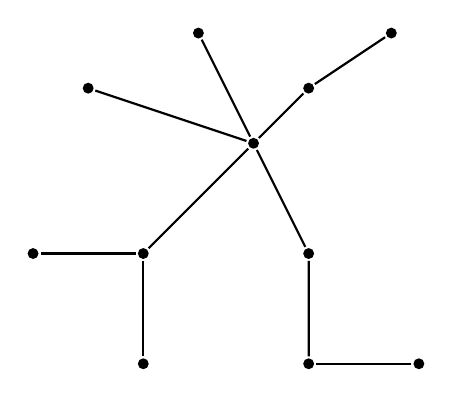
\begin{tikzpicture}[scale=0.7]
    %\draw[help lines] (-5,-5) grid (5,5);
        \def\x{-2}
        \GraphInit[vstyle=Normal]
        \SetVertexNormal[Shape=circle, FillColor=black, MinSize=2pt]
        \tikzset{VertexStyle/.append style = {inner sep = \inners, outer sep = \outers}}
        \Vertex[x=0,y=1,Lpos=270,NoLabel=true]{a}
        \Vertex[x=-1,y=3,Lpos=90,NoLabel=true]{b}
        \Vertex[x=1,y=2,Lpos=90,NoLabel=true]{c}
        \Vertex[x=-3,y=2,Lpos=90,NoLabel=true]{d}
        \Vertex[x=-2,y=-1,Lpos=90,NoLabel=true]{e}
        \Vertex[x=1,y=-1,Lpos=90,NoLabel=true]{f}
        \Vertex[x=-4,y=-1,Lpos=90,NoLabel=true]{g}
        \Vertex[x=-2,y=-3,Lpos=90,NoLabel=true]{h}
        \Vertex[x=1,y=-3,Lpos=90,NoLabel=true]{i}
        \Vertex[x=3,y=-3,Lpos=90,NoLabel=true]{j}
        \Vertex[x=2.5,y=3,Lpos=90,NoLabel=true]{k}
        
        
        \Edge(a)(b)
        \Edge(a)(c)
        \Edge(k)(c)
        \Edge(a)(d)
        \Edge(a)(e)
        \Edge(a)(f)
        \Edge(e)(g)
        \Edge(e)(h)
        \Edge(f)(i)
        \Edge(j)(i)
        
        
    \end{tikzpicture}
    \caption{A tree.}
    %  Some graph
    \label{fig:some_tree}
\end{figure}


\tdef{Chordal graphs} have many nice properties that enable the computation of different graph parameters in polynomial time~\citep{golumbic}. A \tdef{perfect elimination ordering} of a graph $G$ is an ordering $v_1, \dots, v_n$ of its vertices such that for the graph $G[\{v_i, \dots, v_n\}]$, $v_i$ is a simplicial vertex. As the name implies, chordal graphs are exactly the graphs where every cycle of size at least 4 has at least one chord. 

\begin{class_definition*}[Chordal Graph]
    For a graph $G$, the following properties are equivalent:
    \begin{itemize}
        \item[(i)] $G$ is chordal;
        \item[(ii)] It is $C_k$-free, for any $k \geq 4$;
        \item[(iii)] Every minimal cutset is a clique;
        \item[(iv)] It is the intersection graph of subtrees of a tree;
        \item[(v)] There is a perfect elimination ordering of its vertices.
    \end{itemize}
\end{class_definition*}

\begin{figure}[!htb]
    \centering
    % Define style for nodes
    
        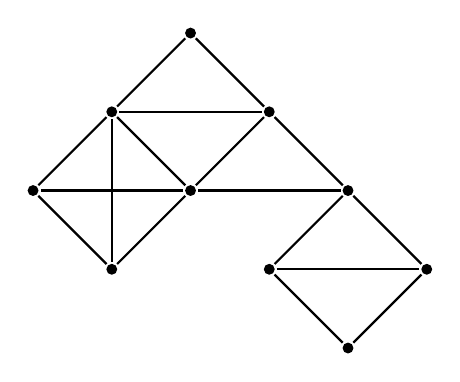
\begin{tikzpicture}
            \begin{scope}[rotate=90,scale=1]
                %\draw[help lines] (-4,-4) grid (4,4);
                \GraphInit[vstyle=Simple]
                \SetVertexSimple[Shape=circle, FillColor=black, MinSize=2pt]
                \tikzset{VertexStyle/.append style = {inner sep = \inners, outer sep = \outers}}
                \Vertex[x=0,y=2]{a}
                \Vertex[x=-1,y=3]{b}
                \Vertex[x=1,y=3]{c}
                \Vertex[x=0,y=4]{d}
                
                \Vertex[x=-1,y=1]{e}
                \Vertex[x=1,y=1]{f}
                
                \Vertex[x=-2,y=0]{h}
                \Vertex[x=0,y=0]{i}
                \Vertex[x=-1,y=-1]{j}
                
                \Vertex[x=2,y=2]{k}
                
                
                \Edge(a)(b)
                \Edge(a)(c)
                \Edge(a)(d)
                \Edge(b)(c)
                \Edge(b)(d)
                \Edge(d)(c)
                
                \Edge(c)(f)
                \Edge(c)(k)
                \Edge(k)(f)
                
                \Edge(a)(i)
                \Edge(a)(f)
                \Edge(i)(f)
                
                \Edge(e)(h)
                \Edge(e)(i)
                \Edge(e)(j)
                \Edge(h)(j)
                \Edge(i)(j)
            \end{scope}
        \end{tikzpicture}
    \hfill
        \begin{tikzpicture}
            \begin{scope}[rotate=90,scale=1]
                %\draw[help lines] (-4,-4) grid (4,4);
                \GraphInit[vstyle=Simple]
                \SetVertexSimple[Shape=circle, FillColor=black, MinSize=2pt]
                \tikzset{VertexStyle/.append style = {inner sep = \inners, outer sep = \outers}}
                
                \Vertex[x=-1.5,y=0]{c1}
                \Vertex[x=-0.5,y=0]{c2}
                \Vertex[x=0,y=1]{c3}
                \Vertex[x=0.5,y=2]{c4}
                \Vertex[x=0,y=3]{c5}
                \Vertex[x=1.5,y=2]{c6}
                
                \Edge(c1)(c2)
                \Edge(c2)(c3)
                \Edge(c3)(c4)
                \Edge(c4)(c5)
                \Edge(c4)(c6)
            \end{scope}
        \end{tikzpicture}
    \hfill
    \caption{A chordal graph and its clique tree.}
    %  Some graph
    \label{fig:some_chordal}
\end{figure}

For a chordal graph $G$, its \tdef{clique tree} is a tree $\mathcal{T}(G)$ such that: its vertex set, each of which is called a \tdef{bag}, is the set of maximal cliques of $G$, and, for every vertex $v$ of $G$, the set of bags which contains $v$ induces a subtree of $\mathcal{T}(G)$. It can be shown that such a tree satisfies property \textit{(iv)}.
For more on clique trees and other chordal graph properties please refer to~\citep{clique_tree}.

Not surprisingly, many subclasses of chordal graphs have also been studied, since even forests are chordal graphs.
A \tdef{block graph} is a chordal graph where every minimal cutset is a single vertex.
An \tdef{interval graph} is the intersection graph of a set of intervals over the real numbers.
A \tdef{split graph} is a graph whose vertex set can be partitioned into a clique and an independent set.

\tdef{Cographs} are the graphs $G$ such that either $G$ or its complement is disconnected. At first glance, such property may not seem very helpful to the algorithm designer, but it is equivalent to a very nice recursive definition, first given in~\citep{cographs}.
Given two graphs $G$ and $H$, we define their \tdef{disjoint union} as the graph $G \cup H$ with $V(G \cup H)= V(G) \cup V(H)$ and $E(G \cup H) = E(G) \cup E(H)$, and their \tdef{join} as the graph $G \otimes H$ with vertex set is $V(G \otimes H)= V(G) \cup V(H)$ and edge set $E(G \otimes H)= E(G) \cup E(H) \cup \{uv \mid u \in V(G), v \in V(H)\}$.

\begin{class_definition*}[Cograph]
    For a graph $G$, the following properties are equivalent:
    \begin{itemize}
        \item[(i)] $G$ is a cograph;
        \item[(ii)] $G$ is $P_4$-free;
        \item[(iii)] $G$ can be constructed from isolated vertices by successively applying disjoint union and join operations.
    \end{itemize}
\end{class_definition*}

\begin{figure}[!htb]
    \centering
    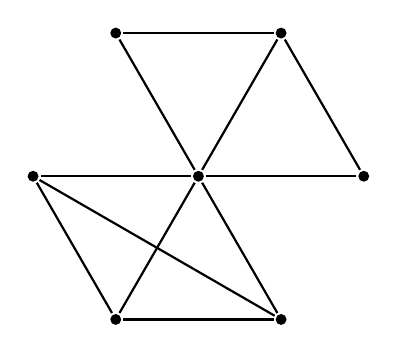
\begin{tikzpicture}[scale=0.7]
            \GraphInit[vstyle=Simple]
            \SetVertexSimple[Shape=circle, FillColor=black, MinSize=2pt]
            \tikzset{VertexStyle/.append style = {inner sep = \inners, outer sep = \outers}}
            \Vertices[unit=3]{circle}{a,b,c,d,e,f}
            \Vertex[x=0,y=0]{g}
            
            \Edge(b)(a)
            \Edge(c)(b)
            
            \Edge(e)(f)
            \Edge(e)(d)
            \Edge(f)(d)
            
            \Edge(g)(a)
            \Edge(g)(b)
            \Edge(g)(c)
            \Edge(g)(d)
            \Edge(g)(e)
            \Edge(g)(f)
        \end{tikzpicture}
    \caption{A cograph.}
    \label{fig:some_cograph}
\end{figure}

Another important class on graph theory, and one with a very long history of research, is the class of \textit{regular graphs}.
A graph $G$ is regular if all of vertices of $G$ have the same degree, and is $k$-regular if $\deg(v) = k$ for all $v \in V(G)$.
Despite its simplicity, regular graphs appear in many different scenarios, such as in the E$\Delta$CC conjecture on \pname{Equitable Coloring}, a conjecture for \pname{Internal Partitions}, but even more in terms of algebraic graph theory~\citep{godsil}, a field dedicated to the analysis of many graph parameters through algebraic methods, such as spectral decompositions, graph polynomials, and interlacing.
In particular, by using the eigenvalues of the adjacency matrix of a graph, or its Laplacian matrix, it is possible to derive bounds for a large collection of parameters, such as independence number and chromatic number, usually in polynomial time.
Regular graphs, in particular, benefit greatly from this approach, with stronger results for this class when compared to other classes.




%\chapter{Preliminaries and Related Work}
\label{ch:prelims}

\section{Basic Definitions}
\label{sec:basic_defs}

We denote by $[n] = \{1, \dots, n\}$.
A (\tdef{multi})\tdef{family} is a (multi)set of sets.
The \tdef{power set} $2^S$ of a set $S$ is the family of all subsets of $S$.
A \tdef{k-partition} of $S$ into $k$ sets is denoted by $S \sim \{S_1, \dots, S_k\}$ such that $S_i \cap S_j = \emptyset$ and $\bigcup_{i \leq k} S_i = S$.
A \tdef{k-(multi)cover} of $S$ is a (multi)family $\{S_1, \dots, S_k\}$ of subsets of $S$ such that $\bigcup_{i \in [k]} S_i = S$.
A (multi)family $\mathcal{F}$ satisfies the \tdef{Helly condition} or \tdef{Helly property} if and only if, for every pairwise intersecting subfamily $\mathcal{F}'$ of $\mathcal{F}$, $\bigcap_{F \in \mathcal{F}'} F \neq \emptyset$.

A \tdef{simple graph} of \tdef{order} (or \tdef{size}) $n$ is an ordered pair $G = (V(G), E(G))$, where $V(G)$ is its \tdef{vertex set} of cardinality $n$ and its \tdef{edge set}, $E(G)$, is a family of subsets of $V(G)$, each of cardinality two. A graph is \tdef{trivial} if $|V(G)| = 1$.
Instead of $\{u,v\} \in E(G)$, we identify an edge by $uv$, simply due to convenience. Moreover, when there is no ambiguity, we denote $V(G)$ by $V$, $E(G)$ by $E$, $|V|$ as $n$ and $|E|$ as $m$.

We say that two vertices $u,v \in V$ are \tdef{adjacent} or \tdef{neighbours} if $uv \in E$.
A graph $G' = (V', E')$ is a \tdef{subgraph} of $G$ if $V' \subseteq V$ and $E' \subseteq E$.
If $E' = \{uv \in E \mid u,v \in V'\}$ we say that $V'$ \tdef{induces} $G'$, $G' = G[V']$ and that $G'$ is the \tdef{induced subgraph} of $G$ by $V$.
For simplicity, we denote by $G - v$ the graph $G[V(G) \setminus \{v\}]$ and, similarly, for $S \subseteq V(G)$, $G \setminus S$ is equivalent to $G[V(G) \setminus S]$.

The \tdef{open neighbourhood}, or just \tdef{neighbourhood} of a vertex $v$ in $G$ is given by $N_G(v) = \{u \mid uv \in E(G)\}$, its \tdef{closed neighbourhood} by $N_G[v] = N_G(v) \cup \{v\}$ and its \tdef{degree} by $d_G(v) = |N_G(v)|$.
A vertex is \tdef{simplicial} if its neighbours are pairwise adjacent.
For a set $S \subseteq V$, we denote its open and closed neighbourhood as $N_G(S) = \bigcup_{v \in S} N_G(v) \setminus S$, $N_G[S] = N_G(S) \cup S$ and $d_G(S) = |N_G(S)|$, respectively.
The \tdef{complement} $\overline{G}$ of $G$ is defined as $V(\overline{G}) = V(G)$ and $E(\overline{G}) = \{uv | uv \notin E\}$.
Given a graph $G$, we denote its \tdef{maximum degree} by $\Delta(G)$ and \tdef{minimum degree} by $\delta(G)$.
A graph $G$ is \tdef{$k$-regular} if , for every $u \in V(G)$, $d_G(u) = k$.

Two vertices $u,v$ are \tdef{false twins} if $N_G(u) = N_G(v)$ and \tdef{true twins} if $N_G[u] = N_G[v]$. $u,v$ are of the same \tdef{type} if they are either true or false twins.
Being of the same type is an equivalence relation~\citep{neighbourhood_diversity}, and the number of different types on a graph $G$ is called its \tdef{neighbourhood diversity}, $\nd(G)$.

Two graphs $G$ and $H$ are \tdef{isomorphic} if and only if there is a bijection $f: V(G) \mapsto V(H)$ such that $uv \in E(G) \Leftrightarrow f(u)f(v) \in E(H)$.
We denote isomorphism by $G \simeq H$.
A graph $G$ is said to be \tdef{free} of a graph $H$, or $H$-free, if there is no induced subgraph $G'$ of $G$ such that $G'$ and $H$ are isomorphic.

The \tdef{path} of length $k$, or $P_k$, is a graph with $k$ vertices $v_1 \dots v_k$ such that $v_iv_j \in E(P_k)$ if and only if $j = i+1$. Moreover, we say that $v_1, v_k$ are the \tdef{extremities}, or \tdef{endvertices}, of $P_k$ and all other $v_i$ are its \tdef{inner} vertices.
The length of a path is the number of edges contained in it, that is, $P_k$ has length $k-1$.
An \tdef{induced path} of $G$ is a subgraph $G'$ of $G$ that is isomorphic to a path.
A \tdef{cycle} with  $k \geq 3$ vertices is a path with $k$ vertices plus the edge $v_kv_1$; analogously, the length of a cycle is defined as the number of edges it contains.
An \tdef{induced cycle} of $G$ is an induced subgraph $G'$ of $G$ that is isomorphic to a cycle.
A \tdef{chord} in a cycle $C$ of length at least 4 is an edge between two non-consecutive vertices of $C$.
The \tdef{girth} of $G$, denoted by $\girth(G)$, is the length of the smallest induced cycle of $G$.
A \tdef{hole} is a chordless cycle of length at least 4; it is an even-hole if it has an even number of vertices, or an odd-hole, otherwise. An \tdef{anti-hole} is the complement of a hole.
$G$ is \tdef{acyclic} if and only if there is no induced cycle in $G$.


A graph $G$ is \tdef{connected} if and only if there is an induced path between every pair $u,v \in V$.
A \tdef{connected component}, or simply a \tdef{component}, of $G$ is a maximal connected induced subgraph of $G$.
Given a graph $G$, the \tdef{distance} $\dist_G(u,v)$ between two vertices $u,v$ in $G$ is the minimum number of edges in any path between them.
If $u,v$ are in different components, we say that $\dist_G(u,v) = \infty$.
The \tdef{diameter} of a connected graph $G$ is defined as the length of the longest shortest path between any pair of vertices $u,v \in V(G)$.
The \tdef{$k$-th power} $G^k$ of a graph $G$ is the graph where $V(G^k) = V(G)$ and $E(G^k) = \{uv \mid \dist_G(u,v) \leq k\}$.
When the graph in question is clear, we will omit the $G$ subscript.

An \tdef{articulation point}, \tdef{cut point} or \tdef{cut vertex} of a connected graph $G$ is a vertex $v$ such that $G - v$ is disconnected.
A \tdef{bridge} is an edge of $G$ whose removal increases the number of connected components of $G$.
$G$ is \tdef{biconnected} if $G$ is connected and does not have a cut vertex.
A \tdef{cutset} of a connected graph $G$ is a set $S \subset V$ such that $G \setminus S$ is disconnected.
In particular, a cut vertex is a cutset of size one.

The \tdef{complete} graph $K_n$ of order $n$ is a graph where every pair of vertices is adjacent.
A \tdef{clique} of $G$ with $n$ vertices is an induced subgraph of $G$ isomorphic to $K_n$.
An \tdef{independent set} of $G$ with $n$ vertices is an induced subgraph of $G$ isomorphic to $\overline{K_n}$.
We denote by $\omega(G)$ and $\alpha(G)$ the size of the maximum induced clique and maximum independent set of a given $G$.
Both of these values are examples of \tdef{graph parameters}, that is, a value that describes some property of interest of the underlying graph.
Determining certain parameters of a generic graph $G$ is efficient (such as $\Delta(G)$ and $\delta(G)$); however, others (such as $\omega(G)$ and $\alpha(G)$) are widely believed to be hard to ascertain.

A graph $G$ is \tdef{bipartite} if $V(G) \sim \{X, Y\}$ such that both $X$ and $Y$ are independent sets. Such property implies that a graph is bipartite if and only if it is $C_{2k+1}$-free, for any $k \geq 1$.
A \tdef{biclique} $K_{n_1,n_2}$ is a bipartite graph with $|X| = n_1$, $|Y| = n_2$ and $uv \in E(G)$ for every pair $u \in X$ and $v \in Y$.
A \tdef{star} is a biclique with $|X| = 1$ and $|Y| \geq 1$.
Clearly, we can also define \tdef{induced bicliques} and \tdef{induced stars} much like induced cliques.

A \tdef{hypergraph} $\hypergraph = (V, \mathcal{E})$ is a natural generalization of a graph.
That is, $V(\hypergraph)$ is its vertex set and $\mathcal{E} \subseteq 2^{V}$ its \tdef{hyperedge} set~\citep{hypergraphs}.
A graph $G$ is said to be a \tdef{host} of $\mathcal{H}$ if $V(G) = V(\hypergraph)$, every hyperedge of $\hypergraph$ induces a connected subgraph of $G$ and every edge of $G$ is contained in at least one hyperedge of $\mathcal{H}$.

A \tdef{transversal} of a hypergraph $\hypergraph$ is a set $X \subseteq V(\hypergraph)$ such that, for every hyperedge $\varepsilon \in \mathcal{E}(\hypergraph)$, $X \cap \varepsilon \neq \emptyset$.
If $X$ is not a transversal we say that it is an \tdef{oblique}.

The \tdef{clique hypergraph} $\Hyper{C}(G)$ of a graph $G$ is the hypergraph on the same vertex set of $G$ and with hyperedge set equal to the family of maximal cliques of $G$.
Similarly, the \tdef{biclique hypergraph} $\Hyper{B}(G)$ of a graph $G$ is the hypergraph on the same vertex set of $G$ and with hyperedge set equal to the family of maximal bicliques of $G$.

%Maybe talk about hypergraphs here, not sure where

\section{Complexity Classes}

We discuss problems in different complexity classes; in particular, we work with the usual $\P$ and $\NP$ classes, but also the $\SiP{2}$ class of the \tdef{polynomial hierarchy}~\citep{polynomial_hierarchy}.
We say that an algorithm is \tdef{efficient} if its running time is bounded by a polynomial on the size of the input and that a problem belonging to $\NPH$ is most likely intractable.
As such, our complexity results will be given either by efficient algorithms or polynomial reductions from $\NPH$ problems.

Besides the classic complexity classes, we also deal with the much newer field of \tdef{parameterized complexity} (also called \tdef{multivariate complexity}).
In this area, algorithms are designed and analyzed not only with respect to the size of the input object, but also with other \tdef{parameters} of the input.
A parameter can be anything, from the size of the problem's solution to a measurement of how complicated the structure of the instance is.

A problem is said to be \tdef{fixed-parameter tractable} (or FPT) when \tdef{parameterized by} $k$ if there is an algorithm with running time $f(k)n^{\bigO{1}}$, where $n$ is the size of the input object.
We denote complexities of this form by $\bigOs{f(k)}$.
In fact, we shall use $\bigOs{}$ to omit polynomial factors of the running time; that is, an algorithm with complexity $2^{f(n)}\text{poly}(n)$ is said to execute in $\bigOs{2^{f(n)}}$.
In a slight abuse of notation, $k$ is simultaneously the parameter we are working with and the value of such parameter.
An instance of a parameterized algorithm is, therefore, the pair $(x,k)$, with $x$ the input object and $k$ as previously defined.
The class of all problems that admit an FPT algorithm is the class $\FPT$.
If an algorithm presents running time $\bigO{n^{f(k)}}$, for some computable function on $k$,  we say it is an XP (slicewise polynomial) algorithm, and the corresponding problem it solves is in $\XP$. 

Much like classical univariate theory, some problems do not appear to admit an FPT algorithm for certain parameterizations. In particular, its widely believed that finding a clique of size $k$ in a graph, parameterized by $k$, is not in $\FPT$.
In an analogue to the classical case, hardness results are usually given by what are called \tdef{parameterized reductions}.

\begin{class_definition*}[Parameterized Reduction]
    A parameterized reduction from problem $\Pi$ to problem $\Pi'$ is a transformation from an instance $(x, k)$ of $\Pi$ to an instance $(x',k')$ of $\Pi'$ such that:
    \begin{enumerate}
        \item There is a solution to $(x,k)$ if and only if there is a solution to $(x',k')$;
        \item $k' \leq g(k)$ for some computable function $g$;
        \item The transformation's running time is $\bigOs{f(k)}$.
    \end{enumerate}
\end{class_definition*}

Note that the constraints imposed by parameterized reductions are quite similar to those imposed by polynomial reductions.
We ask that $k'$ does not depend on $|x|$ - which doesn't always happen with polynomial reductions - but, at the same time, allow $\FPT$ time for the transformation, instead of the more restrictive polynomial time.
These differences imply that polynomial reductions and parameterized reductions are incomparable, with some rare cases where the transformation is both polynomial and parameterized.

Unlike the theory of $\NPcness$, where most hard problems are equivalent to each other under polynomial reductions, in parameterized complexity problems seem to be distributed along a hierarchy of difficulty.
Before handling the classes themselves, we must first define the problems of parameterized complexity that play the same role as \tsc{satisfability} for the classical theory. 

The \tdef{depth} of a circuit is the length (in terms of number of gates) of the longest path from any one variable to the output.
The \tdef{weft} of a circuit is the the maximum number of gates with more than 2 input variables in any path from any one variable to the circuit's output.
The circuits with weft $t$ and depth $d$, denoted by \pname{wcs}$_{t,d}$, will be the fundamental problems of the $t$-th level of our hierarchy.

\pproblem{weighted circuit satisfability of weft $t$ and depth $d$ (\pname{wcs}$_{t,d}$)}{A Boolean circuit $C$ with $n$ variables, weft $t$ and depth $d$.}{A positive integer $k$.}{Is $C$ satisfiable with exactly $k$ variables set to $\TRUEt$?}

\begin{class_definition*}[$\W$-hierarchy]
    For $t \geq 1$, a parameterized problem $\Pi$ is in $\W[t]$ if there is a parameterized reduction from $\tsc{wsc}_{t,d}$ to it, for some $d \geq 1$. Moreover,
    \begin{equation*}
        \FPT \subseteq \W[1] \subseteq \W[2] \subseteq \cdots \subset \XP
    \end{equation*}
\end{class_definition*}

For further reading and other more insightful discussions on the subject, we point to~\citep{downey_fellows} and~\citep{cygan_parameterized}, from where most of the given definitions come from. 

\section{Intersection Graphs}
\label{sec:intersections}

The \tdef{intersection graph} of a multifamily $\mathcal{F} \subseteq 2^S$, denoted by $G = \Omega(\mathcal{F})$ is the graph of order $|\mathcal{F}|$ and, for every $F_u, F_v \in \mathcal{F}$, $uv \in E(G) \Leftrightarrow F_u \cap F_v \neq \emptyset$.
Any $\mathcal{F}$ such that $\Omega(\mathcal{F}) \simeq G$ is a \tdef{set representation} of $G$.
A known theorem states that every graph is the intersection graph of a family of subgraphs of a graph~\citep{intersection_graphs}.

An \tdef{edge clique cover} $\mathcal{Q} = \{Q_1, \dots, Q_n\}$ of a graph $G$ is a (multi)family of cliques of $G$ such that every edge of $G$ is contained in at least one element of $\mathcal{Q}$.
The \tdef{dual edge clique cover} of a set representation $\mathcal{F} = \{F_1, \dots, F_n\}$, with $|\bigcup_{i \leq n} F_i| = m$, is defined as $\mathcal{Q}(\mathcal{F}) = \{Q_1, \dots, Q_m\}$ such that $Q_j = \{i \mid j \in F_i\}$.
The \tdef{dual set representation} of an edge clique cover $\mathcal{Q} = \{Q_1, \dots, Q_m\}$, with $|\bigcup_{j \leq m} Q_j| = n$, is $\mathcal{F}(\mathcal{Q}) = \{F_1, \dots, F_n\}$ with $F_i = \{j \mid i \in Q_j\}$.

Some interesting intersection graphs are usually defined in terms of the intersection of structures of other graphs. For instance, \tdef{line graphs} are precisely the graphs that are the intersection graphs of the edges of a graph; \tdef{clique graphs} are the intersection graphs of the maximal induced cliques of a graph.
Both of these classes, however have nice characterizations in terms of edge clique covers, which are commonly called \tdef{Krausz-type characterizations}.

\begin{class_definition*}[Line Graph]
    $G$ is a line graph if and only if there is an edge clique cover $\mathcal{Q}$ of $G$ such that both conditions hold:
        \begin{itemize}
            \item[(i)] Every vertex of $G$ appears in exactly two members of $\mathcal{Q}$;
            \item[(ii)] Every edge of $G$ is in only one member of $\mathcal{Q}$.
        \end{itemize}
\end{class_definition*}

\begin{class_definition*}[Clique Graph]
    $G$ is a clique graph if and only if it there is an edge clique cover of $G$ satisfying the Helly property.
\end{class_definition*}

\begin{figure}[!htb]
    \centering
        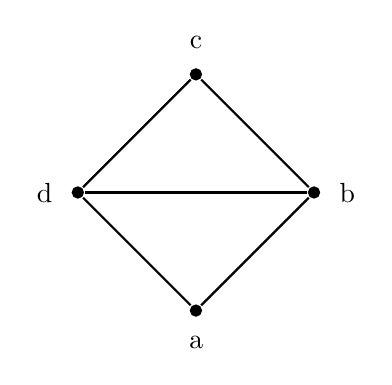
\begin{tikzpicture}
            \begin{scope}[rotate=-90,scale=0.5]
                \def\x{-2}
                \GraphInit[vstyle=Normal]
                \SetVertexNormal[Shape=circle, FillColor=black, LineWidth=1pt,MinSize=2pt,]
                \tikzset{VertexStyle/.append style = {inner sep = \inners, outer sep = \outers}}
                \Vertices[Lpos=270,Ldist=3pt,LabelOut=TRUE,unit=3]{circle}{a,b,c,d}
                \Edge(a)(b)
                \Edge(a)(d)
                \Edge(c)(b)
                \Edge(d)(b)
                \Edge(c)(d)
            \end{scope}
        \end{tikzpicture}
    \hfill
        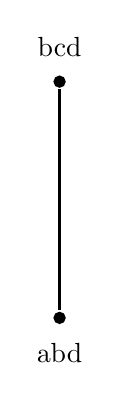
\begin{tikzpicture}
            \begin{scope}[rotate=-90,scale=0.5]
                \def\x{-2}
                \GraphInit[vstyle=Normal]
                \SetVertexNormal[Shape=circle, FillColor=black, LineWidth=1pt,MinSize=2pt,]
            \tikzset{VertexStyle/.append style = {inner sep = \inners, outer sep = \outers}}
                \Vertices[Lpos=270,Ldist=3pt,LabelOut=TRUE,unit=3]{circle}{abd,bcd}
                \Edge(abd)(bcd)
            \end{scope}
        \end{tikzpicture}
    \hfill
        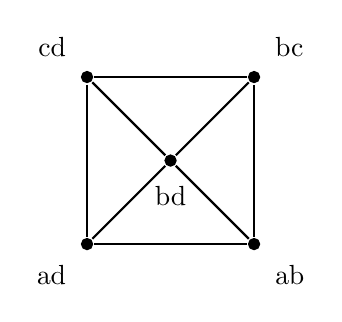
\begin{tikzpicture}
            \begin{scope}[rotate=315,scale=0.5]
                \def\x{-2}
                \GraphInit[vstyle=Normal]
                \SetVertexNormal[Shape=circle, FillColor=black, LineWidth=1pt,MinSize=2pt,]
            \tikzset{VertexStyle/.append style = {inner sep = \inners, outer sep = \outers}}
                \Vertices[Lpos=315,Ldist=3pt,LabelOut=TRUE,unit=3]{circle}{ab,bc,cd,ad}
                \Vertex[Lpos=270,Ldist=3pt,LabelOut=TRUE,unit=3,x=0,y=0]{bd}
                \Edge(ab)(bc)
                \Edge(ab)(ad)
                \Edge(bc)(cd)
                \Edge(cd)(ad)
                \Edge(bd)(ab)
                \Edge(bd)(ad)
                \Edge(bd)(cd)
                \Edge(bd)(bc)
            \end{scope}
        \end{tikzpicture}
    \hfill
    \caption{A graph (left), its clique graph (center) and its line graph (right).}
    %  Some graph
    \label{fig:my_label}
\end{figure}

The recognition of line graphs is known to be efficient, as shown by~\citep{line_dynamic,line_nich,line_naor}.
For clique graphs, however, the situation was not so simple, and the complexity of clique graph recognition was left open for several years, finally being proven to be $\NPc$ by~\citep{clique_recognition} with a quite complicated argument.

Recently, \citep{biclique_graph} defined the \tdef{biclique graph} as the intersection graph of the maximal induced bicliques of a graph.
Their characterization for even limited input graphs, however, is a bit convoluted, and even checking membership in $\NP$ does not appear to be an easy task.

For other classical results in the area we point to~\citep{intersection_graphs}, from where most of the given definitions come from.

\section{Graph Classes}
\label{sec:graph_classes}

Most problems in graph theory can be tackled with an arbitrary input, that is, there is no particular property that we can exploit; this can happen if the considered application is too broad or little is known about its domain.
However, it might be possible to guarantee certain characteristics for the given graph, either due constraints of the application~\citep{fernando_chordal} or due to theoretical interest.
Regardless, such guarantees might be strong enough to provide an efficient algorithm to an otherwise $\NPH$ problem.
When constraining our analysis to certain graphs, we refer to the family of all graphs that satisfy the same properties as a \tdef{graph class}.
A subfamily of a class that satisfies additional properties is referred to as a \tdef{subclass}.
For (much) more on graph classes, \citep{classes_survey} give an extensive survey of much of the work done on the field until the late 1990s.

In this section, we review some of the most studied classes and some of their properties that will aid us in the design of our algorithms.

A graph is a \tdef{tree} $T$ if it is a connected acyclic graph or, equivalently, the connected graph such that, between every pair of vertices $u$ and $v$, there exists a unique path.
The vertices of degree one of a tree are called its \tdef{leaves}, and all others are \tdef{inner} nodes. A \tdef{subtree} $T'$ of a tree $T$ is a connected subgraph which, clearly, must also be a tree.
A \tdef{rooted tree} $T_v$ is a tree with a special vertex $v$, called its \tdef{root}.
Rooted trees offer a straight forward ordering of the vertices of a tree and a nice way to decompose problems into smaller instances and combine their solutions.
A \tdef{rooted subtree} $T_u$ of $T_v$ is the subgraph of $T_v$ induced by $u$ and all vertices of $T_v$ whose path to $v$ passes through $u$.
The vertices in $T_u \setminus \{u\}$ are called the \tdef{descendants} of $u$ and its neighbours are its \tdef{children}.

A \tdef{forest} is a graph where every connected component is a tree.
Many problems which are usually quite hard for general graphs, or even some classes, usually have a straightforward answer for forests, either using a greedy strategy or a slightly more sofisticated dynamic programming idea.

\begin{figure}
    \centering
    % Define style for nodes
    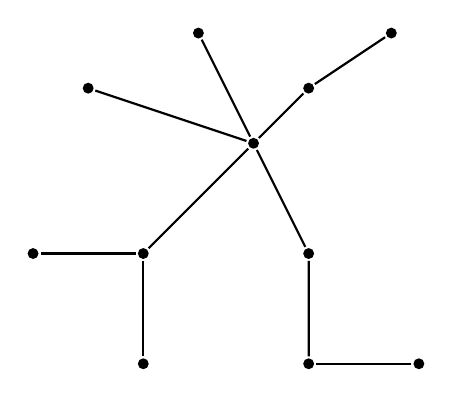
\begin{tikzpicture}[scale=0.7]
    %\draw[help lines] (-5,-5) grid (5,5);
        \def\x{-2}
        \GraphInit[vstyle=Normal]
        \SetVertexNormal[Shape=circle, FillColor=black, MinSize=2pt]
        \tikzset{VertexStyle/.append style = {inner sep = \inners, outer sep = \outers}}
        \Vertex[x=0,y=1,Lpos=270,NoLabel=true]{a}
        \Vertex[x=-1,y=3,Lpos=90,NoLabel=true]{b}
        \Vertex[x=1,y=2,Lpos=90,NoLabel=true]{c}
        \Vertex[x=-3,y=2,Lpos=90,NoLabel=true]{d}
        \Vertex[x=-2,y=-1,Lpos=90,NoLabel=true]{e}
        \Vertex[x=1,y=-1,Lpos=90,NoLabel=true]{f}
        \Vertex[x=-4,y=-1,Lpos=90,NoLabel=true]{g}
        \Vertex[x=-2,y=-3,Lpos=90,NoLabel=true]{h}
        \Vertex[x=1,y=-3,Lpos=90,NoLabel=true]{i}
        \Vertex[x=3,y=-3,Lpos=90,NoLabel=true]{j}
        \Vertex[x=2.5,y=3,Lpos=90,NoLabel=true]{k}
        
        
        \Edge(a)(b)
        \Edge(a)(c)
        \Edge(k)(c)
        \Edge(a)(d)
        \Edge(a)(e)
        \Edge(a)(f)
        \Edge(e)(g)
        \Edge(e)(h)
        \Edge(f)(i)
        \Edge(j)(i)
        
        
    \end{tikzpicture}
    \caption{A tree.}
    %  Some graph
    \label{fig:some_tree}
\end{figure}


\tdef{Chordal graphs} have many nice properties that enable the computation of different graph parameters in polynomial time~\citep{golumbic}. A \tdef{perfect elimination ordering} of a graph $G$ is an ordering $v_1, \dots, v_n$ of its vertices such that for the graph $G[\{v_i, \dots, v_n\}]$, $v_i$ is a simplicial vertex. As the name implies, chordal graphs are exactly the graphs where every cycle of size at least 4 has at least one chord. 

\begin{class_definition*}[Chordal Graph]
    For a graph $G$, the following properties are equivalent:
    \begin{itemize}
        \item[(i)] $G$ is chordal;
        \item[(ii)] It is $C_k$-free, for any $k \geq 4$;
        \item[(iii)] Every minimal cutset is a clique;
        \item[(iv)] It is the intersection graph of subtrees of a tree;
        \item[(v)] There is a perfect elimination ordering of its vertices.
    \end{itemize}
\end{class_definition*}

\begin{figure}[!htb]
    \centering
    % Define style for nodes
    
        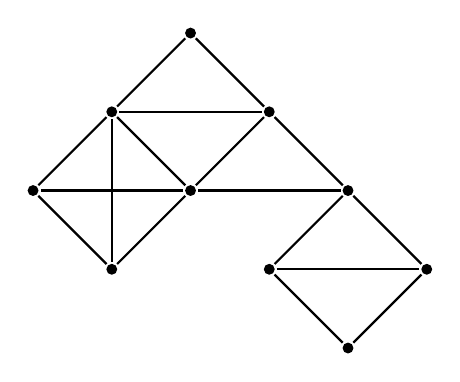
\begin{tikzpicture}
            \begin{scope}[rotate=90,scale=1]
                %\draw[help lines] (-4,-4) grid (4,4);
                \GraphInit[vstyle=Simple]
                \SetVertexSimple[Shape=circle, FillColor=black, MinSize=2pt]
                \tikzset{VertexStyle/.append style = {inner sep = \inners, outer sep = \outers}}
                \Vertex[x=0,y=2]{a}
                \Vertex[x=-1,y=3]{b}
                \Vertex[x=1,y=3]{c}
                \Vertex[x=0,y=4]{d}
                
                \Vertex[x=-1,y=1]{e}
                \Vertex[x=1,y=1]{f}
                
                \Vertex[x=-2,y=0]{h}
                \Vertex[x=0,y=0]{i}
                \Vertex[x=-1,y=-1]{j}
                
                \Vertex[x=2,y=2]{k}
                
                
                \Edge(a)(b)
                \Edge(a)(c)
                \Edge(a)(d)
                \Edge(b)(c)
                \Edge(b)(d)
                \Edge(d)(c)
                
                \Edge(c)(f)
                \Edge(c)(k)
                \Edge(k)(f)
                
                \Edge(a)(i)
                \Edge(a)(f)
                \Edge(i)(f)
                
                \Edge(e)(h)
                \Edge(e)(i)
                \Edge(e)(j)
                \Edge(h)(j)
                \Edge(i)(j)
            \end{scope}
        \end{tikzpicture}
    \hfill
        \begin{tikzpicture}
            \begin{scope}[rotate=90,scale=1]
                %\draw[help lines] (-4,-4) grid (4,4);
                \GraphInit[vstyle=Simple]
                \SetVertexSimple[Shape=circle, FillColor=black, MinSize=2pt]
                \tikzset{VertexStyle/.append style = {inner sep = \inners, outer sep = \outers}}
                
                \Vertex[x=-1.5,y=0]{c1}
                \Vertex[x=-0.5,y=0]{c2}
                \Vertex[x=0,y=1]{c3}
                \Vertex[x=0.5,y=2]{c4}
                \Vertex[x=0,y=3]{c5}
                \Vertex[x=1.5,y=2]{c6}
                
                \Edge(c1)(c2)
                \Edge(c2)(c3)
                \Edge(c3)(c4)
                \Edge(c4)(c5)
                \Edge(c4)(c6)
            \end{scope}
        \end{tikzpicture}
    \hfill
    \caption{A chordal graph and its clique tree.}
    %  Some graph
    \label{fig:some_chordal}
\end{figure}

For a chordal graph $G$, its \tdef{clique tree} is a tree $\mathcal{T}(G)$ such that: its vertex set, each of which is called a \tdef{bag}, is the set of maximal cliques of $G$, and, for every vertex $v$ of $G$, the set of bags which contains $v$ induces a subtree of $\mathcal{T}(G)$. It can be shown that such a tree satisfies property \textit{(iv)}.
For more on clique trees and other chordal graph properties please refer to~\citep{clique_tree}.

Not surprisingly, many subclasses of chordal graphs have also been studied, since even forests are chordal graphs. A \tdef{block graph} is a chordal graph where every minimal cutset is a single vertex. An \tdef{interval graph} is the intersection graph of a set of intervals over the real numbers. A \tdef{split graph} is a graph whose vertex set can be partitioned into a clique and an independent set.

\tdef{Cographs} are the graphs $G$ such that either $G$ or its complement is disconnected. At first glance, such property may not seem very helpful to the algorithm designer, but it is equivalent to a very nice recursive definition, first given in~\citep{cographs}.
Given two graphs $G$ and $H$, we define their \tdef{disjoint union} as the graph $G \cup H$ with $V(G \cup H)= V(G) \cup V(H)$ and $E(G \cup H) = E(G) \cup E(H)$, and their \tdef{join} as the graph $G \otimes H$ with vertex set is $V(G \otimes H)= V(G) \cup V(H)$ and edge set $E(G \otimes H)= E(G) \cup E(H) \cup \{uv \mid u \in V(G), v \in V(H)\}$.

\begin{class_definition*}[Cograph]
    For a graph $G$, the following properties are equivalent:
    \begin{itemize}
        \item[(i)] $G$ is a cograph;
        \item[(ii)] $G$ is $P_4$-free;
        \item[(iii)] $G$ can be constructed from isolated vertices by successively applying disjoint union and join operations.
    \end{itemize}
\end{class_definition*}

\begin{figure}[!htb]
    \centering
    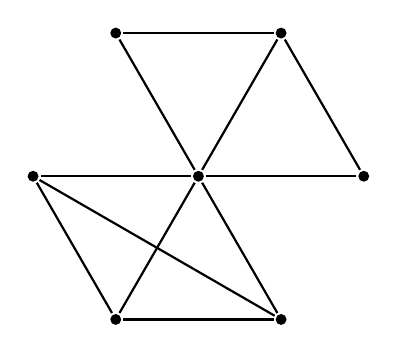
\begin{tikzpicture}[scale=0.7]
            \GraphInit[vstyle=Simple]
            \SetVertexSimple[Shape=circle, FillColor=black, MinSize=2pt]
            \tikzset{VertexStyle/.append style = {inner sep = \inners, outer sep = \outers}}
            \Vertices[unit=3]{circle}{a,b,c,d,e,f}
            \Vertex[x=0,y=0]{g}
            
            \Edge(b)(a)
            \Edge(c)(b)
            
            \Edge(e)(f)
            \Edge(e)(d)
            \Edge(f)(d)
            
            \Edge(g)(a)
            \Edge(g)(b)
            \Edge(g)(c)
            \Edge(g)(d)
            \Edge(g)(e)
            \Edge(g)(f)
        \end{tikzpicture}
    \caption{A cograph.}
    \label{fig:some_cograph}
\end{figure}

A graph $G$ is \tdef{distance-hereditary} if and only if for every $u,v$ and in every induced subgraph $H$ that preserves the connectivity between $u$ and $v$, $\dist_H(u,v) = \dist_G(u,v)$~\citep{distance_hereditary}.
A graph is \tdef{ptolemaic} if, for any $u,v,w,x$, $\dist(u,v) \dist(w,x) \leq \dist(u,w) \dist(v,x) + \dist(u,x) \dist(v,w)$~\citep{ptolemaic}.
Cographs and ptolemaic graphs are special cases of distance-hereditary graphs. In particular, ptolemaic graphs are exactly the graphs that are chordal and distance-hereditary.

\section{Coloring Problems}

A \tdef{k-coloring} of a graph $G$ is a $k$-partition $\varphi = \{\varphi_1, \dots,\varphi_k\}$ of $V(G)$.
Each $\varphi_i$ is a \tdef{color class} and $v \in V(G)$ is \tdef{colored} with color $i$ if and only if $v \in \varphi_i$.
In a slight abuse of notation, we use $\varphi(v)$ to denote the color of $v$ and, for $X \subseteq V(G)$, $\varphi(X) = \bigcup_{v \in X} \{\varphi(v)\}$.

\subsection{Proper Coloring}

A \tdef{proper k-coloring} of $G$ is a $k$-coloring such that each $\varphi_i$ is an independent set.
In the literature, proper coloring is usually referenced to as \tdef{vertex coloring}, a convention we also adopt.
If $G$ has a proper $k$-coloring we say that $G$ is \tdef{k-colorable}.
The smallest integer $k$ such that $G$ is $k$-colorable is called the \tdef{chromatic number} $\chi(G)$ of $G$.
The natural decision problem associated with vertex coloring simply asks whether or not a given graph is $k$-colorable.

\problem{vertex coloring}{A graph $G$ and a positive integer $k$.}{Is $G$ $k$-colorable?}


\begin{figure}[!htb]
    \centering
    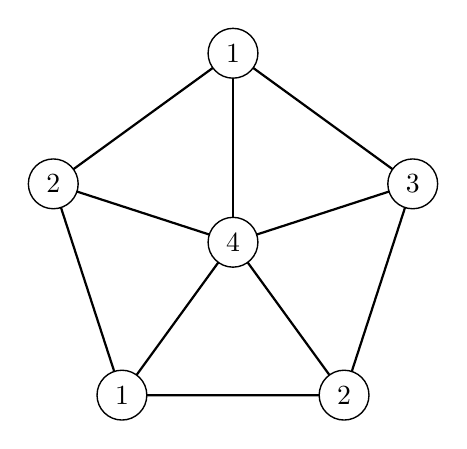
\begin{tikzpicture}[rotate=90,scale=0.6]
            %\draw[help lines] (-5,-5) grid (5,5);
            \GraphInit[vstyle=Simple]
            \SetVertexSimple[Shape=circle, FillColor=black, MinSize=2pt]
            \tikzset{VertexStyle/.append style = {inner sep = \inners, outer sep = \outers}}
            \SetUpVertex[Ldist=3pt]
            \grWheel[prefix=a]{6}
            \AssignVertexLabel{a}{1,2,1,2,3,4}
        \end{tikzpicture}
    \caption{An optimal proper coloring.}
    \label{fig:prop_color}
\end{figure}

Determining if a given instance of \textsc{vertex coloring} is a $\YES$ instance is a classic problem in both graph theory and algorithmic complexity, being a known $\NPc$ problem.
Some particular cases of \textsc{vertex coloring} are still $\NPc$.
For instance, even if we fix $k=3$ or restrict the input to $K_3$-free graphs the problem does not get any easier.

It is worth to point out the subtle difference between the parameter $k$ being part of the input or being \tdef{fixed}.
Informally, when $k$ is fixed, we are willing to pay exponential time only on $k$ to solve our problem, whereas when $k$ is part of the input, we are not.
Note that when we fix $k$ and find an $f(k)n^{\bigO{1}}$ time algorithm, we show that the problem is in $\FPT$ when parameterized by $k$.
The fact that $3$-coloring is $\NPc$ is evidence that \textsc{vertex coloring} parameterized by the number of colors is not in $\FPT$, otherwise we would have an $f(3)n^{\bigO{1}}$ algorithm, which would imply that $\P = \NP$. 
For the remainder of this work, when dealing with fixed $k$, we will include the fixed parameter in the name of the problem, such as in \textsc{vertex $k$-coloring} or \textsc{weighted circuit satisfability of weft $t$ and depth $d$}.

For an unconstrained input, \textsc{vertex coloring} is hard to approximate to a factor of $n^{1-\epsilon}$, for any $\epsilon > 0$, unless some complexity hypothesis fail (see~\citep{color_zpp} for more on the topic).
On a brighter note, a celebrated theorem due to Brooks in~\citep{brooks_theorem} gives a nice upper bound for general graphs, and gives a natural direction for research on tighter upper bounds on graph classes.

\begin{theorem*}[Brooks' Theorem]
    For every connected graph $G$ which is neither complete nor an odd-cycle $\chi(G) \leq \Delta(G)$.
\end{theorem*}

These results motivated much of the research about \textsc{vertex coloring}.
There are polynomial time algorithms for a myriad of different classes, including chordal, bipartite and cographs.
More generally, there are known polynomial time algorithms for \tdef{perfect graphs}~\citep{perfect_polynomial}, which is a superclass of the aforementioned ones.
$G$ is perfect if for every induced subgraph $G'$ of $G$, $\chi(G') = \omega(G')$.

More particular cases for \textsc{vertex coloring} have also been analyzed. For instance, \citep{coloring_art} presents some results for graph classes that have two connected five-vertex forbidden induced subgraphs. There are some surveys on the subject, as such we point to~\citep{coloring_survey} and \citep{coloring_survey2} for more on the classic \textsc{vertex coloring} problem, since it is not the focus of this thesis proposal.

\subsection{Clique Coloring}
A \tdef{k-clique-coloring} of $G$ is a $k$-coloring of $G$ such that no maximal clique of $G$ is entirely contained in a single color class.
We say that $G$ is \tdef{k-clique-colorable} if $G$ admits a $k$-clique-coloring.
The smallest integer $k$ such that $G$ is $k$-clique-colorable is called the \tdef{clique chromatic number} $\CN{C}(G)$ of $G$.
Much like \textsc{vertex coloring}, there is a natural decision problem associated with this coloring variant, which we refer to as \textsc{clique coloring}.


\problem{clique coloring}{A graph $G$ and a positive integer $k$.}{Is $G$ $k$-clique-colorable?}


\begin{figure}[!htb]
    \centering
    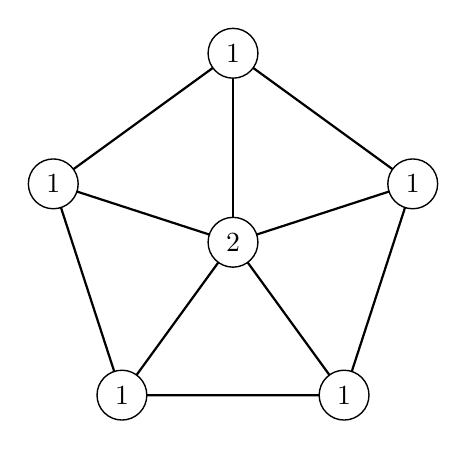
\begin{tikzpicture}[rotate=90,scale=0.6]
            %\draw[help lines] (-5,-5) grid (5,5);
            \GraphInit[vstyle=Simple]
            \SetVertexSimple[Shape=circle, FillColor=black, MinSize=2pt]
            \tikzset{VertexStyle/.append style = {inner sep = \inners, outer sep = \outers}}
            \SetUpVertex[Ldist=3pt]
            \grWheel[prefix=a]{6}
            \AssignVertexLabel{a}{1,1,1,1,1,2}
        \end{tikzpicture}
    \caption{An optimal clique coloring.}
    \label{fig:clique_color}
\end{figure}

Research on the topic is much more recent than what was done for \textsc{vertex coloring}, with the first papers appearing in the early 1990s~\citep{first_clique_color} and interest on the subject rising in the early 2000s.
Even when $k$ is fixed, \textsc{clique $k$-coloring} is known to be $\SiP{2}\text{-}\Complete$, as shown by~\citep{clique_coloring_complexity}, with an $\bigOs{2^n}$ algorithm being proposed by~\citep{clique_color_algorithm}.

As with \textsc{vertex coloring}, \textsc{clique $k$-coloring} has been studied when restricting the input graph to certain graph classes.
\citep{weakly_clique_color} investigated 2-clique-coloring in terms of \tdef{weakly chordal graphs} (graphs free of any hole or anti-hole with more than 4 vertices), giving a series of results for the general case ($\SiP{2}\text{-}\Complete$) and showing that, for some nested subclasses, there are $\NPc$ and $\P$ instances of the problem.
When dealing with \tdef{unichord-free} graphs (graphs that contain no induced cycle with a unique chord), the problem is solvable in polynomial time (\cite{unichord_coloring}).

\tdef{Circular-arc} graphs (intersection graphs of a set of arcs of a circle) are always 3-clique-colorable, with a polynomial time algorithm to determine if the input is 2-clique-colorable \citep{clique_circular_arc}.
When the given graph is \tdef{odd-hole-free}, it is $\SiP{2}\text{-}\Complete$ to decide whether it is 2-clique-colorable or not~\citep{clique_oddhole}.
\citep{clique_coloring_few_p4} give a series of bounds on graphs that, in some sense, contain few $P_4$'s, showing that most them are either 2 or 3-clique-colorable.

For \tdef{planar graphs} (graphs that can be drawn on a plane with no crossing edges), \citep{clique_coloring_planar} show that they are 3-clique-colorable, and \citep{clique_color_perfect_np_complete} present a polynomial time algorithm to decide whether a planar graph is 2-clique-colorable or not.

Some of these classes are subclasses of perfect graphs, and a conjecture suggests that every perfect graph is 3-clique-colorable~\citep{maximal_clique_coloring}.
Also in terms of perfect graphs, it is $\NPc$ to decide whether a perfect graph is 2-clique-colorable (\cite{clique_color_perfect_np_complete}).
\citep{clique_oddhole} also give the observation that every \tdef{strongly perfect graph} (see~\citep{strongly_perfect}) is 2-clique-colorable, a superclass of both chordal graphs and cographs.
For a summary of the mentioned results, please refer to Table~\ref{tab:clique_color_complexity}.

\begin{table}[!htb]
    \centering
    \begin{tabular}{c|c|c}
        \hline
        \hline
        Class            & $\CN{C}$             & Complexity \\
        \hline
        Cograph          & $= 2$                & $\P$\\
        Chordal          & $= 2$                & $\P$\\
        Weakly Chordal   & $\leq 3^*$           & $\SiP{2}\text{-}\Complete^\dag$\\
        Unichord-free    & $\leq 3 $            & $\P$ \\
        Circular-arc     & $\leq 3$             & $\P^\dag$ \\
        Odd-hole-free    & $\leq 3^*$           & $\SiP{2}\text{-}\Complete^\dag$\\
        Few $P_4$'s      & $\leq 2$ or $\leq 3$ & $\P$\\
        Planar           & $\leq 3$             & $\P^\dag$\\
        Perfect          & $\leq 3^*$           & $\NPc^\dag$\\ 
        Strongly Perfect & $= 2$                & $\P$\\
        General case     & Unbounded            & $\SiP{2}\text{-}\Complete$\\
        \hline
        \hline
    \end{tabular}
    \caption{Complexity and bounds for \textsc{clique coloring}. Entries marked with a $*$ are conjectures. $\dag$ indicates results for 2-clique-colorability.}
    \label{tab:clique_color_complexity}
\end{table}

\subsection{Biclique Coloring}
A \tdef{k-biclique-coloring} of $G$ is a $k$-coloring of $G$ such that no maximal biclique of $G$ is entirely contained in a single color class.
We say that $G$ is \tdef{k-biclique-colorable} if $G$ admits a $k$-biclique-coloring.
The smallest integer $k$ such that $G$ is $k$-biclique-colorable is called the \tdef{biclique chromatic number} $\CN{B}(G)$ of $G$.
Much like \textsc{clique coloring}, there is a natural decision problem associated with this coloring variant, which we refer to as \textsc{biclique coloring}.

\problem{biclique coloring}{A graph $G$ and a positive integer $k$.}{Is $G$ $k$-biclique-colorable?}


\begin{figure}[!htb]
    \centering
    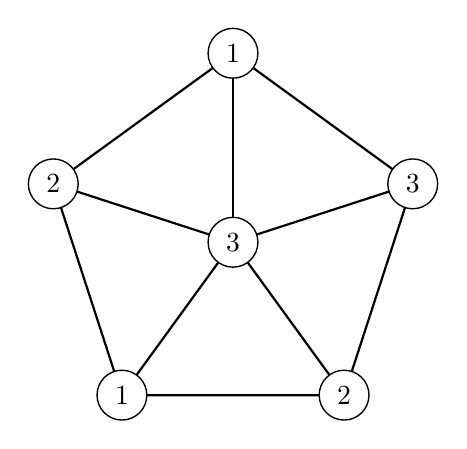
\begin{tikzpicture}[rotate=90,scale=0.6]
            %\draw[help lines] (-5,-5) grid (5,5);
            \GraphInit[vstyle=Simple]
            \SetVertexSimple[Shape=circle, FillColor=black, MinSize=2pt]
            \tikzset{VertexStyle/.append style = {inner sep = \inners, outer sep = \outers}}
            \SetUpVertex[Ldist=3pt]
            \grWheel[prefix=a]{6}
            \AssignVertexLabel{a}{1,2,1,2,3,3}
        \end{tikzpicture}
    \caption{An optimal biclique coloring.}
    \label{fig:biclique_color}
\end{figure}


\textsc{biclique coloring} is an even more recent research topic than \textsc{clique coloring}, with the first results being a $\SiP{2}\text{-}\Cness$ proof due to~\citep{biclique_coloring_complexity} and the confirmation that verifying a solution to the problem is a $\coNP\text{-}\Complete$ task (\cite{biclique_coloring_verification}).

In terms of complexity results, very little is known about \textsc{biclique coloring}.
For unichord-free graphs, \citep{unichord_coloring} give a polynomial time algorithm to compute $\CN{B}$ and show that the biclique chromatic number of unichord-free graphs is either equal to or one greater than the size of the largest true twin class.
\citep{biclique_coloring_verification} present a polynomial time algorithm for powers of cycles and powers of paths.
Finally, \citep{biclique_coloring_complexity} give complexity results for $H$-free graphs, for every $H$ on three vertices, being polynomial for $H \in \{K_3, P_3, \overline{P_3}\}$ and $\NPc$ for $\overline{K_3}$-free graphs;
moreover they show that the problem is $\NPc$ for diamond ($C_4$ plus one chord) free graphs and split graphs, and polynomial for \tdef{threshold graphs} (\{$2K_2,P_4,C_4$\}-free).
We summarize the presented results in Table~\ref{tab:biclique_color_complexity}.

\begin{table}[!htb]
    \centering
    \begin{tabular}{c|c|c}
        \hline
        \hline
        Class            & $\CN{B}$             & Complexity \\
        \hline
        Split            & Unbounded            & $\NPc$\\
        Threshold        & Unbounded            & $\P$\\
        Diamond-free     & Unbounded            & $\NPc$\\
        $C_n^r$          & $\leq 3$             & $\P$\\
        $P_n^r$          & $= 2$                & $\P$\\
        Unichord-free    & Bounded              & $\P$\\
        General case     & Unbounded            & $\SiP{2}\text{-}\Complete$\\
        \hline
        \hline
    \end{tabular}
    \caption{Complexity and bounds for \textsc{biclique coloring}.}
    \label{tab:biclique_color_complexity}
\end{table}

Both \textsc{clique coloring} and \textsc{biclique coloring} are, actually, colorings of the hypergraphs arising from an underlying graph (a coloring of its vertices such that no hyperedge is monochromatic), which is also an $\NPc$ task.
However, in classical hypergraph coloring problems, the hyperedge family is part of the input of the problem and, as such, naively verifying a solution is polynomial on the size of the input.

\subsection{Equitable Coloring}
A $k$-coloring of an $n$ vertex graph is said to be \tdef{equitable} if for every color class $\varphi_i$, $\floor{\frac{n}{k}} \leq |\varphi_i| \leq \ceil{\frac{n}{k}}$ or, equivalently, if for, any two color class $\varphi_i$ and $\varphi_j$, $||\varphi_i| - |\varphi_j|| \leq 1$.
If $G$ admits a proper equitable $k$-coloring, we say that $G$ is \tdef{equitably k-colorable}.
Unlike other coloring variants previously discussed, an equitably $k$-colorable graph is not necessarily equitably $(k+1)$-colorable.

As such, two different parameters are defined: the smallest integer $k$ such that $G$ is equitably $k$-colorable is called the \tdef{equitable chromatic number} $\CN{=}(G)$; the smallest integer $k'$ such that $G$ is equitably $k$-colorable for every $k \geq k'$ is the \textit{equitable chromatic threshold} $\CN{=}^*(G)$ of $G$.

As with the previous coloring problems, we define the \textsc{equitable coloring} decision problem.

\problem{equitable coloring}{A graph $G$ and a positive integer $k$.}{Is $G$ equitably $k$-colorable?}


\begin{figure}[!htb]
    \centering
    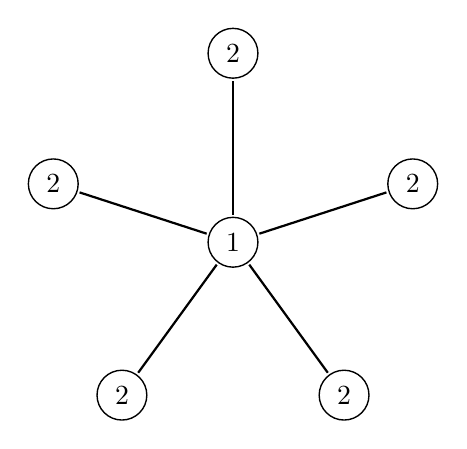
\begin{tikzpicture}
        \begin{scope}[rotate=90,scale=0.6]
            %\draw[help lines] (-5,-5) grid (5,5);
            \GraphInit[vstyle=Normal]
            \SetVertexNormal[Shape=circle]
            \tikzset{VertexStyle/.append style = {inner sep = \inners, outer sep = \outers}}
            \SetVertexNoLabel
            \grStar[prefix=a]{6}
            \AssignVertexLabel{a}{2,2,2,2,2,1}
        \end{scope}
    \end{tikzpicture}
    \hfill
    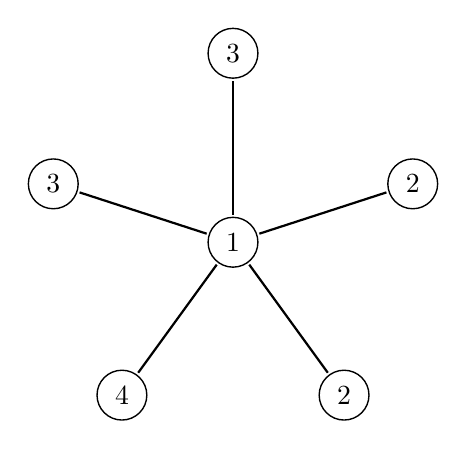
\begin{tikzpicture}
        \begin{scope}[rotate=90,scale=0.6]
            %\draw[help lines] (-5,-5) grid (5,5);
            \GraphInit[vstyle=Normal]
            \SetVertexNormal[Shape=circle]
            \tikzset{VertexStyle/.append style = {inner sep = \inners, outer sep = \outers}}
            \SetVertexNoLabel
            \grStar[prefix=b]{6}
            \AssignVertexLabel{b}{3,3,4,2,2,1}
        \end{scope}
    \end{tikzpicture}
    \hfill
    
    \caption{A proper non-equitable coloring (left) and an equitable coloring (right).}
    \label{fig:eq_color}
\end{figure}


\textsc{equitable coloring} was first discussed by~\citep{first_equitable}, with an intended application for municipal garbage collection, and later in processor task scheduling~\citep{mutual_exclusion_scheduling} and server load balancing~\citep{domain_decomposition}.

Much of the work done over \textsc{equitable coloring} aims to prove an analogue of Brooks' theorem, known as the \tdef{Equitable coloring conjecture} (ECC).
In terms of the equitable chromatic threshold, however, we have the \tdef{Hajnal-Szemerédi theorem}~\citep{hajnal_szmeredi_theorem}.

\begin{conjecture*}[ECC]
    For every connected graph $G$ which is neither a complete graph nor an odd-hole, $\CN{=}(G) \leq \Delta(G)$.
\end{conjecture*}

\begin{theorem*}[Hajnal-Szmerédi Theorem]
    Any graph $G$ is equitably $k$-colorable if $k \geq \Delta(G) + 1$. Equivalently, $\CN{=}^*(G) \leq \Delta(G) + 1$.
\end{theorem*}

\citep{e_delta_cc} suggest that a stronger result than the Hajnal-Szmerédi theorem may be achievable, presenting some classes where the \tdef{Equitable $\Delta$-coloring conjecture} (E$\Delta$CC) holds.
Moreover, they prove that if E$\Delta$CC holds for every regular graph, then it holds for every graph.

\begin{conjecture*}[E$\Delta$CC]
    For every connected graph $G$ which is not a complete graph, an odd-hole nor $K_{2n+1, 2n+1}$, for any $n \geq 1$, $\CN{=}^*(G) \leq \Delta(G)$ holds.
\end{conjecture*}

Quite a lot of effort was put into finding classes where E$\Delta$CC holds, even with the knowledge that only proofs for regular graphs are required.
A result given by~\citep{claw_free_de_werra}, combined with Brooks' Theorem, implies that every claw-free graph is equitably $k$-colorable for every $k \geq \chi(G)$.
Unfortunately, we were unable to verify whether this result is algorithmic and, in the affirmative, the algorithm's complexity.
However, due to the broadness of the class, we believe that, even if it exists, the algorithm has a higher complexity than the ones we describe.

A very extensive survey on the subject was conducted by~\citep{equitable_survey}, where many of the results of the past 50 years were assembled.
Among the many reported results, the E$\Delta$CC is known to hold for:
bipartite graphs (with the obvious exceptions, where the ECC holds),
trees,
split graphs,
planar graphs,
\tdef{outerplanar graphs} (planar graphs with a drawing such that no vertex is within a polygon formed by other vertices),
\tdef{low degeneracy graphs} (graphs such that every subgraph has a vertex with a small degree),
\tdef{Kneser graphs} (complement of the intersection graph of $F \subset 2^{[n]}$, with every set of $F$ containing exactly $k$ elements),
interval graphs,
random graphs and
some forms of graph products.
For the exact results please refer to the survey.

Almost all complexity results for \textsc{equitable coloring} arise from a related problem, known as \textsc{bounded coloring}, an observation given by~\citep{equitable_treewidth}.
A $k$-coloring is said to be \tdef{$l$-bounded} if for every color class $\varphi_i$, $|\varphi_i| \leq l$.
$G$ is \tdef{l-bounded k-colorable} if it admits an $l$-bounded $k$-coloring.

\problem{bounded coloring}{A graph $G$ and two positive integers $l$ and $k$.}{Is $G$ $l$-bounded $k$-colorable?}

\begin{observation*}
    A Graph $G$ with $n$ vertices is $l$-bounded $k$-colorable if and only if $G' = G \cup \overline{K_{lk - n}}$ is equitably $k$-colorable.
\end{observation*}


In terms of computational complexity, however, neither problem was nearly as explored as \textsc{vertex coloring}.
Among the complexity results for \textsc{bounded coloring} and, consequently, \textsc{equitable coloring}, we have polynomial time solvability for split graphs~\citep{equitable_split}, complement of interval graphs~\citep{graph_partitioning1}, forests~\citep{mutual_exclusion_scheduling}, trees~\citep{equitable_trees} and complements of bipartite graphs~\citep{graph_partitioning1}.

For cographs, we have a polynomial time algorithm when $k$ is fixed, otherwise the problem is $\NPc$~\citep{graph_partitioning1}, a situation similar to that of bipartite and interval graphs~\citep{graph_partitioning1}.
A consequence of the hardness result for cographs is that \textsc{equitable coloring} is $\NPc$ for graphs of bounded cliquewidth.

On complements of \tdef{comparability graphs} (graphs representing a valid partial ordering) however, even if we fix $l$, \textsc{bounded coloring} is still $\NPc$~\citep{chain_antichain}.
\citep{colorful_treewidth} show that, when parameterized by treewidth, \textsc{equitable coloring} is $\W[1]\text{-}\Hard$.
Also in terms of treewidth, \citep{equitable_treewidth} give a polynomial time algorithm for graphs of bounded treewidth.
Note that for all of the mentioned classes, \textsc{vertex coloring} is polynomially solvable.

A summary of the known complexities is available in Table~\ref{tab:equitable_complexity}.


\begin{table}[!htb]
    \centering
    \begin{tabular}{l|l|l}
       \hline
       \hline
       Class               &  fixed $k$         & input $k$             \\
       \hline
       Trees                &  $\P$             & $\P$                  \\
       Forests              &  $\P$             & $\P$                  \\
       Bipartite            &  $\NPc$           & $\NPc$                \\
       Co-bipartite         &  $\P$             & $\P$                  \\
       Cographs             &  $\P$             & $\NPc$                \\
       Bounded Cliquewidth  &  ?                & $\NPc$                \\
       Bounded Treewidth    &  $\P$             & $\P$                  \\
       Chordal              &  $\P^*$           & $\NPc$                \\
       Block                &  $\P^*$           & $\NPc^*$              \\
       Split                &  $\P$             & $\P$                  \\
       Interval             &  $\P$             & $\NPc$                \\
       Co-interval          &  $\P$             & $\P$                  \\
       General case         &  $\NPc$           & $\NPc$                \\
       \hline
       \hline
    \end{tabular}
    \caption{Complexity results for \textsc{equitable coloring}. Entries marked with a * are results established in this work.}
    \label{tab:equitable_complexity}
\end{table}


%\chapter{Coloring, Clique, and Biclique Coloring}
\label{ch:coloring}

Some blabla t.

\section{Equitable Coloring}

As previously discussed, \pname{Equitable Coloring} seeks a $k$-coloring of the vertices of an $n$ vertex graph $G$ such that no color is used \say{too many times}. In particular, we want our color classes to have either $\floor{\frac{n}{k}}$ or $\ceil{\frac{n}{k}}$ vertices.
In this section, we present a dynamic programming \XP\ algorithm for \pname{Equitable Coloring}.
Moreover, we show that deciding whether or not a block graph $G$ is colorable with $\omega(G)$ colors is $\NPc$ in the strong sense.
Finally, constructive, polynomial time algorithms for \textsc{equitable coloring} on \{net, claw\}-free block graphs, claw-free block graphs and claw-free chordal graphs are presented.
\section{Hardness of \pname{Equitable Coloring} for subclasses of Chordal Graphs}

\begin{figure}[!tb]
    \centering
    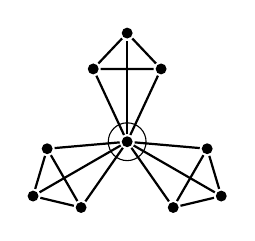
\begin{tikzpicture}[scale=\gscale]
        %\draw[help lines] (-5,-5) grid (5,5);
        \GraphInit[unit=3,vstyle=Normal]
        \SetVertexNormal[Shape=circle, FillColor=black, MinSize=2pt]
        \tikzset{VertexStyle/.append style = {inner sep = \inners, outer sep = \outers}}
        \SetVertexNoLabel
        \Vertex[x=0,y=0,L={y}, Lpos=270, LabelOut, Ldist=3pt]{y}
        \draw[] (0,0) circle (0.4cm);
        \Vertex[a=-5, d=1.7cm]{x11}
        \Vertex[a=-30, d=2.3cm]{x12}
        \Vertex[a=-55, d=1.7cm]{x13}
        
        \Vertex[a=115, d=1.7cm]{x21}
        \Vertex[a=90, d=2.3cm]{x22}
        \Vertex[a=65, d=1.7cm]{x23}
        
        \Vertex[a=235, d=1.7cm]{x31}
        \Vertex[a=210, d=2.3cm]{x32}
        \Vertex[a=185, d=1.7cm]{x33}
        
        \foreach \x in {1,2,3}
            \foreach \y in {1,2,3}
                \Edge(y)(x\x\y);
        
        \Edge(x11)(x12)
        \Edge(x11)(x13)
        \Edge(x12)(x13)
        
        
        \Edge(x21)(x22)
        \Edge(x21)(x23)
        \Edge(x22)(x23)
        
        
        \Edge(x31)(x32)
        \Edge(x31)(x33)
        \Edge(x32)(x33)
        
        
    \end{tikzpicture}
    \hfill
    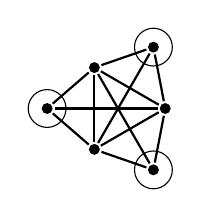
\begin{tikzpicture}[scale=\gscale]
        \GraphInit[unit=3,vstyle=Normal]
        \SetVertexNormal[Shape=circle, FillColor=black, MinSize=2pt]
        \tikzset{VertexStyle/.append style = {inner sep = \inners, outer sep = \outers}}
        \SetVertexNoLabel
        \grComplete[RA=1]{3}
        \Vertex[a=60,d=1.5]{x}
        \Vertex[a=180,d=1.5]{y}
        \Vertex[a=300,d=1.5]{z}
        \draw[] (60:1.5) circle (0.4cm);
        \draw[] (180:1.5) circle (0.4cm);
        \draw[] (300:1.5) circle (0.4cm);
        
        \Edge(x)(a0)
        \Edge(x)(a1)
        \Edge(x)(a2)
        
        \Edge(y)(a0)
        \Edge(y)(a1)
        \Edge(y)(a2)
        
        \Edge(z)(a0)
        \Edge(z)(a1)
        \Edge(z)(a2)
        
    \end{tikzpicture}
    \hfill
    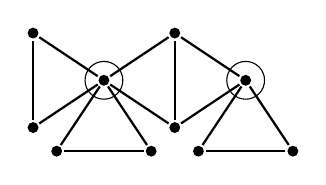
\begin{tikzpicture}[scale=\gscale]
        \GraphInit[unit=3,vstyle=Normal]
        \SetVertexNormal[Shape=circle, FillColor=black, MinSize=2pt]
        \tikzset{VertexStyle/.append style = {inner sep = \inners, outer sep = \outers}}
        \SetVertexNoLabel
        \Vertex[x=0,y=0]{y1}
        
        \draw[] (0,0) circle (0.4cm);
        
        \Vertex[x=3,y=0]{y2}
        
        \draw[] (3,0) circle (0.4cm);
        
        \begin{scope}[shift={(1.5cm,0)}, rotate=-90]
            \grComplete[RA=1, prefix=a]{2}
        \end{scope}
        
        \begin{scope}[shift={(0cm,-1.5cm)}]
            \grComplete[RA=1, prefix=c]{2}
        \end{scope}
        
        \begin{scope}[shift={(-1.5cm,0)}, rotate=-90]
            \grComplete[RA=1, prefix=b]{2}
        \end{scope}
        
        \begin{scope}[shift={(3cm,-1.5cm)}]
            \grComplete[RA=1, prefix=d]{2}
        \end{scope}
        
        \Edges(a0,y1,a1)
        \Edges(b0,y1,b1)
        \Edges(c0,y1,c1)
        
        \Edges(a0,y2,a1)
        \Edges(d0,y2,d1)
        
        
    \end{tikzpicture}
    \hfill
    
    \caption{A $(2,4)$-flower, a $(2,4)$-antiflower, and a $(2,2)$-trem.}
    \label{fig:flower}
\end{figure}

\begin{figure}[!tb]
    \centering
    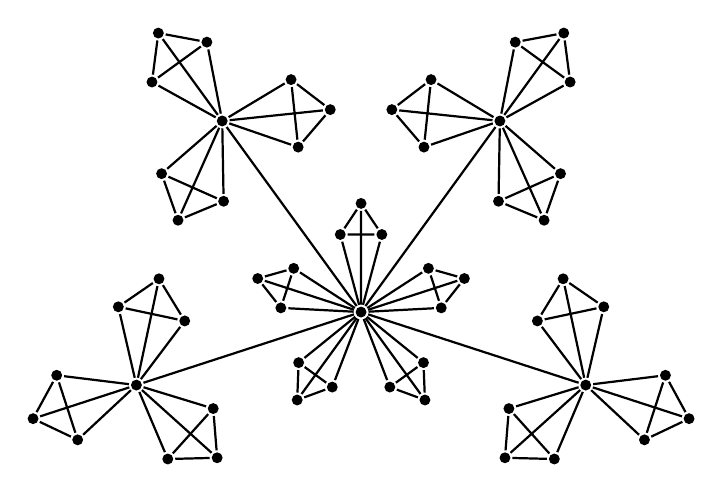
\begin{tikzpicture}[scale=\gscale]
            %\draw[help lines] (-8,-8) grid (8,8);
        \begin{scope}[rotate=36,shift={(0cm, 5cm)}]
            \GraphInit[unit=3,vstyle=Normal]
            \SetVertexNormal[Shape=circle, FillColor=black, MinSize=2pt]
            \tikzset{VertexStyle/.append style = {inner sep = \inners, outer sep = \outers}}
            \SetVertexNoLabel
            \Vertex[Math, x=0,y=0,L={y_1}, Lpos=290, LabelOut, Ldist=3pt]{1y}
            \Vertex[a=-5, d=1.7cm]{1x11}
            \Vertex[a=-30, d=2.3cm]{1x12}
            \Vertex[a=-55, d=1.7cm]{1x13}
            
            \Vertex[a=115, d=1.7cm]{1x21}
            \Vertex[a=90, d=2.3cm]{1x22}
            \Vertex[a=65, d=1.7cm]{1x23}
            
            \Vertex[a=235, d=1.7cm]{1x31}
            \Vertex[a=210, d=2.3cm]{1x32}
            \Vertex[a=185, d=1.7cm]{1x33}
            
            \foreach \x in {1,2,3}
                \foreach \y in {1,2,3}
                    \Edge(1y)(1x\x\y);
            
            \Edge(1x11)(1x12)
            \Edge(1x11)(1x13)
            \Edge(1x12)(1x13)
            
            
            \Edge(1x21)(1x22)
            \Edge(1x21)(1x23)
            \Edge(1x22)(1x23)
            
            
            \Edge(1x31)(1x32)
            \Edge(1x31)(1x33)
            \Edge(1x32)(1x33)
        \end{scope}
        \begin{scope}[rotate=-36,shift={(0cm, 5cm)}]
            \GraphInit[unit=3,vstyle=Normal]
            \SetVertexNormal[Shape=circle, FillColor=black, MinSize=2pt]
            \tikzset{VertexStyle/.append style = {inner sep = \inners, outer sep = \outers}}
            \SetVertexNoLabel
            \Vertex[Math, x=0,y=0,L={y_1}, Lpos=290, LabelOut, Ldist=3pt]{2y}
            \Vertex[a=-5, d=1.7cm]{2x11}
            \Vertex[a=-30, d=2.3cm]{2x12}
            \Vertex[a=-55, d=1.7cm]{2x13}
            
            \Vertex[a=115, d=1.7cm]{2x21}
            \Vertex[a=90, d=2.3cm]{2x22}
            \Vertex[a=65, d=1.7cm]{2x23}
            
            \Vertex[a=235, d=1.7cm]{2x31}
            \Vertex[a=210, d=2.3cm]{2x32}
            \Vertex[a=185, d=1.7cm]{2x33}
            
            \foreach \x in {1,2,3}
                \foreach \y in {1,2,3}
                    \Edge(2y)(2x\x\y);
            
            \Edge(2x11)(2x12)
            \Edge(2x11)(2x13)
            \Edge(2x12)(2x13)
            
            
            \Edge(2x21)(2x22)
            \Edge(2x21)(2x23)
            \Edge(2x22)(2x23)
            
            
            \Edge(2x31)(2x32)
            \Edge(2x31)(2x33)
            \Edge(2x32)(2x33)
        \end{scope}
        \begin{scope}[rotate=-108,shift={(0cm, 5cm)}]
            \GraphInit[unit=3,vstyle=Normal]
            \SetVertexNormal[Shape=circle, FillColor=black, MinSize=2pt]
            \tikzset{VertexStyle/.append style = {inner sep = \inners, outer sep = \outers}}
            \SetVertexNoLabel
            \Vertex[Math, x=0,y=0,L={y_1}, Lpos=290, LabelOut, Ldist=3pt]{3y}
            \Vertex[a=-5, d=1.7cm]{3x11}
            \Vertex[a=-30, d=2.3cm]{3x12}
            \Vertex[a=-55, d=1.7cm]{3x13}
            
            \Vertex[a=115, d=1.7cm]{3x21}
            \Vertex[a=90, d=2.3cm]{3x22}
            \Vertex[a=65, d=1.7cm]{3x23}
            
            \Vertex[a=235, d=1.7cm]{3x31}
            \Vertex[a=210, d=2.3cm]{3x32}
            \Vertex[a=185, d=1.7cm]{3x33}
            
            \foreach \x in {1,2,3}
                \foreach \y in {1,2,3}
                    \Edge(3y)(3x\x\y);
            
            \Edge(3x11)(3x12)
            \Edge(3x11)(3x13)
            \Edge(3x12)(3x13)
            
            
            \Edge(3x21)(3x22)
            \Edge(3x21)(3x23)
            \Edge(3x22)(3x23)
            
            
            \Edge(3x31)(3x32)
            \Edge(3x31)(3x33)
            \Edge(3x32)(3x33)
        \end{scope}
        \begin{scope}[rotate=108,shift={(0cm, 5cm)}]
            \GraphInit[unit=3,vstyle=Normal]
            \SetVertexNormal[Shape=circle, FillColor=black, MinSize=2pt]
            \tikzset{VertexStyle/.append style = {inner sep = \inners, outer sep = \outers}}
            \SetVertexNoLabel
            \Vertex[Math, x=0,y=0,L={y_1}, Lpos=290, LabelOut, Ldist=3pt]{4y}
            \Vertex[a=-5, d=1.7cm]{4x11}
            \Vertex[a=-30, d=2.3cm]{4x12}
            \Vertex[a=-55, d=1.7cm]{4x13}
            
            \Vertex[a=115, d=1.7cm]{4x21}
            \Vertex[a=90, d=2.3cm]{4x22}
            \Vertex[a=65, d=1.7cm]{4x23}
            
            \Vertex[a=235, d=1.7cm]{4x31}
            \Vertex[a=210, d=2.3cm]{4x32}
            \Vertex[a=185, d=1.7cm]{4x33}
            
            \foreach \x in {1,2,3}
                \foreach \y in {1,2,3}
                    \Edge(4y)(4x\x\y);
            
            \Edge(4x11)(4x12)
            \Edge(4x11)(4x13)
            \Edge(4x12)(4x13)
            
            
            \Edge(4x21)(4x22)
            \Edge(4x21)(4x23)
            \Edge(4x22)(4x23)
            
            
            \Edge(4x31)(4x32)
            \Edge(4x31)(4x33)
            \Edge(4x32)(4x33)
        \end{scope}
        \begin{scope}[rotate=120,shift={(0cm, 0cm)}]
            \GraphInit[unit=3,vstyle=Normal]
            \SetVertexNormal[Shape=circle, FillColor=black, MinSize=2pt]
            \tikzset{VertexStyle/.append style = {inner sep = \inners, outer sep = \outers}}
            \SetVertexNoLabel
            \Vertex[Math, x=0,y=0,L={y_1}, Lpos=290, LabelOut, Ldist=3pt]{0y}
            \Vertex[a=-15, d=1.7cm]{0x11}
            \Vertex[a=-30, d=2.3cm]{0x12}
            \Vertex[a=-45, d=1.7cm]{0x13}
            
            \Vertex[a=-87, d=1.7cm]{0x21}
            \Vertex[a=-102, d=2.3cm]{0x22}
            \Vertex[a=-117, d=1.7cm]{0x23}
            
            \Vertex[a=-159, d=1.7cm]{0x31}
            \Vertex[a=-174, d=2.3cm]{0x32}
            \Vertex[a=-189, d=1.7cm]{0x33}
            
            \Vertex[a=-231, d=1.7cm]{0x41}
            \Vertex[a=-246, d=2.3cm]{0x42}
            \Vertex[a=-261, d=1.7cm]{0x43}
            
            \Vertex[a=-303, d=1.7cm]{0x51}
            \Vertex[a=-318, d=2.3cm]{0x52}
            \Vertex[a=-333, d=1.7cm]{0x53}
            
            
            \foreach \x in {1,2,3,4,5}
                \foreach \y in {1,2,3}
                    \Edge(0y)(0x\x\y);
                    
                    \Edge(0x11)(0x11)
            \Edge(0x11)(0x12)
            \Edge(0x11)(0x13)
            \Edge(0x12)(0x12)
            \Edge(0x12)(0x13)
            \Edge(0x13)(0x13)
            \Edge(0x21)(0x21)
            \Edge(0x21)(0x22)
            \Edge(0x21)(0x23)
            \Edge(0x22)(0x22)
            \Edge(0x22)(0x23)
            \Edge(0x23)(0x23)
            \Edge(0x31)(0x31)
            \Edge(0x31)(0x32)
            \Edge(0x31)(0x33)
            \Edge(0x32)(0x32)
            \Edge(0x32)(0x33)
            \Edge(0x33)(0x33)
            \Edge(0x41)(0x41)
            \Edge(0x41)(0x42)
            \Edge(0x41)(0x43)
            \Edge(0x42)(0x42)
            \Edge(0x42)(0x43)
            \Edge(0x43)(0x43)
            \Edge(0x51)(0x51)
            \Edge(0x51)(0x52)
            \Edge(0x51)(0x53)
            \Edge(0x52)(0x52)
            \Edge(0x52)(0x53)
            \Edge(0x53)(0x53)
            
        \end{scope}
        \Edge(0y)(1y)
        \Edge(0y)(2y)
        \Edge(0y)(3y)
        \Edge(0y)(4y)
        
        
    \end{tikzpicture}
    
    \caption{\textsc{equitable coloring} instance built on Theorem~\ref{thm:blocks} corresponding to the \pname{Bin Packing} instance $A = \{2,2,2,2\}$, $k=3$ and $B = 4$.}
    \label{fig:super_flower}
\end{figure}

All of our reductions involve the \pname{Bin Packing} problem, which is $\NPH$ in the strong sense~\citep{garey_johnson} and $\W[1]$-$\Hard$ when parameterized by the number of bins~\citep{bin_packing_w1}.
In the general case, the problem is defined as: given a set of positive integers $A = \{a_1, \dots, a_n\}$, called \textit{items}, and two integers $k$ and $B$, can we partition $A$ into $k$ \emph{bins} such that the sum of the elements of each bin is at most $B$?
We shall use a version of \pname{Bin Packing} where each bin sums \emph{exactly} to~$B$.
This second version is equivalent to the first, even from the parameterized point of view; it suffices to add~$kB - \sum_{j \in [n]} a_j$ unitary items to~$A$.
For simplicity, by \pname{Bin Packing} we shall refer to the second version, which we formalize as follows.

\pproblem{bin-packing}{A set of $n$ items $A$ and a bin capacity $B$.}{The number of bins $k$.}{Is there a $k$-partition $\varphi$ of $A$ such that, $\forall i \in [k]$, $\sum_{a_j \in \varphi_i} a_j = B$?}

The idea for the following reductions is to build one gadget for each item~$a_j$ of the given \pname{Bin Packing} instance, perform their disjoint union, and equitably $k$-color the resulting graph.
The color given to the circled vertices in Figure~\ref{fig:flower} control the bin to which the corresponding item belongs to.
Each reduction uses only one of the three gadget types.
Since every gadget is a chordal graph, their treewidth is precisely the size of the largest clique minus one, that is, $k$, which is also the number of desired colors for the built instance of \textsc{equitable coloring}.

\subsubsection{Disjoint union of Split Graphs}

\begin{definition}
    An $(a,k)$-antiflower is the graph $F_-(a,k) = K_{k-1} \oplus \left(\bigcup_{i \in [a+1]} K_1\right)$, that is, it is the graph obtained after performing the disjoint union of $a+1$ $K_1$'s followed by the join with $K_{k-1}$.
\end{definition}

\begin{theorem}
    \label{thm:dis_split}
    \textsc{equitable coloring} of the disjoint union of split graphs parameterized by the number of colors is $\W[1]$-$\Hard$.
\end{theorem}
\begin{proof}
    Let $\langle A,k,B\rangle$ be an instance of \pname{Bin Packing} and $G$ a graph such that~$G = \bigcup_{j \in [n]} F_-(a_j,k)$.
    Note that $|V(G)| = \sum_{j \in [n]} |F_-(a_j, k)| = \sum_{j \in [n]} k + a_j = nk + kB$.
    Therefore, in any equitable $k$-coloring of~$G$, each color class has~$n + B$ vertices.
    Define~$F_j = F_-(a_j,k)$ and let~$C_j$ be the corresponding $K_{k-1}$.
    We show that there is an equitable~$k$-coloring~$\psi$ of~$G$ if and only if~$\varphi = \langle A,k,B\rangle$ is a $\YES$ instance of \pname{Bin Packing}.
    
    Let~$\varphi$ be a solution to \pname{Bin Packing}.
    For each~$a_j \in A$, we do $\psi(C_j) = [k] \setminus \{i\}$ if $a_j \in \varphi_i$.
    We color each vertex of the independent set of~$F_{j}$ with~$i$ and note that all remaining possible proper colorings of the gadget use each color the same number of times.
    Thus, $|\psi_i| = \sum_{j \mid a_j \in \varphi_i} (a_j + 1) + \sum_{j \mid a_j \notin \varphi_i} 1 = \sum_{j \mid a_j \in \varphi_i} (a_j + 1) + \sum_{j \in [n]} 1 - \sum_{j \mid a_j \in \varphi_i} 1 = n + B$.
    
    Now, let~$\psi$ be an equitable $k$-coloring of~$G$.
    Note that~$|\psi_i| = n+B$ and that the independent set of an antiflower is monochromatic.
    For each $j \in [n]$, $a_j \in \varphi_i$ if $i \notin \psi(C_j)$.
    That is, $n + B = |\psi_i| = \sum_{j \mid i \notin C_j} (a_j + 1) + \sum_{j \mid i \in C_j} 1 = \sum_{j \mid i \notin C_j} (a_j + 1) + \sum_{j \in [n]} 1 - \sum_{j \mid i \notin C_j} 1 = \sum_{j \mid i \notin C_j} a_j + n$, from which we conclude that $\sum_{j \mid i \notin C_j} a_j = B$.
\end{proof}

\subsubsection{Block Graphs}

We now proceed to the parameterized complexity of block graphs.
Conceptually, the proof follows a similar argumentation as the one developed in Theorem~\ref{thm:dis_split}; in fact, we are able to show that even restricting the problem to graphs of diameter at least four is not enough to develop an $\FPT$ algorithm, unless $\FPT = \W[1]$.
 
\begin{definition}
    An $(a,k)$-flower is the graph $F(a,k) = K_1 \oplus \left(\bigcup_{i \in [a+1]} K_{k-1}\right)$, that is, it is obtained from the union of $a+1$ cliques of size $k-1$ followed by a join with $K_1$.
\end{definition}

\begin{theorem}
    \label{thm:blocks}
    \textsc{equitable coloring} of block graphs of diameter at least four parameterized by the number of colors and treewidth is $\W[1]$-$\Hard$. 
\end{theorem}

\begin{tproof}
    Let $\langle A,k,B\rangle$ be an instance of \pname{Bin Packing}, $\forall k \in [n]$, $F_j = F(a_j, k+1)$, $F_0 = F(B, k+1)$ and, for $j \in \{0\} \cup [n]$, let $y_j$ be the universal vertex of $F_j$.
    Define a graph $G$ such that $V(G) = V\left(\bigcup_{j \in \{0\} \cup [n]} V(F_j)\right)$ and $E(G) = \{y_0y_j \mid j \in [n]\} \cup E\left(\bigcup_{j \in \{0\} \cup [n]} E(F_j)\right)$.
    Looking at Figure~\ref{fig:super_flower}, it is easy to see that any minimum path between a non-universal vertex of $F_a$ and a non-universal vertex of $F_b$, $a \neq b \neq 0$ has length four.
    We show that $\langle A,k,B\rangle$ is an $\YES$ instance if and only if $G$ is equitably $(k+1)$-colorable.
    \begin{align*}
        |V(G)| &= |V(F_0)| + \sum_{j \in [n]} |V(F_j)| &= &k(B + 1) + 1 + \sum_{j \in [n]} \left(1 + k(a_j + 1)\right)\\
               &= kB + k + n + k^2B + kn + 1           &= &(k+1)(kB + n + 1)\\
    \end{align*}
    
    Given a $k$-partition $\varphi$ of $A$ that solves our instance of \pname{Bin Packing}, we construct a coloring $\psi$ of $G$ such that $\psi(y_j) = i$ if $a_j \in \varphi_i$ and $\psi(y_0) = k+1$.
    Using a similar argument to the previous theorem, after coloring each $y_j$, the remaining vertices of $G$ are automatically colored.
    For $\psi_{k+1}$, note that $|\psi_{k+1}| = 1 + \sum_{j \in [n]} (a_j + 1) = kB + n + 1 = \frac{|V(G)|}{k+1}$.
    It remains to prove that every other color class $\psi_i$ also has $\frac{|V(G)|}{k+1}$ vertices.
    
    \begin{align*}
        |\psi_i| &= B + 1 + \sum_{j \mid y_j \notin \psi_i} (a_j + 1) + \sum_{j \mid y_j \in \psi_i} 1 &= &B + 1 + \sum_{j \in [n]} (a_j + 1) - \sum_{j \mid y_j \in \psi_i} a_j\\
                 &= B + 1 + kB + n - B &= &kB + n + 1\\
    \end{align*}
    
    For the converse we take an equitable $(k+1)$-coloring of $G$ and suppose, without loss of generality, that $\psi(y_0) = k+1$ and, consequently, for every other $y_i$, $\psi(y_i) \neq k+1$.
    To build our $k$-partition $\varphi$ of $A$, we say that $a_j \in \varphi_i$ if $\psi(y_j) = i$.
    The following equalities show that $\sum_{a_j \in \varphi_i} a_j = B$ for every $i$, completing the proof.
    
    \begin{align*}
        |\psi_i|  &= B + 1 + \sum_{j \mid y_j \in \psi_i} 1 + \sum_{j \mid y_j \notin \psi_i} (a_j + 1) &= &B + 1 + \sum_{j \in [n]} (a_j + 1) - \sum_{j \mid y_j \in \psi_i} a_j \\
        kB + n + 1 &= B + 1 + kB + n - \sum_{j \mid y_j \in \psi_i} a_j &\Rightarrow &B =  \sum_{j \mid y_j \in \psi_i} a_j
    \end{align*}
\end{tproof}

\subsubsection{Interval Graphs without some induced stars}


\begin{definition}
    Let $\mathcal{Q} = \{Q_1, Q_1', \dots, Q_a, Q_a'\}$ be a family of cliques such that $Q_i \simeq Q_i' \simeq K_{k-1}$ and $Y = \{y_1, \dots, y_a\}$ be a set of vertices.
    An $(a,k)$-trem is the graph $H(a,k)$ where $V\left(H(a,k)\right) = \mathcal{Q} \cup Y$ and $E\left(H(a,k)\right) = E\left(\bigcup_{i \in [a]} (Q_i \cup Q_i') \oplus y_i\right) \cup E\left(\bigcup_{i \in [a-1]} y_i \oplus Q_{i+1}\right)$.
\end{definition}

\begin{theorem}
    \label{thm:chordal_w1_hard}
    \pname{Equitable Coloring} of $K_{1,4}$ free interval graphs parameterized by treewidth, maximum number of colors and maximum degree is $\W[1]$-$\Hard$.
\end{theorem}

\begin{tproof}
    Once again, let $\langle A,k,B\rangle$ be an instance of \pname{Bin Packing}, define $\forall j \in [n]$, $H_j = H(a_j, k)$ and let $Y_j$ be the set of cut-vertices of $H_j$.
    The graph $G$ is defined as $G = \bigcup_{j \in [n]} V(H_j)$.
    By the definition of an $(a,k)$-trem, we note that the vertices with largest degree are the ones contained in $Y_j \setminus \{y_a\}$, which have degree equal to $3(k-1)$.
    We show that $\langle A,k,B\rangle$ is an $\YES$ instance if and only if $G$ is equitably $k$-colorable, but first note that $|V(G)| = \sum_{j \in [n]} |V(H_j)| = \sum_{j \in [n]} a_j + 2a_j(k-1) = kB + 2(k-1)kB = k(2kB - B)$.
    
    Given a $k$-partition $\varphi$ of $A$ that solves our instance of \pname{Bin Packing}, we construct a coloring $\psi$ of $G$ such that, for each $y \in Y_j$, $\psi(y) = i$ if and only if $a_j \in \varphi_i$.
    Using a similar argument to the other theorems, after coloring each $Y_j$, the remaining vertices of $G$ are automatically colored, and we have  $|\psi_i| = \sum_{j \in \varphi_i} a_j + \sum_{j \notin \varphi_i} 2a_j = B + 2(k-1)B = 2kB - B$.
    
    For the converse we take an equitable $k$-coloring of $G$ and observe that, for every $j \in [n]$, $|\psi(Y_j)| = 1$.
    As such, to build our $k$-partition $\varphi$ of $A$, we say that $a_j \in \varphi_i$ if and only if $\psi(Y_j) = \{i\}$.
    Thus, since $|\psi| = 2kB - B$, we have that $2kB - B = \sum_{j \in \varphi_i} a_j + \sum_{j \notin \varphi_i} 2a_j = \sum_{j \in [n]} a_j - \sum_{j \in \varphi_i} a_j = 2kB - \sum_{j \in \varphi_i} a_j$, from which we conclude that $B = \sum_{j \in \varphi_i} a_j$.
\end{tproof}
\section{Exact algorithms for \pname{Equitable Coloring}}

\subsection{Chordal graphs}

In this section we will make heavy use of the clique tree $\mathcal{T}(G) = (\mathcal{Q}, F)$ of our chordal graph $G$, which we denote by $\mathcal{T}$ for simplicity.
We also assume that $\mathcal{Q} = \{Q_1, \dots, Q_r\}$, $|V(G)| = n$, that $\mathcal{T}$ is rooted at $Q_1$ and that $T_i$ is the subtree of $\mathcal{T}$ rooted at bag $Q_i$.

Our dynamic programming algorithm explores the separability structure inherent to chordal graphs, embodied by the clique tree, to combine every coloring of a subtree that may yield an equitable coloring of the whole graph.
To do so, we must keep track of which bag, say $Q_i$, we are currently exploring and which colors have been used at the separator between $Q_i$ and $\mathcal{T} \setminus Q_i$.

A \tdef{$k$-color counter}, or simply a \tdef{counter} for an $n$ vertex graph is an element $X \in \left(\left[\ceil{\frac{n}{k}}\right] \cup \{0\}\right)^k$, that is, the $k$-th Cartesian power of $\left[\ceil{\frac{n}{k}}\right] \cup \{0\}$.
A counter $X$ is \tdef{equitable} if for every $x_i, x_j \in X$, $|x_i - x_j| \leq 1$.
For simplicity, denote $S(n,k) = \left[\ceil{\frac{n}{k}}\right] \cup \{0\}$.
The \tdef{sum} of two counters $X,Y$ is defined as $X + Y = (x_1 + y_1, \dots, x_k + y_k)$.
We also define the sum of two families $\mathcal{X}, \mathcal{Y}$ of counters as $\mathcal{Z} = \mathcal{X} + \mathcal{Y} = \left\{X + Y \in S(n,k)^k \mid X \in \mathcal{X}, Y \in \mathcal{Y} \right\}$, that is, the sum of all pairs of elements from each family that belong to $S(n,k)^k$.

\begin{observation}
    \label{obs:counter_bound}
    If $\mathcal{X}, \mathcal{Y} \subseteq S(n,k)^k$ and $\mathcal{Z} = \mathcal{X} + \mathcal{Y}$, $|\mathcal{Z}| \leq |S(n,k)|^k $.
\end{observation}

\begin{theorem}
    \label{thm:chordal_exp}
    There is an $\bigO{n^{2k+2}}$ time algorithm for \pname{Equitable Coloring} on chordal graphs where $k$ is the maximum number of colors.
\end{theorem}

\begin{tproof}
    Let $G$ be the input chordal graph of order $n$ and $\mathcal{T}$ its clique tree, rooted at bag $Q_1$. Moreover, we assume that $k \geq \omega(G)$, otherwise the answer is trivially $\NOi$.
    
    For a bag $Q$, denote by $p(Q)$ the parent clique of $Q$ on $\mathcal{T}$, $I(Q) = Q \cap p(Q)$ and by $U(Q) = Q \setminus p(Q)$ the set of vertices that first appeared on the path between $Q$ and the root $Q_1$ (if $Q = Q_1$, $U(Q) = Q$).
    
    Given $Q$ and a list of available colors $L$, define $\Pi(Q,L)$ as the set of all colorings of $U(Q)$ using only the colors of $L$, $\beta(Q,L,\pi)$ the list of colors used by $L$ and $\pi$ to color $I(Q)$ and $Y(Q,\pi)$ as the counter where $y_i = 1$ if and only if some vertex of $U(Q)$ was colored with color $i$ in $\pi$.
    
    We define our dynamic programming state $f(Q_i, L)$ as all colorings of $T_i$ conditioned to the fact that $I(Q_i)$ was colored with $L$. Intuitively, we will try every possible coloring $\pi$ of $U(Q)$ and combine the solutions of each bag adjacent to $Q_i$ given the colors used by $\pi$ and $L$. Finally, there will be an equitable $k$-coloring of $G$ if there is an equitable counter in $f(Q_1, \emptyset)$.
    
    \begin{equation*}
        f(Q_i, L) = \bigcup_{\pi \in \Pi(Q_i, [k] \setminus L)} \left(Y(Q_i, \pi) + \sum_{Q_j \in N_{T_i}(Q_i)} f(Q_j, \beta(Q_j, L, \pi))\right)
    \end{equation*}
    
    To prove the correctness of our algorithm, we will use induction on the size of $\mathcal{T}$.
    For the base case, where $|V(\mathcal{T})| = 1$, trivially, any proper coloring of $G$ will be equitable.
    
    For the general case, suppose that $Q_i$ has at least one child, say $Q_j$.
    Inductively, for any list of colors $R$, $f(Q_j, R)$ holds every proper coloring of $T_j \setminus I(Q_j)$, given that $I(Q_j)$ was colored with $R$.
    In particular, for every $\pi \in \Pi(Q_i, [k] \setminus L)$ we have this guarantee.
    Note that, for each pair of children $Q_j, Q_l$ of $Q_i$, their solutions are completely independent because $Q_j \cap Q_l \subseteq Q_i$ (clique tree property) and $Q_i$ is entirely colored by $\pi$ and $L$.
    This implies that no vertex was counted more than once on each counter, since their color is chosen exactly once for each possible $\pi$.
    Therefore, since the problems are independent for each child of $Q_i$, $\mathcal{Z}(\pi) = \sum_{Q_j \in N_{T_i}(Q_i)} f(Q_j, \beta(Q_j, L, \pi))$ combines every possible coloring of the children of $Q_i$ and $\mathcal{Z}(\pi) + Y(Q_i, \pi)$ is the family of all colorings of $T_i$, given that $Q_i$ was colored with $\pi$ and $L$.
    Finally, $\bigcup_{\pi \in \Pi(Q_i, [k] \setminus L)} Y(Q, \pi) + Z(\pi)$ tries every possible coloring $\pi$ of $Q_i$, guaranteeing that $f(Q_i, L)$ has every possible coloring of $T_i$, given that $I(Q_i)$ used $L$.
    Since $f(Q_i, L)$ has every coloring of $\mathcal{T_i}$ given $L$, $G$ will be equitably $k$-colorable if and only if there is an equitable counter at $f(Q_1, \emptyset)$.
    
    In terms of complexity analysis, we first note that each sum of two counter families $\mathcal{X},\mathcal{Y}$ takes $\bigO{|\mathcal{X}||\mathcal{Y}|}$.
    However, due to Observation~\ref{obs:counter_bound}, the size of $\mathcal{X} + \mathcal{Y}$ is at most $|S(N,k)|^k$ and, therefore, $\sum_{Q_j \in N_{T_i}(Q_i)} f(Q_j, \beta(Q_j, L, \pi))$ takes at most $\bigO{n|S(n,k)|^{2k}} = \bigO{n \left(\ceil{\frac{n}{k}} + 1\right)^{2k}}$ time; moreover, the addition of $Y(Q_i, \pi)$ to $\mathcal{Z}(\pi)$, by the same argument, is $\bigO{|S(n,k)|^k}$.
    
    For the outermost union, we have $\bigO{k!}$ possible colorings $\pi$ for $U(Q_i)$, which implies that computing each $f(Q_i, L)$ takes $\bigO{k!n\left(\ceil{\frac{n}{k}} + 1\right)^{2k}}$ time.
    Since we have $r \leq n$ bags and $k!$ possible lists, there are $\bigO{nk!}$ states, therefore the total complexity of our dynamic programming algorithm is $\bigO{k!^2n^2\left(\ceil{\frac{n}{k}} + 1\right)^{2k}} = \bigO{n^{2k + 2}}$.
\end{tproof}

\begin{corollary}
    \pname{Equitable Coloring} of chordal graphs parameterized by the number of colors is in $\XP$.
\end{corollary}

As shown by Theorem~\ref{thm:chordal_w1_hard}, \pname{Equitable Coloring} of $K_{1,4}$-free interval graphs is \W[1]-\Hard when parameterized by treewidth, maximum number of colors and maximum degree.
The construction of the hard instance, however, has a massive amount of copies of the claw ($K_{1,3}$); determining the complexity of the problem for the class of claw-free chordal graphs is, therefore, a direct question. 
Before answering it, we require a bit more of notation.
Given a partial $k$-coloring $\varphi$ of $G$, let $G[\varphi]$ denote the subgraph of $G$ induced by the vertices colored with $\varphi$, define $\varphi_-$ as the set of colors used $\floor{|V(G[\varphi])|/k}$ times in $\varphi$ and $\varphi_+$ the remaining colors.
If $k$ divides $|V(G[\varphi])|$, we say that $\varphi_+ = \emptyset$.
Our goal is to color $G$ one maximal clique (say $Q$) at a time and keep the invariant that the new vertices introduced by $Q$ can be colored with a subset of the elements of $L_-$.
To do so, we rely on the fact that, for claw-free graphs, the maximal connected components of the subgraph induced by any two colors form either cycles, which cannot happen since $G$ is chordal, or paths.
By carefully choosing which colors to look at, we find odd length paths that can be greedily recolored to restore our invariant.

\begin{lemma}
    \label{lem:claw_free_chordal}
    There is an $\bigO{n^2}$-time algorithm to equitably $k$-color a claw-free chordal graph or determine that no such coloring exists.
\end{lemma}

\begin{proof}
    We proceed by induction on the number $n$ of vertices of $G$, and show that $G$ is equitably $k$-colorable if and only if its maximum clique has size at most $k$.
    The case $n = 1$ is trivial.
    For general $n$, take one of the leaves of the clique tree of $G$, say $Q$, a simplicial vertex $v \in Q$ and define $G' = G \setminus \{v\}$.
    By the inductive hypothesis, there is an equitable $k$-coloring of $G'$ if and only if $k \geq \omega(G')$.
    If $k < \omega(G')$ or $k < |Q|$, $G$ can't be properly colored.
    
    Now, since $k \geq \omega(G) \geq |Q|$, take an equitable $k$-coloring $\varphi'$ of $G'$ and define $Q' = Q \setminus \{v\}$.
    If $|\varphi'_- \setminus \varphi'(Q')| \geq 1$, we can extend $\varphi'$ to $\varphi$ using one of the colors of $\varphi'_- \setminus \varphi'(Q')$ to greedily color $v$.
    Otherwise, note that $\varphi'_+ \setminus \varphi'(Q') \neq \emptyset$ because $k \geq \omega(G')$.
    Now, take some color $c \in \varphi'_- \cap \varphi'(Q')$, $d \in \varphi'_+ \setminus \varphi'(Q')$; by our previous observation, we know that $G'[\varphi_c \cup \varphi_d]$ has $C = \{C_1, \dots, C_l\}$ connected components, which in turn are paths.
    Now, take $C_i \in C$ such that $C_i$ has odd length and both endvertices are colored with $d$; said component must exist since $d \in \varphi'_+$ and $c \in \varphi'_-$.
    Moreover, $C_i \cap Q' = \emptyset$, we can swap the colors of each vertex of $C_i$ and then color $v$ with $d$; neither operation makes an edge monochromatic.
    
    As to the complexity of the algorithm, at each step we may need to select $c$ and $d$ -- which takes $\bigO{k}$ time -- construct $C$, find $C_i$ and perform its color swap, all of which take $\bigO{n}$ time.
    Since we need to color $n$ vertices and $k \leq n$, our total complexity is $\bigO{n^2}$.
\end{proof}

The above algorithm was not the first to solve \pname{Equitable Coloring} for claw-free graphs; this was accomplished by \cite{claw_free_de_werra} which implies that, for any claw-free graph $G$, $\chi_=(G) = \chi_=^*(G) = \chi(G)$.

\begin{theorem}[\cite{claw_free_de_werra}]
    If $G$ is claw-free and $k$-colorable, then $G$ is equitably $k$-colorable.
\end{theorem}

However, \citep{claw_free_de_werra} is not easily accessible, as it is not in any online repository.
Moreover, the given algorithm has no clear time complexity and, as far as we were able to understand the proof, its running time would be $\bigO{k^2n}$, which, for $k = f(n)$, is worse than the algorithm we present in Lemma~\ref{lem:claw_free_chordal}.
Using Lemma~\ref{lem:claw_free_chordal} and Theorem~\ref{thm:chordal_w1_hard} we obtain the following.

\begin{theorem}
     Let $G$ be a $K_1,r$-free chordal graph. If $r \geq 4$, \pname{Equitable Coloring} of $G$ parameterized by treewidth, number of colors and maximum degree is \W[1]\textsf{-hard}.
     Otherwise, the problem is solvable in polynomial time.
\end{theorem}

% \subsection{Distance to Cluster}

% In this section and the one that follows, we adapt the algorithm for \pname{Equitable Coloring} of unipolar graphs~\citep{unipolar_graphs} given by~\cite{matheus_etc}.
% A graph is \textit{unipolar} if its vertex set can be decomposed in cliques $\{C_1, C_2, \dots, C_\ell\}$ such that between $C_i$ and $C_j$, $2 \leq i,j \leq \ell$, there are no edges; $C_1$ is called the \textit{central clique}.
% Essentially, \cite{matheus_etc} construct an auxiliary graph upon which they apply maximum a maximum flow algorithm to obtain the equitable coloring.
% We describe their algorithm in detail, as it will be required to 
% The key insight they rely upon is the fact, on the auxiliary graph, an

\subsection{Clique partitioning}

Since \pname{Equitable Coloring} is $\W[1]$-$\Hard$ when simultaneously parameterized by many parameters, we are led to investigate a related problem.
Much like \pname{Equitable Coloring} is the problem of partitioning $G$ in $k'$ independent sets of size $\ceil{n/k}$ and $k - k'$ independent sets of size $\floor{n/k}$, one can also attempt to partition $\overline{G}$ in cliques of size $\ceil{n/k}$ or $\floor{n/k}$.
A more general version of this problem is formalized as follows:

\problem{clique partitioning}{A graph $G$ and two positive integers $k$ and $r$.}{Can $G$ be partitioned in $k$ cliques of size $r$ and $\frac{n-rk}{r-1}$ cliques of size $ r - 1$?}

We note that both \textsc{maximum matching} (when $k \geq n/2$) and \textsc{triangle packing} (when $k < n/2$) are particular instances of \textsc{clique partitioning}, the latter being $\FPT$ when parameterized by $k$~\citep{triangle_packing}.
As such, we will only be concerned when $r \geq 3$.
To the best of our efforts, we were unable to provide an $\FPT$ algorithm for \textsc{clique partitioning} when parameterized by $k$ and $r$, even if we fix $r = 3$.
However, the situation is different when parameterized by the treewidth of $G$, and we obtain an algorithm running in $2^{\tw(G)}n^{\bigO{1}}$ time for the corresponding counting problem, \textsc{\#clique partitioning}.

The key ideas for our bottom-up dynamic programming algorithm are quite straightforward. First, cliques are formed only when building the tables for forget nodes. Second, for join nodes, we can safely consider only the combination of two partial solutions that have empty intersection on the covered vertices (i.e. that have already been assigned to some clique). Finally, both join and forget nodes can be computed using fast subset convolution~\citep{fourier_mobius}.
For each node $x \in \mathbb{T}$, our algorithm builds the table $f_x(S, k')$, where each entry is indexed by a subset $S \subseteq B_x$ that indicates which vertices of $B_x$ have already been covered, an integer $k'$ recording how many cliques of size $r$ have been used, and stores how many partitions exist in $G_x$ such that only $B_x \setminus S$ is yet uncovered.
If an entry is inconsistent (e.g. $S \nsubseteq B_x$), we say that $f(S, K') = 0$.

\begin{theorem}
    \label{thm:clique_part}
    There is an algorithm that, given a nice tree decomposition of an $n$-vertex graph $G$ of width $\tw$, computes the number of partitions of $G$ in $k$ cliques of size $r$ and $\frac{n - rk}{r-1}$ cliques of size $r-1$ in time $\bigOs{2^{\tw}}$ time.
\end{theorem}

\begin{proof}
    \textit{Leaf node:} Take a leaf node $x \in \mathbb{T}$ with $B_x = \emptyset$. 
    Since the only one way of covering an empty graph is with zero cliques, we compute $f_x$ with:
    \begin{equation*}
        \centering
        \hfill f_x(S, k') =
        \begin{cases}
            1, \text{ if } k' = 0 \text{ and } S = \emptyset \text{;}\\
            0, \text{ otherwise.}\\
        \end{cases}
    \end{equation*}
    
    \emph{Introduce node:} Let $x$ be a an introduce node, $y$ its child and $v \in B_x \setminus B_y$.
    Due to our strategy, introduce nodes are trivial to solve; it suffices to define $f_x(S, k') = f_y(S, k')$. If $v \in S$, we simply define $f_x(S, k') = 0$.
    
    \emph{Forget node:} For a forget node $x$ with child $y$ and forgotten vertex $v$, we formulate the computation of $f_x(S, k')$ as the subset convolution of two functions as follows:
    
    \begin{align*}
        \centering
        f_x(S, k') &= f_y(S \cup \{v\}, k') + \sum_{A \subseteq S} f_y(S \setminus A, k' - 1)g_r(A, v) + \sum_{A \subseteq S} f_y(S \setminus A, k')g_{r-1}(A, v)\\
        g_l(A, v) &=
            \begin{cases}
                1, \text{ if $A$ is a clique of size $l$ contained in $N[v]$ and $v \in A$;}\\
                0, \text{otherwise.}
            \end{cases}
    \end{align*}
    
    The above computes, for every $S \subseteq B_x$ and every clique $A$ (that contains $v$) of size $r$ or $r - 1$ contained in $N[v] \cap B_y \cap S$, if $S \setminus A$ and some $k''$ is a valid entry of $f_y$, or if $v$ had been previously covered by another clique (first term of the sum).
    Directly computing the last two terms of the equation, for each pair $(S, k')$, yields a total running time of the order of $ \sum_{|S| = 0}^\tw \binom{\tw}{|S|}2^{|S|} = (1+2)^\tw = 3^\tw$ for each forget node.
    However, using the fast subset convolution technique described by~\cite{fourier_mobius}, we can compute the above equation in time $\bigOs{2^{|B_x|}} = \bigOs{2^{\tw}}$.
    
    Correctness follows directly from the hypothesis that $f_y$ is correctly computed and that,  for every $A \subseteq B_x$, $g_r(A, v)g_{r-1}(A, v) = 0$.
    For the running time, we can pre-compute both $g_r$ and $g_{r-1}$ in $\bigO{2^\tw r^2}$, so their values can be queried in $\bigO{1}$ time.
    As such, each forget node takes $\bigO{2^\tw\tw^3k}$ time, since we can compute the subset convolutions of $f_y * g_r$ and $f_y * g_{r-1}$ in $\bigO{2^\tw\tw^3}$ time each.
    The additional factor of $k$ comes from the second coordinate of the table index.
    
    \emph{Join node:} Take a join node $x$ with children $y$ and $z$.
    Since we want to partition our vertices, the cliques we use in $G_y$ and $G_z$ must be completely disjoint and, consequently, the vertices of $B_x$ covered in $B_y$ and $B_z$ must also be disjoint.
    As such, we can compute $f_x$ through the equation:
    
    \begin{equation*}
        f_x(S, k') = \sum_{k_y + k_z = k'} \sum_{A \subseteq S} f_y(A, k_y)f_z(S \setminus A, k_z)
    \end{equation*}
    
    Note that we must sum over the integer solutions of the equation $k_y + k_z = k'$ since we do not know how the cliques of size $r$ are distributed in $G_x$.
    To do that, we compute the subset convolution $f_y(\cdot, k_y) * f_z(\cdot, k_z)$.
    The time complexity of $\bigO{2^\tw\tw^3k^2}$ follows directly from the complexity of the fast subset convolution algorithm, the range of the outermost sum and the range of the second parameter of the table index.
    
    For the root $x$, we have $f_x(\emptyset, k) \neq 0$ if and only if $G_x = G$ can be partitioned in $k$ cliques of size $r$ and the remaining vertices in cliques of size $r-1$.
    Since our tree decomposition has $\bigO{n\tw}$ nodes, our algorithm runs in time $\bigO{2^\tw\tw^4k^2n}$.
    
    To recover a solution given the tables $f_x$, start at the root node with $S = \emptyset$, $k' = k$ and let $\mathcal{Q} = \emptyset$ be the cliques in the solution.
    We shall recursively extend $\mathcal{Q}$ in a top-down manner, keeping track of the current node $x$, the set of vertices $S$ and the number $k'$ of $K_r$'s used to cover $G_x$.
    Our goal is to keep the invariant that $f_x(S, k') \neq 0$.
    
    \emph{Introduce node:} Due to the hypothesis that $f_x(S, k') \neq 0$ and the way that $f_x$ is computed, it follows that $f_y(S, k') \neq 0$.
        
    \emph{Forget node:} Since the current entry is non-zero, there must be some $A \subseteq S$ such that exactly one of the products $f_y(S \setminus A, k' - 1)g_r(A, v)$, $f_y(S \setminus A, k')g_{r-1}(A, v)$ is non-zero and, in fact, any such $A$ suffices.
    To find this subset, we can iterate through $2^S$ in $\bigO{2^\tw}$ time and test both products to see if any of them is non-zero.
    Note that the chosen $A \cup \{v\}$ will be a clique of size either $r$ or $r-1$, and thus, we can set $\mathcal{Q} \gets \mathcal{Q} \cup \{A \cup \{v\}\}$.
        
    \emph{Join node:} The reasoning for join nodes is similar to forget nodes, however, we only need to determine which states to look at in the child nodes.
    That is, for each integer solution to $k_y + k_z = k'$ and for each $A \subseteq S$, we check if both $f_y(A, k_y)f_z(S \setminus A, k_z)$ is non-zero; in the affirmative, we compute the solution for both children with the respective entries.
    Any such triple $(A, k_y, k_z)$ that satisfies the condition suffices.
    
    Clearly, retrieving the solution takes $\bigO{2^\tw k}$ time per node, yielding a running time of $\bigOs{2^\tw}$.
\end{proof}

\begin{corollary}
    Equitable coloring is $\FPT$ when parameterized by the treewidth of the complement graph.
\end{corollary}

\section{Clique and biclique coloring}

Both \pname{Clique Coloring} and \pname{Biclique Coloring} are relaxations of the classical \pname{Vertex Coloring} problem, in the sense that monochromatic edges are allowed.
However, this freedom comes at the cost of validating a solution, which becomes a $\coNP\text{-}\Complete$ task in both cases.
One may think of \pname{Vertex Coloring} as the task of covering a graph's vertices using a given number of independent sets.
That is, there cannot be a color class with an edge inside it.
For \pname{Clique Coloring} and \pname{Biclique Coloring}, the idea is quite similar.
We want to forbid not edges, but maximal clique or bicliques, respectively, inside our color classes.
All of the following results establish families of sets that may safely be used to cover the given graph and describe how to compute them.

Much of the following discussion will deal with the clique and biclique hypergraphs $\Hyper{C}(G)$ and $\Hyper{B}(G)$.
As such, we denote by $\trans{C}(G)$ ($\trans{B}(G)$) the \tdef{family of all transversals} of the clique (biclique) hypergraph of $G$ and by $\transs{C}(G)$ ($\transs{B}(G)$) the \tdef{family of complements of transversals}.
Also, denote by $\oblq{C}(G)$ ($\oblq{B}(G)$) the \tdef{family of all obliques} of the clique (biclique) hypergraph of $G$.
Finally, $\clq(G)$ ($\biq(G)$) is the family of \tdef{maximal cliques} (bicliques) of $G$.

In this chapter, we present algorithms that make heavy use of the algorithm described by~\cite{inclusion_exclusion}, which applies the inclusion-exclusion principle to solve a variety of problems in $2^nn^{\bigO{1}}$ time, including \pname{Vertex Coloring}.
Our main results are an $\bigOs{2^n}$ algorithm for \pname{Biclique Coloring}, an $\FPT$ algorithm for \pname{Clique Coloring} parameterized by neighbourhood diversity and an $\FPT$ algorithm for \pname{Biclique Coloring} parameterized by the number of colors and neighbourhood diversity.
To achieve them, we will rely on the following problems and results of the literature.

\begin{lemma}[\cite{clique_color_algorithm}]
    \label{lem:down_closure}
    For any family $\mathcal{F}$, its down closure $\mathcal{F}_{\downarrow} = \left\{X \subseteq V \mid \exists Y \in \mathcal{F},\ X \subseteq Y\right\}$ can be enumerated in $O^*(|\mc{F}_{\downarrow}|)$ time.
\end{lemma}

\begin{lemma}[\cite{clique_color_algorithm}]
    \label{lem:clique_transversal_colorings}
    A $k$-partition $\varphi = \{\varphi_1, \dots, \varphi_k\}$ is a $k$-clique-coloring of $G$ if and only if for every $i$, $\overline{\varphi_i} \in \trans{C}(G)$.
\end{lemma}

\problem{exact cover}{A set $A = \{a_1, \dots, a_n\}$, a covering family $\mathcal{F} \subseteq 2^A$ and an integer $k$.}{Is it possible to $k$-partition  $A$ into $\varphi$ such that $\varphi \subseteq \mathcal{F}$?}

\begin{theorem}[\cite{inclusion_exclusion}]
    \label{thm:inc_exc}
    There is a $\bigOs{2^n}$ time algorithm to solve \pname{exact cover}.
\end{theorem}

\begin{theorem}[\cite{clique_color_algorithm}]
    \label{thm:clique_color_algorithm}
    There is an $\bigOs{2^n}$ time algorithm for \pname{Clique Coloring}.
\end{theorem}


\problem{set multicover}{A set $A = \{a_1, \dots, a_n\}$, a covering family $\mathcal{F} \subseteq 2^A$, an integer $k$ and a coverage demand $c: A \mapsto \mathbb{N}$.}{Is it possible to $k$-cover $A$ with $\varphi \subseteq \mathcal{F}$ and $\forall a_j, |\{i \mid a_j \in \varphi_i\}| \geq c(a_j)$?}

\begin{theorem}[\cite{set_multicover}]
    \label{thm:set_multicover}
    Set multicover can be solved in $O^*((b+2)^n)$, with $b$ the maximum coverage requirement.
\end{theorem}
\section{Exact Algorithm for \pname{Biclique Coloring}}
\label{sec:biclique_exact}

\begin{figure}[!tb]
    \centering
    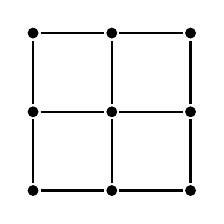
\begin{tikzpicture}[scale=1]
        \begin{scope}
        %\draw[help lines] (-5,-5) grid (5,5);
            \GraphInit[unit=3,vstyle=Normal]
            \SetVertexNormal[Shape=circle, FillColor=black, MinSize=2pt]
            \tikzset{VertexStyle/.append style = {inner sep = \inners, outer sep = \outers}}
            \SetVertexNoLabel
            \Vertex[x=-1,y=-1]{x-1-1}
            \Vertex[x=-1,y=0]{x-10}
            \Vertex[x=-1,y=1]{x-11}
            \Vertex[x=0,y=-1]{x0-1}
            \Vertex[x=0,y=0]{x00}
            \Vertex[x=0,y=1]{x01}
            \Vertex[x=1,y=-1]{x1-1}
            \Vertex[x=1,y=0]{x10}
            \Vertex[x=1,y=1]{x11}

            
            \Edge(x-1-1)(x-10)
            \Edge(x-1-1)(x0-1)
            \Edge(x0-1)(x00)
            \Edge(x0-1)(x1-1)
            
            \Edge(x-10)(x-11)
            \Edge(x-10)(x00)
            \Edge(x00)(x01)
            \Edge(x00)(x10)
            
            \Edge(x-11)(x01)
            \Edge(x01)(x11)
            
            \Edge(x10)(x11)
            \Edge(x10)(x1-1)
        \end{scope}
    \end{tikzpicture}
    \hfill
    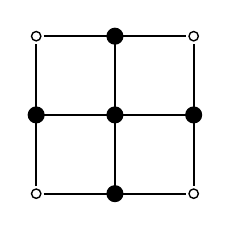
\begin{tikzpicture}[scale=1]
        \begin{scope}
            %\draw[help lines] (-5,-5) grid (5,5);
            \GraphInit[unit=3,vstyle=Normal]
            \SetVertexNormal[Shape=circle, FillColor=white, MinSize=1pt]
            \tikzset{VertexStyle/.append style = {inner sep = \inners, outer sep = \outers}}
            \SetVertexNoLabel
            \Vertex[x=-1,y=-1]{x-1-1}
            \Vertex[x=-1,y=1]{x-11}
            \Vertex[x=1,y=-1]{x1-1}
            \Vertex[x=1,y=1]{x11}
            
            \SetVertexNormal[Shape=circle, FillColor=black, MinSize=1pt]
            \SetVertexNoLabel
            \Vertex[x=0,y=-1]{x0-1}
            \Vertex[x=-1,y=0]{x-10}
            \Vertex[x=1,y=0]{x10}
            \Vertex[x=0,y=0]{x00}
            \Vertex[x=0,y=1]{x01}

            
            \Edge(x-1-1)(x-10)
            \Edge(x-1-1)(x0-1)
            \Edge(x0-1)(x00)
            \Edge(x0-1)(x1-1)
            
            \Edge(x-10)(x-11)
          \Edge(x-10)(x00)
            \Edge(x00)(x01)
            \Edge(x00)(x10)
            
          \Edge(x-11)(x01)
            \Edge(x01)(x11)
            
            \Edge(x10)(x11)
            \Edge(x10)(x1-1)
        \end{scope}
    \end{tikzpicture}
    \hfill
    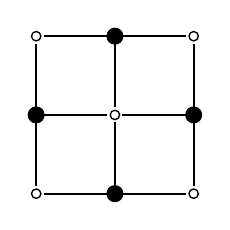
\begin{tikzpicture}[scale=1]
        \begin{scope}
            %\draw[help lines] (-5,-5) grid (5,5);
            \GraphInit[unit=3,vstyle=Normal]
            \SetVertexNormal[Shape=circle, FillColor=white, MinSize=1pt]
            \tikzset{VertexStyle/.append style = {inner sep = \inners, outer sep = \outers}}
            \SetVertexNoLabel
            \Vertex[x=-1,y=-1]{x-1-1}
            \Vertex[x=-1,y=1]{x-11}
            \Vertex[x=1,y=-1]{x1-1}
            \Vertex[x=1,y=1]{x11}
            \Vertex[x=0,y=0]{x00}
            
            \SetVertexNormal[Shape=circle, FillColor=black, MinSize=1pt]
            \SetVertexNoLabel
            \Vertex[x=0,y=-1]{x0-1}
            \Vertex[x=-1,y=0]{x-10}
            \Vertex[x=1,y=0]{x10}
            \Vertex[x=0,y=1]{x01}

            
            \Edge(x-1-1)(x-10)
            \Edge(x-1-1)(x0-1)
            \Edge(x0-1)(x00)
            \Edge(x0-1)(x1-1)
            
            \Edge(x-10)(x-11)
            \Edge(x-10)(x00)
            \Edge(x00)(x01)
            \Edge(x00)(x10)
            
            \Edge(x-11)(x01)
            \Edge(x01)(x11)
            
            \Edge(x10)(x11)
            \Edge(x10)(x1-1)
        \end{scope}
    \end{tikzpicture}

    \caption{From left to right: a graph, one of its maximal bicliques, and a transversal.}
    \label{fig:transversals}
\end{figure}

Drawing inspiration from~\cite{clique_color_algorithm}, we first show the relationships between hypergraph structures and colorings, and use these to build an $\bigOs{2^n}$-time algorithm for \pname{Biclique Coloring} by stating it as an exact cover instance.
Naturally, the covering family must be carefully chosen such that any solution to the covering problem produces a valid coloring.
We first formalize the observation that, given a color~$i$, every maximal biclique of~$G$ must have one color other than~$i$.
%Our first task is to establish a family of sets that can be safely used to cover~$V(G)$,

\begin{lemma}
    \label{lem:transversal_colorings}
    A $k$-partition $\varphi = \{\varphi_1, \dots, \varphi_k\}$ is a $k$-biclique-coloring of $G$ if and only if for every $i$, $\overline{\varphi_i} \in \trans{B}(G)$.
\end{lemma}

%\begin{tproof}
\begin{proof}
    Suppose that there exists some $\varphi_i$ such that $\overline{\varphi_i} \notin \trans{B}(G)$.
    This implies that there exists some $B \in \biq(G)$ such that $B \cap \overline{\varphi_i} = \emptyset$ and that $B \subseteq \varphi_i$; that is, $|\varphi(B)| = 1$, which is a contradiction, since $\varphi$ is a $k$-biclique-coloring.
    
    For the converse, let $\varphi$ be a $k$-partition of $G$ with $\overline{\varphi_i} \in \trans{B}(G)$, but suppose that $\varphi_k$ is not a $k$-biclique-coloring.
    That is, there exists some maximal biclique $B \in \biq(G)$ such that $B \subseteq \varphi_i$ for some $i$.
    This implies that $B \cap \overline{\varphi_i} = \emptyset$, and, therefore, $\overline{\varphi_i} \notin \trans{B}(G)$, which contradicts the hypothesis.
\end{proof}
%\end{tproof}

Simply testing for each $X \in 2^{V(G)}$ if $X \in \transs{B}(G)$ is a costly task.
A naive algorithm would check, for each $B \in \biq(G)$, if $\overline{X} \cap B \neq \emptyset$.
With $|\biq(G)| \in \bigO{n3^{\frac{n}{3}}}$ (see~\cite{gaspers} for the proof), such algorithm would take $\bigO{n2^n3^{\frac{n}{3}}}$-time.
The next Lemma, along with Lemma~\ref{lem:down_closure}, considerably reduces the complexity of enumerating $\trans{B}(G)$.
We will enumerate $\oblq{B}(G)$ by generating its maximal elements and then use the fact that $\oblq{B}(G)$ is closed under the subset operation.

\begin{lemma}
    \label{lem:complementary_obliques}
    The maximal obliques of $\Hyper{B}(G)$ are exactly the complements of the maximal bicliques of $G$.
\end{lemma}

%\begin{tproof}
\begin{proof}
    Let $X \in \oblq{B}$ be a maximal oblique. By definition, there exists some~$B \in \biq(G)$ such that~$X \cap B = \emptyset$, which implies that $X \subseteq \overline{B}$.
    Note that, if $X \subset \overline{B}$, there is some $v \in \overline{B} \setminus X$, which implies that $(X \cup \{v\}) \cap B = \emptyset$ and that $X$ is not a maximal oblique.
    Let $B \in \biq(G)$. By definition, $\overline{B} \in \oblq{B}$ and must be maximal because $\{B, \overline{B}\}$ is a partition of $V(G)$.
\end{proof}
%\end{tproof}

\begin{corollary}
    \label{col:is_maximal_oblique}
    Given a graph $G = (V, E)$ and a subset $X \subseteq V(G)$, there exists an $O(n(n - |X|))$-time algorithm to determine if $X$ is a maximal oblique.
\end{corollary}

\begin{theorem}
    \label{thm:exact_biclique}
    There is an $\bigOs{2^n}$-time algorithm for \pname{Biclique Coloring}.
\end{theorem}

%\begin{tproof}
\begin{proof}
    Our goal is to make use of Theorem~\ref{thm:inc_exc} to solve an instance of \pname{Exact Cover}, with $A = V(G)$, $\mathcal{F} = \transs{B}(G)$ and $k$ the partition size.
    Lemma~\ref{lem:transversal_colorings} guarantees that there is an answer to our instance of \pname{Biclique Coloring} if and only if there is an answer to the corresponding \pname{Exact Cover} one.
    To compute~$\transs{B}(G)$, for each $X \in 2^{V(G)}$, we use Lemma~\ref{lem:complementary_obliques} and Corollary~\ref{col:is_maximal_oblique} to say whether or not $X$ is a maximal oblique of $\Hyper{B}(G)$.
    Next, we compute $\oblq{B}(G)$ from its maximal elements using Lemma~\ref{lem:down_closure}, and use the fact that $\trans{B}(G) = 2^{V(G)} \setminus \oblq{B}(G)$ and complement each transversal to obtain $\transs{B}(G)$.
    Clearly, this procedure takes $\bigOs{2^n}$-time to construct $\transs{B}(G)$ and an additional $\bigOs{2^n}$-time by Theorem~\ref{thm:inc_exc}.
\end{proof}
%\end{tproof}

\subsection{Algorithms parameterized by neighborhood diversity}

\begin{definition}[Neighborhood diversity]
    A graph $G = (V,E)$ has neighborhood diversity $\nd(G) = d$ if it can be $d$-partitioned in $\{D_1, \dots, D_d\}$, with each $D_i$ being a type class of $G$.
\end{definition}

As previously discussed, a type is a maximal set of vertices that are either true or false twins to each other.
If $D_i$ is composed of true twins, we say that it is a \tdef{true twin class} $T_i$ and, clearly, $G[D_i]$ is clique.
Similarly, if $D_i$ is composed of false twins, it is a \tdef{false twin class} $F_i$ and $G[D_i]$ is an independent set.
When $|D_i| = 1$, we treat the class differently depending on the problem.

\subsubsection{Biclique coloring}

For \textsc{biclique coloring}, if there is some $D_i$ with a single vertex, we shall treat it as a true twin class.

\begin{observation}
    \label{obs:biclique_true_twins}
    Given $G$ and a true twin class $T_i$ of $G$, any $k$-biclique-coloring $\varphi$ of $G$ has $|\varphi(T_i)| = |T_i|$.
\end{observation}

\begin{lemma}
    \label{lem:biclique_false_twins}
    Given $G$ and a false twin class $F \subset V(G)$, any  $k$-biclique-coloring $\varphi'$ of $G$ can be changed into a $k$-biclique-coloring $\varphi$ of $G$ such that $|\varphi(F)| \leq 2$.
\end{lemma}

\begin{tproof}
    If $|\varphi'(F)| \leq 2$, $\varphi = \varphi'$.
    Otherwise, there exists $f_1, f_2, f_3 \in F$ with three different colors. 
    Since every maximal biclique $B$ of $G$ with at least one element of $F$ has that $F \subset B$ and thus $|\varphi'(B)| \geq 3$.
    By making $\varphi(f_1) = \varphi'(f_1)$ and $\varphi(f_3) = \varphi(f_2) = \varphi'(f_2)$, we obtain $|\varphi(B)| \geq |\varphi(F)| \geq 2$.
    Repeating this process until $|\varphi(F)| = 2$ does not make any biclique monochromatic and completes the proof.
\end{tproof}

The central idea of our parameterized algorithm is to build an induced subgraph $H$ of $G$ and, afterward, use the results established here and in Section~\ref{sec:biclique_exact} to show that the solution to a particular instance of \textsc{set multicover} derived from $H$ can be transformed in a solution to \textsc{biclique coloring} of $G$.


\begin{definition}[B-Projection and B-Lifting]
    Let $T_i$ and $F_j$ be as previously discussed.
    We define the following projection rules:
    $\forall t_i^q \in T_i,\ \Proj{B}(t_i^q) = \{t'_i\}$;
    for $f_j^1\in F_j,\ \Proj{B}(f_j^1) = \{f'{_j^1}\}$;
    $\forall f_j^r \in F_j \setminus \{f_j^1\}$, $\Proj{B}(f_j^r) = \{f'{_j^2}\}$
    and $\Proj{B}(X) = \bigcup_{u \in X} \Proj{B}(u)$.
    
    Lifting rules are defined as $\Lift{B}(t'_i) = \{t_i\}$; $\Lift{B}(f'{_j^1}) = \{f_j^1\}$; $\Lift{B}(f'{_j^2}) = F_j \setminus \{f_j^1\}$ and $\Lift{B}(Y) = \bigcup_{u \in Y} \Lift{B}(u)$. Note that $\Proj{B}(\Lift{B}(X)) = X$, for any $X$.
\end{definition}


\begin{definition}[B-Projected Graph]
    The B-projected graph $H$ of $G$ is defined as $V(H) = \Proj{B}(V(G))$ and $v'_iv'_j \in E(H)$ if and only if there exist $v_i \in \Lift{B}(v'_i)$ and $v_j \in \Lift{B}(v'_j)$ such that $v_iv_j \in E(G)$. $H$ is an induced subgraph of $G$.
\end{definition}

\begin{figure}[!htb]
    \centering
        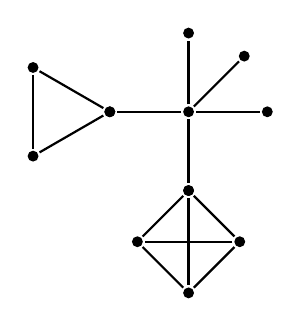
\begin{tikzpicture}[scale=1]
            \GraphInit[unit=3,vstyle=Normal]
            \SetVertexNormal[Shape=circle, FillColor=black, MinSize=2pt]
            \tikzset{VertexStyle/.append style = {inner sep = \inners, outer sep = \outers}}
            \SetVertexNoLabel
            \Vertex[x=0,y=0]{a}
            \Vertex[x=-1,y=0]{b}
            \Vertex[x=0,y=-1]{c}
            
            
            
            \Vertex[x=1,y=0]{h}
            \Vertex[x=0,y=1]{i}
            \Vertex[a=45, d=1]{j}
            
            \Edge(a)(b)
            \Edge(a)(c)
            
            \Edge(a)(h)
            \Edge(a)(i)
            \Edge(a)(j)
            \begin{scope}[shift={(-1.65cm, 0cm)}]
                \grComplete[RA=0.65]{3}
            \end{scope}
            \begin{scope}[shift={(0cm, -1.65cm)}]
                \grComplete[RA=0.65]{4}
            \end{scope}
        \end{tikzpicture}
    \hfill
        \begin{tikzpicture}[scale=1]
            \GraphInit[unit=3,vstyle=Normal]
            \SetVertexNormal[Shape=circle, FillColor=black, MinSize=2pt]
            \tikzset{VertexStyle/.append style = {inner sep = \inners, outer sep = \outers}}
            \SetVertexNoLabel
            \Vertex[x=0,y=0]{a}
            \Vertex[x=-1,y=0]{b}
            \Vertex[x=0,y=-1]{c}
            \Vertex[x=0,y=-1.65]{d}
            \Vertex[x=-1.65,y=0]{e}
            
            
            
            \Vertex[x=1,y=0]{h}
            \Vertex[x=0,y=1]{i}
            
            \Edge(a)(b)
            \Edge(a)(c)
            
            \Edge(a)(h)
            \Edge(a)(i)
            \Edge(b)(e)
            \Edge(c)(d)
        \end{tikzpicture}
    \hfill
    
    
    \caption{A graph (left), and its B-projected graph (right).}
    \label{fig:b-projected}
\end{figure}


For the remainder of this section, $G$ will be the input graph to \textsc{biclique coloring} and $H$ the B-Projected graph of $G$.
Our \textsc{set multicover} instance consists of $V(H)$ as the ground set, $\transs{B}(H)$ as the covering family, the size $k$ of the cover the same as the coloring of $G$ and $c(t_i') = |T_i|$ for every true twin class $T_i$ and $c(f'{_j^1}) = c(f'{_j^2}) = 1$ for each false twin class $F_j$.

The next observation follows directly from the fact that $\transs{B}(H)$ is closed under the subset operation, while the subsequent results allow us to move freely between $\transs{B}(G)$ and $\transs{B}(H)$.

\begin{observation}
    \label{obs:fatless_multicover}
    If there is a minimum $k$-multicover $\psi$ of $V(H)$ by $\transs{B}(H)$, then there exists a minimum $k$-multicover $\psi' = \{\psi_1, \dots, \psi_k\}$ such that $\left|\left\{j \mid u \in \psi_j\right\}\right| = c(u)$ for every $u \in V(H)$.
\end{observation}

\begin{lemma}
    \label{lem:lift_proj_biclique}
    If $B' \in \biq(H)$ then $B = \Lift{B}(B') \in \biq(G)$. Conversely, if $B \in \biq(G)$ and $B$ is not contained in any true twin class, then $B' = \Proj{B}(B) \in \biq(H)$.
\end{lemma}

\begin{tproof}
    ($\Rightarrow$) Note that $B$ is a biclique by the definition of $\Lift{B}$ and the fact that $B'$ is a biclique. By the contrapositive, suppose that $B \notin \biq(G)$ and that $u \in V(G)$ is such that $B \cup \{u\}$ is a (not necessarily maximal) biclique of $G$. Note that either:
    (i) if $u \in F_j$ then $F_j \nsubseteq B$ and $\Proj{B}(u) \notin B'$, because $u \notin \Lift{B}(f'{_j^1})$ or $u \notin \Lift{B}(f'{_j^2})$;
    or (ii) if $u \in T_i$ then $T_i \cap B = \emptyset$, which implies that $\Proj{B}(u) \notin B'$.
    %Since $H$ is an induced subgraph of $G$, no new bicliques can be created in $H$ that were not present in $G$.
    Since $B \cup \{u\}$ is a biclique, $\Proj{B}(u)$ is adjacent to only one partition of $B'$.
    The fact that $\Proj{B}(u) \notin B'$ implies that $\Proj{B}(B \cup \{u\}) = \Proj{B}(B) \cup \Proj{B}(u) = B' \cup \Proj{B}(u)$ is a biclique of $H$ and $B'$ is not maximal.
    
    ($\Leftarrow$) By the definition of $\Proj{B}$, $B' = (X, Y)$ must be a biclique of $H$. By the contrapositive, there is $u' \in V(H)$ such that $B' \cup \{u'\}$ is a (not necessarily maximal) biclique of $H$, and let $u \in \Lift{B}(u')$. By the definition of $\Lift{B}$, it follows that $u$ can only be adjacent to one of partition of $B$, say $\Lift{B}(X)$. Therefore, $u' \in Y$ and, for each $v \in \Lift{B}(Y)$, $uv \notin E(G)$, otherwise there would be $v' \in \Proj{B}(v)$ with $u'v' \in E(H)$. Therefore, $B \cup \{u\}$ is a biclique of $G$ and $B$ is not maximal.
\end{tproof}


\begin{theorem}
    \label{thm:lifted_transversal}
    $X \subseteq V(H)$ is in $\transs{B}(H)$ if and only if $\Lift{B}(X) \in \transs{B}(G)$.
\end{theorem}

\begin{tproof}
    ($\Rightarrow$) Recall that $X \in \transs{B}(H)$ if and only if no maximal biclique of $H$ is contained in $X$.
    It is clear that, for every $B' \in \biq(H)$, $B' \nsubseteq X$ implies that $\Lift{B}(B') \nsubseteq \Lift{B}(X)$, since no two vertices of $H$ are lifted to the same vertex of $G$, and $\Lift{B}(B') \in \biq(G)$ due to Lemma~\ref{lem:lift_proj_biclique}.
    Moreover, no biclique of $G$ entirely contained in a true twin class can be a subset of $\Lift{B}(X)$. As such, $\Lift{B}(X)$ contains a maximal biclique $B$ only if $\Proj{B}(B) \subseteq X$ and $\Proj{B}(B) \notin \biq(H)$, which is impossible due to Lemma~\ref{lem:lift_proj_biclique} and the assumption that $B$ is maximal.
    
    ($\Leftarrow$) Taking the contrapositive, $X \notin \transs{B}(H)$ implies that there is some maximal biclique $B'$ of $H$ such that $B' \subseteq X$. This implies that $\Lift{B}(B') \subseteq \Lift{B}(X)$, and, since $\Lift{B}(B')$ is a maximal biclique of $G$ due to Lemma~\ref{lem:lift_proj_biclique}, it holds that $\Lift{B}(X)$ is not a complement of transversal of $G$.
\end{tproof}


\begin{theorem}
    \label{thm:lifted_multicover}
    $\psi$ is a $k$-multicover of $H$ if and only if $G$ is $k$-biclique-colorable.
\end{theorem}

\begin{tproof}
    Recall that a $k$-partition is a $k$-biclique-coloring if and only if all elements of the partition belong to $\transs{B}(G)$. By the construction of our set multicover instance, we have that, for each $\psi_i$, $\psi_i \in \transs{B}(H)$. By making $\varphi = \left\{\Lift{B}(\psi_1), \dots, \Lift{B}(\psi_k)\right\}$, and recalling Observation~\ref{obs:fatless_multicover}, we have that each vertex $u \in V(H)$ is covered exactly $c(u)$ times; moreover, since true twins appear multiple times and types are equivalence relations, we can attribute to each $t_i^q$ any of the $|T_i|$ colors available, as long as no two receive the same color.
    Therefore, $\varphi$, after properly allocating the true twin classes, is a $k$-partition of $V(G)$.
    Due to Theorem~\ref{thm:lifted_transversal}, every $\Lift{B}(\psi_i)$ is a complement of transversal and therefore $\varphi$ is a valid $k$-biclique-coloring of $G$.
    
    For the converse, we first make use of Lemma~\ref{lem:biclique_false_twins} to guarantee that every false twin class is in at most two color classes. In particular, if two colors are required we force $f_j^1$ to have the smallest color and $F_j \setminus \{f_j^1\}$ to have the other one.
    Afterwards, for every color class $\varphi_i$, we take $\psi_i = \Proj{B}(\varphi_i)$.
    Note that, each color class has at most one element of each $T_i$. Also, for each $F_j$ and any two distinct color classes $\varphi_l, \varphi_r$, $\Proj{B}(\varphi_l) \cap \Proj{B}(\varphi_r) \cap \Proj{B}(F_j) = \emptyset$, since $f_j^1$ has a different color from $F_j \setminus \{f_j^1\}$.
    These observations guarantee that $\Lift{B}(\psi_i) = \varphi_i$ and, because of Theorem~\ref{thm:lifted_transversal}, $\psi_i \in \transs{B}(H)$.
    Finally, $\psi = \{\psi_1, \dots, \psi_k\}$ will be a valid $k$-multicover of $H$ because every vertex of $V(H)$ will be covered the required amount of times.
\end{tproof}

Note that the size of the largest true twin class is exactly the largest coverage requirement $b$ of our \textsc{set multicover} instance. Moreover, since we need at least $b$ colors to biclique color $G$, it holds that $b \leq k$.

\begin{theorem}
    \label{thm:fpt_biclique}
    There exists an $\bigOs{(k+2)^{2\nd(G)}}$ time algorithm to verify if $G$ is $k$-biclique-colorable.
\end{theorem}

\begin{tproof}
        Start by computing the type partition of $G$ in $\bigO{n^3}$ time and building $H$ in $O(n + m)$.
        Afterwards, solve the corresponding \textsc{set multicover} instance in $\bigOs{(k+2)^{2d}}$ time using Theorem~\ref{thm:set_multicover} and lift the multicover using the construction described in the proof of Theorem~\ref{thm:lifted_multicover} in $\bigO{n}$.
\end{tproof}

\subsubsection{Clique coloring}

For \textsc{clique coloring}, a type class with a single vertex is treated as a false twin class.
Unlike \textsc{biclique coloring}, both true and false twin classes are well behaved, one of the reasons we get a much better algorithm for this problem.


\begin{lemma}
    \label{lem:clique_false_twins}
    Given $G$ and a false twin class $F \subset V(G)$, any  $k$-clique-coloring $\varphi'$ can be changed into a $k$-clique-coloring $\varphi$ such that $|\varphi(F)| = 1$.
\end{lemma}

    \begin{tproof}
    If $|\varphi'(F)| = 1$, we are done.
    Otherwise, there exists $f_1, f_2 \in F$ such that $\varphi'(f_1) \neq \varphi'(f_2)$.
    For every maximal clique $C_1$ where $f_1 \in C_1$, define $C' = C \setminus \{f_1\}$ and note that $C_2 = C' \cup \{f_2\}$ is also a maximal clique.
    Since $\varphi'$ is an  coloring $|\varphi'(C') \cup \{\varphi'(f_1)\}| \geq 2$.
    Therefore, making $\varphi(f_2) = \varphi(f_1) = \varphi'(f_1)$ does not make $|\varphi(C_2)| = 1$. 
    Repeating this until $|\varphi(F)| = 1$ does not make any clique that intercepts $F$ monochromatic and completes the proof.
    \end{tproof}
    
\begin{lemma}
    \label{lem:clique_true_twins}
    Given $G$ and  a true twin class $T \subseteq V(G)$, any  $k$-clique-coloring $\varphi'$ can be changed into a $k$-clique-coloring $\varphi$ such that $|\varphi(T)| \leq 2$.
\end{lemma}

\begin{tproof}
    If $|\varphi'(T)| \leq 2$, we are done.
    Otherwise, there exists $t_1, t_2, t_3 \in T$ with different colors.
    Note that, for every maximal clique $C$ that intercepts $T$, $C \subseteq T$.
    Therefore, $|\varphi'(C)| \geq |\varphi'(T)| \geq 3$.
    By making $\varphi(t_1) = \varphi'(t_1)$ and $\varphi(t_3) = \varphi(t_2) = \varphi'(t_2)$ we have $|\varphi(C)| \geq |\varphi(T)| \geq 2$.
    Repeating this process until $|\varphi(T)| \leq 2$ does not make any clique that intercepts $T$ monochromatic and completes the proof.
\end{tproof}

We use sightly different projection and lifting rules for this problem.
However, they still rely on the fact that a type has a constant bound on the number of colors.

\begin{definition}[C-Projection and C-Lifting]
    Let $T_i$ be any true twin class and $F_j$ be any false twin class.
    We define the following projection rules:
    for $t_i^1 \in T_i,\ \Proj{C}(t_i^1) = \{t'{_i^1}\}$,
    $\forall t_i^q \in T_i \setminus \{t_i^1\}$, $\Proj{C}(t_i^q) = \{t'{_i^2}\}$,
    $\forall f_j^r \in F_j$, $\Proj{C}(f_j^r) = \{f'_j\}$
    and $\Proj{C}(X) = \bigcup_{u \in X} \Proj{C}(u)$.
    
    Lifting rules are defined as $\Lift{C}(t'{_i^1}) = \{t_i^1\}$,
    $\Lift{C}(t'{_i^2}) = T_i \setminus \{t_i^1\}$,
    $\Lift{C}(f'_j) = \{f_j^1\}$ and $\Lift{C}(Y) = \bigcup_{u' \in Y} \Lift{C}(u')$. Note that $\Proj{C}(\Lift{C}(X)) = X$, for any $X$.
\end{definition}

\begin{definition}[C-Projected Graph]
    The C-projected graph $H$ of $G$ is defined as $V(H) = \Proj{C}(V(G))$ and $v'_iv'_j \in E(H)$ if and only if $\Lift{C}(v'_i)$ and $\Lift{C}(v'_j)$ are neighbors in $G$. Moreover, $H$ is an induced subgraph of $G$.
\end{definition}

\begin{figure}[!htb]
    \centering
        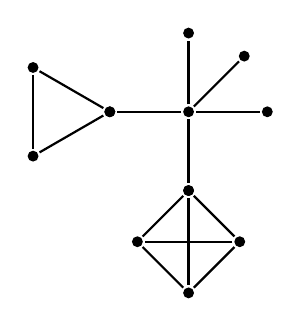
\begin{tikzpicture}[scale=1]
            \GraphInit[unit=3,vstyle=Normal]
            \SetVertexNormal[Shape=circle, FillColor=black, MinSize=2pt]
            \tikzset{VertexStyle/.append style = {inner sep = \inners, outer sep = \outers}}
            \SetVertexNoLabel
            \Vertex[x=0,y=0]{a}
            \Vertex[x=-1,y=0]{b}
            \Vertex[x=0,y=-1]{c}
            
            
            
            \Vertex[x=1,y=0]{h}
            \Vertex[x=0,y=1]{i}
            \Vertex[a=45, d=1]{j}
            
            \Edge(a)(b)
            \Edge(a)(c)
            
            \Edge(a)(h)
            \Edge(a)(i)
            \Edge(a)(j)
            \begin{scope}[shift={(-1.65cm, 0cm)}]
                \grComplete[RA=0.65]{3}
            \end{scope}
            \begin{scope}[shift={(0cm, -1.65cm)}]
                \grComplete[RA=0.65]{4}
            \end{scope}
        \end{tikzpicture}
    \hfill
        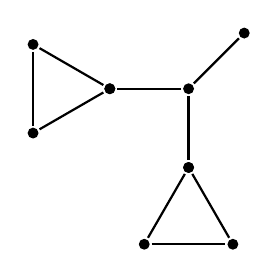
\begin{tikzpicture}[scale=1]
            \GraphInit[unit=3,vstyle=Normal]
            \SetVertexNormal[Shape=circle, FillColor=black, MinSize=2pt]
            \tikzset{VertexStyle/.append style = {inner sep = \inners, outer sep = \outers}}
            \SetVertexNoLabel
            \Vertex[x=0,y=0]{a}
            \Vertex[x=-1,y=0]{b}
            \Vertex[x=0,y=-1]{c}
            
            
            
            \Vertex[a=45, d=1]{j}
            
            \Edge(a)(b)
            \Edge(a)(c)
            
            \Edge(a)(j)
            \begin{scope}[shift={(-1.65cm, 0cm)}]
                \grComplete[RA=0.65]{3}
            \end{scope}
            \begin{scope}[rotate=90,shift={(-1.65cm, 0cm)}]
                \grComplete[RA=0.65]{3}
            \end{scope}
        \end{tikzpicture}
    \hfill
    
    
    \caption{A graph (left), and its C-projected graph (right).}
    \label{fig:c-projected}
\end{figure}


For the remainder of this section, $G$ will be the input graph to \textsc{clique coloring} and $H$ the C-Projected graph of $G$.


\begin{lemma}
    \label{lem:lift_proj_clique}
    If $C' \in \clq(H)$ then $\Lift{C}(C') \in \clq(G)$. Conversely, if $C \in \clq(G)$ then $\Proj{C}(C) \in \clq(H)$.
\end{lemma}

\begin{tproof}
    ($\Rightarrow$) Note that $C = \Lift{C}(C')$ is a clique due to the definition of $\Lift{C}$ and the fact that $C'$ is a clique.
    By the contrapositive, suppose that $C$ is not a maximal clique.
    In this case, there is some vertex $u \in V(G)$ such that $C \cup \{u\}$ is a (not necessarily maximal) clique of $G$. Note that either:
    (i) if $u \in T_i$, $T_i \nsubseteq C$ and $u \notin \Lift{C}(t'{_i^1})$ or $u \notin \Lift{C}(t'{_i^2})$, thus $\Proj{C}(u) \notin C'$;
    (ii) if $u \in F_j$, $F_j \cap C = \emptyset$ and $\Proj{C}(u) \notin C'$.
    Since no two vertices of $H$ are lifted to the same vertex of $G$ and $\Proj{C}(u) \notin C'$, it follows that  $\Proj{C}(C \cup \{u\}) = \Proj{C}(C) \cup \Proj{C}(u) = C' \cup \Proj{C}(u)$ is a clique by the definition of $\Proj{C}$.
    
    ($\Leftarrow$) Clearly, $C' = \Proj{C}(C)$ is a clique of $H$, due to the definition of $\Proj{C}$.
    Suppose, however, that $C' \notin \clq(H)$, which implies that there is some $u' \in V(H)$ such that $C' \cup \{u'\}$ is a clique of $H$ and let $u \in \Lift{C}(u')$.
    By the definition of $\Lift{C}$, $C \subseteq N(u)$ if and only if $\Proj{C}(C) \subseteq N(u')$, which implies that $C'$ is not maximal only if $C$ is not maximal.
    A contradiction that completes the proof.
\end{tproof}

\begin{theorem}
    \label{thm:projected_clique_coloring}
     $G$ is $k$-clique-colorable if and only if $H$ is $k$-clique-colorable.
\end{theorem}

\begin{tproof}
    Let $\varphi_G$ be a $k$-clique-coloring of $G$ that complies with Lemmas~\ref{lem:clique_false_twins} and~\ref{lem:clique_true_twins}.
    Without loss of generality, for every $T_i$, we color $t_i^1$ with one color and $T_i \setminus \{t_i^1\}$ with the other, if it exists, otherwise color every vertex of $T_i$ with the same color.
    We define the $k$-clique-coloring of $H$ as $\varphi_H(u') = \varphi_G(u \in \Lift{C}(u'))$, for every $u' \in V(H)$.
    Suppose now that there exists some $C' \in \clq(H)$ such that $|\varphi_H(C')| = 1$.
    By Lemma~\ref{lem:lift_proj_clique}, $\Lift{C}(C')$ is a maximal clique of $G$ and, since $|\varphi_G\left(\Lift{C}(C')\right)| = 1$, it holds that $\Lift{C}(C')$ is a monochromatic maximal clique of $G$ and $\varphi_G$ is not a valid $k$-clique-coloring, which contradicts the hypothesis.
        
    Now, let $\varphi_H$ be a $k$-clique-coloring of $H$, and define $\varphi_G(u) = \varphi_H(u' \in \Proj{C}(u))$.
    By assuming that there exists some $C \in \clq(G)$ such that $\left|\varphi_G(C)\right| = 1$ and using Lemma~\ref{lem:lift_proj_clique}, it is clear that $\left|\varphi_H(\Proj{C}(C))\right| = 1$ which is impossible, since $\varphi_H$ is a valid $k$-clique-coloring of $H$.
\end{tproof}

\begin{theorem}
    \label{thm:fpt_clique}
    There exists an $\bigOs{2^{2\nd(G)}}$ time algorithm for \textsc{clique coloring}
\end{theorem}

\begin{tproof}
    Start by computing the optimal type partition of $G$ in $\bigO{n^3}$ time and building $H$ in $\bigO{n + m}$.
    Afterwards, color $H$ in $\bigOs{2^{2d}}$ time using Theorem~\ref{thm:clique_color_algorithm} and lift the coloring using the construction described in the proof of Theorem~\ref{thm:projected_clique_coloring} in $\bigO{n}$.
\end{tproof}

%\chapter{Clique and Biclique Coloring}
\label{ch:cb_coloring}

Both \textsc{clique coloring} and \textsc{biclique coloring} are relaxations of the classical \textsc{vertex coloring} problem, in the sense that monochromatic edges are allowed.
However, this freedom comes at the cost of validating a solution, which becomes a $\coNP\text{-}\Complete$ task in both cases.
One may think of \textsc{vertex coloring} as the task of covering a graph's vertices using a given number of independent sets.
That is, there cannot be a color class with an edge inside it.
For \textsc{clique coloring} and \textsc{biclique coloring}, the idea is quite similar.
We want to forbid not edges, but maximal clique or bicliques, respectively, inside our color classes.
All of the following results establish families of sets that may safely be used to cover the given graph and describe how to compute them.

Much of the discussion will deal with the clique and biclique hypergraphs $\Hyper{C}(G)$ and $\Hyper{B}(G)$.
As such, we define by $\trans{C}(G)$ ($\trans{B}(G)$) the \tdef{family of all transversals} of the clique (biclique) hypergraph of $G$ and by $\transs{C}(G)$ ($\transs{B}(G)$) the \tdef{family of complements of transversals}.
Also, denote by $\oblq{C}(G)$ ($\oblq{B}(G)$) the \tdef{family of all obliques} of the clique (biclique) hypergraph of $G$.
Finally, $\clq(G)$ ($\biq(G)$) is the family of \tdef{maximal cliques} (bicliques) of $G$.

In this chapter, we present algorithms that make heavy use of the algorithm described by~\citep{inclusion_exclusion}, which applies the inclusion-exclusion principle to solve a variety of problems in $2^nn^{\bigO{1}}$ time, including \textsc{vertex coloring}.
We denote complexities of the form $f(n)n^{\bigO{1}}$, where $f(n)$ is an exponential function on $n$, by $\bigOs{f(n)}$.

Our main results are an $\bigOs{2^n}$ algorithm for \textsc{biclique coloring}, an $\FPT$ algorithm for \textsc{clique coloring} parameterized by neighbourhood diversity and an $\FPT$ algorithm for \textsc{biclique coloring} parameterized by the number of colors and neighbourhood diversity.
To achieve them, we will rely on the following problems and results of the literature.

\begin{lemma}[\cite{clique_color_algorithm}]
    \label{lem:down_closure}
    For any family $\mathcal{F}$, its down closure $\mathcal{F}_{\downarrow} = \left\{X \subseteq V \mid \exists Y \in \mathcal{F},\ X \subseteq Y\right\}$ can be enumerated in $O^*(|\mc{F}_{\downarrow}|)$ time.
\end{lemma}

\begin{lemma}[\cite{clique_color_algorithm}]
    \label{lem:clique_transversal_colorings}
    A $k$-partition $\varphi = \{\varphi_1, \dots, \varphi_k\}$ is a $k$-clique-coloring of $G$ if and only if for every $i$, $\overline{\varphi_i} \in \trans{C}(G)$.
\end{lemma}

\problem{exact cover}{A set $A = \{a_1, \dots, a_n\}$, a covering family $\mathcal{F} \subseteq 2^A$ and an integer $k$.}{Is it possible to $k$-partition  $A$ into $\varphi$ such that $\varphi \subseteq \mathcal{F}$?}

\begin{theorem}[\cite{inclusion_exclusion}]
    \label{thm:inc_exc}
    There is a $\bigOs{2^n}$ time algorithm to solve \textsc{exact cover}.
\end{theorem}

\begin{theorem}[\cite{clique_color_algorithm}]
    \label{thm:clique_color_algorithm}
    There is an $\bigOs{2^n}$ time algorithm for \textsc{clique coloring}.
\end{theorem}


\problem{set multicover}{A set $A = \{a_1, \dots, a_n\}$, a covering family $\mathcal{F} \subseteq 2^A$, an integer $k$ and a coverage demand $c: A \mapsto \mathbb{N}$.}{Is it possible to $k$-cover $A$ with $\varphi \subseteq \mathcal{F}$ and $\forall a_j, |\{i \mid a_j \in \varphi_i\}| \geq c(a_j)$?}

\begin{theorem}[\cite{set_multicover}]
    \label{thm:set_multicover}
    Set multicover can be solved in $O^*((b+2)^n)$, with $b$ the maximum coverage requirement.
\end{theorem}

\section{Exact algorithm for \textsc{biclique coloring}}
\label{sec:biclique_exact}

\begin{figure}[!htb]
    \centering
    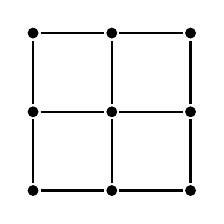
\begin{tikzpicture}[scale=1]
        \begin{scope}
         %\draw[help lines] (-5,-5) grid (5,5);
            \GraphInit[unit=3,vstyle=Normal]
            \SetVertexNormal[Shape=circle, FillColor=black, MinSize=2pt]
            \tikzset{VertexStyle/.append style = {inner sep = \inners, outer sep = \outers}}
            \SetVertexNoLabel
            \Vertex[x=-1,y=-1]{x-1-1}
            \Vertex[x=-1,y=0]{x-10}
            \Vertex[x=-1,y=1]{x-11}
            \Vertex[x=0,y=-1]{x0-1}
            \Vertex[x=0,y=0]{x00}
            \Vertex[x=0,y=1]{x01}
            \Vertex[x=1,y=-1]{x1-1}
            \Vertex[x=1,y=0]{x10}
            \Vertex[x=1,y=1]{x11}

            
            \Edge(x-1-1)(x-10)
            \Edge(x-1-1)(x0-1)
            \Edge(x0-1)(x00)
            \Edge(x0-1)(x1-1)
            
            \Edge(x-10)(x-11)
            \Edge(x-10)(x00)
            \Edge(x00)(x01)
            \Edge(x00)(x10)
            
            \Edge(x-11)(x01)
            \Edge(x01)(x11)
            
            \Edge(x10)(x11)
            \Edge(x10)(x1-1)
        \end{scope}
    \end{tikzpicture}
    \hfill
    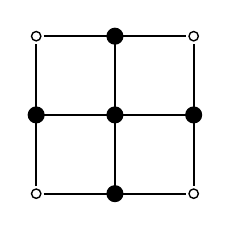
\begin{tikzpicture}[scale=1]
        \begin{scope}
            %\draw[help lines] (-5,-5) grid (5,5);
            \GraphInit[unit=3,vstyle=Normal]
            \SetVertexNormal[Shape=circle, FillColor=white, MinSize=1pt]
            \tikzset{VertexStyle/.append style = {inner sep = \inners, outer sep = \outers}}
            \SetVertexNoLabel
            \Vertex[x=-1,y=-1]{x-1-1}
            \Vertex[x=-1,y=1]{x-11}
            \Vertex[x=1,y=-1]{x1-1}
            \Vertex[x=1,y=1]{x11}
            
            \SetVertexNormal[Shape=circle, FillColor=black, MinSize=1pt]
            \SetVertexNoLabel
            \Vertex[x=0,y=-1]{x0-1}
            \Vertex[x=-1,y=0]{x-10}
            \Vertex[x=1,y=0]{x10}
            \Vertex[x=0,y=0]{x00}
            \Vertex[x=0,y=1]{x01}

            
            \Edge(x-1-1)(x-10)
            \Edge(x-1-1)(x0-1)
            \Edge(x0-1)(x00)
            \Edge(x0-1)(x1-1)
            
            \Edge(x-10)(x-11)
            \Edge(x-10)(x00)
            \Edge(x00)(x01)
            \Edge(x00)(x10)
            
            \Edge(x-11)(x01)
            \Edge(x01)(x11)
            
            \Edge(x10)(x11)
            \Edge(x10)(x1-1)
        \end{scope}
    \end{tikzpicture}
    \hfill
    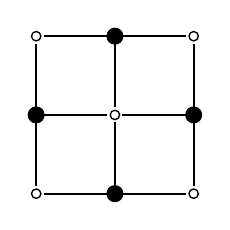
\begin{tikzpicture}[scale=1]
        \begin{scope}
            %\draw[help lines] (-5,-5) grid (5,5);
            \GraphInit[unit=3,vstyle=Normal]
            \SetVertexNormal[Shape=circle, FillColor=white, MinSize=1pt]
            \tikzset{VertexStyle/.append style = {inner sep = \inners, outer sep = \outers}}
            \SetVertexNoLabel
            \Vertex[x=-1,y=-1]{x-1-1}
            \Vertex[x=-1,y=1]{x-11}
            \Vertex[x=1,y=-1]{x1-1}
            \Vertex[x=1,y=1]{x11}
            \Vertex[x=0,y=0]{x00}
            
            \SetVertexNormal[Shape=circle, FillColor=black, MinSize=1pt]
            \SetVertexNoLabel
            \Vertex[x=0,y=-1]{x0-1}
            \Vertex[x=-1,y=0]{x-10}
            \Vertex[x=1,y=0]{x10}
            \Vertex[x=0,y=1]{x01}

            
            \Edge(x-1-1)(x-10)
            \Edge(x-1-1)(x0-1)
            \Edge(x0-1)(x00)
            \Edge(x0-1)(x1-1)
            
            \Edge(x-10)(x-11)
            \Edge(x-10)(x00)
            \Edge(x00)(x01)
            \Edge(x00)(x10)
            
            \Edge(x-11)(x01)
            \Edge(x01)(x11)
            
            \Edge(x10)(x11)
            \Edge(x10)(x1-1)
        \end{scope}
    \end{tikzpicture}
    \hfill
    
    
    \caption{A graph (left), one of its maximal bicliques in black (center), and a transversal in black (right).}
    \label{fig:transversals}
\end{figure}


Our first task is to establish a family of sets that can be safely used to cover $V(G)$, which we accomplish as follows.


\begin{lemma}
    \label{lem:transversal_colorings}
    A $k$-partition $\varphi = \{\varphi_1, \dots, \varphi_k\}$ is a $k$-biclique-coloring of $G$ if and only if for every $i$, $\overline{\varphi_i} \in \trans{B}(G)$.
\end{lemma}

\begin{tproof}
$(\Rightarrow)$ Suppose that there exists some $\varphi_i$ such that $\overline{\varphi_i} \notin \trans{B}(G)$.
This implies that there exists some $B \in \biq(G)$ such that $B \cap \overline{\varphi_i} = \emptyset$ and that $B \subseteq \varphi_i$; that is, $|\varphi(B)| = 1$, which is a contradiction, since $\varphi$ is a $k$-biclique-coloring.

$(\Leftarrow)$ Let $\varphi$ be a $k$-partition of $G$ with $\overline{\varphi_i} \in \trans{B}(G)$, but suppose that $\varphi_k$ is not a $k$-biclique-coloring.
That is, there exists some maximal biclique $B \in \biq(G)$ such that $B \subseteq \varphi_i$ for some $i$.
This implies that $B \cap \overline{\varphi_i} = \emptyset$, and, therefore, $\overline{\varphi_i} \notin \trans{B}(G)$, which contradicts the hypothesis.
\end{tproof}

Simply testing for each $X \in 2^{V(G)}$ if $X \in \transs{B}(G)$ is a costly task.
A naive algorithm would check, for each $B \in \biq(G)$, if $\overline{X} \cap B \neq \emptyset$.
With $|\biq(G)| \in \bigO{n3^{\frac{n}{3}}}$ (see~\citep{gaspers} for the proof), such algorithm would take $\bigO{n2^n3^{\frac{n}{3}}}$ time.

The next Lemma, along with Lemma~\ref{lem:down_closure}, considerably reduce the complexity of enumerating $\trans{B}(G)$.
Effectively, we will enumerate $\oblq{B}(G)$ by first generating its maximal elements and then use the fact that $\oblq{B}(G)$ is closed under the subset operation, which takes $\bigOs{2^n}$ time.

\begin{lemma}
    \label{lem:complementary_obliques}
    The maximal obliques of $\Hyper{B}(G)$ are exactly the complements of the maximal bicliques of $G$.
\end{lemma}

\begin{tproof}
    $(\Rightarrow)$ Let $X \in \oblq{B}$ be a maximal oblique. By definition, there exists some $B \in \biq(G)$ such that $X \cap B = \emptyset$, which implies that $X \subseteq \overline{B}$.
    Note that, if $X \subset \overline{B}$, there is some $v \in \overline{B} \setminus X$, which implies that $(X \cup \{v\}) \cap B = \emptyset$ and that $X$ is not a maximal oblique.
    
    $(\Leftarrow)$ Let $B \in \biq(G)$. By definition, $\overline{B} \in \oblq{B}$ and must be maximal because $\{B, \overline{B}\}$ is a partition of $V(G)$.
\end{tproof}

\begin{corollary}
    \label{col:is_maximal_oblique}
    Given a graph $G = (V, E)$ and a subset $X \subseteq V(G)$, there exists an $O(n(n - |X|))$-time algorithm to determine if $X$ is a maximal oblique.
\end{corollary}

\begin{theorem}
    There is an $\bigOs{2^n}$ time algorithm for \textsc{biclique coloring}.
\end{theorem}

\begin{tproof}
    Our goal is to make use of Theorem~\ref{thm:inc_exc} to solve an instance of \textsc{exact cover}, with $A = V(G)$, $\mathcal{F} = \transs{B}(G)$ and $k$ the partition size.
    Lemma~\ref{lem:transversal_colorings} guarantees that there is an answer to our instance of \textsc{biclique coloring} if and only if there is an answer to the corresponding \textsc{exact cover} instance.
    
    To compute $\transs{B}(G)$, for each $X \in 2^{V(G)}$, we use Lemma~\ref{lem:complementary_obliques} and Corollary~\ref{col:is_maximal_oblique} to say whether or not $X$ is a maximal oblique of $\Hyper{B}(G)$.
    
    Afterwards, we compute $\oblq{B}(G)$ from its maximal elements using Lemma~\ref{lem:down_closure}, and use the fact that $\trans{B}(G) = 2^{V(G)} \setminus \oblq{B}(G)$ and complement each transversal to obtain $\transs{B}(G)$.
    Clearly, this procedure takes $\bigOs{2^n}$ to construct $\transs{B}(G)$ and an additional $\bigOs{2^n}$ to use Theorem~\ref{thm:inc_exc}.
\end{tproof}

\section{Algorithms Parameterized by Neighbourhood Diversity}

\begin{definition}[Neighbourhood Diversity]
    A graph $G = (V,E)$ has neighbourhood diversity $\nd(G) = d$ if it can be $d$-partitioned in $\{D_1, \dots, D_d\}$, with each $D_i$ being a type class of $G$.
\end{definition}

As previously discussed, a type is a maximal set of vertices that are either true or false twins to each other.
If $D_i$ is composed of true twins, we say that it is a \tdef{true twin class} $T_i$ and, clearly, $G[D_i]$ is clique.
Similarly, if $D_i$ is composed of false twins, it is a \tdef{false twin class} $F_i$ and $G[D_i]$ is an independent set.
When $|D_i| = 1$, we treat the class differently depending on the problem.

\subsection{Biclique Coloring}

For \textsc{biclique coloring}, if there is some $D_i$ with a single vertex, we shall treat it as a true twin class.

\begin{observation}
    \label{obs:biclique_true_twins}
    Given $G$ and a true twin class $T_i$ of $G$, any $k$-biclique-coloring $\varphi$ of $G$ has $|\varphi(T_i)| = |T_i|$.
\end{observation}

\begin{lemma}
    \label{lem:biclique_false_twins}
    Given $G$ and a false twin class $F \subset V(G)$, any  $k$-biclique-coloring $\varphi'$ of $G$ can be changed into a $k$-biclique-coloring $\varphi$ of $G$ such that $|\varphi(F)| \leq 2$.
\end{lemma}

\begin{tproof}
    If $|\varphi'(F)| \leq 2$, $\varphi = \varphi'$.
    Otherwise, there exists $f_1, f_2, f_3 \in F$ with three different colors. 
    Since every maximal biclique $B$ of $G$ with at least one element of $F$ has that $F \subset B$ and thus $|\varphi'(B)| \geq 3$.
    By making $\varphi(f_1) = \varphi'(f_1)$ and $\varphi(f_3) = \varphi(f_2) = \varphi'(f_2)$, we obtain $|\varphi(B)| \geq |\varphi(F)| \geq 2$.
    Repeating this process until $|\varphi(F)| = 2$ does not make any biclique monochromatic and completes the proof.
\end{tproof}

The central idea of our parameterized algorithm is to build an induced subgraph $H$ of $G$ and, afterward, use the results established here and in Section~\ref{sec:biclique_exact} to show that the solution to a particular instance of \textsc{set multicover} derived from $H$ can be transformed in a solution to \textsc{biclique coloring} of $G$.


\begin{definition}[B-Projection and B-Lifting]
    Let $T_i$ and $F_j$ be as previously discussed.
    We define the following projection rules:
    $\forall t_i^q \in T_i,\ \Proj{B}(t_i^q) = \{t'_i\}$;
    for $f_j^1\in F_j,\ \Proj{B}(f_j^1) = \{f'{_j^1}\}$;
    $\forall f_j^r \in F_j \setminus \{f_j^1\}$, $\Proj{B}(f_j^r) = \{f'{_j^2}\}$
    and $\Proj{B}(X) = \bigcup_{u \in X} \Proj{B}(u)$.
    
    Lifting rules are defined as $\Lift{B}(t'_i) = \{t_i\}$; $\Lift{B}(f'{_j^1}) = \{f_j^1\}$; $\Lift{B}(f'{_j^2}) = F_j \setminus \{f_j^1\}$ and $\Lift{B}(Y) = \bigcup_{u \in Y} \Lift{B}(u)$. Note that $\Proj{B}(\Lift{B}(X)) = X$, for any $X$.
\end{definition}


\begin{definition}[B-Projected Graph]
    The B-projected graph $H$ of $G$ is defined as $V(H) = \Proj{B}(V(G))$ and $v'_iv'_j \in E(H)$ if and only if there exist $v_i \in \Lift{B}(v'_i)$ and $v_j \in \Lift{B}(v'_j)$ such that $v_iv_j \in E(G)$. $H$ is an induced subgraph of $G$.
\end{definition}

\begin{figure}[!htb]
    \centering
        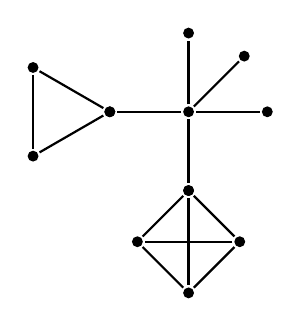
\begin{tikzpicture}[scale=1]
            \GraphInit[unit=3,vstyle=Normal]
            \SetVertexNormal[Shape=circle, FillColor=black, MinSize=2pt]
            \tikzset{VertexStyle/.append style = {inner sep = \inners, outer sep = \outers}}
            \SetVertexNoLabel
            \Vertex[x=0,y=0]{a}
            \Vertex[x=-1,y=0]{b}
            \Vertex[x=0,y=-1]{c}
            
            
            
            \Vertex[x=1,y=0]{h}
            \Vertex[x=0,y=1]{i}
            \Vertex[a=45, d=1]{j}
            
            \Edge(a)(b)
            \Edge(a)(c)
            
            \Edge(a)(h)
            \Edge(a)(i)
            \Edge(a)(j)
            \begin{scope}[shift={(-1.65cm, 0cm)}]
                \grComplete[RA=0.65]{3}
            \end{scope}
            \begin{scope}[shift={(0cm, -1.65cm)}]
                \grComplete[RA=0.65]{4}
            \end{scope}
        \end{tikzpicture}
    \hfill
        \begin{tikzpicture}[scale=1]
            \GraphInit[unit=3,vstyle=Normal]
            \SetVertexNormal[Shape=circle, FillColor=black, MinSize=2pt]
            \tikzset{VertexStyle/.append style = {inner sep = \inners, outer sep = \outers}}
            \SetVertexNoLabel
            \Vertex[x=0,y=0]{a}
            \Vertex[x=-1,y=0]{b}
            \Vertex[x=0,y=-1]{c}
            \Vertex[x=0,y=-1.65]{d}
            \Vertex[x=-1.65,y=0]{e}
            
            
            
            \Vertex[x=1,y=0]{h}
            \Vertex[x=0,y=1]{i}
            
            \Edge(a)(b)
            \Edge(a)(c)
            
            \Edge(a)(h)
            \Edge(a)(i)
            \Edge(b)(e)
            \Edge(c)(d)
        \end{tikzpicture}
    \hfill
    
    
    \caption{A graph (left), and its B-projected graph (right).}
    \label{fig:b-projected}
\end{figure}


For the remainder of this section, $G$ will be the input graph to \textsc{biclique coloring} and $H$ the B-Projected graph of $G$.
Our \textsc{set multicover} instance consists of $V(H)$ as the ground set, $\transs{B}(H)$ as the covering family, the size $k$ of the cover the same as the coloring of $G$ and $c(t_i') = |T_i|$ for every true twin class $T_i$ and $c(f'{_j^1}) = c(f'{_j^2}) = 1$ for each false twin class $F_j$.

The next observation follows directly from the fact that $\transs{B}(H)$ is closed under the subset operation, while the subsequent results allow us to move freely between $\transs{B}(G)$ and $\transs{B}(H)$.

\begin{observation}
    \label{obs:fatless_multicover}
    If there is a minimum $k$-multicover $\psi$ of $V(H)$ by $\transs{B}(H)$, then there exists a minimum $k$-multicover $\psi' = \{\psi_1, \dots, \psi_k\}$ such that $\left|\left\{j \mid u \in \psi_j\right\}\right| = c(u)$ for every $u \in V(H)$.
\end{observation}

\begin{lemma}
    \label{lem:lift_proj_biclique}
    If $B' \in \biq(H)$ then $B = \Lift{B}(B') \in \biq(G)$. Conversely, if $B \in \biq(G)$ and $B$ is not contained in any true twin class, then $B' = \Proj{B}(B) \in \biq(H)$.
\end{lemma}

\begin{tproof}
    ($\Rightarrow$) Note that $B$ is a biclique by the definition of $\Lift{B}$ and the fact that $B'$ is a biclique. By the contrapositive, suppose that $B \notin \biq(G)$ and that $u \in V(G)$ is such that $B \cup \{u\}$ is a (not necessarily maximal) biclique of $G$. Note that either:
    (i) if $u \in F_j$ then $F_j \nsubseteq B$ and $\Proj{B}(u) \notin B'$, because $u \notin \Lift{B}(f'{_j^1})$ or $u \notin \Lift{B}(f'{_j^2})$;
    or (ii) if $u \in T_i$ then $T_i \cap B = \emptyset$, which implies that $\Proj{B}(u) \notin B'$.
    %Since $H$ is an induced subgraph of $G$, no new bicliques can be created in $H$ that were not present in $G$.
    Since $B \cup \{u\}$ is a biclique, $\Proj{B}(u)$ is adjacent to only one partition of $B'$.
    The fact that $\Proj{B}(u) \notin B'$ implies that $\Proj{B}(B \cup \{u\}) = \Proj{B}(B) \cup \Proj{B}(u) = B' \cup \Proj{B}(u)$ is a biclique of $H$ and $B'$ is not maximal.
    
    ($\Leftarrow$) By the definition of $\Proj{B}$, $B' = (X, Y)$ must be a biclique of $H$. By the contrapositive, there is $u' \in V(H)$ such that $B' \cup \{u'\}$ is a (not necessarily maximal) biclique of $H$, and let $u \in \Lift{B}(u')$. By the definition of $\Lift{B}$, it follows that $u$ can only be adjacent to one of partition of $B$, say $\Lift{B}(X)$. Therefore, $u' \in Y$ and, for each $v \in \Lift{B}(Y)$, $uv \notin E(G)$, otherwise there would be $v' \in \Proj{B}(v)$ with $u'v' \in E(H)$. Therefore, $B \cup \{u\}$ is a biclique of $G$ and $B$ is not maximal.
\end{tproof}


\begin{theorem}
    \label{thm:lifted_transversal}
    $X \subseteq V(H)$ is in $\transs{B}(H)$ if and only if $\Lift{B}(X) \in \transs{B}(G)$.
\end{theorem}

\begin{tproof}
    ($\Rightarrow$) Recall that $X \in \transs{B}(H)$ if and only if no maximal biclique of $H$ is contained in $X$.
    It is clear that, for every $B' \in \biq(H)$, $B' \nsubseteq X$ implies that $\Lift{B}(B') \nsubseteq \Lift{B}(X)$, since no two vertices of $H$ are lifted to the same vertex of $G$, and $\Lift{B}(B') \in \biq(G)$ due to Lemma~\ref{lem:lift_proj_biclique}.
    Moreover, no biclique of $G$ entirely contained in a true twin class can be a subset of $\Lift{B}(X)$. As such, $\Lift{B}(X)$ contains a maximal biclique $B$ only if $\Proj{B}(B) \subseteq X$ and $\Proj{B}(B) \notin \biq(H)$, which is impossible due to Lemma~\ref{lem:lift_proj_biclique} and the assumption that $B$ is maximal.
    
    ($\Leftarrow$) Taking the contrapositive, $X \notin \transs{B}(H)$ implies that there is some maximal biclique $B'$ of $H$ such that $B' \subseteq X$. This implies that $\Lift{B}(B') \subseteq \Lift{B}(X)$, and, since $\Lift{B}(B')$ is a maximal biclique of $G$ due to Lemma~\ref{lem:lift_proj_biclique}, it holds that $\Lift{B}(X)$ is not a complement of transversal of $G$.
\end{tproof}


\begin{theorem}
    \label{thm:lifted_multicover}
    $\psi$ is a $k$-multicover of $H$ if and only if $G$ is $k$-biclique-colorable.
\end{theorem}

\begin{tproof}
    Recall that a $k$-partition is a $k$-biclique-coloring if and only if all elements of the partition belong to $\transs{B}(G)$. By the construction of our set multicover instance, we have that, for each $\psi_i$, $\psi_i \in \transs{B}(H)$. By making $\varphi = \left\{\Lift{B}(\psi_1), \dots, \Lift{B}(\psi_k)\right\}$, and recalling Observation~\ref{obs:fatless_multicover}, we have that each vertex $u \in V(H)$ is covered exactly $c(u)$ times; moreover, since true twins appear multiple times and types are equivalence relations, we can attribute to each $t_i^q$ any of the $|T_i|$ colors available, as long as no two receive the same color.
    Therefore, $\varphi$, after properly allocating the true twin classes, is a $k$-partition of $V(G)$.
    Due to Theorem~\ref{thm:lifted_transversal}, every $\Lift{B}(\psi_i)$ is a complement of transversal and therefore $\varphi$ is a valid $k$-biclique-coloring of $G$.
    
    For the converse, we first make use of Lemma~\ref{lem:biclique_false_twins} to guarantee that every false twin class is in at most two color classes. In particular, if two colors are required we force $f_j^1$ to have the smallest color and $F_j \setminus \{f_j^1\}$ to have the other one.
    Afterwards, for every color class $\varphi_i$, we take $\psi_i = \Proj{B}(\varphi_i)$.
    Note that, each color class has at most one element of each $T_i$. Also, for each $F_j$ and any two distinct color classes $\varphi_l, \varphi_r$, $\Proj{B}(\varphi_l) \cap \Proj{B}(\varphi_r) \cap \Proj{B}(F_j) = \emptyset$, since $f_j^1$ has a different color from $F_j \setminus \{f_j^1\}$.
    These observations guarantee that $\Lift{B}(\psi_i) = \varphi_i$ and, because of Theorem~\ref{thm:lifted_transversal}, $\psi_i \in \transs{B}(H)$.
    Finally, $\psi = \{\psi_1, \dots, \psi_k\}$ will be a valid $k$-multicover of $H$ because every vertex of $V(H)$ will be covered the required amount of times.
\end{tproof}

Note that the size of the largest true twin class is exactly the largest coverage requirement $b$ of our \textsc{set multicover} instance. Moreover, since we need at least $b$ colors to biclique color $G$, it holds that $b \leq k$.

\begin{theorem}
    \label{thm:fpt_biclique}
    There exists an $\bigOs{(k+2)^{2\nd(G)}}$ time algorithm to verify if $G$ is $k$-biclique-colorable.
\end{theorem}

\begin{tproof}
        Start by computing the type partition of $G$ in $\bigO{n^3}$ time and building $H$ in $O(n + m)$.
        Afterwards, solve the corresponding \textsc{set multicover} instance in $\bigOs{(k+2)^{2d}}$ time using Theorem~\ref{thm:set_multicover} and lift the multicover using the construction described in the proof of Theorem~\ref{thm:lifted_multicover} in $\bigO{n}$.
\end{tproof}

\subsection{Clique Coloring}

For \textsc{clique coloring}, a type class with a single vertex is treated as a false twin class.
Unlike \textsc{biclique coloring}, both true and false twin classes are well behaved, one of the reasons we get a much better algorithm for this problem.


\begin{lemma}
    \label{lem:clique_false_twins}
    Given $G$ and a false twin class $F \subset V(G)$, any  $k$-clique-coloring $\varphi'$ can be changed into a $k$-clique-coloring $\varphi$ such that $|\varphi(F)| = 1$.
\end{lemma}

    \begin{tproof}
    If $|\varphi'(F)| = 1$, we are done.
    Otherwise, there exists $f_1, f_2 \in F$ such that $\varphi'(f_1) \neq \varphi'(f_2)$.
    For every maximal clique $C_1$ where $f_1 \in C_1$, define $C' = C \setminus \{f_1\}$ and note that $C_2 = C' \cup \{f_2\}$ is also a maximal clique.
    Since $\varphi'$ is an  coloring $|\varphi'(C') \cup \{\varphi'(f_1)\}| \geq 2$.
    Therefore, making $\varphi(f_2) = \varphi(f_1) = \varphi'(f_1)$ does not make $|\varphi(C_2)| = 1$. 
    Repeating this until $|\varphi(F)| = 1$ does not make any clique that intercepts $F$ monochromatic and completes the proof.
    \end{tproof}
    
\begin{lemma}
    \label{lem:clique_true_twins}
    Given $G$ and  a true twin class $T \subseteq V(G)$, any  $k$-clique-coloring $\varphi'$ can be changed into a $k$-clique-coloring $\varphi$ such that $|\varphi(T)| \leq 2$.
\end{lemma}

\begin{tproof}
    If $|\varphi'(T)| \leq 2$, we are done.
    Otherwise, there exists $t_1, t_2, t_3 \in T$ with different colors.
    Note that, for every maximal clique $C$ that intercepts $T$, $C \subseteq T$.
    Therefore, $|\varphi'(C)| \geq |\varphi'(T)| \geq 3$.
    By making $\varphi(t_1) = \varphi'(t_1)$ and $\varphi(t_3) = \varphi(t_2) = \varphi'(t_2)$ we have $|\varphi(C)| \geq |\varphi(T)| \geq 2$.
    Repeating this process until $|\varphi(T)| \leq 2$ does not make any clique that intercepts $T$ monochromatic and completes the proof.
\end{tproof}

We use sightly different projection and lifting rules for this problem.
However, they still rely on the fact that a type has a constant bound on the number of colors.

\begin{definition}[C-Projection and C-Lifting]
    Let $T_i$ be any true twin class and $F_j$ be any false twin class.
    We define the following projection rules:
    for $t_i^1 \in T_i,\ \Proj{C}(t_i^1) = \{t'{_i^1}\}$,
    $\forall t_i^q \in T_i \setminus \{t_i^1\}$, $\Proj{C}(t_i^q) = \{t'{_i^2}\}$,
    $\forall f_j^r \in F_j$, $\Proj{C}(f_j^r) = \{f'_j\}$
    and $\Proj{C}(X) = \bigcup_{u \in X} \Proj{C}(u)$.
    
    Lifting rules are defined as $\Lift{C}(t'{_i^1}) = \{t_i^1\}$,
    $\Lift{C}(t'{_i^2}) = T_i \setminus \{t_i^1\}$,
    $\Lift{C}(f'_j) = \{f_j^1\}$ and $\Lift{C}(Y) = \bigcup_{u' \in Y} \Lift{C}(u')$. Note that $\Proj{C}(\Lift{C}(X)) = X$, for any $X$.
\end{definition}

\begin{definition}[C-Projected Graph]
    The C-projected graph $H$ of $G$ is defined as $V(H) = \Proj{C}(V(G))$ and $v'_iv'_j \in E(H)$ if and only if $\Lift{C}(v'_i)$ and $\Lift{C}(v'_j)$ are neighbours in $G$. Moreover, $H$ is an induced subgraph of $G$.
\end{definition}

\begin{figure}[!htb]
    \centering
        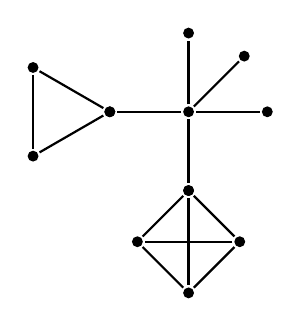
\begin{tikzpicture}[scale=1]
            \GraphInit[unit=3,vstyle=Normal]
            \SetVertexNormal[Shape=circle, FillColor=black, MinSize=2pt]
            \tikzset{VertexStyle/.append style = {inner sep = \inners, outer sep = \outers}}
            \SetVertexNoLabel
            \Vertex[x=0,y=0]{a}
            \Vertex[x=-1,y=0]{b}
            \Vertex[x=0,y=-1]{c}
            
            
            
            \Vertex[x=1,y=0]{h}
            \Vertex[x=0,y=1]{i}
            \Vertex[a=45, d=1]{j}
            
            \Edge(a)(b)
            \Edge(a)(c)
            
            \Edge(a)(h)
            \Edge(a)(i)
            \Edge(a)(j)
            \begin{scope}[shift={(-1.65cm, 0cm)}]
                \grComplete[RA=0.65]{3}
            \end{scope}
            \begin{scope}[shift={(0cm, -1.65cm)}]
                \grComplete[RA=0.65]{4}
            \end{scope}
        \end{tikzpicture}
    \hfill
        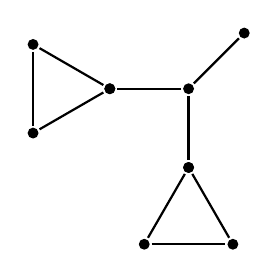
\begin{tikzpicture}[scale=1]
            \GraphInit[unit=3,vstyle=Normal]
            \SetVertexNormal[Shape=circle, FillColor=black, MinSize=2pt]
            \tikzset{VertexStyle/.append style = {inner sep = \inners, outer sep = \outers}}
            \SetVertexNoLabel
            \Vertex[x=0,y=0]{a}
            \Vertex[x=-1,y=0]{b}
            \Vertex[x=0,y=-1]{c}
            
            
            
            \Vertex[a=45, d=1]{j}
            
            \Edge(a)(b)
            \Edge(a)(c)
            
            \Edge(a)(j)
            \begin{scope}[shift={(-1.65cm, 0cm)}]
                \grComplete[RA=0.65]{3}
            \end{scope}
            \begin{scope}[rotate=90,shift={(-1.65cm, 0cm)}]
                \grComplete[RA=0.65]{3}
            \end{scope}
        \end{tikzpicture}
    \hfill
    
    
    \caption{A graph (left), and its C-projected graph (right).}
    \label{fig:c-projected}
\end{figure}


For the remainder of this section, $G$ will be the input graph to \textsc{clique coloring} and $H$ the C-Projected graph of $G$.


\begin{lemma}
    \label{lem:lift_proj_clique}
    If $C' \in \clq(H)$ then $\Lift{C}(C') \in \clq(G)$. Conversely, if $C \in \clq(G)$ then $\Proj{C}(C) \in \clq(H)$.
\end{lemma}

\begin{tproof}
    ($\Rightarrow$) Note that $C = \Lift{C}(C')$ is a clique due to the definition of $\Lift{C}$ and the fact that $C'$ is a clique.
    By the contrapositive, suppose that $C$ is not a maximal clique.
    In this case, there is some vertex $u \in V(G)$ such that $C \cup \{u\}$ is a (not necessarily maximal) clique of $G$. Note that either:
    (i) if $u \in T_i$, $T_i \nsubseteq C$ and $u \notin \Lift{C}(t'{_i^1})$ or $u \notin \Lift{C}(t'{_i^2})$, thus $\Proj{C}(u) \notin C'$;
    (ii) if $u \in F_j$, $F_j \cap C = \emptyset$ and $\Proj{C}(u) \notin C'$.
    Since no two vertices of $H$ are lifted to the same vertex of $G$ and $\Proj{C}(u) \notin C'$, it follows that  $\Proj{C}(C \cup \{u\}) = \Proj{C}(C) \cup \Proj{C}(u) = C' \cup \Proj{C}(u)$ is a clique by the definition of $\Proj{C}$.
    
    ($\Leftarrow$) Clearly, $C' = \Proj{C}(C)$ is a clique of $H$, due to the definition of $\Proj{C}$.
    Suppose, however, that $C' \notin \clq(H)$, which implies that there is some $u' \in V(H)$ such that $C' \cup \{u'\}$ is a clique of $H$ and let $u \in \Lift{C}(u')$.
    By the definition of $\Lift{C}$, $C \subseteq N(u)$ if and only if $\Proj{C}(C) \subseteq N(u')$, which implies that $C'$ is not maximal only if $C$ is not maximal.
    A contradiction that completes the proof.
\end{tproof}

\begin{theorem}
    \label{thm:projected_clique_coloring}
     $G$ is $k$-clique-colorable if and only if $H$ is $k$-clique-colorable.
\end{theorem}

\begin{tproof}
    Let $\varphi_G$ be a $k$-clique-coloring of $G$ that complies with Lemmas~\ref{lem:clique_false_twins} and~\ref{lem:clique_true_twins}.
    Without loss of generality, for every $T_i$, we color $t_i^1$ with one color and $T_i \setminus \{t_i^1\}$ with the other, if it exists, otherwise color every vertex of $T_i$ with the same color.
    We define the $k$-clique-coloring of $H$ as $\varphi_H(u') = \varphi_G(u \in \Lift{C}(u'))$, for every $u' \in V(H)$.
    Suppose now that there exists some $C' \in \clq(H)$ such that $|\varphi_H(C')| = 1$.
    By Lemma~\ref{lem:lift_proj_clique}, $\Lift{C}(C')$ is a maximal clique of $G$ and, since $|\varphi_G\left(\Lift{C}(C')\right)| = 1$, it holds that $\Lift{C}(C')$ is a monochromatic maximal clique of $G$ and $\varphi_G$ is not a valid $k$-clique-coloring, which contradicts the hypothesis.
        
    Now, let $\varphi_H$ be a $k$-clique-coloring of $H$, and define $\varphi_G(u) = \varphi_H(u' \in \Proj{C}(u))$.
    By assuming that there exists some $C \in \clq(G)$ such that $\left|\varphi_G(C)\right| = 1$ and using Lemma~\ref{lem:lift_proj_clique}, it is clear that $\left|\varphi_H(\Proj{C}(C))\right| = 1$ which is impossible, since $\varphi_H$ is a valid $k$-clique-coloring of $H$.
\end{tproof}

\begin{theorem}
    \label{thm:fpt_clique}
    There exists an $\bigOs{2^{2\nd(G)}}$ time algorithm for \textsc{clique coloring}
\end{theorem}

\begin{tproof}
    Start by computing the optimal type partition of $G$ in $\bigO{n^3}$ time and building $H$ in $\bigO{n + m}$.
    Afterwards, color $H$ in $\bigOs{2^{2d}}$ time using Theorem~\ref{thm:clique_color_algorithm} and lift the coloring using the construction described in the proof of Theorem~\ref{thm:projected_clique_coloring} in $\bigO{n}$.
\end{tproof}

%\chapter{Finding Cuts of Bounded Degree}

\section{Definitions and related work}

A \tdef{cut} of a graph $G = (V, E)$ is a bipartition of its vertex set $V(G)$ into two non-empty sets, denoted by $(A,B)$.
The set of all edges with one endpoint in $A$ and the other in $B$ is the \tdef{edge cut}, or the set of \tdef{crossing edges}, of $(A,B)$.
In a slight abuse of notation, we also denote the set of crossing edges by $(A,B)$.
A \tdef{matching cut} is a (possibly empty) edge cut that is a matching, i.e., its edges are pairwise vertex-disjoint.
Equivalently, $(A, B)$ is a matching cut of $G$ if and only if every vertex is incident to at most one crossing edge of $(A, B)$~\citep{matching_cut_graham, chvatal_matching_cut}, that is, it has at most one neighbor across the cut.
The \pname{Matching Cut} problem is, thus, the task of deciding whether a graph admits a matching cut.
Figure~\ref{fig:matching_cut} gives an example of a graph with a matching cut.

\problem{Matching Cut}{A graph $G$.}{Does $G$ have a matching cut?}


\begin{figure}[!htb]
        \centering
        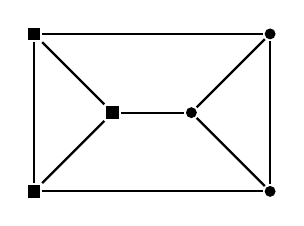
\begin{tikzpicture}[rotate = 0]
                %\draw[help lines] (-5,-5) grid (5,5);
                \GraphInit[unit=3,vstyle=Normal]
                \SetVertexNormal[Shape=circle, FillColor = black, MinSize=3pt]
                \tikzset{VertexStyle/.append style = {inner sep = \inners, outer sep = \outers}}
                \SetVertexNoLabel
                
                \begin{scope}[rotate=90, shift={(0, 2)}]
                    \tikzset{VertexStyle/.append style = {shape = rectangle, inner sep = 2pt}}
                    \grComplete[RA=1]{2}
                \end{scope}
                \begin{scope}[rotate = 90, shift={(0, -1)}]
                    \grComplete[RA=1,prefix=b]{2}
                \end{scope}
                \begin{scope}
                    \tikzset{VertexStyle/.append style = {shape = rectangle, inner sep = 2pt}}
                    \Vertex[x=-1, y=0]{f}
                \end{scope}
                \Vertex[x=0, y=0]{g}
                \Edges(g,b0,a0,f,a1,b1,g,f)
        \end{tikzpicture}
        \caption{Example of a matching cut. Square vertices would be assigned to $A$, circles to $B$.\label{fig:matching_cut}}
    \end{figure}


Motivated by an open question posed by \cite{matching_cut_ipec} during the presentation of their article,  we investigate a natural generalization that arises from this alternative definition.
For a positive integer $d \geq 1$, a \tdef{$d$-cut} is a cut $(A, B)$ such that each vertex has at most $d$ neighbors across the partition, that is, every vertex in $A$ has at most $d$ neighbors in $B$, and vice-versa. Note that a $1$-cut is a matching cut.
As expected, not every graph admits a $d$-cut, and the \pname{$d$-Cut} problem is the problem of, for a fixed integer $d \geq 1$, deciding whether or not an input graph $G$ has a $d$-cut.

\problem{$d$-Cut}{A graph $G$.}{Does $G$ admit a $d$-cut?}

When $d=1$, the problem is known as \pname{Matching Cut}.
Graphs with no matching cut first appeared in Graham's manuscript~\citep{matching_cut_graham} under the name of \textit{indecomposable graphs}, presenting some examples and properties of decomposable and indecomposable graphs, leaving their recognition as an open problem.
In answer to Graham's question, \cite{chvatal_matching_cut} proved that the problem is \NP-hard for graphs of maximum degree at least four and polynomially solvable for graphs of maximum degree at most three; in fact, as shown by \cite{matching_cut_moshi}, every graph of maximum degree three and at least eight vertices has a matching cut.

Chvátal's results spurred a lot of research on the complexity of the problem~\citep{matching_cut_ipec,matching_cut_structural,matching_cut_tcs, matching_cut_diameter, matching_cut_planar, matching_cut_series_parallel, stable_cutset_line_graphs}.
In particular, \cite{matching_cut_planar} showed that \pname{Matching Cut} remains \NP-hard for planar graphs of maximum degree four and for planar graphs of girth five;
\cite{stable_cutset_line_graphs} gave an \NP-hardness reduction for bipartite graphs of maximum degree four;
\cite{matching_cut_diameter} proved that \pname{Matching Cut} is \NP-hard for graphs of diameter at least three, and presented a polynomial-time algorithm for graphs of diameter at most two.
Beyond planar graphs, \cite{matching_cut_planar} also proves that the matching cut property is expressible in monadic second order logic and, by Courcelle's Theorem~\citep{courcelle_theorem}, it follows that \pname{Matching Cut} is $\FPT$ when parameterized by the treewidth of the input graph; he concludes with a proof that the problem admits a polynomial-time algorithm for graphs of bounded cliquewidth.

\cite{matching_cut_tcs} noted that Chv\'atal's original reduction also shows that, unless the Exponential Time Hypothesis fails, there is no algorithm solving \pname{Matching Cut} in time $2^{o(n)}$ on $n$-vertex input graphs.
Also in~\citep{matching_cut_tcs}, the authors provide a first branching algorithm, running in time $\bigOs{2^{n/2}}$, a single-exponential $\FPT$ algorithm when parameterized by the vertex cover number $\tau(G)$, and an algorithm generalizing the polynomial cases of line graphs~\citep{matching_cut_moshi} and claw-free graphs~\citep{matching_cut_planar}.
\cite{matching_cut_tcs} also asked for the existence of a single-exponential algorithm parameterized by treewidth.
In response, \cite{matching_cut_structural} provided a $\bigOs{12^{\tw(G)}}$ algorithm for \pname{Matching Cut} using nice tree decompositions, along with $\FPT$ algorithms for other structural parameters, namely neighborhood diversity, twin-cover, and distance to split graph.

The natural parameter -- the number of edges crossing the cut -- has also been considered.
Indeed, \cite{marx_treewidth_reduction} tackled the \pname{Stable Cutset} problem, to which \pname{Matching Cut} can be easily reduced via the line graph, and through a breakthrough technique showed that this problem is $\FPT$ when parameterized by the maximum size of the stable cutset.
Recently, \cite{matching_cut_ipec} improved on the results of \cite{matching_cut_tcs}, providing an exact exponential algorithm for \pname{Matching Cut} running in  time $\bigOs{1.3803^n}$, as well as $\FPT$ algorithms parameterized by the distance to a cluster graph and the distance to a co-cluster graph, which improve the algorithm parameterized by the vertex cover number, since both parameters are easily seen to be smaller than the vertex cover number.
For the distance to cluster parameter, they also presented a quadratic kernel; while for a combination of treewidth, maximum degree, and number of crossing edges, they showed that no polynomial kernel exists unless $\NP \subseteq \coNP/\poly$.

A problem  closely related to \pname{$d$-Cut} is that of \pname{Internal Partition}, first studied by \cite{internal_partition_thomassen}.
In this problem, we seek a bipartition of the vertices of an input graph such that every vertex has at least as many neighbors in its
own part as in the other part. Such a partition is called an \tdef{internal partition}.
Usually, the problem is posed in a more general form: given functions $a,b: V(G) \rightarrow \mathbb{Z}_+$, we seek a bipartition $(A,B)$ of $V(G)$ such that every $v \in A$ satisfies $\dgr_A(v) \geq a(v)$ and every $u \in B$ satisfies $\dgr_B(u) \geq b(u)$, where $\dgr_A(v)$ denotes the number of neighbors of $v$ in the set $A$. Such a partition is called an \tdef{$(a,b)$-internal partition}.

Originally, Thomassen asked in~\citep{internal_partition_thomassen} whether for any pair of positive integers $s,t$, a graph $G$ with $\delta(G) \geq s + t + 1$ has a vertex bipartition $(A,B)$ with $\delta(G[A]) \geq s$ and $\delta(G[B]) \geq t$.
\cite{internal_partition_stiebitz} answered that, in fact, for any graph $G$ and any pair of functions $a,b: V(G) \rightarrow \mathbb{Z}_+$ satisfying $\dgr(v) \geq a(v) + b(v) + 1$ for every $v \in V(G)$, $G$ has an $(a,b)$-internal partition.
Following Stiebitz's work, \cite{internal_partition_triangle_free} showed that if $G$ is triangle-free, then the pair $a,b$ only needs to satisfy $\dgr(v) \geq a(v) + b(v)$.
More recently, \cite{internal_partition_c4_free} proved that, if $G$ is $\{C_4, K_4, \text{diamond}\}$-free, then $\dgr(v) \geq a(v) + b(v) - 1$ is enough.
Furthermore, they also showed, for any pair $a,b$, a family of graphs such that $\dgr(v) \geq a(v) + b(v) - 2$ for every $v \in V(G)$ that do not admit an $(a,b)$-internal partition.

It is conjectured that, for every positive integer $r$, there exists some constant $n_r$ for which every $r$-regular graph with more than $n_r$ vertices has an internal partition~\citep{DeVos09,internal_partition_regular6} (the conjecture for $r$ even appeared first in~\citep{internal_partition_regular3_4}).
The cases $r \in \{3,4\}$ have been settled by \cite{internal_partition_regular3_4}; the case $r=6$ has been verified by \cite{internal_partition_regular6}.
This latter result implies that every 6-regular graph of sufficiently large size has a 3-cut.
\section{NP-hardness, polynomial cases, and exact exponential algorithm}
\label{sec:np}

In this section we focus on the classical complexity of the \textsc{$d$-Cut} problem, and on exact exponential algorithms. Namely, we provide the \NP-hardness result in Section~\ref{sec:NP-hard}, the polynomial algorithm for graphs of bounded degree in Section~\ref{sec:poly-algo}, and 
a simple exact exponential algorithm in Section~\ref{sec:exact-algo}.

\subsection{NP-hardness for regular graphs}
\label{sec:NP-hard}

Before stating our \NP-hardness result, we need some definitions and observations.

\begin{definition}
    A set of vertices $X \subseteq V(G)$ is said to be \emph{monochromatic} if, for any $d$-cut $(A, B)$ of $G$, $X \subseteq A$ or $X \subseteq B$.
\end{definition}

\begin{observation}
    \label{obs:mono_bipartite}
    For fixed $d \geq 1$, the graph $K_{d+1, 2d+1}$ is monochromatic.
    Moreover, any vertex with $d+1$ neighbors in a monochromatic set is monochromatic.
\end{observation}

\begin{definition}[Spool]
    For $n,d \geq 1$, a \emph{$(d, n)$-spool}  is the graph obtained from $n$  copies of $K_{d+1, 2d+2}$ such that, for every $1 \leq i \leq n$, one vertex of degree $d+1$ of the $i$-th copy is identified with one vertex of degree $d+1$ of the $(i+1 \mod n)$-th copy, so that the two chosen vertices in each copy are distinct. %\ig{we need to say that, within each copy, the two ``identified'' vertices are distinct}.
    The \emph{exterior} vertices of a copy are those of degree $d+1$ that are not used to interface with another copy.
    The \emph{interior} vertices of a copy are those of degree $2d+2$ that do not interface with another copy.
\end{definition}

An illustration of a $(2,3)$-spool is shown in Figure~\ref{fig:spool}.

\begin{figure}[!htb]
    \centering
    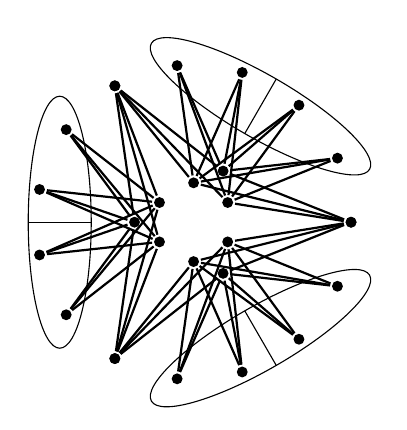
\begin{tikzpicture}[scale=1]
            %\draw[help lines] (-5,-5) grid (5,5);
            \GraphInit[unit=3,vstyle=Simple]
            \SetVertexSimple[Shape=circle, FillColor=black, MinSize=2pt]
            \tikzset{VertexStyle/.append style = {inner sep = \inners, outer sep = \outers}}
            \SetVertexNoLabel
            \foreach \x in {0,1,2} {
                \pgfmathtruncatemacro{\med}{(\x)*120 + 30}
                \begin{scope}[rotate=-\med]
                    \draw (0,1.7) ellipse (1.6cm and 0.4cm);
                    \draw (0,1.3) -- (0,2.1);
                \end{scope}
                \foreach \y in {0,1,2,3,4,5} {
                    \pgfmathtruncatemacro{\ang}{\x * 120 + \y * 24}
                    \Vertex[a=\ang, d=2]{i\x\y}
                }
                \foreach \y in {0,1,2} {
                    \pgfmathtruncatemacro{\ang}{\x * 120 + \y * 30 + 30}
                    \pgfmathsetmacro{\bla}{0.5 + mod(\y,2) *0.25}
                    \Vertex[a=\ang, d=\bla]{o\x\y}
                    \foreach \z in {0,1,2,3,4,5} {
                        \Edge(i\x\z)(o\x\y)
                    }
                }
            }
    \end{tikzpicture}
    \caption{\centering A $(2,3)$-spool. Circled vertices are exterior vertices.\label{fig:spool}}
\end{figure}

\begin{observation}
    For fixed $d\geq 1$, a $(d, n)$-spool is monochromatic.
\end{observation}




\begin{proof}
    Let $S$ be a $(d, n)$-spool.
    If $n=1$, the observation follows by combining the two statements of Observation~\ref{obs:mono_bipartite}.
    Now let $X, Y \subsetneq S$ be two copies of $K_{d+1,2d+2}$ that share exactly one vertex $v$.
    By Observation~\ref{obs:mono_bipartite}, $X' = X \setminus \{v\}$ and $Y' = Y \setminus \{v\}$ are monochromatic.
    Since $v$ has $d+1$ neighbors in $X'$ and $d+1$ in $Y'$, it follows that $X \cup Y$ is monochromatic. By repeating the same argument for every  two copies of $K_{d+1,2d+2}$ that share exactly one vertex, the observation follows.
\end{proof}


Chv\'atal~\cite{chvatal_matching_cut} proved that \textsc{Matching Cut} is \NP-hard for graphs of maximum degree at least four. In the next theorem, whose proof is inspired by the reduction of Chv\'atal~\cite{chvatal_matching_cut}, we prove the \NP-hardness of \pname{$d$-cut} for $(2d+2)$-regular graphs. In particular, for $d=1$ it implies the \NP-hardness of \pname{Matching Cut} for $4$-regular graphs, which is stronger than Chv\'atal~\cite{chvatal_matching_cut} hardness for graphs of maximum degree four.


\begin{theorem}
    \label{thm:regular_nph}
    For every integer $d \geq 1$, \pname{$d$-cut} is \NP-hard even when restricted to $(2d+2)$-regular graphs.
\end{theorem}

%\ig{IMPORTANT: the degree bound $(2d+2)$ is unlikely to be improved, in the following sense: if we had an \NP-hardness result for  $(2d+1)$-regular graphs, this would disprove the conjecture about the existence of internal partitions on $r$-regular graphs~\cite{internal_partition_regular6}, for $r$ odd, unless all the problems in $\NP$ could be solved in {\sl constant} time}

\begin{proof}
    Our reduction is from the \pname{3-Uniform Hypergraph Bicoloring} problem, which is \NP-hard; see~\cite{lovasz_hypergraph}. %\ig{Say that this reduction is strongly inspired by~\cite{chvatal_matching_cut}!}

    \probl{3-Uniform Hypergraph Bicoloring}{A hypergraph $\mathcal{H}$ with exactly three vertices in each hyperedge.}{Can we 2-color $V(\mathcal{H})$ such that no hyperedge is monochromatic?}

    Throughout this proof, $i$ is an index representing a color, $j$ and $k$ are redundancy indices used to increase the degree of some sets of vertices, and $\ell$ and $r$ are indices used to refer to separations of sets of exterior vertices.

    Given an instance $\mathcal{H}$ of \pname{3-Uniform Hypergraph Bicoloring}, we proceed to construct a $(2d+2)$-regular instance $G$ of \pname{$d$-Cut} as follows. For each vertex $v \in V(\mathcal{H})$, add a $(d,4\dgr(v) + 1)$-spool to $G$.
    Each set of exterior vertices receives an (arbitrarily chosen) unique label from the following types: $S(v^*)$ and $S(v, e, i, j)$, such that $i,j \in [2]$ and $e \in E(\mathcal{H})$ with $v \in e$.
    Separate each of the labeled sets into two parts of equal size (see Figure~\ref{fig:spool}).
    For the first type, we denote the sets by $S(v^*, i)$, $i \in [2]$; for the second type, by $S_{\ell}(v, e, i, j)$, $\ell \in [2]$.
    For each set $S(v^*, i)$, we choose an arbitrary vertex and label it with $s(v^*, i)$.
    To conclude the construction of vertex gadgets, add every edge between $S_1(v, e, i, j)$ and $S_2(v, e, i, j)$, and form a perfect matching between $S(v^*, 1) \setminus \{s(v^*, 1)\}$ and $S(v^*, 2) \setminus \{s(v^*, 2)\}$.
    Note that all inner vertices of these spools have degree $2d+2$, every vertex labeled $s(v^*, i)$ has $d+1$ neighbors, every other vertex in $S(v^*, i)$ has $d+2$, and every vertex in $S(v, e, i, j)$ has degree equal to $2d+1$.
    For an example of the edges between exterior vertices of the same vertex gadget, see Figure~\ref{fig:vert_relations}.

    \begin{figure}[!htb]
        \centering
        \hspace*{-0.2cm}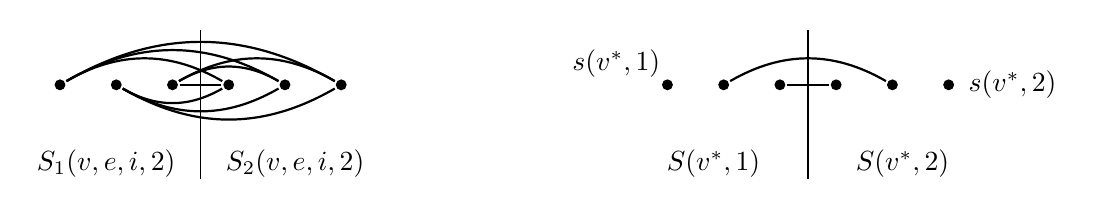
\begin{tikzpicture}[scale=1]
            \begin{scope}[shift={(0cm,0)}]
                %\draw[help lines] (0,-5) grid (12,5);
                \GraphInit[unit=3,vstyle=Normal]
                \SetVertexNormal[Shape=circle, FillColor=black, MinSize=2pt]
                \tikzset{VertexStyle/.append style = {inner sep = \inners, outer sep = \outers}}
                \pgfmathtruncatemacro{\zero}{0}
                \pgfmathtruncatemacro{\one}{1}
                \pgfmathtruncatemacro{\six}{6}
                    \foreach \w in {1} {
                        \foreach \x in {0,1} {
                            \foreach \y in {1,2,3,4,5,6} {
                                \pgfmathsetmacro{\bla}{(6.0 + 12.0/7.0) * \x + 5.0/7.0 * \y}
                                \pgfmathsetmacro{\bly}{-3 * \w}
                                \pgfmathtruncatemacro{\wo}{\w + 1}
                                \ifnum\x=\zero
                                    \Vertex[x=\bla, y=\bly, NoLabel]{e\w\x\y}
                                \else
                                    \ifnum\y=\one
                                        \Vertex[x=\bla, y=\bly, Math, LabelOut, Ldist=-4pt,Lpos=135,L={s(v^*, 1)}]{e\w\x\y}
                                    \else
                                        \ifnum\y=\six
                                          \Vertex[x=\bla, y=\bly, Math, LabelOut, Ldist=1pt,Lpos=0,L={s(v^*, 2)}]{e\w\x\y}
                                        \else
                                            \Vertex[x=\bla, y=\bly, NoLabel]{e\w\x\y}
                                        \fi
                                    \fi
                                \fi
                            }
                            \pgfmathsetmacro{\bla}{2.5 + (6.0 + 12.0/7.0) * \x}
                            \pgfmathsetmacro{\blam}{\bla - 1.2}
                            \pgfmathsetmacro{\blap}{\bla + 1.2}
                            \ifnum\w=\zero
                                \draw (\bla,-0.7) -- (\bla,1.2);
                            \else
                                \draw (\bla,-4.2) -- (\bla,-2.3);
                            \fi
                            \ifnum\w=\zero
                                \ifnum\x=\zero
                                    \node at (\blam,1) {$S_1(v, e, i, 1)$};
                                    \node at (\blap,1) {$S_2(v, e, i, 1)$};
                                \else
                                    \node at (\blam,1) {$S_1(v^*, 1)$};
                                    \node at (\blap,1) {$S_2(v^*, 1)$};
                                \fi
                            \else
                                \ifnum\x=\zero
                                    \node at (\blam,-4) {$S_1(v, e, i, 2)$};
                                    \node at (\blap,-4) {$S_2(v, e, i, 2)$};
                                \else
                                    \node at (\blam,-4) {$S(v^*, 1)$};
                                    \node at (\blap,-4) {$S(v^*, 2)$};
                                \fi
                            \fi
                        }
                    \foreach \z in {4,5,6} {
                        \Edge[style = bend left](e\w01)(e\w0\z)
                        \Edge[style = bend right](e\w02)(e\w0\z)
                    }
                    \Edge(e\w03)(e\w04)
                    \Edge[style = bend left](e\w03)(e\w05)
                    \Edge[style = bend left](e\w03)(e\w06)
                    \Edge[style = bend left](e\w12)(e\w15)
                    \Edge(e\w13)(e\w14)
                }
            \end{scope}
        \end{tikzpicture}
        \caption{\centering Relationships between exterior vertices of a vertex gadget ($d=3$).\label{fig:vert_relations}}
    \end{figure}

    For each color $i \in [2]$, add a $(d, n + 2m)$-spool to $G$, where $n = |V(\mathcal{H})|$ and $m = |E(\mathcal{H})|$.
    Much like the exterior vertices of the vertex gadgets, we attribute unique labels: $C(v, i)$, for each $v \in V(\mathcal{H})$, and $C(e, i, j)$, for each $e \in E(\mathcal{H})$ and $j \in [2]$.
    Now, split the remaining vertices of each labeled set into two equal-sized parts $C_1(\cdot), C_2(\cdot)$ and label one vertex of each $C_{\ell}(e, i, j)$ with the label $c_{\ell}(e, i, j)$ and one of each $C_{\ell}(v, i)$ with $c_{\ell}(v,i)$.
    To conclude, add all edges from $c_{\ell}(v, i)$ to $C_{\ell}(v, i)$, add the edge $c_{\ell}(v, i)c_{3-\ell}(v, i)$, make each $C_{\ell}(e, i, j) \setminus \{c_{\ell}(e, i, j)\}$ into a clique, and, between $C_{\ell}(e, i, j) \setminus \{c_{\ell}(e, i, j)\}$ and $C_r(e, i, k) \setminus \{c_r(e, i, k)\}$, add edges to form a perfect matching, for $\ell,j,r,k \in [2]$.
    That is, each $C_{\ell}(e, i, j)$ forms a perfect matching with three other sets of exterior vertices.
    So far, each $c_{\ell}(v, i)$ has degree $(d+1) + (d-1) + 1 = 2d+1$, other vertices of $C_{\ell}(v, i)$ have degree $d+2$, each vertex in $C_{\ell}(e, i, j) \setminus \{c_{\ell}(e, i, j)\}$ has degree $(d + 1) + (d - 2) + 3 = 2d + 2$, and each vertex labeled $c_{\ell}(e, i, j)$ has degree $d + 1$.

    We now add edges between vertices of different color gadgets.
    In particular, we add every edge between $C_1(v, 2) \setminus \{c_1(v, 2)\}$ and $C_2(v, 1) \setminus \{c_2(v, 1)\}$.
    This increases the degree of these vertices to $2d+1$.
    An example when $d=3$ is illustrated in Figure~\ref{fig:color_relations}.

    \begin{figure}[!htb]
        \centering
        \hspace*{-1cm}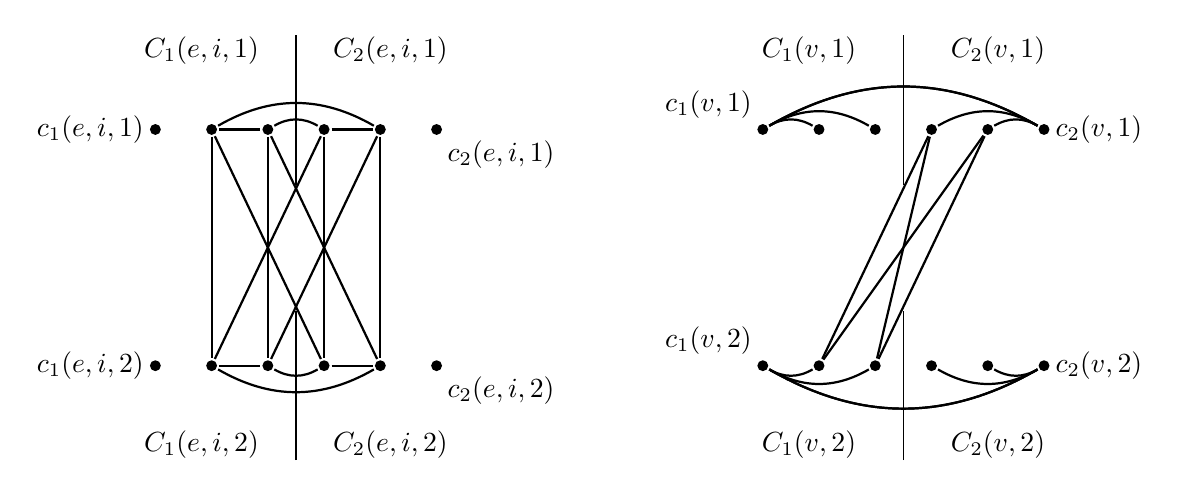
\begin{tikzpicture}[scale=1]
            \begin{scope}[shift={(0cm,0)}]
                %\draw[help lines] (0,-5) grid (12,5);
                \GraphInit[unit=3,vstyle=Normal]
                \SetVertexNormal[Shape=circle, FillColor=black, MinSize=2pt]
                \tikzset{VertexStyle/.append style = {inner sep = \inners, outer sep = \outers}}
                \pgfmathtruncatemacro{\zero}{0}
                \pgfmathtruncatemacro{\one}{1}
                \pgfmathtruncatemacro{\six}{6}
                    \foreach \w in {0, 1} {
                        \foreach \x in {0,1} {
                            \foreach \y in {1,2,3,4,5,6} {
                                \pgfmathsetmacro{\bla}{(6.0 + 12.0/7.0) * \x + 5.0/7.0 * \y}
                                \pgfmathsetmacro{\bly}{-3 * \w}
                                \pgfmathtruncatemacro{\wo}{\w + 1}
                                \ifnum\x=\zero
                                   \ifnum\y=\one
                                    \Vertex[x=\bla, y=\bly, Math, LabelOut, Lpos=180, Ldist=-2pt, L={c_1(e,i,\wo)}]{e\w\x\y}
                                   \else
                                       \ifnum\y=\six
                                           \Vertex[x=\bla, y=\bly, Math, LabelOut, Lpos=-45, Ldist=-2pt, L={c_2(e,i,\wo)}]{e\w\x\y}
                                       \else
                                        \Vertex[x=\bla, y=\bly, NoLabel]{e\w\x\y}
                                       \fi
                                    \fi
                                \else
                                    \ifnum\w=\one
                                       \ifnum\y=\one
                                        \Vertex[x=\bla, y=\bly, Math, LabelOut, Lpos=135, Ldist=-2pt, L={c_1(v,2)}]{e\w\x\y}
                                       \else
                                           \ifnum\y=\six
                                               \Vertex[x=\bla, y=\bly, Math, LabelOut, Lpos=0, Ldist=-2pt, L={c_{2}(v, 2)}]{e\w\x\y}
                                           \else
                                            \Vertex[x=\bla, y=\bly, NoLabel]{e\w\x\y}
                                           \fi
                                        \fi
                                    \else
                                        \ifnum\y=\one
                                        \Vertex[x=\bla, y=\bly, Math, LabelOut, Lpos=135, Ldist=-2pt, L={c_1(v,1)}]{e\w\x\y}
                                       \else
                                           \ifnum\y=\six
                                               \Vertex[x=\bla, y=\bly, Math, LabelOut, Lpos=0, Ldist=-2pt, L={c_{2}(v, 1)}]{e\w\x\y}
                                           \else
                                            \Vertex[x=\bla, y=\bly, NoLabel]{e\w\x\y}
                                           \fi
                                        \fi
                                    \fi
                                \fi
                            }
                            \ifnum\x=\zero
                                \Edge(e\w\x2)(e\w\x3)
                                \Edge(e\w\x4)(e\w\x5)
                                \ifnum\w=\zero
                                    \Edge[style=bend left](e\w\x2)(e\w\x5)
                                    \Edge[style=bend left](e\w\x3)(e\w\x4)
                                \else
                                    \Edge[style=bend right](e\w\x2)(e\w\x5)
                                    \Edge[style=bend right](e\w\x3)(e\w\x4)
                                \fi
                            \else
                                \newcommand{\bla}{right}
                                \ifnum\w=\zero
                                    \renewcommand{\bla}{left}
                                \fi

                                \foreach \y in {2,3} {
                                    \pgfmathtruncatemacro{\z}{7 - \y}
                                    \Edge[style=bend \bla](e\w\x1)(e\w\x\y)
                                    \Edge[style=bend \bla](e\w\x\z)(e\w\x6)
                                    \Edge[style=bend \bla](e\w\x1)(e\w\x6)
                                }
                            \fi
                            \pgfmathsetmacro{\bla}{2.5 + (6.0 + 12.0/7.0) * \x}
                            \pgfmathsetmacro{\blam}{\bla - 1.2}
                            \pgfmathsetmacro{\blap}{\bla + 1.2}
                            \ifnum\w=\zero
                                \draw (\bla,-0.7) -- (\bla,1.2);
                            \else
                                \draw (\bla,-4.2) -- (\bla,-2.3);
                            \fi
                            \ifnum\w=\zero
                                \ifnum\x=\zero
                                    \node at (\blam,1) {$C_1(e, i, 1)$};
                                    \node at (\blap,1) {$C_2(e, i, 1)$};
                                \else
                                    \node at (\blam,1) {$C_1(v, 1)$};
                                    \node at (\blap,1) {$C_2(v, 1)$};
                                \fi
                            \else
                                \ifnum\x=\zero
                                    \node at (\blam,-4) {$C_1(e, i, 2)$};
                                    \node at (\blap,-4) {$C_2(e, i, 2)$};
                                \else
                                    \node at (\blam,-4) {$C_1(v, 2)$};
                                    \node at (\blap,-4) {$C_2(v, 2)$};
                                \fi
                            \fi
                        }
                }
                \foreach \y in {2,3,4,5} {
                    \Edge(e00\y)(e10\y)
                }
                \foreach \y in {2,3} {
                    \pgfmathtruncatemacro{\yp}{\y+2}
                    \pgfmathtruncatemacro{\ym}{7 - \y}
                    \Edge(e00\y)(e10\yp)
                    \Edge(e10\y)(e00\yp)
                    \foreach \z in {4,5} {
                        \Edge(e11\y)(e01\z)
                    }
                }
            \end{scope}
        \end{tikzpicture}
        \caption{\centering Relationships between exterior vertices of color gadgets ($d=3$).\label{fig:color_relations}}
    \end{figure}

    As a first step to connect color gadgets and vertex gadgets, we add every edge between $s(v^*, i)$ and $C_i(v, i)$, every edge between $S(v^*, i) \setminus \{s(v^*, i)\}$ and $C_i(v, i) \setminus \{c_{i}(v, i)\}$, a perfect matching between $S(v^*, i) \setminus \{s(v^*, i)\}$ and $C_{3-i}(v, i) \setminus \{c_{3-i}(v, i)\}$, and the edge $s(v^*, i)c_i(v, 3-i)$.
    Note that this last edge is fundamental, not only because it increases the degrees to the desired value, but also because, if both color gadgets belong to the same side of the cut, every $s(v^*, i)$ will have the same color and, since spools are monochromatic, so would be the {\sl entire} graph, as discussed in more detail below.
    Also note that, aside from $s(v^*, i)$, no other vertex has more than $d$ neighbors outside of its spool.
    The edges described in this paragraph increase the degree of every $s(v^*, i)$ by $d + 1$, yielding a total degree of $2d+2$, of every vertex in $S(v^*, i) \setminus \{s(v^*, i)\}$ to $(d+2) + (d-1) + 1 = 2d+2$, of every vertex in $C_{i}(v, i) \setminus \{c_i(v, i)\}$ to $(d+2) + d = 2d+2$, of every vertex in $C_{i}(v, 3-i) \setminus \{c_i(v, 3-i)\}$ to $(2d+1) + 1 = 2d+2$, and of every $c_{\ell}(v, i)$ to $(2d+1) + 1 = 2d+2$.
    Figure~\ref{fig:color_vertex_relations} gives an example of these connections.


    \begin{figure}[!htb]
        \centering
        \hspace*{-1cm}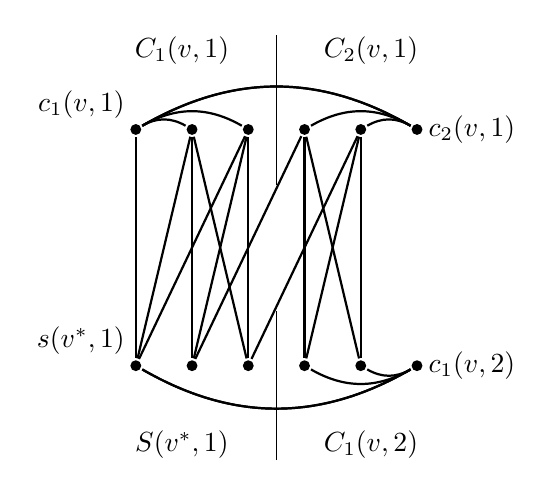
\begin{tikzpicture}[scale=1]
            \begin{scope}[shift={(0cm,0)}]
                %\draw[help lines] (0,-5) grid (12,5);
                \GraphInit[unit=3,vstyle=Normal]
                \SetVertexNormal[Shape=circle, FillColor=black, MinSize=2pt]
                \tikzset{VertexStyle/.append style = {inner sep = \inners, outer sep = \outers}}
                \pgfmathtruncatemacro{\zero}{0}
                \pgfmathtruncatemacro{\one}{1}
                \pgfmathtruncatemacro{\six}{6}
                    \foreach \w in {0, 1} {
                        \foreach \x in {1} {
                            \foreach \y in {1,2,3,4,5,6} {
                                \pgfmathsetmacro{\bla}{(6.0 + 12.0/7.0) * \x + 5.0/7.0 * \y}
                                \pgfmathsetmacro{\bly}{-3 * \w}
                                \pgfmathtruncatemacro{\wo}{\w + 1}
                                \ifnum\x=\zero
                                \else
                                    \ifnum\w=\one
                                       \ifnum\y=\one
                                        \Vertex[x=\bla, y=\bly, Math, LabelOut, Lpos=135, Ldist=-2pt, L={s(v^*,1)}]{e\w\x\y}
                                       \else
                                           \ifnum\y=\six
                                               \Vertex[x=\bla, y=\bly, Math, LabelOut, Lpos=0, Ldist=-2pt, L={c_{1}(v, 2)}]{e\w\x\y}
                                           \else
                                            \Vertex[x=\bla, y=\bly, NoLabel]{e\w\x\y}
                                           \fi
                                        \fi
                                    \else
                                        \ifnum\y=\one
                                        \Vertex[x=\bla, y=\bly, Math, LabelOut, Lpos=135, Ldist=-2pt, L={c_1(v,1)}]{e\w\x\y}
                                       \else
                                           \ifnum\y=\six
                                               \Vertex[x=\bla, y=\bly, Math, LabelOut, Lpos=0, Ldist=-2pt, L={c_{2}(v, 1)}]{e\w\x\y}
                                           \else
                                            \Vertex[x=\bla, y=\bly, NoLabel]{e\w\x\y}
                                           \fi
                                        \fi
                                    \fi
                                \fi
                            }
                            \ifnum\x=\zero
                                \Edge(e\w\x2)(e\w\x3)
                                \Edge(e\w\x4)(e\w\x5)
                                \ifnum\w=\zero
                                    \Edge[style=bend left](e\w\x2)(e\w\x5)
                                    \Edge[style=bend left](e\w\x3)(e\w\x4)
                                \else
                                    \Edge[style=bend right](e\w\x2)(e\w\x5)
                                    \Edge[style=bend right](e\w\x3)(e\w\x4)
                                \fi
                            \else
                                \newcommand{\bla}{right}
                                \ifnum\w=\zero
                                    \renewcommand{\bla}{left}
                                \fi
                                 \foreach \y in {2,3} {
                                     \pgfmathtruncatemacro{\z}{7 - \y}
                                     \ifnum\w=\zero
                                         \Edge[style=bend \bla](e\w\x1)(e\w\x\y)
                                     \fi
                                    \Edge[style=bend \bla](e\w\x1)(e\w\x6)
                                     \Edge[style=bend \bla](e\w\x\z)(e\w\x6)
                                 }
                            \fi
                            \pgfmathsetmacro{\bla}{2.5 + (6.0 + 12.0/7.0) * \x}
                            \pgfmathsetmacro{\blam}{\bla - 1.2}
                            \pgfmathsetmacro{\blap}{\bla + 1.2}
                            \ifnum\w=\zero
                                \draw (\bla,-0.7) -- (\bla,1.2);
                            \else
                                \draw (\bla,-4.2) -- (\bla,-2.3);
                            \fi
                            \ifnum\w=\zero
                                \ifnum\x=\zero
                                \else
                                    \node at (\blam,1) {$C_1(v, 1)$};
                                    \node at (\blap,1) {$C_2(v, 1)$};
                                \fi
                            \else
                                \ifnum\x=\zero
                                \else
                                    \node at (\blam,-4) {$S(v^*, 1)$};
                                    \node at (\blap,-4) {$C_1(v, 2)$};
                                \fi
                            \fi
                        }
                }
                \Edge(e111)(e011)
                \foreach \y in {1,2,3} {
                    \foreach \z in {2,3} {
                        \Edge(e11\y)(e01\z)
                    }
                }
                \foreach \y in {4,5} {
                    \pgfmathtruncatemacro{\ym}{\y - 2}
                    \Edge(e11\ym)(e01\y)
                    \foreach \z in {4,5} {
                        \Edge(e11\y)(e01\z)
                    }
                }
            \end{scope}
        \end{tikzpicture}
        \caption{\centering Relationships between exterior vertices of color and vertex gadgets ($d=3$).\label{fig:color_vertex_relations}}
    \end{figure}



    For the final group of gadgets, namely hyperedge gadgets, for each $\{x, y, z\} \in E(\mathcal{H})$, each color $i$, and each pair $j,\ell \in [2]$, we add one additional vertex $c_{\ell}'(e, i, j)$ adjacent to $c_{\ell}(e, i, j)$, $S_{\ell}(x, e, i, j)$, $S_{\ell}(y, e, i , j)$, and $c_{3-\ell}'(e, i, j)$; finally, we add every edge between $c_{\ell}(e, i, j)$ and $S_{\ell}(z, e, i ,j)$. See Figure~\ref{fig:hyper_relations} for an illustration.
    Note that $c_{\ell}'(e, i, j)$ has degree $2d + 2$; the degree of $c_{\ell}(e, i ,j)$ increased from $d + 1$ to $2d + 2$, and the degree of each vertex of $S_{\ell}(x, e, i, j)$ increased from $2d + 1$ to $2d + 2$.
    This concludes our construction of the $(2d + 2)$-regular graph $G$.

    \begin{figure}[!htb]
        \centering
        \hspace*{-0.25cm}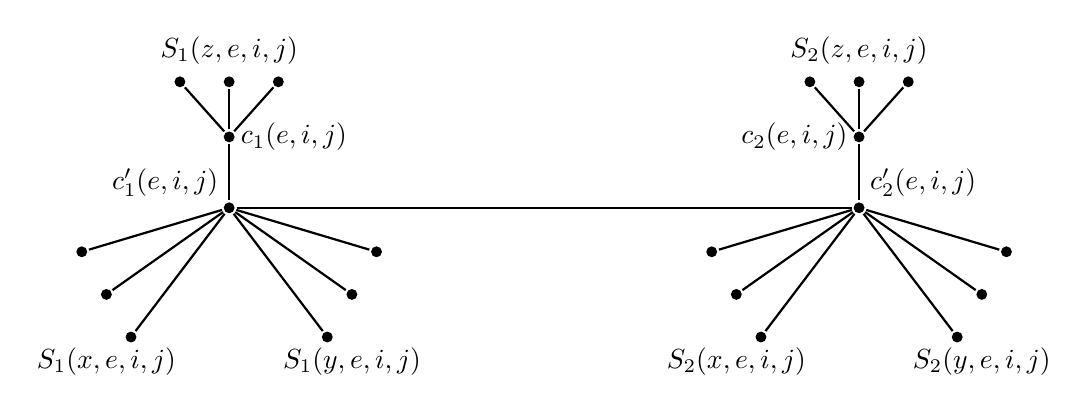
\begin{tikzpicture}[scale=1]
            \begin{scope}[shift={(0cm,0)}]
                %\draw[help lines] (0,-5) grid (12,5);
                \GraphInit[unit=3,vstyle=Normal]
                \SetVertexNormal[Shape=circle, FillColor=black, MinSize=2pt]
                \tikzset{VertexStyle/.append style = {inner sep = \inners, outer sep = \outers}}
                \pgfmathtruncatemacro{\zero}{0}
                \pgfmathtruncatemacro{\one}{1}
                \pgfmathtruncatemacro{\six}{6}
                \foreach \x in {0,1} {
                    \pgfmathtruncatemacro{\sh}{(6.29 + 12.0/7.0) * \x}
                    \begin{scope}[shift={(\sh,0)}]
                        \pgfmathtruncatemacro{\xp}{1 + 1*\x}
                        \pgfmathtruncatemacro{\pe}{180*(\x)}
                        \pgfmathtruncatemacro{\pep}{45 + 90*(1-\x)}
                        \Vertex[x=0, y=1.1, Math, LabelOut, Ldist=-2pt,Lpos=\pe,L={c_\xp(e,i,j)}]{e\x}
                        \Vertex[x=0, y=0.2, Math, LabelOut, Ldist=-2pt,Lpos=\pep,L={c'_\xp(e,i,j)}]{ep\x}
                        \Edge(e\x)(ep\x)
                        \foreach \w in {0,1,2} {
                            \pgfmathsetmacro{\ang}{120*(\w+1)}
                            \begin{scope}[rotate=\ang]
                                \foreach \y in {1,2,3} {
                                    \pgfmathsetmacro{\gap}{5.0/8.0}
                                    \pgfmathsetmacro{\bla}{\gap * \y - 2*\gap}
                                    \pgfmathtruncatemacro{\ym}{\y - 1}
                                    \newcommand{\setname}{z}
                                    \newcommand{\lpos}{270}
                                    \newcommand{\ldist}{13pt}
                                    \ifnum\w>\one
                                        \renewcommand{\lpos}{90}
                                        \renewcommand{\ldist}{0pt}
                                    \fi
                                    \ifnum\w=\zero
                                        \renewcommand{\setname}{x}
                                    \fi
                                    \ifnum\w=\one
                                        \renewcommand{\setname}{y}
                                    \fi
                                    \ifnum\ym=\one
                                        \Vertex[x=\bla, y=1.8, Math, LabelOut, Lpos=\lpos, Ldist=\ldist, L={S_{\xp}(\setname, e, i, j)}]{e\w\x\y}
                                    \else
                                        \Vertex[x=\bla, y=1.8, NoLabel]{e\w\x\y}
                                    \fi
                                    \ifnum\w>\one
                                        \Edge(e\x)(e\w\x\y)
                                    \else
                                        \Edge(ep\x)(e\w\x\y)
                                    \fi
                                }
                            \end{scope}
                        }
                    \end{scope}
                }
                \Edge(ep0)(ep1)
            \end{scope}
        \end{tikzpicture}
        \caption{\centering Hyperedge gadget ($d=3$).\label{fig:hyper_relations}}
    \end{figure}

    Now, suppose we are given a valid bicoloring $\varphi$ of $\mathcal{H}$, and our goal is to construct a $d$-cut $(A, B)$ of $G$. Put the gadget of color 1 in $A$ and the other one in $B$.
    For each vertex $v \in V(\mathcal{H})$, if $\varphi(v) = 1$, put the gadget corresponding to $v$ in $A$, otherwise put it in $B$.
    In the interface between these gadgets, no vertex from the color gadgets has more than $d$ neighbors in a single vertex gadget, therefore none violates the $d$-cut property.
    As to the vertices coming from the vertex gadgets, only $s_{\ell}(v^*, i)$ has more than $d$ neighbors outside of its gadget; however, it has $d$ neighbors in the color gadget for color $i$ and only one in color $3-i$.
    Since each color gadget is in a different side of the partition, $s_{\ell}(v^*, i)$ does not violate the degree constraint.
    For each hyperedge $e = \{x, y, z\}$, put $c_{\ell}'(e, i, j)$ in the same set as the majority of its neighbors, this way, it will not violate the property -- note that its other neighbor, $c_{3-\ell}'(e, i , j)$, will be in the same set because it will have the exact same amount of vertices on each side of the partition in its neighborhood.
    So, if $\varphi(x) = \varphi(y) = 1$, $c_{\ell}'(e, i, j) \in A$; however, since $e$ is not monochromatic, $\varphi(z) = 2$, so $c_{\ell}(e, i ,j)$ has at most $d$ neighbors in the other set.
    The case where $\varphi(x) \neq \varphi(y)$ is similar.
    Thus, we conclude that $(A, B)$ is indeed a $d$-cut of $G$.


    Conversely, take a $d$-cut $(A, B)$ of $G$ and construct a bicoloring of $\mathcal{H}$ such that $\varphi(v) = 1$ if and only if the spool corresponding to $v$ is in $A$.
    Suppose that this process results in some hyperedge $e = \{x, y, z\} \in E(\mathcal{H})$ begin monochromatic.
    That is, there is some hyperedge gadget where $S_{\ell}(x, e, i, j)$, $S_{\ell}(y, e, i, j)$, and $S_{\ell}(z, e, i, j)$ are in $A$, which implies that $c_{\ell}'(e, i, j) \in A$ and, consequently, that $c_{\ell}(e, i, j) \in A$ for every $\ell,i,j \in [2]$.
    However, since $c_{\ell}(e, 1, j)$ and $c_{\ell}(e, 2, j)$ are in $A$ and a color gadget is monochromatic, both color gadgets belong to $A$, which in turn implies that every $s(v^*, i)$ has $d+1$ neighbors in $A$ and, therefore, must also be in $A$ by Observation~\ref{obs:mono_bipartite}.
    Moreover, since spools are monochromatic, every vertex gadget is in $A$, implying that the entire graph belongs to $A$, contradicting the hypothesis that $(A, B)$ is a $d$-cut of $G$.
\end{proof}


The graphs constructed by the above reduction are neither planar nor bipartite, but they are regular, a result that we were unable to find in the literature for \pname{Matching Cut}.
Note that every planar graph has a $d$-cut for every $d \geq 5$, so only the cases $d \in \{2,3,4\}$ remain open, as the case $d=1$ is known to be $\NP$-hard~\cite{matching_cut_planar}. % \ig{check $d=4$!!}.
%and as such, we do not expect \ig{why?} the $\NP$-hardness results for planar graphs to be easily adapted to \textsc{$d$-Cut} when $d \in \{2,3,4\}$.
%Using the same arguments, and in fact
Concerning graphs of bounded diameter, Le and Le~\cite{matching_cut_diameter} prove the $\NP$-hardness of \textsc{Matching Cut} for graphs of diameter at least three by reducing \textsc{Matching Cut} to itself.  It can be easily seen that the same construction given by Le and Le~\cite{matching_cut_diameter}, but reducing  \pname{$d$-Cut} to itself, also proves the $\NP$-hardness of \pname{$d$-Cut} for every $d \geq 1$. %\ig{I changed the following to ``corollary''}

%., we also conclude that \pname{$d$-Cut} is $\NP$-hard for graphs of diameter at least three.

\begin{corollary}
    For every integer $d \geq 1$, \pname{$d$-Cut} is $\NP$-hard for graphs of diameter at least three.
\end{corollary}

We leave as an open problem to determine whether there exists a  polynomial-time algorithm for \pname{$d$-Cut} for graphs of diameter at most two for every $d \geq 2$, as it is the case for $d=1$~\cite{matching_cut_diameter}.


%We leave questions regarding specific graph classes as open problems and focus on the general case \ig{not really true, as the next theorem focuses on graphs of bounded degree...}.


\subsection{Polynomial algorithm for graphs of bounded degree}
\label{sec:poly-algo}


Our next result is a natural generalization of Chvátal's algorithm~\cite{chvatal_matching_cut} for \pname{Matching Cut} on graphs of maximum degree three.

\begin{theorem}
    \label{thm:small_deg_poly}
    For any graph $G$ and integer $d \geq 1$ such that $\Delta(G) \leq d+2$, it can be decided in polynomial time if $G$ has a $d$-cut. Moreover, for $d=1$ any graph $G$ with $\Delta(G) \leq 3$ and $|V(G)| \geq 8$ has a matching cut, for $d=2$ any graph $G$ with $\Delta(G) \leq 4$ and $|V(G)| \geq 6$ has a $2$-cut, and for $d\geq 3$ any graph $G$ with $\Delta(G) \leq d+2$ has a $d$-cut.
\end{theorem}

\begin{proof}
    We may assume that $G$ is connected, as otherwise it always admits a $d$-cut. If $G$ is a tree, any edge is a cut edge and, consequently, a $d$-cut is easily found.
    So let $C$ be a shortest cycle of $G$.
    If $d = 1$ we use Chvátal's result~\cite{chvatal_matching_cut} together with the size bound of eight observed by Moshi~\cite{matching_cut_moshi}; hence, we may assume that $d \geq 2$.
    In the case that $V(G) = C$, we may pick any vertex $v$ and note that $(\{v\}, C \setminus \{v\})$ is a $d$-cut.

   % \ig{I restructured the distinction of cases}

     Suppose first that $|C| = 3$ and $d = 2$.  If $(C, V(G) \setminus C)$ is a $2$-cut, we are done. Otherwise, there is some vertex $v \notin C$ with three neighbors in $C$ (since by the hypothesis on $\Delta(G)$, every vertex in $C$ has at most two neighbors in $G - C$) and, consequently, $Q := C \cup \{v\}$ induces a $K_4$.
    If $V(G) = Q$, we can arbitrarily partition $Q$ into two sets with two vertices each and get a $2$-cut of $G$.
    Also, if no other $u \notin Q$ has three neighbors in $Q$, $(Q, V(G) \setminus Q)$ is a $2$-cut of $G$.
    If there is such a vertex $u$, let $R := Q \cup \{u\}$. If $V(G) = R$, then clearly $G$ has no $2$-cut. Note that $|Q|=5$, and this will be the only case in the proof where $G$ does not have a $d$-cut. Otherwise, if $V(G) \neq R$, $(R, V(G) \setminus R)$ is a $2$-cut, because no vertex outside of $R$ can be adjacent to more than two vertices in $R$, and we are done.

    If $|C| = 3$ and $d \geq 3$, then clearly $(C, V(G) \setminus C)$ is a $d$-cut, and we are also done.

    Otherwise, that is, if $|C| \geq 4$, we claim that $(C, V(G) \setminus C)$ is always a $d$-cut.
    For $v \in C$, note that $\dgr(v) \leq d + 2$, hence $v$ has at most $d$ neighbors in $G - C$. For $v \in V(G) \setminus C$, if $|C| \geq 5$, necessarily $\dgr_C(v) \leq 1$, as otherwise we would find a cycle in $G$ shorter than $C$, and therefore $(C, V(G) \setminus C)$ is a $d$-cut.
    By a similar argument, if $|C| = 4$, then $\dgr_C(v) \leq 2$, and the theorem follows as we assume that $d \geq 2$.
    %The only other case where we would not shorten $C$ is when $|C| = 3$ and $d \geq 3$, but trivially $(C, V(G) \setminus C)$ is a $3$-cut of $G$.
\end{proof}

Theorems~\ref{thm:regular_nph} and~\ref{thm:small_deg_poly} present a ``quasi-dichotomy'' for $d$-cut on graphs of bounded maximum degree.
Specifically, for $\Delta(G) \in \{d+3, \dots, 2d+1\}$, the complexity of the problem remains unknown.
However, we believe that most, if not all, of these open cases can be solved in polynomial time; see the discussion in Section~\ref{sec:concl}.


\subsection{Exact exponential algorithm}
\label{sec:exact-algo}

To conclude this section, we present a simple exact exponential algorithm which, for every $d \geq 1$, runs in time $\bigOs{c_d^n}$ for some constant $c_d < 2$.
For the case $d=1$, the currently known algorithms~\cite{matching_cut_tcs,matching_cut_ipec} exploit structures that appear to get out of control when $d$ increases, and so has a better running time than the one described below.

When an instance of size $n$ branches into $t$ subproblems of sizes at most $n - s_1, \dots, n - s_t$, respectively, the vector $(s_1, \dots, s_t)$ is called the \tdef{branching vector} of this branching rule, and the unique positive real root of the equation $x^n - \sum_{i \in [t]} x^{n - s_i} = 0$ is called the \tdef{branching factor} of the rule.
The total complexity of a branching algorithm is given by $\bigOs{\alpha^n}$, where $\alpha$ is the largest branching factor among all rules of the algorithm.
For more on branching algorithms, we refer to~\cite{exact_exponential_algorithms}.

\begin{theorem}
    For every fixed integer $d \geq 1$ and $n$-vertex graph $G$, there is an algorithm that solves \pname{$d$-Cut} in time $\bigOs{c_d^n}$, for some constant $1 < c_d < 2$.
\end{theorem}

\begin{proof}
    Our algorithm takes as input $G$ and outputs a $d$-cut $(A, B)$ of $G$, if it exists.
    To do so, we build a branching algorithm that maintains, at every step, a tripartition of $V(G) = A \dot\cup B \dot\cup D$ such that $(A, B)$ is a $d$-cut of $G \setminus D$.
    The central idea of our rules is to branch on small  sets of vertices (namely, of size at most $d+1$) at each step such that either at least one bipartition of the set forces some other vertex to choose a side of the cut, or we can conclude that there is at least one bipartition that violates the $d$-cut property.
    First, we present our reduction rules, which are applied following this order at the beginning of each recursive step.

    \begin{itemize}
        \item[R1] If $(A, B)$ violates the $d$-cut property, output $\NOi$.
        \item[R2] If $D = \emptyset$, we have a $d$-cut of $G$. Output $(A,B)$.
        \item[R3] If there is some $v \in D$ with $\dgr_A(v) \geq d + 1$ and $\dgr_B(v) \geq d+1$, output $\NOi$.
        \item[R4] While there is some $v \in D$ with $\dgr_A(v) \geq d + 1$ (resp. $\dgr_B(v) \geq d+1$), add $v$ to $A$ (resp. $B$).
    \end{itemize}

    Our branching rules, and their respective branching vectors, are listed below.

    \begin{itemize}
        \item[B1] If there is some $v \in A \cup B$ with $\dgr_D(v) \geq d+1$, choose a set $X \subseteq N_D(v)$ of size $d$ and branch on all possible possible bipartitions of $X$.
        Note that, if all vertices of $X$ are in the other side of $v$, at least one vertex of $N_D(v) \setminus X$ must be in the same side as $v$.
        As such, this branching vector is of the form $\{d+1\} \times \{d\}^{2^d-1}$.


        %\item[B2] If there exists $v \in D$ with $d_D(v) \geq d+1$, choose a set $X \subseteq N_D(v)$ of size $d+1$ and branch on all possible possible bipartitions of $X$.
        %For the branching vector, we have that, if $X \subseteq A$ or $X \subseteq B$, $v$ must be on the same side as $X$, otherwise it would violate the $d$-cut property.
        %This yields the vector $\{d+2\}^2 \times \{d+1\}^{2^d}$.
        %
        %\item[B3] If there is some $v \in D$ such that $d_A(v) + d_D(v) \geq d+1$ (resp. $d_B(v) + d_D(v) \geq d+1$), choose a set $X \subseteq N_D(v)$ of size $s = d+1 - d_A(v)$ (resp. $s = d+1 - d_B(v)$) and branch on every possible bipartition of $X$.
        %Since rules R4 and B2 were not applied, we have that $d_D(v) \leq d$, $1 \leq d_A(v) \leq d$ (resp. $1 \leq d_B(v) \leq d$), and $s \geq d$.
        %Now, if $X$ is entirely contained in $A$ (resp. $B$), we have that $v$ must be placed alongside $X$ on a valid $d$-cut that extends $(A, B)$.
        %Therefore, we conclude that this branching vector, in the worst case where $s = d$, is given by $\{d+1\} \times \{d\}^{2^d-1}$.


        \item[B2] If there is some $v \in A$ (resp. $B$) such that $\dgr_B(v) + \dgr_D(v) \geq d+1$ (resp. $\dgr_A(v) + \dgr_D(v) \geq d+1$), choose a set $X \subseteq N_D(v)$ of size $s = d+1 - \dgr_B(v)$ (resp. $s = d+1 - \dgr_A(v)$) and branch on every possible bipartition of $X$.
        Since rule B1 was not applied, we have that $\dgr_D(v) \leq d$, $\dgr_B(v) \geq 1$ (resp. $\dgr_A(v) \geq 1$), and $s \leq d$.
        If all vertices of $X$ were placed in $B$ (resp. $A$), we would violate the $d$-cut property and, thus, do not need to investigate this branch of the search.
        In the worst case, namely when $s = d$, this yields the branching vector $\{d\}^{2^d-1}$.
    \end{itemize}

    We now claim that, if none of the above rules is applicable, we have that $(A \cup D, B)$ is a $d$-cut of $G$.
    To see that this is the case, suppose that there is some vertex $v \in V(G)$ that violates the $d$-cut property; that is, it has a set $Y$ of $d+1$ neighbors across the cut.

    Suppose that $v \in B$. Then $Y \subseteq A \cup D$, so we have $\dgr_A(v) + \dgr_D(v) \geq d+1$, in which case rule B2 could be applied, a contradiction.
    %In this case we know that $Y \nsubseteq A$, as otherwise R1 would have been applied, and that $Y \nsubseteq D$, as otherwise rule B1 would have been applied.
%    Furthermore, $Y \nsubseteq (A \cup D)$, as otherwise we would have $\dgr_A(v) + \dgr_D(v) \geq d+1$, in which case rule B2 would have been applied \ig{isn't this last case enough? Do we need to worry about the order of the rules?}. This contradicts the hypothesis that $v$ violates the $d$-cut property.
    Thus, we have that $v \notin B$, so $Y \subseteq B$ and either $v \in A$ or $v \in D$;
    in the former case, again by rule R1, $(A, B)$ would not be a $d$-cut.
     In the latter case, we would have that $\dgr_B(v) \geq d+1$, but then rule R4 would still be applicable.
    Consequently, $v \notin A \cup B \cup D = V(G)$, so such a vertex does not exist, and thus we have that $(A \cup D, B)$ is a $d$-cut of $G$.
    Note that a symmetric argument holds for the bipartition $(A, B \cup D)$.
    Before executing the above branching algorithm, we need to ensure that $A \neq \emptyset$ and $B \neq \emptyset$.
    To do that, for each possible pair of vertices $u,v \in V(G)$, we execute the entire algorithm starting with $A := \{u\}$ and $B := \{v\}$.

    As to the running time of the algorithm, for rule B2 we have that the unique positive real root of $x^n - (2^d - 1)x^{n - d} = 0$ is of the closed form $x = \sqrt[\leftroot{2}d]{2^d - 1} < 2$.
    For rule B1, we have that the polynomial associated with the recurrence relation, $p_d(x) = x^n - (2^d - 1)x^{n - d} - x^{n - d - 1}$, verifies $p_d(1) = 1 - 2^d < 0$ and $p_d(2) = 2^{n - d - 1} > 0$.
    Since it is a continuous function and $p_d(x)$ has an unique positive real root $c_d$, it holds that $1 < c_d < 2$.
    The final complexity of our algorithm is $\bigOs{c_d^n}$, with $\sqrt[\leftroot{2}d]{2^d - 1} < c_d < 2$, since $p_d\left(\sqrt[\leftroot{2}d]{2^d - 1}\right) = -(2^d - 1)^{\frac{n-d-1}{d}} < 0$.
    Table~\ref{tab:exact_values} presents the branching factors for some values of $d$ for our two branching rules.

\begin{table}[!htb]
    \centering
    \begin{tabular}{c|ccccccc}
         $d$ & 1 & 2 & 3 & 4 & 5 & 6 & 7\\
         \hline
         B1 & 1.6180 & 1.8793 & 1.9583 & 1.9843 & 1.9937 & 1.9973 & 1.9988 \\
         B2 & 1.0000 & 1.7320 & 1.9129 & 1.9679 & 1.9873 & 1.9947 & 1.9977 \\

    \end{tabular}\smallskip
    \caption{\centering Branching factors for some values of $d$.}
    \label{tab:exact_values}
\end{table}
\end{proof} 

\section{Parameterized algorithms and kernelization}
\label{sec:param}

In this section we focus on the parameterized complexity of \textsc{$d$-Cut}. More precisely, in Section~\ref{sec:crossing-edges} we consider as the parameter the number of edges crossing the cut, in Section~\ref{thm:algo-tw} the treewidth of the input graph, in Section~\ref{sec:kernelization} the distance to cluster (in particular, we provide a quadratic kernel), and in Section~\ref{sec:cocluster} the distance to co-cluster.


\subsection{Crossing edges}
\label{sec:crossing-edges}


In this section we consider as the parameter the maximum number of edges crossing the cut. In a nutshell, our approach is to use as a black box one of the algorithms presented by Marx et al.~\cite{marx_treewidth_reduction} for a class of separation problems. Their fundamental problem is \pname{$\mathcal{G}$-MinCut}, for a fixed class of graphs $\mathcal{G}$, which we state formally, along with their main result, below.


\pproblem{$\mathcal{G}$-MinCut}{A graph $G$, vertices $s,t $, and an integer $k$.}{Is there an induced subgraph $H$ of $G$ with at most $k$ vertices such that $H \in \mathcal{G}$ and $H$ is an $s-t$ separator?}{The integer $k$.}{13.5}

\begin{theorem}[Theorem 3.1 in~\cite{marx_treewidth_reduction}]
    \label{thm:marx}
    If $\mathcal{G}$ is a decidable and hereditary graph class, \pname{$\mathcal{G}$-MinCut} is $\FPT$.
\end{theorem}

To be able to apply Theorem~\ref{thm:marx}, we first need to specify a graph class to which, on the line graph, our separators correspond. We must also be careful to guarantee that the removal of a separator in the line graph leaves non-empty components in the input graph. To accomplish that, for each $v \in V(G)$, we add a private clique of size $2d$ adjacent only to it, choose one arbitrary vertex $v'$ in each of them, and our algorithm will ask for the existence of a ``special'' separator of the appropriate size between every pair of chosen vertices of two distinct private cliques. We assume henceforth that these private cliques have been added to the input graph $G$.

For each integer $d \geq 1$, we define the graph class $\mathcal{G}_d$ as follows.

\begin{definition}
    A graph $H$ belongs to $\mathcal{G}_d$ if and only if its maximum clique size is at most $d$.
\end{definition}

Note that $\mathcal{G}_d$ is clearly decidable and hereditary for every integer $d \geq 1$.


\begin{lemma}
    \label{lem:cut_mincut}
    $G$ has a $d$-cut if and only if $L(G)$ has a vertex separator belonging to $\mathcal{G}_d$.
\end{lemma}

\begin{proof}
    Let $H = L(G)$, $(A, B)$ be a $d$-cut of $G$, and $F \subseteq V(H)$ be the set of vertices such that $e_{uv} \in F$ if and only if $u \in A$ and $v \in B$, or vice-versa.
    The fact that $F$ is a separator of $H$ follows directly from the hypothesis that $(A, B)$ is a cut of $G$.
    Now, to show that $H[F] \in \mathcal{G}_d$, suppose for contradiction that $H[F]$ contains a  clique $Q$ with more than $d$ vertices.
    That is, there are at least $d+1$ edges of $G$ that are pairwise intersecting and with one endpoint in $A$ and the other in $B$.
    Note, however, that for at least one of the parts, say $A$, there is also \textit{at most} one vertex with an edge in $Q \subseteq E(G)$, as otherwise there would be two non-adjacent vertices in the clique $Q \subseteq V(H)$.
    As such, $A$ has only one vertex and we conclude that every edge in $Q$ has an endpoint in $A$, but this, on the other hand, implies that $A$ has $d+1$ neighbors in $B$, contradicting the hypothesis that $(A, B)$ is a $d$-cut of $G$.


    For the converse, take a vertex separator $S \subseteq V(H)$ such that $H[S] \in \mathcal{G}_d$ and let $E_S$ be the edges of $G$ corresponding to $S$.
    %Since $s$ and $t$ are edges of a private clique \ig{what are $s$ and $t$? We have never defined them}, for simplicity we use $v_s$ and $v_t$ to denote the respective vertices in $G$.
    Let $G'$ be the graph where each vertex corresponds to a connected component of $G - E_S$ and two vertices are adjacent if and only if there is an edge in $E_S$ between vertices of the respective components.
    Let $Q_r$ be an arbitrarily chosen connected component of $G - E_S$.
    Now, for each component at an odd distance from $Q_r$ in $G'$, add that component to $B$; all other components are placed in $A$.
    We claim that $(A, B)$ is a $d$-cut of $G$. Let $F \subseteq E_S$ be the set of edges with one endpoint in $A$ and the other in $B$.
    Note that $G - F$ is disconnected due to the construction of $A$ and $B$.
    If there is some $v \in A$ with more than $d$ neighbors in $B$, we obtain that there is some clique of equal size in $H[S]$, contradicting the hypothesis that this subgraph belongs to $\mathcal{G}_d$.
\end{proof}




\begin{theorem}\label{thm:FPT-crossing}
    For every $d \geq 1$, there is an $\FPT$ algorithm for \pname{$d$-Cut} parameterized by $k$, the maximum number of edges crossing the cut.
\end{theorem}

\begin{proof}
    For each pair of vertices $s,t \in V(G)$ that do not belong to the private cliques, our goal is to find a subset of vertices $S \subseteq V(L(G))$ of size at most $k$ that separates $s$ and $t$ such that $L(G)[S] \in \mathcal{G}_d$.
    This is precisely what is provided by Theorem~\ref{thm:marx}, and the correctness of this approach is guaranteed by Lemma~\ref{lem:cut_mincut}.
    Since we perform a quadratic number of calls to the  algorithm given by Theorem~\ref{thm:marx}, our algorithm still runs in $\FPT$ time.
\end{proof}

As to the running time of the $\FPT$ algorithm given by Theorem~\ref{thm:FPT-crossing}, the treewidth reduction technique of~\cite{marx_treewidth_reduction} relies on the construction of a monadic second order logic (MSOL) expression and Courcelle's Theorem~\cite{courcelle_theorem} to guarantee fixed-parameter tractability, and therefore it is hard to provide an explicit running time in terms of $k$.

\subsection{Treewidth}
\label{thm:algo-tw}

We proceed to present an algorithm for \pname{$d$-Cut} parameterized by the treewidth of the input graph that, in particular, improves the running time of the best known algorithm for \pname{Matching Cut}~\cite{matching_cut_structural}.
For the definitions of treewidth we refer to~\cite{treewidth,CyganFKLMPPS15}.
We state here an adapted definition of nice tree decomposition which shall be useful in our algorithm.


%A \textit{tree decomposition} of a graph $G$ is defined as $\td{T} = (T, \mathcal{B} = \{B_j \mid j \in V(T)\})$, where $T$ is a tree and $\mathcal{B} \subseteq 2^{V(G)}$ is a family where: $\bigcup_{B_j \in \mathcal{B}} B_j = V(G)$;
%for every edge $uv \in E(G)$ there is some~$B_j$ such that $\{u,v\} \subseteq B_j$;
%for every $i,j,q \in V(T)$, if $q$ is in the path between $i$ and $j$ in $T$, then $B_i \cap B_j \subseteq B_q$.
%Each $B_j \in \mathcal{B}$ is called a \textit{bag} of the tree decomposition.
%The \textit{width} of a tree decomposition is defined as the size of a largest bag minus one.
%The \textit{treewidth} $\tw(G)$ of a graph $G$ is the smallest width among all valid tree decompositions of $G$~\cite{downey_fellows}.
%If $\td{T}$ is a rooted tree, by $G_x$ we will denote the subgraph of $G$ induced by the vertices contained in any bag that belongs to the subtree of $\td{T}$ rooted at bag $x$.
%An algorithmically useful property of tree decompositions is the existence of a so said \textit{nice tree decompositions} of width $\tw(G)$.


\begin{definition}{(Nice tree decomposition)}
    A tree decomposition $(T, \mathcal{B})$ of a graph $G$ is said to be \emph{nice} if it T is a tree rooted at an empty bag $r(T)$ and each of its bags is from one of the following four types:
    \begin{enumerate}
        \item \textit{Leaf node}: a leaf $x$ of $T$ with $|B_x| = 2$ and no children.
        \item \textit{Introduce node}: an inner node $x$ of $T$ with one child $y$ such that $B_x \setminus B_y = \{u\}$, for some $u \in V(G)$.
        \item \textit{Forget node}: an inner node $x$ of $T$ with one child $y$ such that $B_y \setminus B_x = \{u\}$, for some $u \in V(G)$.
        \item \textit{Join node}: an inner node $x$ of $T$ with two children $y,z$ such that $B_x = B_y = B_z$.
    \end{enumerate}
\end{definition}


In the next theorem, note that the assumption that the given tree decomposition is \textit{nice} is not restrictive, as any tree decomposition can be transformed into a nice one of the same width in polynomial time~\cite{Klo94}.

\begin{theorem}\label{thm:treewidth}
    For every integer $d \geq 1$, given a nice tree decomposition of $G$ of width $\tw(G)$, \pname{$d$-Cut} can be solved in time $\bigOs{2^{\tw(G)+1}(d+1)^{2\tw(G) + 2}}$.
\end{theorem}

\begin{proof}
    As expected, we will perform dynamic programming on a nice tree decomposition.
    For this proof, we denote a $d$-cut of $G$ by $(L, R)$ and suppose that we are given a total ordering of the vertices of $G$.
    Let $(T, \mathcal{B})$ be a nice tree decomposition of $G$ rooted at a node $r \in V(T)$.
    For a given node $x \in T$, an entry of our table is indexed by a triple $(A, \balpha, t)$, where $A \subseteq B_x$, $\balpha \in \left(\{0\} \cup [d]\right)^{\tw(G)+1}$, and $t$ is a binary value. Each coordinate $a_i$ of $\alpha$ indicates how many vertices \textit{outside} of $B_x$ the $i$-th vertex of $B_x$ has in the other side of the partition. More precisely, we denote by $f_x(A, \balpha, t)$ the binary value indicating whether or not $V(G_x)$ has a bipartition $(L_x,R_x)$ such that $L_x \cap B_x = A$, every vertex $v_i \in B_x$ has exactly $a_i$ neighbors in the other side of the partition $(L_x,R_x)$  outside of $B_x$, and both $L_x$ and $R_x$ are non-empty if and only if $t = 1$. Note that $G$ admits a $d$-cut if and only if $f_r(\emptyset, \boldsymbol{0}, 1)=1$.
    Figure~\ref{fig:treewidth} gives an example of an entry in the dynamic programming table and the corresponding solution on the subtree.


    % indicating if both $L$ and $R$ are non-empty in $G_x$. \ig{Redefine: there must exist a bipartition $(L_x,R_x)$ of $G_x$ such that $L_x \cap B_x = A$, $\balpha$ captures the degrees on the other side of $(L_x,R_x)$, and $t$ says whether both sides are non-empty. Say that for the root, this indeed solved the problem} Semantically, $A$ represents which vertices of $B_x$ are in $L$, each coordinate $a_i$ of $\alpha$ indicates how many vertices {\sl outside} of $B_x$ the $i$-th vertex of $B_x$ has in the other side of the partition, and $t$ indicates if the condition that both $L$ and $R$ are non-empty in $G_x$ has been satisfied.
%    As such, we denote by $f_x(A, \balpha, t)$ the binary value indicating whether or not $G_x$ has a bipartition such that $A \subseteq L$, vertex $v_i \in B_x$ has $a_i$ neighbors in the other side of the partition outside of $B_x$, and both $L$ and $R$ are non-empty if and only if $t = 1$.

    \begin{figure}[!htb]
        \centering
        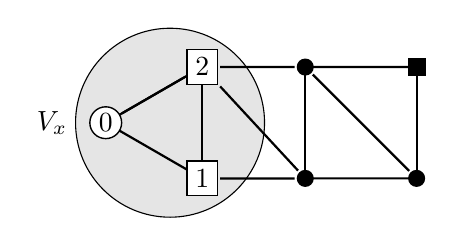
\begin{tikzpicture}[rotate = 90]
                %\draw[help lines] (-5,-5) grid (5,5);
                \GraphInit[unit=3,vstyle=Normal]
                \SetVertexNormal[Shape=circle, MinSize=3pt]
                \tikzset{VertexStyle/.append style = {inner sep = \inners, outer sep = \outers}}
                \SetVertexNoLabel
                \begin{scope}[rotate=90]
                    \draw[fill=gray!20] (0,0) circle (1.2);
                    \node at (1.5, 0) {$V_x$};
                    \grComplete[RA=0.816747, prefix=t]{3}
                    \SetVertexLabel
                    \Vertex[Node, L = {0}, Math]{t0}
                \end{scope}
                \begin{scope}[rotate=90]
                    \tikzset{VertexStyle/.append style = {inner sep = 3pt, shape = rectangle}}
                    \SetVertexLabel
                    \Vertex[Node, L = {2}, Math]{t2}
                    \Vertex[Node, L = {1}, Math]{t1}
                \end{scope}
                \begin{scope}[rotate=45, shift={(-1.71424, -1.71424)}]
                    \grCycle[RA=1, prefix=c]{4}
                    \Edge(t0)(t2)
                \end{scope}
                \begin{scope}[rotate=45, shift={(-1.71424, -1.71424)}]
                    \SetVertexNormal[Shape=circle, FillColor = black, MinSize=3pt]
                    \tikzset{VertexStyle/.append style = {shape = rectangle, inner sep = 3pt, outer sep = \outers}}
                    \Vertex[Node]{c3}
                \end{scope}
                \begin{scope}[rotate=45, shift={(-1.71424, -1.71424)}]
                    \SetVertexNormal[Shape=circle, FillColor = black, MinSize=3pt]
                    \tikzset{VertexStyle/.append style = {inner sep = 2pt, outer sep = \outers}}
                    \Vertex[Node]{c0}
                    \Vertex[Node]{c1}
                    \Vertex[Node]{c2}
                \end{scope}
                \Edge(c0)(t2)
                \Edge(c1)(t2)
                \Edge(c1)(t1)
                \Edge(c0)(c2)
                %\AssignVertexLabel{t}{0,1,0}
                
        \end{tikzpicture}
        \caption{Example of dynamic programming state and corresponding solution on the subtree. Square vertices belong to $A$, circles to $B$. Numbers indicate the respective value of $\alpha_i$ ($d=3$).\label{fig:treewidth}}
    \end{figure}

    We say that an entry $(A, \balpha, t)$ for a node $x$ is \tdef{valid} if for every $v_i \in A$, $|N(v_i) \cap (B_x \setminus A)| + a_i \leq d$, for every $v_j \in B_x \setminus A$, $|N(v_i) \cap A| + a_j \leq d$, and if $B_x \setminus A \neq \emptyset$ then $t = 1$; otherwise the entry is \tdef{invalid}. Moreover, note that if $f_x(A, \balpha, t)=1$, the corresponding bipartition $(L_x,R_x)$ of $V(G_x)$ is a $d$-cut if and only if $(A, \balpha, t)$ is valid and $t = 1$.


    We now explain how the entries for a node $x$ can be computed, assuming recursively that the entries for their children have been already computed. We distinguish the four possible types of nodes. Whenever $(A, \balpha, t)$ is invalid or absurd (with, for example, $a_i < 0$) we define $f_x(A, \alpha, t)$ to be $0$, and for simplicity we will not specify this in the equations stated below.

    \begin{itemize}
        \item Leaf node: Since $|B_x| = 2$, for every $A \subseteq B_x$, we can set $f_x(A, \boldsymbol{0}, t) = 1$ with $t = 1$ if and only if $B_x \setminus A \neq \emptyset$.
        These are all the possible partitions of $B_x$, taking $\bigO{1}$ time to be computed.

        \item Introduce node: Let $y$ be the child of $x$ and $B_x \setminus B_y = \{v_i\}$.
        The transition is given by the following equation, where $\balpha^*$ has entries equal to $\balpha$ but without the coordinate corresponding to $v_i$.
        If $a_i > 0$, $f_x(A, \balpha, t)$ is invalid since $v_i$ has no neighbors in $G_x - B_x$.
       % \begin{equation*}
%            f_x(A, \balpha, t) =
%            \begin{cases}
%                f_y(A \setminus \{v\}, \balpha^*, t),& \text{if $A = B_x$ or $A = \emptyset$.}\\
%                \max_{t' \in \{0,1\}} f_y(A \setminus \{v\}, \balpha^*, t'),& \text{otherwise.}
%            \end{cases}
%        \end{equation*}
        \[
     f_x(A, \balpha, t)=\left\{
                \begin{array}{ll}
                  f_y(A \setminus \{v\}, \balpha^*, t), & \text{if $A = B_x$ or $A = \emptyset$.}\\
                  \max_{t' \in \{0,1\}} f_y(A \setminus \{v\}, \balpha^*, t'), & \text{otherwise.}
                \end{array}
              \right.
       \]
       %\ig{say that we discard invalid entries (better: only compute valid entries). Also, only the entries with $\alpha_i=0$ are considered}

        For the first case, $G_x$ has a bipartition (which will also be a $d$-cut if $t=1$)  represented by $(A, \balpha, t)$ only if $G_y$ has a bipartition ($d$-cut), precisely because, in both $G_x$ and $G_y$, the entire bag is in one side of the cut.
        For the latter case, if $G_y$ has a bipartition, regardless if it is a $d$-cut or not, $G_x$ has a $d$-cut %\ig{what about if $v \in A$, and $v$ has more than $d$ neighbors in $B_x \setminus A$?}
        because $B_x$ is not contained in a single part of the cut, unless the entry is invalid.
        The computation for each of these nodes takes $\bigO{1}$ time per entry.

        \item Forget node: Let $y$ be the child of $x$ and $B_y \setminus B_x = \{v_i\}$.
        In the next equation, $\balpha'$ has the same entries as $\balpha$ with the addition of entry $a_i$ corresponding to $v_i$ and, for each $v_j \in A \cap N(v_i)$, $a_j' = a_j - 1$.
        Similarly, for $\balpha''$, for each $v_j \in (B_x \setminus A) \cap N(v_i)$, $a_j'' = a_j - 1$.
        \begin{equation*}
            f_x(A, \balpha, t) = \max_{a_i \in \{0\} \cup [d]}\ \max \{ f_y(A, \balpha', t),\  f_y(A \cup \{v_i\}, \balpha'', t)\}.
        \end{equation*}

        Note that $\balpha'$ and $\balpha''$ take into account the forgetting of $v_i$; its neighbors get an additional neighbor outside of $B_x$ that is in the other side of the bipartition.
        Moreover, since we inspect the entries of $y$ for every possible value of $a_i$, if at least one of them represented a feasible bipartition of $G_y$, the corresponding entry on $f_y(\cdot)$ would be non-zero and, consequently, $f_x(A, \balpha, t)$ would also be non-zero.
        Computing an entry for a forget node takes $\bigO{d}$ time.

        \item Join node: Finally, for a join node $x$ with children $y$ and $z$, a \tdef{splitting} of $\balpha$ is a pair $\balpha_y, \balpha_z$ such that for every coordinate $a_j$ of $\balpha$, it holds that the sum of $j$-th coordinates of $\balpha_y$ and $\balpha_z$ is equal to $a_j$. The set of all splittings is denoted by $S(\balpha)$ and has size $\bigO{(d+1)^{\tw(G)+1}}$.
        As such, we define our transition function as follows.
        \begin{equation*}
            f_x(A, \balpha, t) = \max_{t \leq t_y + t_z \leq 2t}\ \max_{S(\balpha)} f_y(A, \balpha_y, t_y) \cdot f_z(A, \balpha_z, t_z).
        \end{equation*}

        The condition $t \leq t_y + t_z \leq 2t$ enforces that, if $t = 1$, at least one of the graphs $G_y, G_z$ must have a $d$-cut; otherwise, if $t = 0$, neither of them can.
        When iterating over all splittings of $\balpha$, we are essentially testing all possible counts of neighbors outside of $B_y$ such that there exists some entry for node $z$ such that $\balpha_y + \balpha_z = \balpha$.
        Finally, $f_x(A, \balpha, t)$ is feasible if there is at least one splitting and $t_y, t_z$ such that both $G_y$ and $G_z$ admit a bipartition.
        This node type, which is the bottleneck of our dynamic programming approach, takes $\bigO{(d+1)^{\tw(G)+1}}$ time per entry.
    \end{itemize}

    Consequently, since we have $\bigO{\tw(G)} \cdot n$ nodes in a nice tree decomposition, spend $\bigO{\tw(G)^2}$ to detect an invalid entry, have $\bigO{2^{\tw(G) +1}(d+1)^{\tw(G)+1}}$ entries per node, each taking at most $\bigO{(d+1)^{\tw(G)+1}}$ time to be computed, our algorithm runs in time $\bigO{\tw(G)^32^{\tw(G)+1}(d+1)^{2\tw(G)+2}\cdot n}$, as claimed.
\end{proof}

From Theorem~\ref{thm:treewidth} we immediately get the following corollary, which improves over the algorithm given by Aravind et al.~\cite{matching_cut_structural}.

\begin{corollary}
   Given a nice tree decomposition of $G$ of width $\tw(G)$, \pname{Matching Cut} can be solved in time  $\bigOs{8^{\tw(G)}}$.
\end{corollary}

\subsection{Kernelization and distance to cluster}
\label{sec:kernelization}

The proof of the following theorem consists of a simple generalization to every $d \geq 1$ of the construction given by Komusiewicz et al.~\cite{matching_cut_ipec}  for $d=1$.

\begin{theorem}\label{thm:no-kernel}
    For any fixed $d \geq 1$, \pname{$d$-Cut} does not admit a polynomial kernel when simultaneously parameterized by $k$, $\Delta$, and $\tw(G)$, unless $\NP \subseteq \coNP/\poly$.
\end{theorem}

\begin{proof}
    We show that the problem cross-composes into itself.
    Start with $t$ instances $G_1, \dots, G_t$ of \pname{$d$-Cut}.
    First, pick an arbitrary vertex $v_i \in V(G_i)$, for each $i \in [t]$.
    Second, for $i \in [t-1]$,  add a copy of $K_{2d}$, call it $K(i)$, every edge between $v_i$ and $K(i)$, and every edge between $K(i)$ and $v_{i+1}$.
    This concludes the construction of $G$, which  for $d=1$ coincides with that presented by Komusiewicz et al.~\cite{matching_cut_ipec}.

    Suppose that $(A, B)$ is a $d$-cut of some $G_i$ and that $v_i \in A$.
    Note that $(G \setminus B, B)$ is a $d$-cut of $G$ since the only edges in the cut are those between $A$ and $B$.
    For the converse, take some $d$-cut $(A, B)$ of $G$ and note that every vertex in the set $\{v_t\} \bigcup_{i \in [t-1]}\{v_i\} \cup K(i)$ is contained in the same side of the partition, say $A$.
    Since $B \neq \emptyset$, for any edge $uv$ crossing the cut, there is some $i$ such that $\{u,v\} \in V(G_i)$, which implies that there is some $i$ (possibly more than one) such that $(A \cap V(G_i), B \cap V(G_i))$ must also be a $d$-cut of $G_i$.

    That the treewidth, maximum degree, and number of edges crossing the partition are bounded by $n$, the maximum number of vertices of the graphs $G_i$, is a trivial observation.
\end{proof}

We now proceed to show that \pname{$d$-Cut} admits a polynomial kernel when parameterizing by the \tdef{distance to cluster} parameter, denoted by $\dc$.
A \tdef{cluster graph} is a graph such that every connected component is a clique; the \emph{distance to cluster} of a graph $G$ is the minimum number of vertices we must remove from $G$ to obtain a cluster graph.
Our results are heavily inspired by the work of Komusiewicz et al.~\cite{matching_cut_ipec}.
Indeed, most of our reduction rules are natural generalizations of theirs. However, we need some extra observations and rules that only apply for $d \geq 2$, such as Rule~\ref{rule:pattern_removal}.


%\ig{explain which are the main new ones, and that we will highlight later the main differences with respect to the rules for $d=1$}

We denote by $U = \{U_1, \dots, U_t\}$ a set of vertices such that $G - U$ is a cluster graph, and each $U_i$ is called a \tdef{monochromatic part} or \tdef{monochromatic set} of $U$, and we will maintain the invariant that these sets are indeed monochromatic. Initially, we set each $U_i$ as a singleton.
In order to simplify the analysis of our instance, for each $U_i$ of size at least two, we will have a private clique of size $2d$ adjacent to every vertex of $U_i$, which we call $X_i$.
The \tdef{merge} operation between $U_i$ and $U_j$ is the following modification: delete $X_i \cup X_j$, set $U_i$ as $U_i \cup U_j$, $U_j$ as empty, and add a new clique of size $2d$, $X_{i,j}$, which is adjacent to every element of the new $U_i$.
We say that an operation is \textit{safe} if the resulting instance  is a $\YES$ instance if and only if the original instance was.

\begin{observation}
    If $U_i \cup U_j$ is monochromatic, merging $U_i$ and $U_j$ is safe.
\end{observation}

%\ig{Explain why we need the second case of the following rule, compared to the equivalent one in~\cite{matching_cut_ipec}}

It is worth mentioning that the second case of the following rule is not needed in the corresponding rule in~\cite{matching_cut_ipec}; we need it here to prove the safeness of Rules~\ref{rule:super_small} and~\ref{rule:pattern_removal}.

\begin{rrule}
    \label{rule:trivial}
    Suppose that $G - U$ has some cluster $C$ such that
    \begin{enumerate}
        \item $(C, V(G) \setminus C)$ is a $d$-cut, or
        \item $|C| \leq 2d$ and there is $C' \subseteq C$ such that $(C', G \setminus C')$ is a $d$-cut.
    \end{enumerate}
    Then output $\YES$.
\end{rrule}

After applying Rule~\ref{rule:trivial}, for every cluster $C$, $C$  has some vertex with at least $d+1$ neighbors in $U$, or there is some vertex of $U$ with $d+1$ neighbors in $C$.
Moreover, note that no cluster $C$ with at least $2d+1$ vertices can be partitioned in such a way that one side of the cut is composed only by a proper subset of vertices of $C$.

The following definition is a natural generalization of the definition of the set $N^2$ given by Komusiewicz et al.~\cite{matching_cut_ipec}.
Essentially, it enumerates some of the cases where a vertex, or set of vertices, is monochromatic, based on its relationship with $U$.
However, there is a crucial difference that keeps us from achieving equivalent bounds both in terms of running time and size of the kernel, and which makes the analysis and some of the rules more complicated than in~\cite{matching_cut_ipec}.
Namely, for a vertex to be forced into a particular side of the cut, it must have at least $d+1$ neighbors in that side; moreover, a vertex of $U$ being adjacent to $2d$ vertices of a cluster $C$ implies that $C$ is monochromatic.
Only if $d=1$, i.e., when we are dealing with matching cuts, the equality $d+1 = 2d$ holds.
This gap between $d+1$ and $2d$ is the main difference between our kernelization algorithm for general $d$ and the one shown in~\cite{matching_cut_ipec} for \pname{Matching Cut}, and the main source of the differing complexities we obtain. In particular, for $d=1$ the fourth case of the following definition is a particular case of the third one, but this is not true anymore for $d \geq 2$.
For an example of what the set induced by Definition~\ref{def:n2d} looks like, please refer to Figure~\ref{fig:n2d}.

\begin{definition}
    \label{def:n2d}
    For a monochromatic part $U_i \subseteq U$, let $N^{2d}(U_i)$ be the set of vertices $v \in V(G) \setminus U$ for which at least one of the following holds:

    \begin{enumerate}
        \item $v$ has at least $d+1$ neighbors in $U_i$.
        \item $v$ is in a cluster $C$ of size at least $2d+1$ in $G - U$ such that there is some vertex of $C$ with at least $d+1$ neighbors in $U_i$.
        \item $v$ is in a cluster $C$ of $G - U$ and some vertex in $U_i$ has $2d$ neighbors in $C$.
        \item $v$ is in a cluster $C$ of $G - U$ of size at least $2d+1$ and some vertex in $U_i$ has $d+1$ neighbors in $C$.
    \end{enumerate}
\end{definition}

\begin{figure}[!htb]
        \centering
        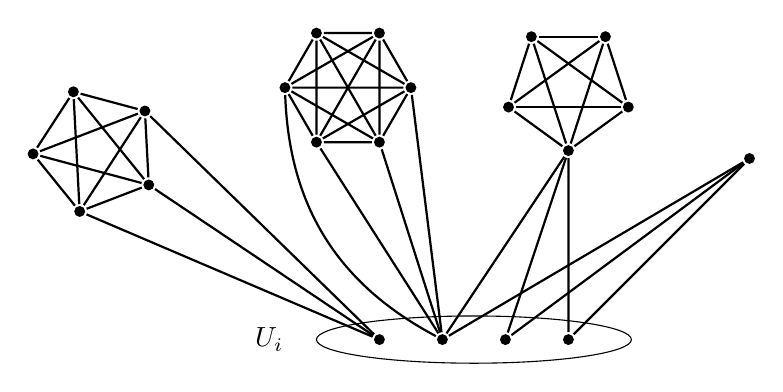
\begin{tikzpicture}[scale=1, rotate = 180]
            \GraphInit[unit=3,vstyle=Normal]
            \SetVertexNormal[Shape=circle, FillColor=black, MinSize=1pt]
            \tikzset{VertexStyle/.append style = {inner sep = 1.2, outer sep = \outers}}
            \SetVertexNoLabel
            \node at (2.6, 0) {$U_i$};
            \draw (0,0) ellipse (2cm and 0.3cm);
            \Vertex[x=-1.2, y=0]{x0}
            \Vertex[x=-0.4, y=0]{x1}
            \Vertex[x=0.4, y=0]{x2}
            \Vertex[x=1.2, y=0]{x3}
            
            \Vertex[x=-3.5, y=-2.3]{c1}
            \Edge(c1)(x0)
            \Edge(c1)(x1)
            \Edge(c1)(x2)
            
            \begin{scope}[scale=0.8, shift={(-1.5,-4)}]
                \tikzset{VertexStyle/.append style = {inner sep = 1.2pt, outer sep = \outers}}
                \begin{scope}[rotate=90]
                    \grComplete[RA=1, prefix=p]{5}
                \end{scope}
                \Edge(p0)(x0)
                \Edge(p0)(x1)
                \Edge(p0)(x2)
            \end{scope}
            
            \begin{scope}[scale=0.8, shift={(2,-4)}]
                \tikzset{VertexStyle/.append style = {inner sep = 1.2pt, outer sep = \outers}}
                \begin{scope}[rotate=60]
                    \grComplete[RA=1, prefix=t]{6}
                \end{scope}
                \Edge(x2)(t0)
                \Edge(x2)(t1)
                \Edge[style = bend left](x2)(t5)
                \Edge(x2)(t2)
            \end{scope}
            
            \begin{scope}[scale=0.8, shift={(6,-3)}]
                \tikzset{VertexStyle/.append style = {inner sep = 1.2pt, outer sep = \outers}}
                \begin{scope}[rotate=75]
                    \grComplete[RA=1, prefix=q]{5}
                \end{scope}
                \Edge(x3)(q0)
                \Edge(x3)(q1)
                \Edge(x3)(q2)
            \end{scope}
            %\draw (-4.3,-4.5) -- (-4.3, -1) -- (6.5, -1) -- (6.5,-4.5) -- (-4.3, -4.5);
            %\node at (5, -4) {$N^{2d}(U_i)$};
        \end{tikzpicture}
        \caption{The four cases that define membership in $N^{2d}(U_i)$ for $d = 2$. \label{fig:n2d}}
    \end{figure}

\begin{observation}
    For every monochromatic part $U_i$, $U_i \cup N^{2d}(U_i)$ is monochromatic.
\end{observation}

The next rules aim to increase the size of monochromatic sets.
In particular, Rule~\ref{rule:transitivity} translates the transitivity of the monochromatic property, while Rule~\ref{rule:attraction} identifies a case where merging the monochromatic sets is inevitable.

\begin{rrule}
    \label{rule:transitivity}
    If $N^{2d}(U_i) \cap N^{2d}(U_j) \neq \emptyset$, merge $U_i$ and $U_j$.
\end{rrule}

\begin{rrule}
    \label{rule:attraction}
    If there there is a set of $2d+1$ vertices $L \subseteq V(G)$ with two common neighbors $u,u'$ such that $u \in U_i$ and $u' \in U_j$, merge $U_i$ and $U_j$.
\end{rrule}

\begin{sproof}{\ref{rule:attraction}}
    Suppose that in some $d$-cut $(A, B)$, $u \in A$ and $u' \in B$, this implies that at most $d$ elements of $L$ are in $A$ and at most $d$ are in $B$, which is impossible since $|L| = 2d+1$.
\end{sproof}

We say that a cluster is \textit{small} if it has at most $2d$ vertices, and \textit{big} otherwise.
Moreover, a vertex in a cluster is \textit{ambiguous} if it has neighbors in more than one $U_i$.
A cluster is \tdef{ambiguous} if it has an ambiguous vertex, and \tdef{fixed} if it is contained in some $N^{2d}(U_i)$.

\begin{observation}
    \label{obs:fix_amb}
    If $G$ is reduced by Rule~\ref{rule:trivial}, every big cluster is ambiguous or fixed.
\end{observation}

\begin{proof}
    Since Rule~\ref{rule:trivial} cannot be applied, every cluster $C$ has either one vertex $v$ with at least $d + 1$ neighbors in $U$ or there is some vertex of a set $U_i$ with $d + 1$ neighbors in $C$.
    In the latter case, by applying the fourth case in the definition of $N^{2d}(U_i)$, we conclude that $C$ is fixed.
    In the former case, either $v$ has $d+1$ neighbors in the same $U_i$, in which case $C$ is fixed, or its neighborhood is spread across multiple monochromatic sets, and so $v$ and, consequently, $C$ are ambiguous.
\end{proof}

Our next goal is to bound the number of vertices outside of $U$.

\begin{rrule}
    \label{rule:fusion}
    If there are two clusters $C_1, C_2$ contained in some $N^{2d}(U_i)$, then add every edge between $C_1$ and $C_2$.
\end{rrule}

\begin{sproof}{\ref{rule:fusion}}
    It follows directly from the fact that $C_1 \cup C_2$ is a larger cluster, $C_1 \cup C_2 \subseteq N^{2d}(U_i)$, and that adding edges between vertices of a monochromatic set preserves the existence of a $d$-cut.
\end{sproof}

The next lemma follows from the pigeonhole principle and exhaustive application of Rule~\ref{rule:fusion}.

\begin{lemma}
    \label{lem:fixed_clusters}
    If $G$ has been reduced by Rules~\ref{rule:trivial} through~\ref{rule:fusion}, then $G$ has $\bigO{|U|}$ fixed clusters.
\end{lemma}

\begin{rrule}
    \label{rule:shrink}
    If there is some cluster $C$ with at least $2d+2$ vertices such that there is some $v \in C$ with no neighbors in $U$, remove $v$ from $G$.
\end{rrule}

\begin{sproof}{\ref{rule:shrink}}
    That $G$ has a $d$-cut if and only if $G - v$ has a $d$-cut follows directly from the hypothesis that $C$ is monochromatic in $G$ and the fact that $|C \setminus \{v\}| \geq 2d + 1$ implies that $C \setminus \{v\}$ is monochromatic in $G - v$.
\end{sproof}

By Rule~\ref{rule:shrink}, we now have the additional property that, if $C$ has more than $2d+1$ vertices, all of them have at least one neighbor in $U$. The next rule provides a uniform structure between a big cluster $C$ and the sets $U_i$ such that $C \subseteq N^{2d}(U_i)$.

\begin{rrule}
    \label{rule:normalization1}
    If a cluster $C$ has at least $2d+1$ elements and there is some $U_i$ such that $C \subseteq N^{2d}(U_i)$, remove all edges between $C$ and $U_i$, choose $u \in U_i$, $\{v_1, \dots, v_{d+1}\} \subseteq C$ and add the edges $\{uv_i\}_{i \in [d+1]}$ to $G$.
\end{rrule}

\begin{sproof}{\ref{rule:normalization1}}
    Let $G'$ be the graph obtained after the operation is applied.
    If $G$ has some $d$-cut $(A,B)$, since $U_i \cup N^{2d}(U_i)$ is monochromatic, no edge between $U_i$ and $C$ crosses the cut, so $(A,B)$ is also a $d$-cut of $G'$.
    For the converse, take a $d$-cut $(A', B')$ of $G'$.
    Since $C$ has at least $2d+1$ vertices and there is some $u \in U_i$ such that $|N(u) \cap C| = d+1$, $C \in N^{2d}(U_i)$ in $G'$.
    Therefore, no edge between $C$ and $U_i$ crosses the cut and $(A', B')$ is also a $d$-cut of $G$.
\end{sproof}

We have now effectively bounded the number of vertices in big clusters by a polynomial in $U$, as shown below.

\begin{lemma}
    \label{lem:bound1}
    If $G$ has been reduced by Rules~\ref{rule:trivial} through~\ref{rule:normalization1}, then $G$ has $\bigO{d|U|^2}$ ambiguous vertices and $\bigO{d|U|^2}$ big clusters, each with $\bigO{d|U|}$ vertices.
\end{lemma}

\begin{proof}
    To show the bound on the number of ambiguous vertices, take any two vertices $u \in U_i$, $u' \in U_j$.
    Since we have $\binom{|U|}{2}$ such pairs, if we had at least $(2d + 1)\binom{|U|}{2}$ ambiguous vertices, by the pigeonhole principle, there would certainly be $2d+1$ vertices in $V \setminus U$ that are adjacent to one pair, say $u$ and $u'$.
    This, however, contradicts the hypothesis that Rule~\ref{rule:attraction} has been applied, and so we have $\bigO{d|U|^2}$ ambiguous vertices.

    The above discussion, along with Lemma~\ref{lem:fixed_clusters} and Observation~\ref{obs:fix_amb}, imply that the number of big clusters is $\bigO{d|U|^2}$.
    For the bound on their sizes, take some cluster $C$ with at least $2d + 2$ vertices.
    Due to the application of Rule~\ref{rule:shrink}, every vertex of $C$ has at least one neighbor in $U$.
    Moreover, there is at most one $U_i$ such that $C \subseteq N^{2d}(U_i)$, otherwise we would be able to apply Rule~\ref{rule:transitivity}.

    Suppose first that there is such a set $U_i$.
    By Rule~\ref{rule:normalization1}, there is only one $u \in U_i$ that has neighbors in $C$; in particular, it has $d+1$ neighbors.
    Now, every $v \in U_j$, for every $j\neq i$, has at most $d$ neighbors in $C$, otherwise $C \subseteq N^{2d}(U_j)$ and Rule~\ref{rule:transitivity} would have been applied.
    Therefore, we conclude that $C$ has at most $(d+1) +  \sum_{v \in U \setminus U_i} |N(u) \cap C| \leq (d+1) + d|U| \in \bigO{d|U|}$ vertices.

    Finally, suppose that there is no $U_i$ such that $C \subseteq N^{2d}(U_i)$.
    A similar analysis from the previous case can be performed: every $u \in U_i$ has at most $d$ neighbors in $C$, otherwise $C \subseteq N^{2d}(U_i)$ and we conclude that $C$ has at most $\sum_{v \in U} |N(u) \cap C| \leq d|U| \in \bigO{d|U|}$ vertices.
\end{proof}


We are now left only with an unbounded number of small clusters.
A cluster $C$ is \tdef{simple} if it is not ambiguous, that is, if for each $v \in C$, $v$ has neighbors in a single $U_i$.
Otherwise, $C$ is ambiguous and, because of Lemma~\ref{lem:bound1}, there are at most $\bigO{d|U|^2}$ such clusters.
As such, for a simple cluster $C$ and a vertex $v \in C$, we denote by $U(v)$ the monochromatic set of $U$ to which $v$ is adjacent.

\begin{rrule}
    \label{rule:super_small}
    If $C$ is a simple cluster with at most $d+1$ vertices, remove $C$ from $G$.
\end{rrule}

\begin{sproof}{\ref{rule:super_small}}
    Let $G' = G - C$.
    Suppose $G$ has a $d$-cut $(A,B)$ and note that $A \nsubseteq C$ and $B \nsubseteq C$ since Rule~\ref{rule:trivial} does not apply.
    This implies that $(A \setminus C, B \setminus C)$ is a valid $d$-cut of $G'$.
    For the converse, take a $d$-cut $(A', B')$ of $G'$, define $C_A = \{v \in C \mid U(v) \subseteq A\}$, and define $C_B$ similarly; we claim that $(A' \cup C_A, B' \cup C_B)$ is a $d$-cut of $G$.
    To see that this is the case, note that each vertex of $C_A$ (resp. $C_B$) has at most $d$ edges to $C_B$ (resp. $C_A$) and, since $C$ is simple, $C_A$ (resp. $C_B$) has no other edges to $B'$ (resp. $A'$).
\end{sproof}

After applying the previous rule, every cluster $C$ not yet analyzed has size $d+2 \leq |C| \leq 2d$ which, in the case of the \pname{Matching Cut} problem, where $d=1$, is empty.
To deal with these clusters, given a $d$-cut $(A, B)$, we say that a vertex $v$ is in its \tdef{natural assignment} if $v \cup U(v)$ is in the same side of the cut; otherwise the vertex is in its \tdef{unnatural assignment}.
Similarly, a cluster is \tdef{unnaturally assigned} if it has an unnaturally assigned vertex, otherwise it is \tdef{naturally assigned}.

\begin{observation}
    \label{obs:constrained_unnatural}
    Let $\mathcal{C}$ be the set of all simple clusters with at least $d+2$ and no more than $2d$ vertices, and $(A,B)$ a partition of $V(G)$.
    If there are $d|U|+1$ edges $uv$, $v \in C \in \mathcal{C}$ and $u \in U$, such that $uv$ is crossing the partition, then $(A,B)$ is not a $d$-cut.
\end{observation}

\begin{proof}
    Since there are $d|U| + 1$ edges crossing the partition between $\mathcal{C}$ and $U$, there must be at least one $u \in U$ with $d+1$ neighbors in the other set of the partition.
\end{proof}

\begin{corollary}
    \label{cor:constrained_unnatural}
    In any $d$-cut of $G$, there are at most $d|U|$ unnaturally assigned vertices.
\end{corollary}

%\ig{HERE}

Our next lemma limits how many clusters in $\mathcal{C}$ relate in a similar way to $U$; we say that two simple clusters $C_1, C_2$ have the same \tdef{pattern} if they have the same size $s$ and there is a total ordering of $C_1$ and another of $C_2$ such that, for every $i \in [s]$, $v_i^1 \in C_1$ and $v_i^2 \in C_2$ satisfy $U(v_i^1) = U(v_i^2)$.
Essentially, clusters that have the same pattern have neighbors in exactly the same monochromatic sets of $U$ and the same multiplicity in terms of how many of their vertices are adjacent to a same monochromatic set $U_i$. Note that the actual neighborhoods in the sets $U_i$'s do not matter in order for two clusters to have the same pattern.
Figure~\ref{fig:assignment} gives an example of a maximal set of unnaturally assigned clusters; that is, any other cluster with the same pattern as the one presented must be naturally assigned, otherwise some vertex of $U$ will violate the $d$-cut property.

\begin{figure}[!htb]
        \centering
        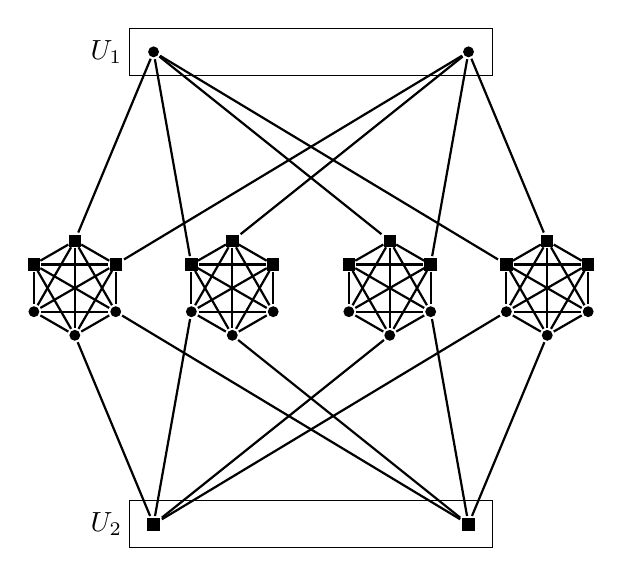
\begin{tikzpicture}[rotate = 90]
                %\draw[help lines] (-5,-5) grid (5,5);
                \GraphInit[unit=3,vstyle=Normal]
                \SetVertexNormal[Shape=circle, FillColor = black, MinSize=3pt]
                \tikzset{VertexStyle/.append style = {inner sep = \inners, outer sep = \outers}}
                \SetVertexNoLabel
                \begin{scope}[shift={(-3, 0)}]
                    \tikzset{VertexStyle/.append style = {shape = rectangle, inner sep = 2pt}}
                    \node at (0, 2.6) {$U_2$};
                    \draw (-0.3, 2.3) rectangle (0.3, -2.3);
                    \Vertex[x = 0, y = 2]{u11}
                    \Vertex[x = 0, y = -2]{u12}
                \end{scope}
                \begin{scope}[shift={(3, 0)}]
                    \node at (0, 2.6) {$U_1$};
                    \draw (-0.3, 2.3) rectangle (0.3, -2.3);
                    \Vertex[x = 0, y = 2]{u21}
                    \Vertex[x = 0, y = -2]{u22}
                \end{scope}
                
                \begin{scope}[shift={(0, 3)}]
                    \grComplete[RA=0.6, prefix=q1]{6}
                    \begin{scope}
                        \tikzset{VertexStyle/.append style = {shape = rectangle, inner sep = 2pt}}
                        \Vertex[Node]{q10}
                        \Vertex[Node]{q11}
                        \Vertex[Node]{q15}
                    \end{scope}
                    \Edge(u11)(q13)
                    \Edge(u12)(q14)
                    \Edge(u21)(q10)
                    \Edge(u22)(q15)
                \end{scope}
                
                \begin{scope}[shift={(0, 1)}]
                    \grComplete[RA=0.6, prefix=q2]{6}
                    \begin{scope}
                        \tikzset{VertexStyle/.append style = {shape = rectangle, inner sep = 2pt}}
                        \Vertex[Node]{q20}
                        \Vertex[Node]{q21}
                        \Vertex[Node]{q25}
                    \end{scope}
                    \Edge(u11)(q22)
                    \Edge(u12)(q23)
                    \Edge(u22)(q20)
                    \Edge(u21)(q21)
                \end{scope}
                
                \begin{scope}[shift={(0, -1)}]
                    \grComplete[RA=0.6, prefix=q3]{6}
                    \begin{scope}
                        \tikzset{VertexStyle/.append style = {shape = rectangle, inner sep = 2pt}}
                        \Vertex[Node]{q30}
                        \Vertex[Node]{q31}
                        \Vertex[Node]{q35}
                    \end{scope}
                    \Edge(u12)(q34)
                    \Edge(u11)(q33)
                    \Edge(u21)(q30)
                    \Edge(u22)(q35)
                \end{scope}
                
                \begin{scope}[shift={(0, -3)}]
                    \grComplete[RA=0.6, prefix=q4]{6}
                    \begin{scope}
                        \tikzset{VertexStyle/.append style = {shape = rectangle, inner sep = 2pt}}
                        \Vertex[Node]{q40}
                        \Vertex[Node]{q41}
                        \Vertex[Node]{q45}
                    \end{scope}
                    \Edge(u11)(q42)
                    \Edge(u12)(q43)
                    \Edge(u22)(q40)
                    \Edge(u21)(q41)
                \end{scope}
                
        \end{tikzpicture}
        \caption{Example of a maximal set of unassigned clusters. Square vertices would be assigned to $A$, circles to $B$ ($d=4$).\label{fig:assignment}}
    \end{figure}



\begin{lemma}
    \label{lem:patterns}
    Let $\mathcal{C}^* \subseteq \mathcal{C}$ be a subfamily of simple clusters, all with the same pattern, with $|\mathcal{C}^*| > d|U| + 1$. Let $C$ be some cluster of $\mathcal{C}^*$, and $G' = G - C$. Then
    $G$ has a $d$-cut if and only if $G'$ has a $d$-cut.
\end{lemma}

\begin{proof}
    Since by Rule~\ref{rule:trivial} no subset of a small cluster is alone in a side of a partition and, consequently, $U$ intersects both sides of the partition, if $G$ has a $d$-cut, so does $G'$.

    For the converse, let $(A', B')$ be a $d$-cut of $G'$.
    First, by Corollary~\ref{cor:constrained_unnatural}, we know that at least one of the clusters of $\mathcal{C}^* \setminus \{C\}$, say $C_{\mathsf{n}}$, is naturally assigned.
    Since all the clusters in $\mathcal{C^*}$ have the same pattern, this guarantees that \textit{any} of the vertices of a naturally assigned cluster cannot have more than $d$ neighbors in the other side of the partition.

    Let $(A,B)$ be the bipartition of $V(G)$ obtained from $(A',B')$ such that $u \in C$ is in $A$ (resp. $B$) if and only if $U(u) \subseteq A$ (resp. $U(u) \subseteq B$); that is, $C$ is naturally assigned.
    Define $C_A = C \cap A$ and $C_B = C \cap B$.
    Because $|C| = |C_{\mathsf{n}}|$ and both belong to $\mathcal{C}^*$, we know that for every $u \in C_A$, it holds that $|N(u) \cap C_B| \leq d$; moreover, note that $N(u) \cap (B \setminus C) = \emptyset$. A symmetric analysis applies to every $u \in C_B$.
    This implies that no vertex of $C$ has additional neighbors in the other side of the partition outside of its own cluster and, therefore, $(A, B)$ is a $d$-cut of $G$.
\end{proof}

The safeness of our last rule follows directly from Lemma~\ref{lem:patterns}.

\begin{rrule}
    \label{rule:pattern_removal}
    If there is some pattern such that the number of simple clusters with that pattern is at least $d|U|+2$, delete all but $d|U|+1$ of them.
\end{rrule}

\begin{lemma}
    \label{lem:bound2}
    After exhaustive application of Rules~\ref{rule:trivial} through~\ref{rule:pattern_removal}, $G$ has $\bigO{d|U|^{2d}}$ small clusters and $\bigO{d^2|U|^{2d+1}}$ vertices in these clusters.
\end{lemma}

\begin{proof}
    By Rule~\ref{rule:super_small}, no small cluster with less than $d+2$ vertices remains in $G$.
    Now, for the remaining sizes, for each $d+2 \leq s \leq 2d$, and each pattern of size $s$, by Rule~\ref{rule:pattern_removal} we know that the number of clusters with $s$ vertices that have the same pattern is at most $d|U| + 1$.
    Since we have at most $|U|$ possibilities for each of the $s$ vertices of a cluster, we end up with $\bigO{|U|^{s}}$ possible patterns for clusters of size $s$.
    Summing all of them up, we get that we have $\bigO{|U|^{2d}}$ patterns in total, and since each one has at most $d|U| + 1$ clusters of size at most $2d$, we get that we have at most $\bigO{d^2|U|^{2d+1}}$ vertices in those clusters.
\end{proof}

The exhaustive application of all the above rules and their accompanying lemmas are enough to show that indeed, there is a polynomial kernel for \pname{$d$-Cut} when parameterized by distance to cluster.


\begin{theorem}
    When parameterized by distance to cluster $\dc(G)$, \pname{$d$-Cut} admits a polynomial kernel with $\bigO{d^2\dc(G)^{2d+1}}$ vertices that can be computed in $\bigO{d^4\dc(G)^{2d+1}(n+m)}$ time.
\end{theorem}

\begin{proof}
    The algorithm begins by finding a set $U$ such that $G - U$ is a cluster graph.
    Note that $|U| \leq 3\dc(G)$ since a graph is a cluster graph if and only if it has no induced path on three vertices: while there is some $P_3$ in $G$, we know that at least one its vertices must be removed, but since we don't know which one, we remove all three; thus, $U$ can be found in $\bigO{\dc(G)(n + m)}$ time.
    After the exhaustive application of Rules~\ref{rule:trivial} through~\ref{rule:pattern_removal}, by Lemma~\ref{lem:bound1}, $V(G) \setminus U$ has at most $\bigO{d^2\dc(G)^3}$ vertices in clusters of size at least $2d+1$.
    By Rule~\ref{rule:super_small}, $G$ has no simple cluster of size at most $d+1$.
    Ambiguous clusters of size at most $2d$, again by Lemma~\ref{lem:bound1}, also comprise only $\bigO{d^2\dc(G)^2}$ vertices of $G$.
    Finally, for simple clusters of size between $d+2$ and $2d$, Lemmas~\ref{lem:patterns} and~\ref{lem:bound2} guarantee that there are $\bigO{d^2\dc(G)^{2d+1}}$ vertices in small clusters and, consequently, this many vertices in $G$.

    As to the running time, first, computing and maintaining $N^{2d}(U_i)$ takes $\bigO{d\dc(G)n}$ time.
    Rule~\ref{rule:trivial} is applied only at the beginning of the kernelization, and runs in $\bigO{2^{2d}d(n + m)}$ time.
    Rules~\ref{rule:transitivity} and~\ref{rule:attraction} can both be verified in $\bigO{d\dc(G)^2(n + m)}$ time, since we are just updating $N^{2d}(U_i)$ and performing merge operations.
    Both are performed only $\bigO{\dc(G)^2}$ times, because we only have this many pairs of monochromatic parts.
    The straightforward application of Rule~\ref{rule:fusion} would yield a running time of $\bigO{n^2}$. However, we can ignore edges that are interior to clusters and only maintain which vertices belong together; this effectively allows us to perform this rule in $\bigO{n}$ time, which, along with its $\bigO{n}$ possible applications, yields a total running time of $\bigO{n^2}$ for this rule.
    Rule~\ref{rule:shrink} is directly applied in $\bigO{n}$ time; indeed, all of its applications can be performed in a single pass.
    Rule~\ref{rule:normalization1} is also easily applied in $\bigO{n + m}$ time. Moreover, it is only applied $\bigO{\dc(G)}$ times, since, by Lemma~\ref{lem:bound1}, the number of fixed clusters is linear in $\dc(G)$; furthermore, we may be able to reapply Rule~\ref{rule:normalization1} directly to the resulting cluster, at no additional complexity cost.
    The analysis for Rule~\ref{rule:super_small} follows the same argument as for Rule~\ref{rule:shrink}.
    Finally, Rule~\ref{rule:pattern_removal} is the bottleneck of our kernel, since it must check each of the possible $\bigO{\dc(G)^{2d}}$ patterns, spending $\bigO{n}$ time for each of them.
    Each pattern is only inspected once because the number of clusters in a pattern can no longer achieve the necessary bound for the rule to be applied once the excessive clusters are removed.
\end{proof}

In the next theorem we provide an \FPT algorithm for \textsc{$d$-Cut} parameterized by the distance to cluster, running in time $\bigO{4^d(d+1)^{\dc(G)}2^{\dc(G)}\dc(G)n^2}$. Our algorithm is based on dynamic programming, and is considerably simpler than the one given by Komusiewicz  et al.~\cite{matching_cut_ipec} for $d=1$, which applies four reduction rules and an equivalent formulation as a 2-\textsc{SAT} formula. However, for $d=1$ our algorithm is slower, namely $\bigOs{4^{\dc( G )}}$ compared to  $\bigOs{2^{\dc( G )}}$.


%and explain the main differences with respect the one in~\cite{matching_cut_ipec}}

Observe that minimum distance to cluster
sets and minimum distance to co-cluster sets can be computed in $1.92^{\dc( G )} \cdot \bigO{ n^2 }$
time and $1.92^{\dcc( G )} \cdot \bigO{n^2 }$ time, respectively~\cite{branching-cluster}. Thus, in Theorems~\ref{thm:fpt_cluster} and~\ref{thm:fpt_cocluster} we can safely assume that we have these sets at hand.


\begin{theorem}
    \label{thm:fpt_cluster}
    For every integer $d \geq 1$, there is an algorithm that solves \pname{$d$-Cut} in time $\bigO{4^d(d+1)^{\dc(G)}2^{\dc(G)}\dc(G)n^2}$.
\end{theorem}

\begin{proof}
    Let $U$ be a set such that $G - U$ is a cluster graph, $\mathcal{Q} = \{Q_1, \dots, Q_p\}$ be the family of clusters of $G - U$ and $\mathcal{Q}_i = \bigcup_{i \leq j \leq p} Q_j$.
    Essentially, the following dynamic programming algorithm attempts to extend a given partition of $U$ in all possible ways by partitioning clusters, one at a time, while only keeping track of the degrees of vertices that belong to $U$.
    Recall that we do not need to keep track of the degrees of the cluster vertices precisely because $G - U$ has no edge between clusters.

    Formally, given a partition $U = A  \dcup B$, our table is a mapping $f : [p] \times \mathbb{Z}^{|A|} \times \mathbb{Z}^{|B|} \rightarrow \{0, 1\}$.
    Each entry is indexed by $(i, \bmd_A, \bmd_B)$, where $i \in [p]$, $\bmd_A$ is a $|A|$-dimensional vector with the $j$-th coordinate begin denoted by $\bmd_A[j]$; $\bmd_B$ is defined analogously.
    Our goal is to have $f(i, \bmd_A, \bmd_B) = 1$ if and only if there is a partition $(X, Y)$ of $U \cup \mathcal{Q}_i$ where $A \subseteq X$, $B \subseteq Y$ and $v_j \in A$ ($u_{\ell} \in B$) has at most $\bmd_A[j]$ ($\bmd_B[\ell]$) neighbors in $\mathcal{Q}_i$.

    We denote by $P_d(i, \bmd_A, \bmd_B)$ the set of all partitions $L  \dcup R = Q_i$ such that every vertex $v \in L$ has $d_{B \cup R}(v) \leq d$, every $u \in R$ has $d_{A \cup L}(u) \leq d$, every $v_j \in A$, $d_R(v_j) \leq \bmd_A[j]$ and every $u_{\ell} \in B$, $d_L(u_{\ell}) \leq \bmd_B[\ell]$; note that, due to this definition, $(L, R) \neq (R, L)$.
    In the following equations, which give the computations required to build our table, $\bmd_A(R)$ and $\bmd_B(L)$ are the updated values of the vertices of $A$ and $B$ after $R$ is added to $Y$ and $L$ to $X$, respectively.
    \begin{align}
        f(i, \bmd_A, \bmd_B) &= 0 \bigvee_{(L, R) \in P_d(i, \bmd_A, \bmd_B)} f(i+1,\bmd_A(R), \bmd_B(L))\label{eq:trans_dc}\\
        f(p, \bmd_A, \bmd_B) &= 1, \text{if and only if $P_d(i, \bmd_A, \bmd_B) \neq \emptyset$.}\label{eq:stop_dc}
    \end{align}

    We proceed to show the correctness of the above by induction.
    For the base case, i.e., when $|\mathcal{Q}| = p = 1$, we have that for $v_j \in A$ ($u_l \in B$),  $\bmd_A[j] = d - d_B(v_j)$ ($\bmd_B[j] = d - d_A(u_l)$) and a partition of $V(G)$ exists if and only if there is some partition $(L, R) \in P_d(1, \bmd_A, \bmd_B)$, where.
    This case is covered by equation~(\ref{eq:stop_dc}).

    So let $p > 1$ and $(i, \bmd_A, \bmd_B)$ be an entry of our table.
    First, if $|Q_i| \geq 2d+1$, $Q_i$ is monochromatic, which implies that $|P_d(i, \bmd_A, \bmd_B)| \leq 2$.
    Therefore, we may assume that, $|P_d(i, \bmd_A, \bmd_B)| \leq 2^{2d}$.
    $P_d(i, \bmd_A, \bmd_B) = \emptyset$ implies that any partition $(L, R)$ of $Q_i$ causes a vertex in $L$ ($R$) to have more than $d$ neighbors in $B \cup R$ ($A \cup L$), which is easily checked for in $\bigO{n|U|}$-time, or some vertex $v_j \in A$ ($u_l \in B$) has $d_{Y \cup R}(v_j) > \bmd_A[j]$ ($d_{X \cup L}(u_l) > \bmd_B[l]$).
    Either way, we have that no matter how we partition $\mathcal{Q}_i$, the available degree of some vertex is not enough, equation~(\ref{eq:trans_dc}) yields the correct answer.

    However, if $P_d(i, \bmd_A, \bmd_B) \neq \emptyset$, the subgraph induced by $U \cup \mathcal{Q}_i$ has a $d$-cut separating $A$ and $B$ and respecting the limits of $\bmd_A$ and $\bmd_B$ if and only if there is some $(L, R) \in P_d(i, \bmd_A, \bmd_B)$ such that $U \cup \mathcal{Q}_{i+1}$ has a $d$-cut and each vertex of $A$ ($B$) has the size of its neighborhood in $\mathcal{Q}_{i+1}$ bounded by the respective coordinate of $\bmd_A(R)$ ($\bmd_B(L)$).
    By the inductive hypothesis, there is such a partition of $\mathcal{Q}_{i+1}$ if and only if $f(i+1, \bmd_A(R), \bmd_B(L)) = 1$, concluding the proof of correctness.
    Clearly, there is a $d$-cut separating $A$ and $B$ if $f(1, \bmd_A, \bmd_B) = 1$ where for every $v_j \in A$ ($u_l \in B$),  $\bmd_A[j] = d - d_B(v_j)$ ($\bmd_B[j] = d - \dgr_A(u_{\ell})$).

    The complexity analysis is straightforward.
    Recalling that $|P_d(i, \bmd_A, \bmd_B)| \leq 2^{2d}$, we have that each $f(i, \bmd_A, \bmd_B)$ can be computed in time $\bigO{4^d|U|n}$ and, since we have $\bigO{(d+1)^{|A| + |B|}p} \in \bigO{(d+1)^{|U|}p}$, given a partition $(A, B)$ of $U$, we can decide if there is $d$-cut separating $A$ and $B$ in $\bigO{4^d(d+1)^{|U|}|U|n^2}$-time.
    To solve \pname{$d$-Cut} itself, we guess all $2^{|U|}$ partitions of $U$ and, since $|U| \in \bigO{\dc(G)}$, we obtain a total running time of $\bigO{4^d(d+1)^{\dc(G)}2^{\dc(G)}\dc(G)n^2}$.
\end{proof}

\subsection{Distance to co-cluster}
\label{sec:cocluster}

A graph is a \emph{co-cluster} graph if only if its the complement of a cluster graph; that is, if it is a complete multipartite graph.
Our next theorem complements the results of our previous section and shall help establish the membership  in $\FPT$ of \pname{$d$-Cut} parameterized by the vertex cover number.

\begin{theorem}
    \label{thm:fpt_cocluster}
    For every integer $d \geq 1$, there is an algorithm solving \pname{$d$-Cut} in time $\bigO{32^d2^{\dcc(G)}(d+1)^{\dcc(G)+d}(\dcc(G)+d)n^2}$.
\end{theorem}

\begin{proof}
    Let $U \subseteq V(G)$ be a set of $\bigO{\dcc(G)}$ vertices such that $G - U$ is a co-cluster graph with color classes $\varphi = \{F_1, \dots, F_t\}$.
    Define $\mathcal{F} = \bigcup_{i \in [t]} F_i$ and suppose we are given a $d$-cut $(A,B)$ of $G[U]$.
    First, note that if $t \geq 2d+1$, we have that some of the vertices of $\mathcal{F}$ form a clique of size $2d+1$, which is a monochromatic set; furthermore, every vertex $v \in \mathcal{F}$ but not in $Q$ has at least $d+1$ neighbors in $Q$.
    This implies that $Q \cup \{v\}$ is monochromatic and, thus, $\mathcal{F}$ is a monochromatic set.
    Checking if either $(A \cup \mathcal{F}, B)$ or $(A, B \cup \mathcal{F})$ is a $d$-cut can be done in $\bigO{n^2}$ time.

    If the above does not apply, we have that $t \leq 2d$.
    \begin{itemize}
        \item Case 1: If $|\mathcal{F}| \leq 4d$ we can just try to extend $(A,B)$ with each of the $2^{|\mathcal{F}|}$ bipartitions of $\mathcal{F}$ in $\bigO{16^dn^2}$ time.
    \end{itemize}

    So now, let $\varphi_1 \dcup \varphi_2 = \varphi$ be a bipartition of the color classes, $\mathcal{F}_i = \{v \in F_j \mid F_j \in \varphi_i\}$, and, for simplicity, suppose that $|\mathcal{F}_1|~\leq~|\mathcal{F}_2|$.

    \begin{itemize}
        \item Case 2: If $|\mathcal{F}_1| \geq d+1$ and $|\mathcal{F}_2| \geq 2d+1$, we know that there is a set $Q \subseteq \mathcal{F}$ forming a (not necessarily induced) complete bipartite subgraph $K_{d+1, 2d+1}$, which is a monochromatic set.
        Again, any $v \notin Q$ has at least $d_Q(v) \geq d+1$, from which we conclude that $Q \cup \{v\}$ is also monochromatic, implying that $\mathcal{F}$ is monochromatic.
    \end{itemize}


    If Case 2 is not applicable, either $|\mathcal{F}_1| \leq d$ and $|\mathcal{F}_2| \geq 2d+1$, or $|\mathcal{F}_2| \leq 2d$.
    For the latter, note that this implies $|\mathcal{F}| \leq 4d$, which would have been solved by Case 1.
    For the former, two cases remain:

    \begin{itemize}
        \item Case 3: Every $F_i \in \varphi_2$ has $|F_i| \leq 2d$. This implies that every $F \in \varphi$ has size bounded by $2d$ and that $|\mathcal{F}| \leq 4d^2$; we can simply try to extend $(A, B)$ with each of the $\bigO{2^{d^2}}$ partitions of $\mathcal{F}$, which can be done in $\bigO{2^{d^2}n^2}$ time.

        \item Case 4: There is some $F_i \in \varphi_2$ with $|F_i| \geq 2d + 1$.
        Its existence implies that $|\mathcal{F}| - |F_i| \leq d$, otherwise we would have concluded that $\mathcal{F}$ is a monochromatic set.
        Since $\mathcal{F} \setminus F_i$ has at most $d$ vertices, the set of its bipartitions has size bounded by $2^d$.
        So, given a bipartition $\mathcal{F}_A \dcup \mathcal{F}_B = \mathcal{F} \setminus F$, we define $A' := A \cup \mathcal{F}_A$ and $B' := B \cup \mathcal{F}_B$.
        Finally, note that $G \setminus (A' \cup B')$ is a cluster graph where every cluster is a single vertex; that is, $\dc(G) \leq \dcc(G) + d$.
        In this case, we can apply Theorem~\ref{thm:fpt_cluster}, and obtain the running time of $\bigO{4^d(d+1)^{\dcc(G)+d}(\dcc(G)+d)n^2}$; we omit the term $2^{\dcc(G) + d}$ since we already have an initial partial $d$-cut $(A', B')$.
    \end{itemize}

    For the total complexity of the algorithm, we begin by guessing the initial partition of $U$ into $(A,B)$, spending $\bigO{n^2}$ time for each of the $\bigO{2^{\dcc(G)}}$ possible bipartitions.
    If $t \geq 2d+1$ we give the answer in $\bigO{n^2}$ time.
    Otherwise, $t \leq 2d$.
    If $|\mathcal{F}| \leq 4d$, then we spend $\bigO{16^dn^2}$ time to test all partitions of $\mathcal{F}$ and return the answer.
    Else, for each of the $\bigO{4^d}$ partitions of $\varphi$, if one of them has a part with $d+1$ vertices and the other part has $2d+1$ vertices, we respond in $\bigO{n^2}$ time.
    Finally, for the last two cases, we either need $\bigO{2^{d^2}n^2}$ time, or $\bigO{8^d(d+1)^{\dcc(G)+d}(\dcc(G)+d)n^2}$.
    This yields a final complexity of $\bigO{32^d2^{\dcc(G)}(d+1)^{\dcc(G)+d}(\dcc(G)+d)n^2}$.
\end{proof}

Using Theorems~\ref{thm:fpt_cluster},~\ref{thm:fpt_cocluster}, and the relation $\tau(G) \geq \max\{\dc(G), \dcc(G)\}$~\cite{matching_cut_ipec}, we obtain fixed-parameter tractability for the vertex cover number $\tau(G)$.

\begin{corollary}
    For every $d \geq 1$, \pname{$d$-Cut} parameterized by the vertex cover number is in $\FPT$.
\end{corollary}

\section{Concluding remarks}


We presented a series of algorithms and complexity results; many questions, however, remain open.
For instance, all of our algorithms have an exponential dependency on $d$ on their running times.
While we believe that such a dependency is an intrinsic property of \pname{$d$-cut}, we have no proof for this claim. Similarly, the existence of a \textit{uniform} polynomial kernel parameterized by the distance to cluster, i.e., a kernel whose degree does not depend on $d$, remains an interesting open question.

Also in terms of running time, we expect the constants in the base of the exact exponential algorithm to be improvable. However, exploring small structures that yield non-marginal gains as branching rules, as done by Komusiewicz et al.~\cite{matching_cut_ipec} for $d=1$ does not seem a viable approach, as the number of such structures appears to rapidly grow along with $d$.

%\ig{uniform kernel?}


The distance to cluster kernel is hindered by the existence of clusters of size between $d+2$ and $2d$, an obstacle that is not present in the \pname{Matching Cut} problem.
Aside from the extremal argument presented, we know of no way of dealing with them.
We conjecture that it should be possible to reduce the total kernel size from $\bigO{d^2\dc(G)^{2d+1}}$ to $\bigO{d^2\dc(G)^{2d}}$, matching the size of the smallest known kernel for \pname{Matching Cut}~\cite{matching_cut_ipec}.

We also leave open to close the gap between the known polynomial and $\NP$-hard cases in terms of maximum degree.
We showed that, if $\Delta(G) \leq d+2$ the problem is easily solvable in polynomial time, while for graphs with $\Delta(G) \geq 2d+2$, it is $\NP$-hard.
But what about the gap $d+3 \leq \Delta(G) \leq 2d+1$?
After much effort, we were unable to settle any of these cases.
In particular, we are very interested in \pname{2-Cut},  which has a single open case, namely when $\Delta(G) = 5$.
After some weeks of computation, we found no graph with more than 18 vertices and maximum degree five that had no $2$-cut, in agreement with the computational findings of Ban and Linial~\cite{internal_partition_regular6}.
Interestingly, all graphs on 18 vertices without a $2$-cut are either 5-regular or have a single pair of vertices of degree 4, which are actually adjacent.
In both cases, the graph is maximal in the sense that we cannot add edges to it while maintaining the degree constraints.
We recall the initial discussion about the \pname{Internal Partition} problem; closing the gap between the known cases for \textsc{$d$-Cut} would yield significant advancements on the former problem.

Finally, the smallest $d$ for which $G$ admits a $d$-cut may be an interesting additional parameter to be considered when more traditional parameters, such as treewidth, fail to provide $\FPT$ algorithms by themselves.
Unfortunately, by Theorem~\ref{thm:regular_nph}, computing this parameter is not even in $\XP$, but, as we have shown, it can be computed in $\FPT$ time under many different parameterizations. 


\chapter{On the intersection graph of maximal stars}
\label{ch:star_graph}


Intersection graphs form the basis for much of the theory on graph classes.
For instance, the class of chordal graphs, which is one of the most fundamental and broadly studied classes~\cite{classes_survey}, can be defined as precisely the family of intersection graphs of all subtrees of some tree.
Interval graphs, in turn, are defined as the family of intersection graphs of subpaths of some path.
Line graphs are the intersection graphs of the edges of some graph.
Unlike chordal graphs, there are known characterizations for line graphs that make use of a finite family of forbidden induced subgraphs~\citep{line_nich}.
Moreover, line graphs were one of the first classes to be characterized in terms of edge clique covers that satisfy some properties pertinent to the intersection definition; results of this form are known as \tdef{Krausz-type characterizations}.

All of the aforementioned classes are easily recognizable in polynomial time~\cite{classes_survey,line_naor}.
The complexity of recognizing clique graphs -- the intersection graphs of the maximal cliques of some graph -- was an open problem for decades, with a very complicated argument, due to~\cite{clique_recognition}, showing that the problem is $\NPc$.
Many other aspects of clique graphs have been investigated in the literature.
Such is the case for, clique-critical graphs -- graphs whose clique graph is different from the clique graph of all of its proper induced subgraphs.
This graph class has its own characterizations~\cite{clique_critical_toft} and bounds~\cite{clique_critical_alcon} which were central in the proof of the complexity of the clique graph recognition problem.
Another common line of investigation on intersection graphs is the study of iterated intersection graphs, i.e., of the behavior of a graph that undergoes the operation multiple consecutive times.
Results of this flavor usually come in the form of convergence, divergence, and periodicity theorems, relating properties of the input graph to the behavior of the limit graph (after applying the operator an infinite number of times).
A closely related intersection class to star graphs is that of biclique graphs -- the intersection graph of the maximal induced complete bipartite graphs of a graph.
The introductory paper by~\cite{biclique_graph} gives a Krausz-type characterization of the class and some properties of its members; these results, however, are not very useful from the algorithmic point of view, and appear to not yield many insights on the recognition problem.

Star graphs and biclique graphs coincide for $C_4$-free graphs and our initial hope was that results on the former would yield advancements on the latter.
While we were unable to achieve our original goal, we present an introductory study of the intersection graphs of maximal stars, providing answers to some difficulties we encountered when working with the class.
After some standard definitions of the theory of intersection graphs, we begin the discussion with a bound on the number of vertices of star-critical graphs by a quadratic function of the size of its set of maximal stars.
Afterwards, we give a Krausz-type characterization, which, when combined to the previous result, shows that the recognition problem belongs to \NP.
We then shift the focus, to properties of star graphs.
In particular, we show that they are biconnected, that every edge belongs to at least one triangle, we characterize the structures that the pre-image must have in order to generate degree two vertices, and bound the diameter of the star graph with respect to the diameter of its pre-image is given.
Finally, we give a monotonicity theorem, which is used to generate all star graphs on no more than eight vertices and prove that the class of star graphs and square graphs are not properly contained in each other.


\section{Intersection graphs}
\label{sec:intersections}

Some interesting intersection graphs are usually defined in terms of the intersection of structures of other graphs. For instance, \tdef{line graphs} are precisely the graphs that are the intersection graphs of the edges of a graph; \tdef{clique graphs} are the intersection graphs of the maximal induced cliques of a graph.
Both of these classes, however have nice characterizations in terms of edge clique covers, which are commonly called \tdef{Krausz-type characterizations}.

\begin{class_definition*}[Line Graph]
    $G$ is a line graph if and only if there is an edge clique cover $\mathcal{Q}$ of $G$ such that both conditions hold:
        \begin{itemize}
            \item[(i)] Every vertex of $G$ appears in exactly two members of $\mathcal{Q}$;
            \item[(ii)] Every edge of $G$ is in only one member of $\mathcal{Q}$.
        \end{itemize}
\end{class_definition*}

\begin{class_definition*}[Clique Graph]
    $G$ is a clique graph if and only if it there is an edge clique cover of $G$ satisfying the Helly property.
\end{class_definition*}

\begin{figure}[!htb]
    \centering
        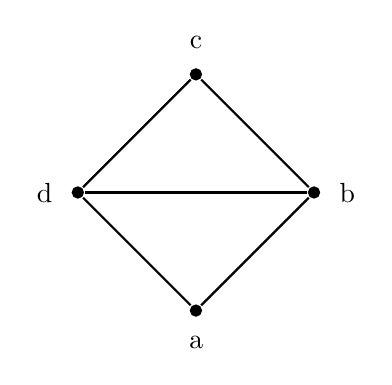
\begin{tikzpicture}
            \begin{scope}[rotate=-90,scale=0.5]
                \def\x{-2}
                \GraphInit[vstyle=Normal]
                \SetVertexNormal[Shape=circle, FillColor=black, LineWidth=1pt,MinSize=2pt,]
                \tikzset{VertexStyle/.append style = {inner sep = \inners, outer sep = \outers}}
                \Vertices[Lpos=270,Ldist=3pt,LabelOut=TRUE,unit=3]{circle}{a,b,c,d}
                \Edge(a)(b)
                \Edge(a)(d)
                \Edge(c)(b)
                \Edge(d)(b)
                \Edge(c)(d)
            \end{scope}
        \end{tikzpicture}
    \hfill
        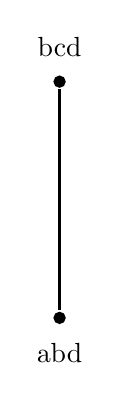
\begin{tikzpicture}
            \begin{scope}[rotate=-90,scale=0.5]
                \def\x{-2}
                \GraphInit[vstyle=Normal]
                \SetVertexNormal[Shape=circle, FillColor=black, LineWidth=1pt,MinSize=2pt,]
            \tikzset{VertexStyle/.append style = {inner sep = \inners, outer sep = \outers}}
                \Vertices[Lpos=270,Ldist=3pt,LabelOut=TRUE,unit=3]{circle}{abd,bcd}
                \Edge(abd)(bcd)
            \end{scope}
        \end{tikzpicture}
    \hfill
        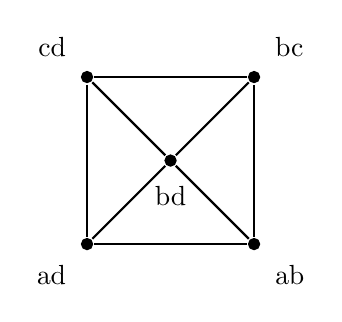
\begin{tikzpicture}
            \begin{scope}[rotate=315,scale=0.5]
                \def\x{-2}
                \GraphInit[vstyle=Normal]
                \SetVertexNormal[Shape=circle, FillColor=black, LineWidth=1pt,MinSize=2pt,]
            \tikzset{VertexStyle/.append style = {inner sep = \inners, outer sep = \outers}}
                \Vertices[Lpos=315,Ldist=3pt,LabelOut=TRUE,unit=3]{circle}{ab,bc,cd,ad}
                \Vertex[Lpos=270,Ldist=3pt,LabelOut=TRUE,unit=3,x=0,y=0]{bd}
                \Edge(ab)(bc)
                \Edge(ab)(ad)
                \Edge(bc)(cd)
                \Edge(cd)(ad)
                \Edge(bd)(ab)
                \Edge(bd)(ad)
                \Edge(bd)(cd)
                \Edge(bd)(bc)
            \end{scope}
        \end{tikzpicture}
    \hfill
        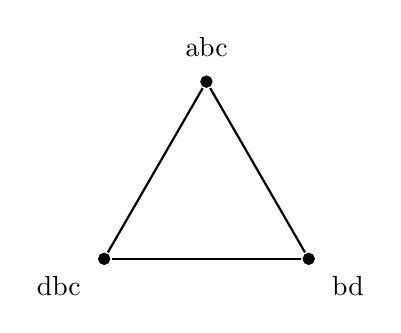
\begin{tikzpicture}
            \begin{scope}[rotate=90,scale=0.5]
                \GraphInit[vstyle=Normal]
                \SetVertexNormal[Shape=circle, FillColor=black, LineWidth=1pt,MinSize=2pt,]
            \tikzset{VertexStyle/.append style = {inner sep = \inners, outer sep = \outers}}
                \Vertices[Lpos=90,Ldist=3pt,LabelOut=TRUE,unit=3]{circle}{abc,dbc,bd}
                \Edges(abc,dbc,bd,abc)
            \end{scope}
        \end{tikzpicture}
    \hfill
    \caption{A graph, its clique graph, its line graph, and its star graph}
    %  Some graph
    \label{fig:my_label}
\end{figure}

The recognition of line graphs is known to be efficient~\citep{line_dynamic,line_nich,line_naor}.
For clique graphs, however, the situation was not so simple, and the complexity of clique graph recognition was left open for several years, finally being proven to be $\NPc$ by~\cite{clique_recognition} with a quite complicated argument.

Aside from the complexity point of view, many different properties of intersection graphs have been investigated in the literature.
For instance, clique-critical graphs -- graphs whose clique graph is different from the clique graph of all of its proper induced subgraphs -- have different characterizations~\citep{clique_critical_toft} and bounds~\citep{clique_critical_alcon} which were crucial in the proof of the complexity of the recognition problem.
Another common line of investigation on intersection graphs is the behaviour of iterated applications of the operators.
For instance, \cite{clique_iterated}, and \cite{clique_divergent} study iterated applications of the clique operator.
Biclique graphs -- the intersection graph of the maximal induced complete bipartite graphs of a graph -- were first characterized and studied by \cite{biclique_graph}.
Their results, however, are not very useful from the algorithmic point of view, and appear to not yield many insights on the recognition problem.
Nevertheless, they study the behavior of biclique graphs, showing that every edge is contained either in a diamond or a 3-fan and specialize their general characterization for biclique graphs of bipartite graphs.
As was done for clique graphs, the iterated biclique operator has also been studied by Groshaus et al. in multiple papers~\citep{biclique_iterated, almost_all_biclique}, with results ranging from characterizations of divergence, divergence type verification algorithms, and other structural results.

For other classical results in the area we point to~\citep{intersection_graphs}, from where most of the given definitions come from.

\subsection{Maximal stars}
\label{sec:maximal_stars}

Regarding stars, previous work handled the intersection graphs of (not necessarily maximal) substars of a tree~\citep{substar_graph} and of a star~\citep{starlike_graph}.
For the first, a minimal infinite family of forbidden induced subgraphs was given, while, for the latter, a series of characterizations were shown (including a finite family of forbidden induced subgraphs).
Stars are a particular case of bicliques, and both the biclique graph and star graph coincide for $C_4$-free graphs.
In fact, this relationship was successfully applied to determine the complexity of biclique coloring~\citep{biclique_coloring_complexity}, as discussed in Chapter~\ref{ch:coloring}.
To the best of our knowledge, these are the main topics discussed in the literature that involve maximal stars in some way.
The central object of study in this chapter is the intersection graph of maximal stars, which we formally define in Definition~\ref{def:star_graph}.


\begin{definition}\label{def:star_graph}
    Let $\mathcal{G}$ be the set of all finite graphs and $\str(H)$ be the set of all induced maximal stars of a graph $H$. The \tdef{star operator} is the function $\K{S} : \mathcal{G} \mapsto \mathcal{G}$ such that, $\K{S}(H) = \Omega(\str(H))$.
    If $G = \K{S}(H)$, we say that $H$ is a \tdef{pre-image} of $G$ and that $G$ is the \tdef{star graph} of $H$.
    The \textit{iterated star operator} $\K{S}^i$ is defined as $\K{S}^1(H) = \K{S}(H)$ and $\K{S}^i(H) = \K{S}(\K{S}^{i-1}(H))$.
\end{definition}

When detailing which vertices belong to a star $s$, we shall describe it by $s = \{v_1\}\{v_2, \dots, v_{p+1}\}$, with $v_1$ being its center, denoted by $c(s) = v_1$, and the other $p$ vertices its leaves.
Unless noted, $G$ will be our star graph and $H$ the pre-image of $G$. %
%The family of all maximal stars of $G$ is denoted by $\str(G)$.
By Definition~\ref{def:star_graph}, two stars $s_a,s_b$ intersect if they share at least one vertex, with the possible cases being: (i) the centers of $s_a$ and $s_b$ coincide; (ii) the center of $s_a$ is a leaf of $s_b$; or (iii) $s_a$ and $s_b$ share at least one leaf.
Note that conditions (i) and (iii) may be simultaneously satisfied.
For an example of the intersection possibilities, please refer to Figure~\ref{fig:intersection_example}.


\begin{figure}[!tb]
    \centering
        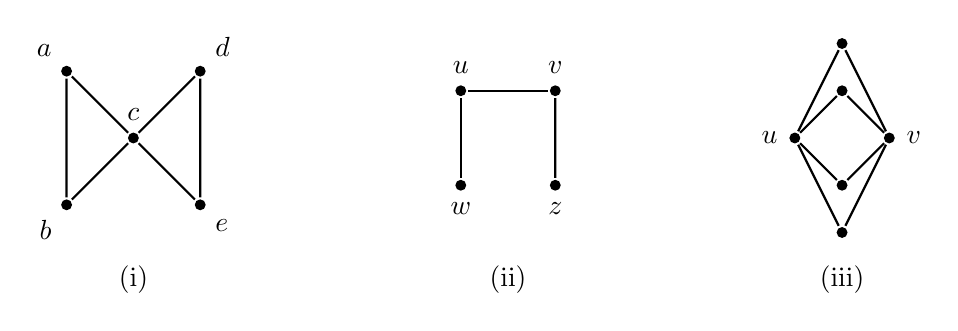
\begin{tikzpicture}[scale=1.2]
            \GraphInit[unit=3,vstyle=Normal]
            \SetVertexNormal[Shape=circle, FillColor = black, MinSize=3pt]
            \tikzset{VertexStyle/.append style = {inner sep = \inners,outer sep = \outers}}
            \SetVertexLabelOut
            \begin{scope}[xshift=-3.5cm]
                \Vertex[x=0,y=0, Math, Lpos=90]{c}
                
                \Vertex[a=135, d=1, Math, Lpos=135]{a}
                \Vertex[a=225, d=1, Math, Lpos=225]{b}
                
                \Vertex[a=315, d=1, Math, Lpos=315]{e}
                \Vertex[a=45, d=1, Math, Lpos=45]{d}
                \node at (0,-1.5) {(i)};
                \Edges(b,c,d,e,c,a,b)
            \end{scope}
            \begin{scope}[xshift=-1, yshift=0.5cm]
                \Vertex[x=0,y=0, Math, Lpos=90, L={u}]{up}
                \Vertex[x=1,y=0, Math, Lpos=90, L={v}]{vp}
                
                \Vertex[x=0,y=-1, Math, Lpos=270]{w}
                \Vertex[x=1,y=-1, Math, Lpos=270]{z}
                \node at (0.5,-2) {(ii)};
                \Edges(w,up,vp,z)
            \end{scope}
            \begin{scope}[xshift=3.5cm]
                \Vertex[x=0,y=0, Math, Lpos=180]{u}
                \Vertex[x=1,y=0, Math, Lpos=0]{v}
                
                \Vertex[x=0.5,y=0.5, Math, NoLabel]{x_1}
                \Vertex[x=0.5,y=1, Math, NoLabel]{x_2}
                \Vertex[x=0.5,y=-0.5, Math, NoLabel]{x_3}
                \Vertex[x=0.5,y=-1, Math, NoLabel]{x_4}
                
                \node at (0.5,-1.5) {(iii)};
                \Edges(u,x_1,v,x_2,u,x_3,v,x_4,u)
            \end{scope}
        \end{tikzpicture}
        \caption{(i) The stars $\{c\}\{a,e\}$ and $\{c\}\{b,d\}$ intersect only at their center; (ii) center of $\{u\}\{w,v\}$ is a leaf of star $\{v\}\{u,z\}$; (iii) the star centered at $u$ intersects the star centered at $v$ only at their leaves.\label{fig:intersection_example}}
\end{figure}


We say that star $s_a$ \textit{absorbs} star $s_b$ if, by removing one leaf of $s_b$, it becomes a substar of $s_a$.
A vertex $v$ is said to be \tdef{star-critical} if its removal changes the resulting star graph; that is, the star graph of $H$ and the star graph of $H \setminus \{v\}$ are not isomorphic.
Similarly to clique-critical graphs~\cite{clique_critical_toft,clique_critical_alcon}, a graph is \textit{star-critical} if all of its vertices are star-critical.
It is not hard to see that the only vertices which may be non-star-critical are simplicial vertices; for example, if there is a class of false twin simplicial vertices, all but one of them are certainly non-star-critical.

When detailing which vertices belong to a star, we shall describe it by $\{v_1\}\{v_2, \dots, v_{n+1}\}$, with $v_1$ being its center and the other $n$ vertices its leaves.
If the star is a single edge, choose one of the vertices to be the center and the other to be the leaf arbitrarily.
Unless noted, $G$ will be our star graph and $H$ the pre-image of $G$.
The family of all maximal stars of $G$ is denoted by $\str(G)$.
For the entirety of this work, we assume that all of our graphs are connected.



\begin{figure}[!htb]
	\centering
	
	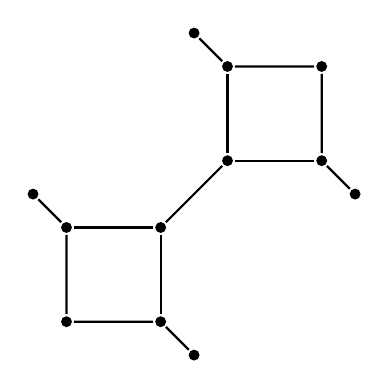
\begin{tikzpicture}[rotate=45,scale=\gscale]
	
	\GraphInit[unit=3,vstyle=Normal]
	%\draw[help lines] (-5,-5) grid (5,5);
	\SetVertexNormal[Shape=circle, FillColor=black, MinSize=2pt]
	\tikzset{VertexStyle/.append style = {inner sep = \inners, outer sep = \outers}}
	\begin{scope}[shift={(-2.41cm, 0cm)}]
	\SetVertexNoLabel
	\grEmptyCycle[RA=1.41,prefix=a]{4}
	\Edges(a0,a1,a2,a3,a0)
	\Vertex[x=0,y=2.41]{1a}
	%\Vertex[y=0,x=-2.41]{2a}
	\Vertex[x=0,y=-2.41]{3a}
	\Edge(1a)(a1)
	%\Edge(2a)(a2)
	\Edge(3a)(a3)
	\end{scope}
	\begin{scope}[shift={(2.41cm, 0cm)}]
	\SetVertexNoLabel
	\grEmptyCycle[RA=1.41,prefix=b]{4}
	\Edges(b0,b1,b2,b3,b0)
	\Vertex[x=0,y=2.41]{1b}
	%\Vertex[y=0,x=2.41]{0b}
	\Vertex[x=0,y=-2.41]{3b}
	\Edge(1b)(b1)
	%\Edge(0b)(b0)
	\Edge(3b)(b3)
	\end{scope}
	\Edge(a0)(b2)
	\end{tikzpicture}
	\hfill
	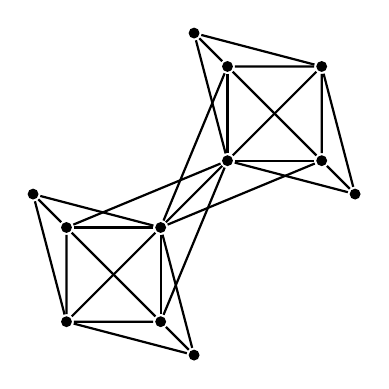
\begin{tikzpicture}[rotate=45,scale=\gscale]
	
	\GraphInit[unit=3,vstyle=Normal]
	%\draw[help lines] (-5,-5) grid (5,5);
	\SetVertexNormal[Shape=circle, FillColor=black, MinSize=2pt]
	\tikzset{VertexStyle/.append style = {inner sep = \inners, outer sep = \outers}}
	\begin{scope}[shift={(-2.41cm, 0cm)}]
	\SetVertexNoLabel
	\grEmptyCycle[RA=1.41,prefix=a]{4}
	\Edges(a0,a1,a2,a3,a0)
	\Vertex[x=0,y=2.41]{1a}
	%\Vertex[y=0,x=-2.41]{2a}
	\Vertex[x=0,y=-2.41]{3a}
	\Edge(1a)(a1)
	%\Edge(2a)(a2)
	\Edge(3a)(a3)
	
	\Edge(a0)(a2)
	\Edge(a1)(a3)
	
	\Edge(1a)(a2)
	\Edge(3a)(a2)
	\Edge(1a)(a0)
	\Edge(3a)(a0)
	%\Edge(2a)(a1)
	%\Edge(2a)(a3)
	\end{scope}
	\begin{scope}[shift={(2.41cm, 0cm)}]
	\SetVertexNoLabel
	\grEmptyCycle[RA=1.41,prefix=b]{4}
	\Edges(b0,b1,b2,b3,b0)
	\Vertex[x=0,y=2.41]{1b}
	%\Vertex[y=0,x=2.41]{0b}
	\Vertex[x=0,y=-2.41]{3b}
	\Edge(1b)(b1)
	%\Edge(0b)(b0)
	\Edge(3b)(b3)
	
	\Edge(b0)(b2)
	\Edge(b1)(b3)
	
	\Edge(1b)(b2)
	\Edge(3b)(b2)
	\Edge(1b)(b0)
	\Edge(3b)(b0)
	%\Edge(0b)(b1)
	%\Edge(0b)(b3)
	\end{scope}
	\Edge(a0)(b2)
	\Edge(a0)(b1)
	\Edge(a0)(b3)
	\Edge(b2)(a1)
	\Edge(b2)(a3)
	\end{tikzpicture}
	\hfill
	\begin{tikzpicture}[shift={(1.41cm,0cm)},rotate=45,scale=\gscale]
	
	\GraphInit[unit=3,vstyle=Normal]
	%\draw[help lines] (-5,-5) grid (5,5);
	\SetVertexNormal[Shape=circle, FillColor=black, MinSize=2pt]
	\tikzset{VertexStyle/.append style = {inner sep = \inners, outer sep = \outers}}
	\begin{scope}[shift={(-2.41cm, 0cm)}]
	\SetVertexNoLabel
	\grEmptyCycle[RA=1.41,prefix=a]{4}
	\Edges(a0,a1,a2,a3,a0)
	\Edge(a0)(a2)
	\Edge(a1)(a3)
	\end{scope}
	\begin{scope}[shift={(2.41cm, 0cm)}]
	\SetVertexNoLabel
	\grEmptyCycle[RA=1.41,prefix=b]{4}
	\Edges(b0,b1,b2,b3,b0)
	\Edge(b0)(b2)
	\Edge(b1)(b3)
	\end{scope}
	\Edge(a0)(b2)
	\Edge(a0)(b1)
	\Edge(a0)(b3)
	\Edge(b2)(a1)
	\Edge(b2)(a3)
	\end{tikzpicture}
	\hfill
	
	
	
	\caption{A triangle-free graph (left), its square (center) and its star graph (right).}
	\label{fig:tri_star}
\end{figure}

Before proceeding to the main results of this chapter, we make the following remark.

\begin{observation}
	Every vertex of degree at least two in a $K_3$-free graph is the center of exactly one maximal star.
\end{observation}

The above observation immediately leads us to the property that every star graph of a triangle-free graph is closely related to the square of one of its induced subgraphs.

\begin{observation}
	If $H$ is a $K_3$-free graph with at least 3 vertices, $D$ are its vertices of degree at least 2 and $G = \K{S}(H)$, it holds that $G \simeq H[D]^2$.
\end{observation}

As such, every hardness result or polynomial time algorithm for the recognition of squares of triangle-free graphs immediately applies to the class of star graphs of triangle-free graphs.
For an illustration of the previous observation, we refer to Figure~\ref{fig:tri_star}.
For a far more complicated star graph, we refer to Figure~\ref{fig:star_example}.



\begin{figure}[!tb]
	\centering
	\begin{tikzpicture}
	\GraphInit[unit=3,vstyle=Normal]
	\SetVertexNormal[Shape=circle, FillColor = black, MinSize=3pt]
	\tikzset{VertexStyle/.append style = {inner sep = \inners,outer sep = \outers}}
	\SetVertexNoLabel
	\begin{scope}[rotate=45]
	\grComplete[RA=1]{4}
	\end{scope}
	\Vertex[x=0, y=-2]{x4}
	\Vertex[x=0, y=-4]{x3}
	\Vertex[x=0, y=-6]{x2}
	\Vertex[x=-1, y=-6]{x1}
	\Edges(a3,x4,a2)
	\Edges(x4,x3,x2,x1)
	\end{tikzpicture}
	\hfill
	\begin{tikzpicture}
	\GraphInit[unit=3,vstyle=Normal]
	\SetVertexNormal[Shape=circle, FillColor = black, MinSize=3pt]
	\tikzset{VertexStyle/.append style = {inner sep = \inners,outer sep = \outers}}
	\SetVertexNoLabel
	\Vertex[x = 0, y = 0.707]{v78}
	\Vertex[x = 2, y = -0.707]{v854}
	\Vertex[x = 1, y = -0.707]{v754}
	
	\Vertex[x = -1, y = -0.707]{v764}
	\Vertex[x = -2, y = -0.707]{v864}
	\Vertex[x = 0, y = 0]{v65}
	
	\Vertex[x = 1, y = -2]{v543}
	
	\Vertex[x = -1, y = -2]{v643}
	
	\Vertex[x = 0, y = -4]{v432}
	
	\Vertex[x = 0, y = -6]{v321}
	
	
	
	\Edge(v65)(v764)
	\Edge(v643)(v854)
	\Edge(v643)(v864)
	\Edge(v321)(v432)
	\Edge(v754)(v854)
	\Edge(v643)(v754)
	\Edge(v543)(v65)
	\Edge(v764)(v78)
	\Edge(v864)(v78)
	\Edge(v543)(v854)
	\Edge(v764)(v754)
	\Edge(v764)(v864)
	\Edge(v432)(v764)
	\Edge(v643)(v65)
	\Edge(v65)(v754)
	\Edge[style = bend right](v864)(v854)
	\Edge(v432)(v643)
	\Edge(v321)(v543)
	\Edge(v643)(v764)
	\Edge(v643)(v543)
	\Edge(v864)(v754)
	\Edge(v754)(v78)
	\Edge(v854)(v78)
	\Edge(v543)(v864)
	\Edge(v543)(v764)
	\Edge(v321)(v643)
	\Edge(v432)(v543)
	\Edge(v65)(v854)
	\Edge(v543)(v754)
	\Edge(v764)(v854)
	\Edge[style=bend right](v432)(v854)
	\Edge[style=bend left](v432)(v864)
	\Edge(v432)(v754)
	\Edge(v65)(v864)
	\end{tikzpicture}
	\hfill
	
	
	
	\caption{A graph (left) and its star graph (right).}
	\label{fig:star_example}
\end{figure}

However, star graphs appear to be natural generalizations of square graphs~\citep{murty} in the sense that, when applying the squaring operation, for each vertex $v$ only the largest, non-induced star centered at $v$ is selected, and the intersection graph of these stars is generated.
On the other hand, for star graphs, every maximal \textit{induced} star is used in the construction of the intersection graph.
Despite the classes of star graphs and biclique graphs being equivalent when restricting the  pre-image domain to $C_4$-free graphs, we were unable to deepen the study of biclique graphs; our efforts were hindered by some of the questions posed and developed upon in this work.



\section{A bound for star-critical pre-images}

Our first results shows an upper bound on the number of vertices of a star-critical graph in terms of its number of maximal stars.
For an arbitrary graph $H$ the difference $|V(H)| - |\str(H)|$ could be arbitrarily big, but some vertices of $H$ would have to be non-star-critical for such a property to occur (e.g. if $H \simeq K_{1,r}$ there are $r-1$ non-star-critical vertices).
In a sense, star-critical graphs are minimal with respect to the star graph obtained with the application of the star operator $\K{S}$.
Recall that maximal star $s_a$ absorbs maximal star $s_b$ if, by removing one leaf of $s_b$, it becomes a substar of $s_a$.

\begin{theorem}
    \label{thm:bound}
    If $H$ is a $n$-vertex star-critical graph, $n \leq \frac{1}{2}\left(3|\str(H)|^2 - |\str(H)|\right)$.
\end{theorem}

\begin{proof}
    We begin by partitioning $V(H)$ in $K = \{v \in V(H) \mid \exists s_a \in \str(H), v = c(s_a)\}$, which contains the center of every maximal star of $H$; and $I = V(H) \setminus K$, which is a subset of its simplicial vertices.
    Note that $I$ is an independent set of $H$, otherwise there would be an edge with endpoints $\{u,v\} \subseteq I$ and either $u$ or $v$ would be in $K$.
    $I$ is partitioned in $I_A, I_E$: the removal of a vertex in $I_A$ cause the absorption of at least one star, the removal of a vertex in $I_E$ causes the disappearance of some edge of the star graph.
    
    $|K| \leq |\str(H)|$ since each maximal star has a center.
    To bound $|I|$, we divide the analysis in the two possible cases for a vertex to be star-critical.
    \begin{itemize}
        \item Suppose that the removal of some $z \in I_A$ causes $s_a$, with $u = c(s_a)$, to be absorbed by $s_b$.
        One of two possibilities arise: if $z$ has only one neighbor then $z$ is the only neighbour of $u$ with this property; therefore there are at most $|K|$ such vertices.
        Otherwise, if $z$ has at least two neighbors, there must be some $v \in N(z) \cap N(u)$ with $v \in s_b \setminus s_a$. However, since $I$ is an independent set, $v \in K$. Therefore, for each maximal star $s_a$, since $H$ is star-critical, there is at most one different $z \in I_A$ for each $v \in (N(u) \cap N(z) \cap K) \setminus s_a$ preventing $v$ from being added to $s_a$.
        This implies that the number of vertices required to avoid absorption is at most $|\str(H)|(|K \setminus \{u\}|) \leq 2\binom{|\str(H)|}{2}$.
        \item For the other condition, each $z \in I_E$ could be responsible for the intersection of a different pair of stars of $H$; i.e., $\exists s_a,s_b \in \str(H)$ such that $s_a \cap s_b = \{z\}$. Since we have $\binom{|\str(H)|}{2}$ pairs, we may have as many vertices in $I$.
    \end{itemize}
    Summing both cases, we have $|I| \leq \frac{3}{2}\binom{|\str(H)|}{2}$ and since $n = |K| + |I|$, it holds that $n \leq \frac{3|\str(H)|^2 - |\str(H)|}{2}$.
\end{proof}

\begin{corollary}
    If $H$ is star-critical and has no simplicial vertex, $|V(H)| \leq |\str(H)|$.
    If the only simplicial vertices of $H$ are leaves, $|V(H)| \leq 2|\str(H)|$.
\end{corollary}

Improvements to the bound given by Theorem~\ref{thm:bound} appear to require a complete characterization of non-star-critical vertices.
Also, a better understanding of vertices that are required only for the intersection of some stars to be non-empty seems necessary in order to approach the problem through induction.
We believe that a reasonable bound would be of the form $|V(H)| \leq 2|V(G)| + \sqrt{|E(G)|}$, where $G \simeq \K{S}(H)$.

\begin{conjecture}
    For every star-critical graph $H$ and its star graph $G$, it holds that $|V(H)| \leq 2|V(G)| + \sqrt{|E(G)|}$.
\end{conjecture}

If this result indeed holds, it would configure an important difference from other intersection graphs.
For instance, there are clique-critical graphs which require a quadratic number of vertices on the pre-image~\cite{clique_critical_alcon}.
However, we conjecture an even stronger result, which we back with the experiments we describe later in this chapter.

\begin{conjecture}
	For every star-critical graph $H$ and its star graph $G$, it holds that $|V(H)| \leq 2|V(G)|$.
\end{conjecture}
\section{Characterization}


Much of the following discussion will be about edge clique covers, a central piece on the characterization of many intersection graph classes.
We denote this family of subgraphs of $G$ by $\mathcal{Q} = \{Q_1, \dots, Q_n\}$.
The usual strategy in these constructions is to use each clique as a vertex of the pre-image; this is also our approach.
Since each vertex $a \in V(G)$ must be a star in $H$, it is reasonable to partition each clique as $Q_i \sim \{Q_i^c, Q_i^f\}$, that is, the vertices $a \in Q_i^c$ correspond to the stars of $G$ with center in $v_i \in V(H)$, while the vertices $a \in Q_i^f$ correspond to the stars of $G$ where $v_i \in V(H)$ is a leaf.
We call such an edge clique cover a \tdef{star-partitioned edge clique cover} of $\mathcal{Q}$.

To simplify our notation, for each $a \in V(G)$, we denote its \tdef{center} by $c(a)$, i.e. $c(a)$ is the unique $i$ such that $a \in Q_i^c$, its \tdef{leaf set} by $F(a) = \{i \mid a \in Q_i^f\}$ and its \tdef{cover} by $Q(a) = F(a) \cup \{c(a)\}$. For each pair of cliques $Q_i, Q_j \in \mathcal{Q}$, their \tdef{leaf-leaf intersection} is given by $\ff(i,j) = Q_i^f \cap Q_j^f$ and its \tdef{center-leaf intersection} by $\cf(i,j) = \left(Q_i^c \cap Q_j^f\right) \cup \left(Q_i^f \cap Q_j^c\right)$.

\begin{definition}[Star-compatibility]
    Given a graph $G$ and a star-partitioned edge clique cover $\mathcal{Q}$ of $G$, we say that $\mathcal{Q}$ is \tdef{star-compatible} if, for every $a \in V(G)$, $|Q(a)| \geq 2$, $\exists!\ i$ such that $a \in Q_i^c$ and if, for every $Q_i, Q_j \in \mathcal{Q}$, if $Q_i \cap Q_j \neq \emptyset$, either $\cf(i,j) = \emptyset$ or $\ff(i,j) = \emptyset$.
\end{definition}

\begin{definition}[Star-differentiability]
    \label{def:differentiability}
    Given a graph $G$ and a star-partitioned edge clique cover $\mathcal{Q}$ of $G$, we say that $\mathcal{Q}$ is \tdef{star-differentiable} if for every $Q_i \in \mathcal{Q}$ and for every pair $\{a, a'\} \subseteq Q_i$ the following conditions hold:
    \begin{enumerate}
        \item If $\{a, a'\} \subseteq Q_i^c$, there exists $Q_j, Q_k \in \mathcal{Q}$ such that $a \in Q_j^f$, $a' \in Q_k^f$, $a \notin Q_k^f$, $a' \notin Q_j^f$ and $\cf(j,k) \neq \emptyset$. Moreover, if $Q_i^c \cap Q_j^f \cap Q_k^f = \emptyset$, $\cf(j,k) \neq \emptyset$.
        \item If $a \in Q_i^c$, $a' \in Q_k^c$ and $a \notin Q_k^f$, then there is some $j \in F(a)$ with $\cf(j,k) \neq \emptyset$, $j \notin Q(a')$ and, for every $j' \in F(a)$ with $\cf(j',k) = \emptyset$, $Q_i^c \cap \bigcap_{j'} \ff(j',k) \neq \emptyset$.
        \item If $a \in Q_i^c$, $a' \in Q_k^c$ and $a \in Q_k^f$, for every $j \in F(a) \setminus \{k\}$, $\cf(j,k) = \emptyset$.
        \item If $\{a, a'\} \subseteq Q_i^f$ and $j = c(a) \neq c(a') = k$, then either $Q_i^c \cap \ff\left(j,k\right) \neq \emptyset$ or $\cf\left(j,k\right) \neq \emptyset$.
    \end{enumerate}
\end{definition}

Figures~\ref{fig:diff_cases} and~\ref{fig:diff_cases2} show the four cases of Definition~\ref{def:differentiability} as seen on the pre-image of the star graph we shall build from $\mathcal{Q}$.

\begin{figure}[!htb]
    \centering
            \begin{tikzpicture}[scale=\gscale]
                %\draw[help lines] (-5,-5) grid (5,5);
                \begin{scope}[shift={(0cm,1cm)}]
                    \GraphInit[unit=3,vstyle=Normal]
                    \SetVertexNormal[Shape=circle, FillColor=black, MinSize=2pt]
                    \tikzset{VertexStyle/.append style = {inner sep = \inners, outer sep = \outers}}
                    \Vertex[Math,Ldist=3pt,Lpos=90,LabelOut,L={i},x=0,y=0]{i1}
                    \Vertex[Math,Ldist=3pt,Lpos=180,LabelOut,L={j},a=150, d=2]{j1}
                    \Vertex[Math,Ldist=3pt,Lpos=0,LabelOut,L={k},a=30, d=2]{k1}
                    \node[] at (-0.6,-0.35) {$a$};
                    \node[] at (0.6,-0.31) {$a'$};
                    \Vertex[Math,x=0,y=-2,Ldist=3pt,Lpos=270,LabelOut,L={j'}]{r1};
                    
                    \Edge(i1)(j1)
                    \Edge(i1)(r1)
                    \Edge(i1)(k1)
                    \Edge(j1)(k1)
                    \Edge[style=dotted](j1)(r1)
                    \Edge[style=dotted](k1)(r1)
                \end{scope}
            \end{tikzpicture}
    \hfill
            \begin{tikzpicture}[scale=\gscale]
                %\draw[help lines] (-5,-5) grid (5,5);
                \begin{scope}[shift={(0cm,0cm)}]
                    
                    \GraphInit[unit=3,vstyle=Normal]
                    \SetVertexNormal[Shape=circle, FillColor=black, MinSize=2pt]
                    \tikzset{VertexStyle/.append style = {inner sep = \inners, outer sep = \outers}}
                    \Vertex[Math,Ldist=3pt,Lpos=110,LabelOut,L={i},x=0,y=0]{i2}
                    \Vertex[Math,Ldist=3pt,Lpos=180,LabelOut,L={j},a=150, d=2]{j2}
                    \Vertex[Math,Ldist=3pt,Lpos=0,LabelOut,L={k},a=30, d=2]{k2}
                    \node[] at (-0.6,-0.35) {$a$};
                    \node[] at (1.23,1.50) {$a'$};
                    \Vertex[Math,Ldist=3pt,Lpos=270,LabelOut,L={j'},x=0,y=-2]{j'2};
                    \SetVertexNoLabel
                    \Vertex[x=1.73,y=3]{r2}
                    
                    \Edge(i2)(j2)
                    \Edge(i2)(j'2)
                    \Edge(i2)(k2)
                    \Edge(j2)(k2)
                    \Edge(r2)(k2)
                    \Edge[style=dotted](j2)(j'2)
                    \Edge[style=dotted](k2)(j'2)
                    \Edge[style=dotted](i2)(r2)
                \end{scope}
            \end{tikzpicture}
    \hfill
            \begin{tikzpicture}[rotate=180,scale=\gscale]
                %\draw[help lines] (-5,-5) grid (5,5);
                \begin{scope}[shift={(0cm,0cm)}]
                    \GraphInit[unit=3,vstyle=Normal]
                    \SetVertexNormal[Shape=circle, FillColor=black, MinSize=2pt]
                    \tikzset{VertexStyle/.append style = {inner sep = \inners, outer sep = \outers}}
                    \Vertex[Math,Ldist=3pt,Lpos=90,LabelOut,L={i},x=0,y=0]{i3}
                    \Vertex[Math,Ldist=3pt,Lpos=90,LabelOut,L={j},a=150, d=2]{j3}
                    \Vertex[Math,Ldist=3pt,Lpos=90,LabelOut,L={k},a=30, d=2]{k3}
                    \SetVertexNoLabel
                    \Vertex[Math,Ldist=3pt,Lpos=0,LabelOut,L={k},a=30, d=4]{r3}
                    \Vertex[Math,Ldist=3pt,Lpos=0,LabelOut,L={k},x=0, y=2]{l3}
                    \node[] at (0,0.6) {$a$};
                    \node[] at (1.73,1.6) {$a'$};
                    
                    \Edge(i3)(j3)
                    \Edge(i3)(k3)
                    \Edge[style=dotted](j3)(k3)
                    \Edge(k3)(r3)
                    \Edge(k3)(l3)
                    \Edge[style=dotted](r3)(l3)
                \end{scope}
            \end{tikzpicture}
    \hfill
    
    
    
    \caption{The first three cases of Definition~\ref{def:differentiability}. The first (left), second (center) and third (right).}
    \label{fig:diff_cases}
\end{figure}


\begin{figure}[!htb]
    \centering
    
        \begin{tikzpicture}[scale=\gscale]
            
            \begin{scope}[shift={(-4cm,-1cm)}, rotate=180]
                \GraphInit[unit=3,vstyle=Normal]
                \SetVertexNormal[Shape=circle, FillColor=black, MinSize=2pt]
                \tikzset{VertexStyle/.append style = {inner sep = \inners, outer sep = \outers}}
                \Vertex[Math,Ldist=3pt,Lpos=90,LabelOut,L={i},x=0,y=0]{i4}
                \Vertex[Math,Ldist=3pt,Lpos=90,LabelOut,L={k_1},a=150, d=2]{j4}
                \Vertex[Math,Ldist=3pt,Lpos=90,LabelOut,L={j_1},a=30, d=2]{k4}
                
                
                \SetVertexNoLabel
                \Vertex[Math,Ldist=3pt,Lpos=0,LabelOut,L={k},a=30, d=4]{r4}
                \Vertex[Math,Ldist=3pt,Lpos=0,LabelOut,L={k},x=0.4, y=2]{l4}
                \Vertex[Math,Ldist=3pt,Lpos=0,LabelOut,L={k},a=150, d=4]{m4}
                \Vertex[Math,Ldist=3pt,Lpos=0,LabelOut,L={k},x=-0.4, y=2]{n4}
                
                
                \node[] at (-1.77,1.5) {$a_1'$};
                \node[] at (1.77,1.5) {$a_1$};
                
                \Edge(i4)(j4)
                \Edge(i4)(k4)
                \Edge[style=dotted](j4)(k4)
                \Edge(k4)(r4)
                \Edge(k4)(l4)
                \Edge[style=dotted](r4)(l4)
                \Edge(j4)(n4)
                \Edge(j4)(m4)
                \Edge[style=dotted](m4)(n4)
                
                
            \end{scope}
        \end{tikzpicture}
        \hfill
        \begin{tikzpicture}[scale=\gscale]
            \begin{scope}[shift={(4cm,1cm)}]
                \GraphInit[unit=3,vstyle=Normal]
                \SetVertexNormal[Shape=circle, FillColor=black, MinSize=2pt]
                \tikzset{VertexStyle/.append style = {inner sep = \inners, outer sep = \outers}}
                \Vertex[Math,Ldist=3pt,Lpos=90,LabelOut,L={i},x=0,y=0]{i5}
                \Vertex[Math,Ldist=3pt,Lpos=90,LabelOut,L={j_2},a=210, d=2]{j5}
                \Vertex[Math,Ldist=3pt,Lpos=90,LabelOut,L={k_2},a=-30, d=2]{k5}
                
                
                
                \SetVertexNoLabel
                
                
                \Vertex[Math,Ldist=3pt,Lpos=0,LabelOut,L={k},a=-30, d=4]{r5}
                \Vertex[Math,Ldist=3pt,Lpos=0,LabelOut,L={k},x=0.4, y=-2]{l5}
                \Vertex[Math,Ldist=3pt,Lpos=0,LabelOut,L={k},a=210, d=4]{m5}
                \Vertex[Math,Ldist=3pt,Lpos=0,LabelOut,L={k},x=-0.4, y=-2]{n5}
                
                \node[] at (-1.77,-1.5) {$a_2$};
                \node[] at (1.77,-1.5) {$a'_2$};
                
                
                \Edge(i5)(j5)
                \Edge(i5)(k5)
                \Edge(j5)(k5)
                \Edge(k5)(r5)
                \Edge(k5)(l5)
                \Edge[style=dotted](r5)(l5)
                \Edge(j5)(n5)
                \Edge(j5)(m5)
                \Edge[style=dotted](m5)(n5)
                
            \end{scope}
        \end{tikzpicture}
    
    
    
    \caption{The fourth case of Definition~\ref{def:differentiability}.}
    \label{fig:diff_cases2}
\end{figure}


We emphasize that: (i) star-compatibility translates the structural properties of stars; and (ii) star-differentiability enumerates the possible ways that two stars that share at least one vertex are different.
Note that, the \say{missing case}, where $\{a,a'\} \in Q_i^f$ and $c(a) = c(a') = k$ is exactly the same case as 1, but with $\{a,a'\} \in Q_k^c$ instead of $Q_i^c$.

\begin{lemma}
    \label{lem:star_maximality}
    Let $G$ be a graph and $\mathcal{Q}$ a star-partitioned edge clique cover of $G$. If $\mathcal{Q}$ is star-compatible and star-differentiable then, for every pair $\{a, a'\} \subseteq V(G)$, $Q(a) \nsubseteq Q(a')$ and $Q(a') \nsubseteq Q(a)$.
\end{lemma}

\begin{tproof}
    If $a$ and $a'$ do not share any clique, the result is trivial.
    
    Otherwise they do share some clique, say $Q_i$.
    For properties 1, 2 and 4 of Definition~\ref{def:differentiability}, we conclude that $i \in Q(a) \cap Q(a')$ and that $j \in Q(a)$, $k \in Q(a')$ but $j \notin Q(a')$ and $k \notin Q(a)$, which implies $Q(a) \nsubseteq Q(a')$ and $Q(a') \nsubseteq Q(a)$.
    
    For property 3, however, we first conclude that there is some $j \in Q(a)$ but $j \notin Q(a')$, otherwise we would have $\cf(j,k) \neq \emptyset$ and $\ff(j,k) \neq \emptyset$.
    Consequently, $Q(a) \nsubseteq Q(a')$.
    For the converse, we note that $\{a, a'\} \subseteq Q_k$ and, following the same argument, we conclude that there is $j' \in Q(a')$ but $j' \notin Q(a)$ and, finally, that $Q(a') \nsubseteq Q(a)$.
\end{tproof}

We now present a Krausz-type characterization for the class of star graphs.

\begin{theorem}
    \label{thm:star_characterization}
    An $n$-vertex graph $G$ is the star graph of some graph $H$ if and only if there is a star-compatible and star-differentiable star-partitioned edge clique cover $\mathcal{Q}$ of $G$ with at most $\frac{1}{2}(3n^2 - n)$ cliques.
\end{theorem}

\begin{tproof}
    In this proof, we assume that $H$ has $m$ vertices ($v_i$). For simplicity, a star $s_a \in \str(H)$ corresponds to the vertex $a \in V(G)$.
    
    For the first direction of the statement, assume $H$ is a star-critical pre-image of $G$.
    For each $v_i \in V(H)$, let $S(v_i) = \{s_a \in \str(H) \mid v_i \in s_a\}$, that is, the maximal stars of $H$ that contain $v_i$.
    Clearly, we can partition these sets as $S(v_i) \sim \{S^c(v_i), S^f(v_i)\}$, that is, the stars where $v_i$ is the center and where it is a leaf, respectively.
    Our goal is to show that $\mathcal{Q} = \{Q_1, \dots, Q_m\}$, with $Q_i^c = S^c(v_i)$ and $Q_i^f = S^f(v_i)$ is a star-partitioned edge clique cover of $G$ satisfying star-compatibility and star-differentiability which, by Theorem~\ref{thm:bound}, is all that remains is to be proven, since $|\mathcal{Q}| = |V(H)| \leq \frac{1}{2}(3n^2 - n)$.
    
    To verify that $\mathcal{Q}$ is a star-partitioned edge clique cover of $G$, first note that every $Q_i$ is a clique of $G$, since the corresponding stars share at least $v_i \in V(H)$.
    For the coverage part, every $aa' \in E(G)$ has two corresponding stars $s_a, s_{a'} \in \str(H)$, which share at least one vertex, say $v_i \in V(H)$, since $G \simeq \K{S}(H)$.
    By the construction of $\mathcal{Q}$, there is some $Q_i \in \mathcal{Q}$ which corresponds to every maximal star that contains $v_i$; this guarantees that $aa'$ is covered by at least one clique of $\mathcal{Q}$.
    
    For the other properties, first take two vertices $v_i,v_j \in V(H)$ with $v_iv_j \notin E(H)$ but $S(v_i) \cap S(v_j) \neq \emptyset$.
    Clearly, no star in $S(v_i) \cap S(v_j)$ may have $v_i$ and $v_j$ in different sides of its bipartition, thus $S(v_i) \cap S(v_j) = S^f(v_i) \cap S^f(v_j)$.
    Now, suppose that $v_iv_j \in E(H)$; since they are adjacent, any star in $S(v_i) \cap S(v_j)$ must have $v_i$ and $v_j$ in opposite sides of the bipartition and, thus, we have that $S(v_i) \cap S(v_j) = \left(S^c(v_i) \cap S^f(v_j)\right) \cup \left(S^f(v_i) \cap S^c(v_j)\right)$.
    Since each star has a single center, the above analysis shows that $\mathcal{Q}$ satisfies star-compatibility.
    
    For star-differentiability, let $\{s_a, s_{a'}\} \subseteq S(v_i)$. We break our analysis in the same order as the one given in Definition~\ref{def:differentiability}.
    \begin{enumerate}
        \item If $\{s_a, s_{a'}\} \subseteq S^c(v_i)$ there must be at least one leaf in each star, say $v_j$ and $v_k$, respectively, not in the other and these leaves must be adjacent to each other, otherwise at least one of the stars would not be maximal.
        That is, $\{a, a'\} \in Q_i^c$ imply that there is $Q_j,Q_k \in \mathcal{Q}$ with $a \in Q_j^f$, $a' \in Q_k^f$, $a \notin Q_k^f$, $a \notin Q_j^f$ and $\cf(j,k) \neq \emptyset$.
        \item If $s_a \in S(v_i)^c$, $s_{a'} \in S(v_k)^c$ and $s_a \notin S(v_k)^f$, $v_iv_k \in E(H)$ and to keep $v_k$ from being a leaf of $s_a$, one leaf of $s_a$, say $v_j$, must also be adjacent to $v_k$ and not a leaf of $s_{a'}$, since $v_i$ is.
        Now, for every $v_{j'} \in s_a$ and not adjacent to $v_k$, there is a clear $P_3 = v_kv_iv_{j'}$, which must be part of some maximal star.
        Moreover, the set of all $v_{j'}$ non-adjacent to $v_k$ will form a maximal star centered around $v_i$ along with $v_k$.
        Thus, $a \in Q_i^c$, $a' \in Q_k^c$ and $a \notin Q_k^f$, imply that there is some $j \in F(a)$ with $\cf(j,k) \neq \emptyset$, $j \notin Q(a')$ and, for $j' \in F(a)$ with $\cf(j', k) = \emptyset$, $Q_i^c \cap \bigcap_{j'} \ff(j',k) \neq \emptyset$.
        \item If $s_a \in S(v_i)^c$, $s_{a'} \in S(v_k)^c$ and $s_a \in S(v_k)^f$, we know that $s_a = \{v_i\}\{v_k, \dots\}$ and, since $v_k$ is not adjacent to any other leaf $v_j$ of $s_a$, we know that $S(v_j) \cap S(v_k) = S^f(v_j) \cap S^f(v_k)$ and, since $v_k$ is the center of $s_{a'}$, $v_j$ is not one of its leaves.
        Therefore, $a \in Q_i^c$, $a' \in Q_k^c$ and $a \in Q_k^f$, implies that for every $j \in F(a) \setminus \{k\}$, $\cf(j,k) = \emptyset$.
        \item If $\{s_a, s_{a'}\} \subseteq Q_i^f$ and $s_a \in S^c(v_j)$, $s_{a'} \in S^c(v_k)$, either $v_jv_k \notin E(H)$, which induces the existence a star $\{v_i\}\{v_j, v_k, \dots\}$, or $v_jv_k \in E(H)$, which must be part of a star with either $v_j$ or $v_k$ as center and the other as a leaf.
        Hence, $\{a, a'\} \subseteq Q_i^f$ and $j = c(a) \neq c(a') = k$, implies that either $Q_i^c \cap \ff\left(j,k\right) \neq \emptyset$ or $\cf\left(j,k\right) \neq \emptyset$.
    \end{enumerate}
    The above shows that $\mathcal{Q}$ is also star-differentiable, which completes this part of the proof.
    
    For the converse, take $\mathcal{Q}$ a star-partitioned edge clique cover of $G$ satisfying star-compatibility and star-differentiability  of size at most $\frac{1}{2}(3n^2 - n)$ and let $H$ be a graph with $V(H) = \{v_i \mid Q_i \in \mathcal{Q}\}$ and $E(H) = \{v_iv_j \mid \cf(i,j) \neq \emptyset\}$ and let us prove that $G \simeq \K{S}(H)$.
    
    Take $a \in V(G)$ with $c(a) = i$.
    Due to star-compatibility and the construction of $H$, we know that $H[\{v_j \mid j \in F(a)\}]$ is an independent set of $H$ and that $s_a = \{v_i\}\{v_j \mid j \in F(a)\}$ is a star of $H$.
    Suppose, however, that $s_a$ is not maximal, that is, there is some $v_k \in V(H)$ such that $v_iv_k \in E(H)$ and $s_b = s_a \cup \{v_k\}$ is a star of $H$.
    By the construction of $H$, either there is some $a' \in V(G)$ such that $Q(a) \subseteq Q(a')$, which is impossible due to Lemma~\ref{lem:star_maximality}, or some $a' \in \cf(i,k)$, which we analyze below.
    The following is based on the first two cases of Definition~\ref{def:differentiability}; the other two are impossible, since $k \notin Q(a)$ and $a \in Q_i^c$.
    
    \begin{enumerate}
        \item If $a' \in Q_i^c$, there is some $Q_j \in \mathcal{Q}$ such that $a \in Q_j^f$ and $\cf(j,k) \neq \emptyset$, which implies that $v_jv_k \in E(H)$ and $s_b$ is not a star of $H$. 
        \item If $a' \in Q_k^c$ and $a \notin Q_k^f$, at least one $j \in F(a)$ satisfies $\cf(j,k) \neq \emptyset$ and $j \notin Q(a')$.
        This gives us that $v_jv_k \in E(H)$ and $s_b$ is not a star of $H$.
    \end{enumerate}
    
    Therefore, we conclude that $a'$ cannot exist, that $s_a$ is maximal and, consequently that $V(G) \subseteq V(\K{S}(H))$.
    
    To show that $V(\K{S}(H)) \subseteq V(G)$, take $s = \{v_i\}L$, with $s \in \str(H)$, and suppose that there is some $j,k \in L$ and that for every pair $a \in \cf(i,j)$ and $a' \in \cf(i,k)$, $a \notin Q_k$ and $a' \notin Q_j$.
    That is, $Q_i \cap Q_j \cap Q_k = \emptyset$, due to star-compatibility and the hypothesis that $jk \notin E(H)$.
    Once again, we analyze the possibilities in terms of Definition~\ref{def:differentiability}.
    
    \begin{enumerate}
        \item If $c(a) = c(a') = i$, we have that $\cf(j,k)  \neq \emptyset$, implying that $v_jv_k \in E(H)$, contradicting the hypothesis that $s$ exists.
        \item If $c(a) = i$ and $c(a') = k$, there is some $j' \in Q(a)$ with $\cf(j,k) \neq \emptyset$. To conclude that $j = j'$, we note that, if $j \neq j'$, it would be required that $Q_i^c \cap \ff(j,k) \neq \emptyset$, which is impossible since $Q_i \cap Q_j \cap Q_k = \emptyset$.
        Once again, contradicting the hypothesis that such an $s$ exists.
        \item Trivially impossible since $Q_i \cap Q_j \cap Q_k = \emptyset$.
        \item If $j = c(a) \neq c(a') = k$, either $Q_i^c \cap \ff(j,k) \neq \emptyset$, which is impossible since $Q_i \cap Q_j \cap Q_k = \emptyset$, or $\cf(j,k) \neq \emptyset$, implies that $v_jv_k \in E(H)$ and that $s$ is not a star.
    \end{enumerate}
    
    The above allows us to conclude that there is no $s \in \str(H)$ generated by cliques not pairwise intersecting.
    Such intersection has a unique vertex of $G$ in it due to Lemma~\ref{lem:star_maximality}, which allows us to conclude $V(\K{S}(H)) \subseteq V(G)$ and, consequently, that $V(\K{S}(H)) = V(G)$.
    
    To show that $E(G) \subseteq E(\K{S}(H))$, we first take an edge $ab \in E(G)$.
    Since $\mathcal{Q}$ is a star-partitioned edge clique cover of $G$, there is some $i$ such that $\{a,b\} \subseteq Q_i$ and, because $V(G) = V(\K{S}(H))$ and the construction of $H$, there are corresponding stars $s_a, s_b \in \str(H)$ with $v_i \in s_a \cap s_b$ which guarantee that $ab \in E(\K{S}(H))$.
    For $E(\K{S}(H)) \subseteq E(G)$, take two intersecting stars $s_a,s_b \in \str(H)$ and note that, since $a,b \in \K{S}(H) = V(G)$ and $\mathcal{Q}$ is a star-partitioned edge clique cover of $G$, $ab \in E(G)$ and we conclude that $E(G) = E(\K{S}(H))$, completing the proof.
\end{tproof}

We now pose a version of the decision problem for star graph recognition, which we call \textsc{star graph}, and will be the subject of further study.
We will further require that the output for any algorithm for \textsc{star graph} is already star-partitioned.

\problem{Star Graph}{A graph $G$.}{Is there a star-partitioned edge clique cover $\mathcal{Q}$ of $G$ satisfying star-compatibility and star-differentiability?}

Theorem~\ref{thm:star_characterization} provides a straightforward verification algorithm to check if a star-partitioned edge clique cover is star-compatible and star-differentiable.

\begin{theorem}
    \label{thm:verification_alg}
    Given a graph $G$ of order $n$, there is an $\bigO{\max\{n^2m, m^2\}n^2m}$ algorithm to decide if a star-partitioned family $\mathcal{Q} \subseteq 2^{V(G)}$ of size $m$ is an edge clique cover of $G$ satisfying star-compatibility and star-differentiability. 
\end{theorem}

\begin{tproof}
    The first task is to determine whether or not $\mathcal{Q}$ is a star-partitioned edge clique cover of $G$.
    The usual $n^2$ algorithm that tests if each $Q_i$ is a clique suffices.
    To check if $\mathcal{Q}$ is an edge clique cover, for each of the $\bigO{n^2}$ edges, we test if one of the $n$ cliques contains it. 
    This simple test takes $\bigO{n^2m}$ time.
    
    To check for star-compatibility: first, for each vertex $a$ of $G$ and each clique $Q_i$, verify if there is a single $i$ such that $a \in Q_i^c$ and at least one $j$ with $a \in Q_j^f$;
    afterwards, for each pair of intersecting cliques $Q_i, Q_j$, test if $\cf(i,j) = \emptyset$ or $\ff(i,j) = \emptyset$.
    The entire process takes $\bigO{nm^2}$ time.
    
    For star-differentiability, we assume that every pairwise intersection of $\mathcal{Q}$ has already been computed in time $\bigO{nm^2}$, and each query $\cf(j,k)$ and $\ff(j,k)$ takes $\bigO{1}$ time.
    Now, for each clique $Q_i$ and for each pair of vertices $\{a, a'\} \in Q_i$, we must check one of the four conditions as follows.
    \begin{enumerate}
        \item If $c(a) = c(a') = i$, for each pair $j \in Q(a)$, $k \in Q(a')$, check if $a' \notin Q_j^f$, $a \notin Q_k^f$ and $\cf(j,k) \neq \emptyset$; this case takes $\bigO{n^2}$.
        \item If $c(a) = i, c(a') = k$ and $a \notin Q_k^f$, for each $j \in F(a)$, check if either $\cf(j,k) \neq \emptyset$ and $j \notin Q(a')$ or $\cf(j,k) = \emptyset$ and $Q_i^c \cap \ff(j,k) \neq \emptyset$; this case takes $\bigO{n^2m}$ time.
        \item If $c(a) = i, c(a') = k$ and $a \in Q_k^f$, check for each $j \in F(a) \setminus \{k\}$, if $\cf(j,k) = \emptyset$, taking $\bigO{n}$ time.
        \item If $j = c(a) \neq c(a') = k$, we check if $Q_i^c \cap \ff(j,k) \neq \emptyset$ in $\bigO{n}$ time, and if $\cf(j,k)$ in $\bigO{1}$ time.
    \end{enumerate}
    In the worst case scenario, we will spend $\bigO{\max{n^2m, m^2}}$ time for each $Q_i$ and each pair $\{a, a'\} \subseteq Q_i$, of which there are $\bigO{n^2m}$ combinations, and conclude that the whole algorithm takes no more than $\bigO{\max\{n^2m, m^2\}n^2m}$ time.
\end{tproof}

Together with Theorem~\ref{thm:bound}, Theorem~\ref{thm:verification_alg} implies that deciding whether or not a graph is a star graph is in $\mathsf{NP}$, as we summarize in the following statement.

\begin{theorem}
    \textsc{Star Graph} is in $\mathsf{NP}$.
\end{theorem}
\section{Properties}
The next theorem uses the known result, due to~\cite{moon_moser}, that a graph of order $n$ has at most $3^{n/3}$ maximal independent sets.

\begin{theorem}
    If $G$ is the star graph of an $n$ vertex graph $H$, then $|V(G)| \leq n3^{\Delta(H)/3}$.
\end{theorem}

\begin{tproof}
    For every $v \in V(H)$, define $H_v = H[N(v)]$ and note that each maximal independent set of $H_v$ might induce a maximal star of $H$ centered around $v$.
    Since $|V(H_v)| \leq \Delta(H)$, we have that $H_v$ has at most $3^{\Delta(H)/3}$ maximal independent sets and, therefore, $H$ has at most $3^{\Delta(H)/3}$ maximal stars centered around $v$.
    Summing for every $v \in V(H)$ we arrive at the $n3^{\Delta(H)/3}$ bound.
\end{tproof}

The observation made in the proof of the previous theorem is quite useful when one wants to generate $\str(H)$.
In fact, we can do that with \textit{polynomial delay}, i.e., the time between outputting two maximal stars is upper bounded by a polynomial on the size of the graph.
To do so, we employ the polynomial delay algorithm for maximal independent sets of~\cite{independent_poly_delay}.

\begin{theorem}
    There exists an algorithm that, given a graph $H$ on $n$ vertices, generates $\str(H)$ such that the time between the output of two successive members of $\str(H)$ is bounded by a polynomial in $n$.
\end{theorem}

\begin{proof}
    Let $i(n)$ denote the delay between the generation of two maximal independent sets on a graph with $n$ vertices.
    First, we can test for each edge $uv \in E(H)$ if $\{u\}\{v\}$ is a maximal star of $H$: this is the case if and only if $u$ and $v$ are a pair of true twin vertices.
    After this step is done, we have all maximal stars of size two and, since there is a polynomial number of stars of this size, we have polynomial delay.
    Now for each vertex $v \in V(H)$ we use the polynomial delay algorithm of~\cite{independent_poly_delay} to generate all the maximal independent sets of $H_v = H[N(v)]$, discarding all generated independent sets of size one.
    Essentially, this step generates all maximal induced stars of size at least three centered at $v$ and, moreover, the delay between the output of two distinct stars is at most $i(n)n$, since $H_v$ may only have independent sets of size one.
    Finally, this delay of $i(n)n$ may occur for roughly each $H_v$, yielding a total delay of the order $i(n)n^2$.
\end{proof}

\begin{theorem}
    \label{thm:star_cutless}
    If $G$ is a connected star graph, $G$ has no cut-vertex.
\end{theorem}

\begin{tproof}
    If $|V(G)| \leq 4$, we are done as there are only 5 graphs that satisfy these constraints and none of them contain a cut-vertex.
    They are $K_1$, $K_2$, $K_3$, $K_4$ and $K_4$ with one missing edge (the diamond).
    The first three are trivial, while the last two are shown in Figure~\ref{fig:four_star}.
    
    For graphs with 5 or more vertices, suppose that there is some cut-vertex $x \in G$, that $A,B$ are two of the connected components obtained after removing $x$ from $G$ and take a pair of vertices $a \in V(A) \cap N(x)$, $b \in V(B) \cap N(x)$.
    Suppose now that $G = \K{S}(H)$ for some $H$ and take the stars $s_a, s_b, s_x$ corresponding to $a, b, x$, respectively.
    Since $ab \notin E(G)$ and $ax, bx \in E(G)$, it holds that $s_a \cap s_x \neq \emptyset$ and $s_b \cap s_x \neq \emptyset$ but $s_a \cap s_b = \emptyset$.
    
    If $c(a) = c(x) = i$ and $k = c(b) \neq c(x)$, $s_x$ and $s_b$ share at least one leaf, say $v_j$, since they intercept at some vertex, and $v_j \notin s_a$.
    However, there is no leaf $v_{j'} \in s_a$ adjacent to $v_j$, otherwise there would be an edge $v_jv_{j'} \in E(H)$ and, consequently, some star $s_y$, corresponding to vertex $y \in V(G)$, that keeps $A,B$ connected and intercepts $s_a, s_b, s_x$.
    Therefore, we conclude that no leaf of $s_a$ is adjacent to $v_j$ and, since $c(a) = c(x)$ and $v_iv_j \in E(H)$, we conclude that $v_j \in s_a$, otherwise it would not be maximal, and, consequently, $v_j \in s_a \cap s_b$ and $ab \in E(H)$, which contradicts the hypothesis that $A,B$ are disconnected after removing $x$.
    The case where $c(x) = c(b) \neq c(a)$ follows the exact same argument.
    
    Now if $c(a) \neq c(x) = i$ and $c(x) \neq c(b)$, it is easy to see that $v_i$ cannot be a leaf of both $s_a$ and $s_b$ simultaneously, otherwise $v_i \in s_a \cap s_b$ and $ab \in E(H)$.
    So we have two cases to analyze:
    \begin{enumerate}
        \item If $v_i$ is a leaf of $s_a$, $v_j \in s_x \cap s_b$ and $k = c(b)$, clearly $s_y = \{v_j\}\{v_i, v_k, \dots \}$ is a maximal star of $H$ that intercepts $s_a, s_b, s_x$, keeping $A,B$ from being disconnected.
        The case where $v_i$ is a leaf $s_b$ is the same, and we omit it for brevity.
        \item If $v_i$ not a leaf of neither $s_a$ nor $s_b$, $c(a) = j$ and $c(b) = k$, we have leaves $v_{j'} \in s_a \cap s_x$ , $v_{k'} \in s_b \cap s_x$ which form at least two intercepting maximal stars, $s_{a'} = \{v_{j'}\}\{v_i, v_j, \dots\}$ and $s_{b'} = \{v_{k'}\}\{v_i, v_k, \dots\}$, such that $s_{a'} \cap s_a \cap s_x \neq \emptyset$ and $s_{b'} \cap s_b \cap s_x \neq \emptyset$.
    \end{enumerate}
    
    These cases allow us to conclude that $A,B$ remains connected no matter the configuration of the intersection of the corresponding stars in $H$.
    Consequently, $x$ cannot exist and we complete the proof.
\end{tproof}


\begin{theorem}
    Every edge of a star graph $G$ is contained in at least one triangle if $|V(G)| \geq 3$.
\end{theorem}

\begin{tproof}
    The only connected star graph with 3 vertices is $K_3$, so take $G$ with $|V(G)| \geq 4$.
    Take a pre-image $H$ of $G$, $ab \in E(G)$, $s_a, s_b \in \str(H)$ the corresponding stars to $a, b$, and assume that $ab$ is not contained in any triangle of $G$.
    Since $G$ is connected, there is at least one $x \in V(G)$ adjacent to (w.l.o.g) $a$, but not to $b$, and a corresponding maximal star $s_x$ of $H$.
    Below, we analyze the possible intersections between $s_a$ and $s_b$ and conclude that there is always some star $s_y$ that shares one vertex with $s_a$ and $s_b$.
    \begin{enumerate}
        \item If $c(a) = c(b) = i$ and the center of $s_x$ is a leaf of $s_a$, clearly $v_i$ is not a leaf of $s_x$, otherwise $s_x \cap s_b \neq \emptyset$, therefore there is some leaf $v_j \in s_x$ with $v_iv_j \in E(H)$, which must be part of at least one maximal star $s_y$ of $H$, from which we conclude that $s_a \cap s_b \cap s_y \neq \emptyset$, $s_a \cap s_x \cap s_y \neq \emptyset$ and both $ab$ and $ax$ are in a triangle of $G$.
        \item If $c(a) = c(b) = i$ and a leaf $v_j$ of $s_x$ is a leaf of $s_a$, either the center $v_k$ of $s_x$ is adjacent to $v_i$, in which case $v_iv_k \in E(H)$ and we follow the same argument as in the previous case, or they are not adjacent, implying that there is a maximal star $s_y = \{v_j\}\{v_i, v_k, \dots\}$ which intercepts $s_a, s_b, s_x$, which allows us to conclude that $s_a, s_b, s_x, s_y$ is a clique of $G$.
        \item if $i = c(a) \neq c(b) = k$, there is some leaf $v_j \in s_a \cap s_b$. Clearly, if $v_iv_k \in E(H)$, there is a star that intercepts both $s_a$ and $s_b$;
        otherwise, $v_iv_k \notin E(H)$ and we conclude that $s_y = \{v_j\}\{v_i, v_k, \dots\} \in \str(H)$ intercepts $s_a$ and $s_b$ and creates a triangle that contains $ab$.
    \end{enumerate}
\end{tproof}

The previous theorem implies that the minimum degree of any star graph on at least three vertices is at least two.
A natural question arises about the vertices of degree two and the structures on the pre-image that generate them.

A \textit{pending-$P_4$} $\{u, v, w, z\}$ is an induced path on four vertices that satisfies $d(u) = 1$, $N(v) = \{u, w\}$, $N(w) = \{v, z\}$ and $N(z)$ is an independent set of $H$.
A \textit{terminal triangle} is a set $\{u, v, z\}$ such that $N[u] = N[v] = \{u,v,z\}$, and no other pair of vertices in $N(z)$ is adjacent.
In both cases, $z$ is called the \textit{anchor} of the structure.
Our next result shows that for nearly all star graphs, their degree two vertices are either generated by pending-$P_4$'s or terminal triangles.

\begin{lemma}
    If $H$ is star-critical, $G = \K{S}(H)$, and $G$ is not isomorphic to a diamond, then every vertex of degree two of $G$ is generated by a pending-$P_4$,
    or by a terminal triangle.
    Moreover, for every degree two vertex $a \in V(G)$, it holds that $a$ has a neighbor $a'$ which is not adjacent to another vertex of degree two.
\end{lemma}

\begin{proof}
    If $|V(G)| \leq 3$ the result holds, so suppose $|V(G)| \geq 4$, let $a$ be a degree two vertex of $G$ with $N(a) = \{b,d\}$, $s_a$ be the corresponding maximal star of $H$, $c(s_a) = v$, and $u \in s_a$ be one of its leaves.
    Since $d_G(a) = 2$, neither $v$ nor any of its leave can be contained in any other maximal star of $H$, aside possibly from $b$ and $d$.
    
    Suppose that $s_a = \{u,v\}$.
    In this case, we have that both $u$ and $v$ are true twins, with $w \in N_H(u)$.
    If $u$ is simplicial, $|N_H(u)| = 2$, otherwise $a$ would have more than two neighbors.
    If $N_H(u) \setminus \{v\}$ is not an independent set, it has at least two adjacent vertices $w,z$ forming a $K_4$ with $u$ and $v$; regardless of the neighborhood of $w$ and $z$, at least four distinct maximal stars contain either $u$ or $v$, implying $d_G(a) \geq 3$.
    If $N_H(u) \setminus \{v\}$ is an independent set, we have two options:
    \begin{enumerate}
        \item $N_H(u) \supseteq \{v,w,z\}$, in which case at least one of $w$ or $z$, say $w$, has a neighbor other than $u$ and $v$, since $H$ is star-critical. This configuration, however, generates a $K_5$ in $G$: two stars centered at $w$, $s_a$, one centered at $v$ containing all its neighbors, except $u$, and one centered at $u$ with all its neighbors except $v$.
        \item Otherwise, $N_H(u) = \{v,w\}$. Since $|V(G)| \geq 4$, $w$ necessarily has an additional neighbor. If $N_H(w) \setminus \{u,v\}$ is not an independent set of $H$, $w$ has a pair of adjacent neighbors $x,y$, which are not adjacent to $u$ nor $v$.
        However, note that there are at least four stars centered at $w$ that intersect $s_a$, contradicting the hypothesis that $a$ has only two neighbors in $G$.
   \end{enumerate}
   From the above, we conclude that if $|s_a| = 2$, it corresponds to an edge of a terminal triangle.
   
   On the other hand, suppose now that $s_a \supseteq \{u,v,w\}$, and that $c(s_a) = v$.
   Towards showing that $N_H(v)$ is an independent set, suppose that $v$ has at least one edge in its neighborhood.
   \begin{enumerate}\addtocounter{enumi}{2}
       \item If no such edge is incident to $u$ or $w$, then there are two maximal stars centered at $v$ containing $\{u,v,w\}$ but, in this case, neither $u$ nor $w$ may have a star centered at it and, consequently, one of them is non-star-critical. 
       \item If $w$ is adjacent to some $z \in N_H(v)$ but $zu \notin E(H)$, again there are two stars centered at $v$ ($s_a$ and another one containing $\{u,v,z\}$) both being adjacent to any star that includes the edge $wz$.
       For $s_a$ to have only two neighbors, neither $u$, nor $v,$ nor $w$ may be in another other star.
       Since $G$ is connected and has at least four vertices, $z$ must have another neighbor $x$.
       We subdivide our analysis on the neighborhood of $x$:
       \begin{enumerate}
            \item If $xv \in E(H)$, either $x$ or $z$ must be part of another maximal star; actually, $x$ cannot be the center of another star (note that $x$ is part of $s_a$, or it would be in another star that intersects $s_a$), so $z$ must be part of another star, that is, it has a neighbor $y$ not adjacent to $x$; but, in this case, $\{z,x,y\}$ intersects $s_a$, increasing the degree of $a$ to at least three.
            \item So $xv \notin E(H)$ and there is a star centered at $z$ containing $\{v,z,x\}$ which does not contain $w$, this implies that $s_a$ intersects at least three stars.
       \end{enumerate}
       \item If $z$ is adjacent to both $u$ and $w$, $s_a$ already intersects two maximal stars -- one containing $vz$ and another containing $\{u,z,w\}$.
       Note that neither $w$ nor $u$ may have another neighbor, as that would inevitably generate a third star that intersects $s_a$.
       The only possibility would be that $z$ is part of a maximal star that does not contain neither $u$, nor $v$, nor $w$.
       That is, every star that contains $z$ has it as one of its leaves (otherwise we would have leaves adjacent to $u$, $v$, and $w$).
       This implies that $N_H(z) \setminus \{u,v,w\}$ is an independent set.
       However, either $u$ or $w$ is non-star-critical, since its removal does not change the intersection graph, a contradiction.
   \end{enumerate}
   To realize that $N_H(v) = \{u,w\}$, note that at most two of the neighbors of $v$ may have a single star centered at each of them, all others would be of degree one and, consequently, non-star-critical.
   
   We now show that one of the neighbors of $v$ has degree one.
   To see that this is the case, note that, if neither has degree one, both have at least one neighbor not adjacent to $v$ and, thus, centers of maximal stars containing $v$.
   However, neither may be in \textit{any} other star, as this would increase the degree of $s_a$ to more than two, but this is impossible, since at least one of $u$ and $w$ must be in another star for $G$ to have at least four vertices and remain connected.
   For the remainder of the proof, suppose that $u$ has degree one.
   Together with the fact that $v$ only has two neighbors, we conclude that $w$ must be in precisely two maximal stars, one of them with $w$ being its center, since no neighbor of $w$ may be adjacent to $v$.
   This implies that $N_H(w)$ is either an independent set or that it has at most one edge.
   If $N_H(w)$ has an edge $xy$, however, neither $x$ nor $y$ may have a neighbor not adjacent to $w$, otherwise we would have another star containing $w$ and $s_a$ would intersect three stars.
   In this case, $G$ would be precisely a diamond.
   So now we have that $N_H(w)$ is also an independent set and, furthermore, $N_H(w) = \{z, v\}$, since $H$ is star-critical.
   Now, the only way for $w$ to be in more than two stars is if there is more than one star centered at $z$ containing $w$; which is possible only if $z$ is part of a triangle; so we also conclude that $N(z)$ is an independent set.
   This configuration is precisely a pending-$P_4$.
   
   For the second assertion, to show that every vertex $a \in V(G)$ of degree two has a neighbor not adjacent to another vertex of degree two, suppose that this is not the case, and let $a'$ be such that $N(a) = N(a')$.
   We have three possible cases:
   \begin{enumerate}\addtocounter{enumi}{5}
       \item If both $a$ and $a'$ belong to pending-$P_4$'s. Note that, if $s_a$ is generated by the $P_4$ $\{u,v,w,z\}$, we have that $s_{a'}$ must be formed by the $P_4$ $\{u',v', z, w\}$, since $s_{a'}$ must intersect the star centered at $z$ and the star centered at $w$.
       However, this implies that $H$ is isomorphic to $P_6$, since the degree of every vertex, except $u$ and $u'$, is two, and we have that $G$ is a diamond, contradicting the hypothesis.
       \item If $s_a$ belongs to a pending-$P_4$ $\{u,v,w,z\}$ and $s_{a'}$ belongs to a terminal triangle, the anchor $z$ of the pending-$P_4$ cannot be the same as the anchor of the terminal triangle, as it would violate the requirement that $N(z)$ is an independent set.
       This, however, makes it impossible for $a'$ to be adjacent to the neighborhood of $a$.
       \item If both stars belong to terminal triangles, a similar analysis as the previous case follows.
   \end{enumerate}
   Finally, we conclude that at most one of the neighbors of a degree two vertex has another degree two neighbor.
\end{proof}

\begin{corollary}
    Let $E_2(G) = \{uv \in E(G) \mid d_G(u) = 2\ \text{or}\ d_G(v) = 2\}$ be the set of edges incident to at least one degree two vertex of the star graph $G$. Unless $G$ is isomorphic to a diamond or a triangle $E_2(G) \leq \min\left\{|V(G)| - 1, \frac{4}{7}|E(G)|\right\}$.
    The bounds are tight.
\end{corollary}

\begin{proof}
    Let $V_2(G) = \{v \in V(G) \mid d_G(v) = 2\}$.
    By the previous Lemma, we have that for each vertex of degree two there is another vertex non-adjacent to another degree two vertex.
    As such, each pair of edges of $E_2(G)$ with a common endpoint is in one-to-one correspondence with a degree two vertex and its exclusive neighbor, i.e., $|E_2(G)| \leq 2|V_2(G)| \leq |V(G)| - 1$.
    For the second case, for each degree two vertex $v$, its exclusive neighbor has at least two other edges, otherwise the non-exclusive neighbor would be a cut-vertex, but these edges may be between exclusive neighbors.
    As such, we have that $|E_2(G)| + \frac{1}{2}|E_2(G)| + \frac{1}{4}|E_2(G)| \leq |E(G)|$, implying $|E_2(G)| \leq \frac{4}{7}|E(G)|$.
    For the tightness of the bounds, the star graph of $P_7$, the gem, satisfies both conditions.
\end{proof}

We conclude this section with a result about the diameter of a star graph.
In fact, when considering the iterated star operator, it appears that the diameter converges to either three or four, depending on the graph from which the process began, even though the graph itself does not seem to converge.
We highlight that the bound of Theorem~\ref{thm:diameter} is tight, as shown by the example of Figure~\ref{fig:diameter}.


\begin{figure}[!htb]
        \centering
        \begin{tikzpicture}[rotate = 0]
                %\draw[help lines] (-5,-5) grid (5,5);
            \GraphInit[unit=3,vstyle=Normal]
            \SetVertexNormal[Shape=circle, FillColor = black, MinSize=3pt]
            \tikzset{VertexStyle/.append style = {inner sep = \inners, outer sep = \outers}}
            \SetVertexNoLabel
            \begin{scope}
                \begin{scope}[shift={(-1.5, 0)}]
                    \grComplete[RA=1, prefix=a]{3}
                \end{scope}
                \begin{scope}[shift={(1.5, 0)}]
                    \begin{scope}[rotate=180]
                        \grComplete[RA=1, prefix=b]{3}
                    \end{scope}
                \end{scope}
                \Edge(b0)(a0)
            \end{scope}
            
            \begin{scope}[shift={(5,0)}]
                    \begin{scope}[rotate=-135]
                        \grComplete[RA=1, prefix=c]{4}
                    \end{scope}
                    \Vertex[a=0, d=1.5]{y1}
                    \Vertex[a=180, d=1.5]{y2}
                    \Edge(y2)(c0)
                    \Edge(y1)(c1)
                    \Edge(y1)(c2)
                    \Edge(y2)(c3)
            \end{scope}
                
        \end{tikzpicture}
        \caption{Problematic case of Theorem~\ref{thm:diameter}. The pre-image on the left and star graph on the right.\label{fig:diameter}}
\end{figure}

\begin{theorem}
    \label{thm:diameter}
    If $H$ is a graph with diameter $d$ and its star graph $G$ is not a clique, then it holds that the diameter of $G$ is at most $\floor{\frac{d}{2}} + 2$. 
\end{theorem}

\begin{proof}
    Let $P_G = \{s_1, \dots, s_{k+1}\}$ be a diametrical path of $G$ and $P_G' = P_G \setminus \{s_1, s_{k+1}\}$.
    For the following argumentation, we need to guarantee that the endpoints of the path in $G$ have at least two vertices in a shortest path between their corresponding centers in $H$.
    Note that, in the case presented in Figure~\ref{fig:diameter}, neither of the degree two stars of the star graph satisfy the aforementioned condition.
    Let $u = c(s_2)$, $v = c(s_k)$, $P_H$ be a shortest path between $u$ and $v$ with length, say $r$.
    If $r \geq 2k - 3$, we are done, as we would certainly have a path in $G$ between $u$ and $v$ of length at least $\ceil{\frac{2k-3}{2}} = k-2$ and, by adding stars $s_1$ and $s_{k+1}$, we would have a path of length at least $k$.
    Otherwise, $r < 2k - 3$, which directly implies that there is a path between $s_2$ and $s_k$ of length at most $k-3$, contradicting the hypothesis that $P_G$ is a diametrical path.
\end{proof}

\begin{corollary}
	If $H$ is a graph of diameter $d$ and $G_k = \K{S}^k(H)$, for every $k \geq \ceil{\log (d + 4)}$, the diameter of $G_k$ is either three or four, unless $G_{k-1}$ is a clique, in which case the diameter of $G$ is one.
\end{corollary}

\section{Small star graphs}


By the observations made in Section~\ref{sec:maximal_stars}, star graphs and square graphs are quite similar, and even coincide under specific conditions, which is the case when the pre~image is $K_3$-free.
A natural question that thus arises is if the classes are actually the same.
To see that there are star graphs which are not square graphs, Figure~\ref{fig:star_not_square} presents a small example of such a graph.

\begin{figure}[!htb]
        \centering
        \begin{tikzpicture}[rotate = 0]
                %\draw[help lines] (-5,-5) grid (5,5);
            \GraphInit[unit=3,vstyle=Normal]
            \SetVertexNormal[Shape=circle, FillColor = black, MinSize=3pt]
            \tikzset{VertexStyle/.append style = {inner sep = \inners, outer sep = \outers}}
            \SetVertexNoLabel
            \begin{scope}[shift={(-2, 0)}]
                \grComplete[RA=1]{4}
            \end{scope}
            \begin{scope}[shift={(2, 0)}]
                \begin{scope}[rotate=45]
                    \grCycle[RA=1, prefix=t]{4}
                \end{scope}
                \Vertex[x=0, y=-0.3]{x}
                \Vertex[x=0, y=0.3]{y}
                \Edge(t0)(y)
                \Edge(t1)(y)
                \Edge(t2)(y)
                \Edge(t3)(y)
                \Edge(t0)(x)
                \Edge(t1)(x)
                \Edge(t2)(x)
                \Edge(t3)(x)
            \end{scope}
                
        \end{tikzpicture}
        \caption{The star graph of $K_4$ is not a square graph.\label{fig:star_not_square}}
\end{figure}

Despite not coinciding for many classes of pre-images, it could be the case that every square graph also is a star graph, albeit for a different pre-image.
The smallest example we found of a square graph which is not a star graph is shown in Figure~\ref{fig:square_not_star}: the square of the net.
When attempting to show such a fact, without additional tools the combinatorial explosion of possible cases rapidly becomes intractable.
At the same time, testing all graphs up to the bound given by Theorem~\ref{thm:bound} in search of a pre-image would be completely unfeasible, as we would need to test all connected graphs with up to \textit{51 vertices}.
However, Theorem~\ref{thm:bound} presents what we believe is a very loose value for the size of a pre-image, a claim we support with Theorem~\ref{thm:monotonicity}, its corollary, and some experiments we performed.


\begin{figure}[!htb]
        \centering
        \begin{tikzpicture}[rotate = 0]
                %\draw[help lines] (-5,-5) grid (5,5);
            \GraphInit[unit=3,vstyle=Normal]
            \SetVertexNormal[Shape=circle, FillColor = black, MinSize=3pt]
            \tikzset{VertexStyle/.append style = {inner sep = \inners, outer sep = \outers}}
            \SetVertexNoLabel
            \begin{scope}[shift={(-2, 0)}]
                \begin{scope}[rotate=90]
                    \grComplete[RA=.7,prefix=c1]{3}
                    \grEmptyCycle[RA=1.6, prefix=o1]{3}
                    \foreach \i in {0,1,2} {
                        \Edge(c1\i)(o1\i)
                    }
                \end{scope}
            \end{scope}
            \begin{scope}[shift={(2, 0)}]
                \begin{scope}[rotate=90]
                    \grComplete[RA=.7,prefix=c2]{3}
                    \grEmptyCycle[RA=1.6, prefix=o2]{3}
                    \foreach \i in {0,1,2} {
                        \foreach \j in {0,1,2} {
                            \Edge(c2\i)(o2\j)
                        }
                    }
                \end{scope}
            \end{scope}
                
        \end{tikzpicture}
        \caption{The square of the net is not a star graph.\label{fig:square_not_star}}
\end{figure}

\begin{theorem}
    \label{thm:monotonicity}
    Let $H$ be an $n$-vertex graph with at least one non-star-critical vertex.
    For any $H'$ with $n+1$ vertices such that $H$ is an induced subgraph of $H'$, at least one of the following holds:
    \begin{enumerate}
        \item $H'$ has non-star-critical vertices; or
        \item $|\str(H')| \geq |\str(H)| + 1$.
    \end{enumerate}
\end{theorem}

\begin{proof}
    Since $H$ is a proper induced subgraph of $H'$, let $y$ be the vertex in $V(H') \setminus V(H)$.
    If $y$ is not a simplicial vertex, at least one star centered at $y$ is lost, so condition 2 holds; if $y$ is non-star-critical or if there is some other vertex $x \in V(H)$ that is non-star-critical in $H'$, condition 1 holds.
    So now we may safely assume that $y$ is a star-critical simplicial vertex.
    Suppose that the statement is false, i.e. that every vertex of $H'$ is star-critical and $|\str(H')| = |\str(H)|$; in particular, vertex $x \in V(H)$, which is non-star-critical on $H$, is star-critical in $H'$.
    Before proceeding, note that if $yx \in E(H')$, at least one of $y$ or $x$ must be the center of a star containing this edge and, therefore, we have a new star in $H'$ and condition 2 is satisfied.
    For the remainder of the proof, let $H'' = H \setminus \{x\}$ and $H^* = H'' \cup \{y\}$.
    We divide our analysis in the two cases that make $x$ star-critical in $H'$.
    \begin{enumerate}
        \item Suppose that the removal of $x$ from $H'$ causes the absorption of $s'_a \in \str(H')$ by some $s^*_a \in \str(H^*)$, that is, $(s'_a \setminus \{x\}) \notin \str(H^*)$; this implies that $|\str(H^*)| < |\str(H')|$.
        By the assumption that $|\str(H)| = |\str(H')|$, there is some $s_a \in \str(H)$ satisfying $s_a \subseteq s'_a$, otherwise $s'_a$ would be a new star generated by the addition of $y$.
        Moreover, $(s_a \setminus \{x\}) \in \str(H'')$, since $x$ is non-star-critical in $H$, and $|\str(H'')| = |\str(H)| = |\str(H')|$.
        However, $|\str(H'')| \leq |\str(H^*)| < |\str(H')|$, a contradiction.
        For a clearer view of the double counting involved in this part of the proof, please refer to Figure~\ref{fig:mono}.
        \item There are two stars $s'_a, s'_b \in \str(H')$ such that $s_a' \cap s_b' = \{x\}$.
        Note that, at least one of $s'_a$ and $s'_b$ contains $y$, say $s'_b$, and we have that $(s'_b \setminus \{y\}) \notin \str(H)$, otherwise $s'_a,s'_b \in \str(H)$ and $x$ would be star-critical in $H$.
        Therefore, $s'_b$ is absorbed after the removal of $y$, implying $|\str(H')| > |\str(H)|$.
    \end{enumerate}
\end{proof}


\begin{figure}[!htb]
        \centering
        \begin{tikzpicture}[rotate=0]
                %\draw[help lines] (-5,-5) grid (5,5);
            \GraphInit[unit=3,vstyle=Normal]
            \SetVertexNormal[Shape=circle, FillColor = white, MinSize=3pt]
            \tikzset{VertexStyle/.append style = {inner sep = \inners, outer sep = \outers}}
            \Vertex[x=6, y=0, Math, L={H''}]{a}
            \Vertex[x=3, y=1, Math, L={H^*}]{b}
            \Vertex[x=3, y=-1, Math, L={H}]{c}
            \Vertex[x=0, y=0, Math, L={H'}]{d}
            \Edge[style={<-}, label=$- y$](a)(b)
            \Edge[style={<-, double}, label=$- x$](a)(c)
            \Edge[style={<-, dashed}, label=$- x$](b)(d)
            \Edge[style={<-, double}, label=$- y$](c)(d)
        \end{tikzpicture}
        \caption{Relationship between the graphs used in the first case of Theorem~\ref{thm:monotonicity}. The dashed arc indicates that at least one star was absorbed and thick arcs that no stars were absorbed.\label{fig:mono}}
\end{figure}

To the best of our knowledge, analogous results to Theorem~\ref{thm:monotonicity} are not known for clique or biclique graphs.
These types of monotonicity properties are particularly useful when looking for small examples; the following statement is a direct corollary.

\begin{corollary}
    \label{cor:frontier}
    Let $G$ be a $k$-vertex graph and $\mathcal{H}_n(k)$ be the set of all graphs on $n$ vertices that have $k$ maximal stars.
    If $G$ is not isomorphic to the star graph of any star-critical $H \in \mathcal{H}_r(k)$ for any $r < n$, and every $H \in \mathcal{H}_n(k)$ is non-star-critical, then $G$ is not a star graph.
\end{corollary}

The above results allowed us to implement a procedure using McKay's Nauty package~\cite{nauty}.
Instead of only looking for the square of the net graph, we generated every star graph on $k \leq 8$ vertices.
In fact, for each $k$, no graph in $\mathcal{H}_{2k+1}(k)$ was star-critical.
Figures~\ref{fig:four_star}, \ref{fig:five_star}, and \ref{fig:six_star} present every star graph on four, five and six vertices, respectively.
There are 46 star graphs on seven vertices, and 201 star graphs on eight vertices.
Let $\mathcal{H}^*(k)$ denote the set of all star-critical pre-images for star graphs on $k$ vertices.
Our procedure also listed $\mathcal{H}^*(k)$ for every $k \leq 8$.
In particular, there are 190 graphs in $\mathcal{H}^*(4)$, 1056 in $\mathcal{H}^*(5)$, 8876 in $\mathcal{H}^*(6)$, 76320 in $\mathcal{H}^*(7)$, and 892170 in $\mathcal{H}^*(8)$.

\begin{figure}
    \centering
    \begin{subfigure}{.5\textwidth}
      \centering
      \begin{tikzpicture}
\GraphInit[unit=3,vstyle=Normal]
\SetVertexNormal[Shape=circle, FillColor = black, MinSize=3pt]
\tikzset{VertexStyle/.append style = {inner sep = \inners,outer sep = \outers}}
\SetVertexNoLabel
\grCycle[RA=1]{4}
\Edge(a0)(a2)
\end{tikzpicture}

    \end{subfigure}%
    \begin{subfigure}{.5\textwidth}
      \centering
      \begin{tikzpicture}
\GraphInit[unit=3,vstyle=Normal]
\SetVertexNormal[Shape=circle, FillColor = black, MinSize=3pt]
\tikzset{VertexStyle/.append style = {inner sep = \inners,outer sep = \outers}}
\SetVertexNoLabel
\grComplete[RA=1]{4}
\end{tikzpicture}

    \end{subfigure}
    \caption{The two four-vertex star graphs. \label{fig:four_star}}
\end{figure}


\begin{figure}
    \centering
    \begin{subfigure}{.5\textwidth}
      \centering
      \begin{tikzpicture}[rotate=135]
\GraphInit[unit=3,vstyle=Normal]
\SetVertexNormal[Shape=circle, FillColor = black, MinSize=3pt]
\tikzset{VertexStyle/.append style = {inner sep = \inners,outer sep = \outers}}
\SetVertexNoLabel
\grComplete[RA=1]{4}
\Vertex[a=45, d=1.5]{v}
\Edge(v)(a0)
\Edge(v)(a1)
\end{tikzpicture}

    \end{subfigure}%
    \begin{subfigure}{.5\textwidth}
      \centering
      \begin{tikzpicture}
\GraphInit[unit=3,vstyle=Normal]
\SetVertexNormal[Shape=circle, FillColor = black, MinSize=3pt]
\tikzset{VertexStyle/.append style = {inner sep = \inners,outer sep = \outers}}
\SetVertexNoLabel
\grPath[RA=1.44, RS=1.2, prefix=a]{3}
\begin{scope}[xshift=0.72cm]
    \grPath[RA=1.44, RS=0, prefix=b]{2}
\end{scope}
\Edges(a0,b0,a1,b1,a2)
\end{tikzpicture}

    \end{subfigure}
    \par\bigskip
    \begin{subfigure}{.5\textwidth}
      \centering
      \begin{tikzpicture}[rotate=90]
\GraphInit[unit=3,vstyle=Normal]
\SetVertexNormal[Shape=circle, FillColor = black, MinSize=3pt]
\tikzset{VertexStyle/.append style = {inner sep = \inners,outer sep = \outers}}
\SetVertexNoLabel
\grCycle[RA=1]{5}
\Edges(a4,a2,a0,a3,a1)
\end{tikzpicture}

    \end{subfigure}%
    \begin{subfigure}{.5\textwidth}
      \centering
      \begin{tikzpicture}[rotate=90]
\GraphInit[unit=3,vstyle=Normal]
\SetVertexNormal[Shape=circle, FillColor = black, MinSize=3pt]
\tikzset{VertexStyle/.append style = {inner sep = \inners,outer sep = \outers}}
\SetVertexNoLabel
\grComplete[RA=1]{5}
\end{tikzpicture}

    \end{subfigure}
    \caption{The four five-vertex star graphs.\label{fig:five_star}}
\end{figure}



\begin{figure}
    \centering
    \begin{subfigure}{.33\textwidth}
      \centering
      \begin{tikzpicture}
\GraphInit[unit=3,vstyle=Normal]
\SetVertexNormal[Shape=circle, FillColor = black, MinSize=3pt]
\tikzset{VertexStyle/.append style = {inner sep = \inners,outer sep = \outers}}
\SetVertexNoLabel
\Vertex[x = 2.365, y = 0.71044]{v1}
\Vertex[x = 1.19352, y = 0.036]{v0}
\Vertex[x = 0.97988, y = 1.19874]{v3}
\Vertex[x = 2.655, y = 2.0248]{v2}
\Vertex[x = 0.036, y = 2.367]{v5}
\Vertex[x = 1.4641, y = 1.90164]{v4}
\Edge(v0)(v3)
\Edge(v4)(v5)
\Edge(v2)(v3)
\Edge(v3)(v5)
\Edge(v0)(v4)
\Edge(v1)(v4)
\Edge(v1)(v2)
\Edge(v3)(v4)
\Edge(v0)(v1)
\Edge(v1)(v3)
\Edge(v2)(v4)
\end{tikzpicture}

    \end{subfigure}%
    \begin{subfigure}{.33\textwidth}
      \centering
      \begin{tikzpicture}
\GraphInit[unit=3,vstyle=Normal]
\SetVertexNormal[Shape=circle, FillColor = black, MinSize=3pt]
\tikzset{VertexStyle/.append style = {inner sep = \inners,outer sep = \outers}}
\SetVertexNoLabel
\Vertex[x = 2.2458, y = 0.88158]{v1}
\Vertex[x = 1.30628, y = 0.036]{v0}
\Vertex[x = 2.8674, y = 2.2288]{v3}
\Vertex[x = 0.48494, y = 0.9946]{v2}
\Vertex[x = 1.42008, y = 1.80488]{v5}
\Vertex[x = 0.036, y = 2.4068]{v4}
\Edge(v4)(v5)
\Edge(v0)(v2)
\Edge(v0)(v5)
\Edge(v3)(v5)
\Edge(v1)(v2)
\Edge(v1)(v5)
\Edge(v0)(v1)
\Edge(v2)(v5)
\Edge(v1)(v3)
\Edge(v2)(v4)
\end{tikzpicture}

    \end{subfigure}
    \begin{subfigure}{.33\textwidth}
      \centering
      \begin{tikzpicture}
\GraphInit[unit=3,vstyle=Normal]
\SetVertexNormal[Shape=circle, FillColor = black, MinSize=3pt]
\tikzset{VertexStyle/.append style = {inner sep = \inners,outer sep = \outers}}
\SetVertexNoLabel
\Vertex[x = 1.93282, y = 0.90976]{v1}
\Vertex[x = 0.40616, y = 0.137682]{v0}
\Vertex[x = 1.15636, y = 1.68636]{v3}
\Vertex[x = 1.4162, y = 0.036]{v2}
\Vertex[x = 0.036, y = 2.6908]{v5}
\Vertex[x = 0.2489, y = 1.21628]{v4}
\Edge(v0)(v3)
\Edge(v2)(v3)
\Edge(v0)(v2)
\Edge(v4)(v5)
\Edge(v3)(v5)
\Edge(v1)(v3)
\Edge(v0)(v4)
\Edge(v1)(v4)
\Edge(v3)(v4)
\Edge(v0)(v1)
\Edge(v1)(v2)
\Edge(v2)(v4)
\end{tikzpicture}

    \end{subfigure}
    \par\bigskip
    \begin{subfigure}{.33\textwidth}
      \centering
      \begin{tikzpicture}
\GraphInit[unit=3,vstyle=Normal]
\SetVertexNormal[Shape=circle, FillColor = black, MinSize=3pt]
\tikzset{VertexStyle/.append style = {inner sep = \inners,outer sep = \outers}}
\SetVertexNoLabel
\Vertex[x = 1.82262, y = 0.55208]{v1}
\Vertex[x = 0.036, y = 0.95892]{v0}
\Vertex[x = 0.138028, y = 2.5836]{v3}
\Vertex[x = 0.84994, y = 0.036]{v2}
\Vertex[x = 0.70724, y = 1.4778]{v5}
\Vertex[x = 1.5197, y = 1.74048]{v4}
\Edge(v0)(v3)
\Edge(v4)(v5)
\Edge(v0)(v2)
\Edge(v0)(v5)
\Edge(v3)(v5)
\Edge(v0)(v4)
\Edge(v1)(v4)
\Edge(v3)(v4)
\Edge(v1)(v5)
\Edge(v0)(v1)
\Edge(v2)(v5)
\Edge(v1)(v2)
\Edge(v2)(v4)
\end{tikzpicture}

    \end{subfigure}%
    \begin{subfigure}{.33\textwidth}
      \centering
      \begin{tikzpicture}
\GraphInit[unit=3,vstyle=Normal]
\SetVertexNormal[Shape=circle, FillColor = black, MinSize=3pt]
\tikzset{VertexStyle/.append style = {inner sep = \inners,outer sep = \outers}}
\SetVertexNoLabel
\Vertex[x = 1.30832, y = 1.51662]{v1}
\Vertex[x = 1.28532, y = 0.036]{v0}
\Vertex[x = 0.036, y = 0.84724]{v3}
\Vertex[x = 1.3539, y = 3.0298]{v2}
\Vertex[x = 0.097124, y = 3.835]{v5}
\Vertex[x = 0.08617, y = 2.357]{v4}
\Edge(v0)(v3)
\Edge(v4)(v5)
\Edge(v1)(v4)
\Edge(v1)(v2)
\Edge(v3)(v4)
\Edge(v0)(v1)
\Edge(v2)(v5)
\Edge(v1)(v3)
\Edge(v2)(v4)
\end{tikzpicture}

    \end{subfigure}
    \begin{subfigure}{.33\textwidth}
      \centering
      \begin{tikzpicture}
\GraphInit[unit=3,vstyle=Normal]
\SetVertexNormal[Shape=circle, FillColor = black, MinSize=3pt]
\tikzset{VertexStyle/.append style = {inner sep = \inners,outer sep = \outers}}
\SetVertexNoLabel
\Vertex[x = 2.4532, y = 1.17998]{v1}
\Vertex[x = 1.25934, y = 2.0774]{v0}
\Vertex[x = 2.2534, y = 2.5008]{v3}
\Vertex[x = 1.47314, y = 0.2163]{v2}
\Vertex[x = 0.94582, y = 1.22042]{v5}
\Vertex[x = 0.036, y = 0.036]{v4}
\Edge(v0)(v3)
\Edge(v4)(v5)
\Edge(v0)(v2)
\Edge(v0)(v5)
\Edge(v1)(v3)
\Edge(v1)(v5)
\Edge(v0)(v1)
\Edge(v2)(v5)
\Edge(v1)(v2)
\Edge(v3)(v5)
\Edge(v2)(v4)
\end{tikzpicture}

    \end{subfigure}
    \par\bigskip
    \begin{subfigure}{.33\textwidth}
      \centering
      \begin{tikzpicture}
\GraphInit[unit=3,vstyle=Normal]
\SetVertexNormal[Shape=circle, FillColor = black, MinSize=3pt]
\tikzset{VertexStyle/.append style = {inner sep = \inners,outer sep = \outers}}
\SetVertexNoLabel
\Vertex[x = 1.89708, y = 1.76094]{v1}
\Vertex[x = 0.036, y = 1.08372]{v0}
\Vertex[x = 0.38382, y = 0.036]{v3}
\Vertex[x = 1.56226, y = 2.8144]{v2}
\Vertex[x = 1.39586, y = 0.93704]{v5}
\Vertex[x = 0.526, y = 1.92696]{v4}
\Edge(v0)(v3)
\Edge(v4)(v5)
\Edge(v0)(v5)
\Edge(v3)(v5)
\Edge(v0)(v4)
\Edge(v1)(v4)
\Edge(v3)(v4)
\Edge(v1)(v5)
\Edge(v0)(v1)
\Edge(v2)(v5)
\Edge(v1)(v2)
\Edge(v2)(v4)
\end{tikzpicture}

    \end{subfigure}%
    \begin{subfigure}{.33\textwidth}
      \centering
      \begin{tikzpicture}
\GraphInit[unit=3,vstyle=Normal]
\SetVertexNormal[Shape=circle, FillColor = black, MinSize=3pt]
\tikzset{VertexStyle/.append style = {inner sep = \inners,outer sep = \outers}}
\SetVertexNoLabel
\Vertex[x = 1.34148, y = 1.45118]{v1}
\Vertex[x = 0.8426, y = 0.036]{v0}
\Vertex[x = 0.036, y = 2.6392]{v3}
\Vertex[x = 0.141848, y = 1.35614]{v2}
\Vertex[x = 0.51116, y = 4.056]{v5}
\Vertex[x = 1.23518, y = 2.742]{v4}
\Edge(v2)(v3)
\Edge(v0)(v2)
\Edge(v4)(v5)
\Edge(v3)(v5)
\Edge(v1)(v3)
\Edge(v1)(v4)
\Edge(v3)(v4)
\Edge(v0)(v1)
\Edge(v1)(v2)
\Edge(v2)(v4)
\end{tikzpicture}

    \end{subfigure}
    \begin{subfigure}{.33\textwidth}
      \centering
      \begin{tikzpicture}
\GraphInit[unit=3,vstyle=Normal]
\SetVertexNormal[Shape=circle, FillColor = black, MinSize=3pt]
\tikzset{VertexStyle/.append style = {inner sep = \inners,outer sep = \outers}}
\SetVertexNoLabel
\Vertex[x = 1.7815, y = 1.37864]{v1}
\Vertex[x = 0.71638, y = 0.24446]{v0}
\Vertex[x = 1.02986, y = 1.60574]{v3}
\Vertex[x = 1.4757, y = 0.036]{v2}
\Vertex[x = 0.036, y = 1.08744]{v5}
\Vertex[x = 2.4698, y = 0.54924]{v4}
\Edge(v0)(v3)
\Edge(v2)(v3)
\Edge(v0)(v2)
\Edge(v0)(v5)
\Edge(v1)(v3)
\Edge(v0)(v4)
\Edge(v1)(v4)
\Edge(v3)(v4)
\Edge(v1)(v5)
\Edge(v0)(v1)
\Edge(v2)(v5)
\Edge(v1)(v2)
\Edge(v3)(v5)
\Edge(v2)(v4)
\end{tikzpicture}

    \end{subfigure}
    \par\bigskip
    \begin{subfigure}{.33\textwidth}
      \centering
      \begin{tikzpicture}
\GraphInit[unit=3,vstyle=Normal]
\SetVertexNormal[Shape=circle, FillColor = black, MinSize=3pt]
\tikzset{VertexStyle/.append style = {inner sep = \inners,outer sep = \outers}}
\SetVertexNoLabel
\Vertex[x = 1.2723, y = 2.8958]{v1}
\Vertex[x = 0.036, y = 0.2646]{v0}
\Vertex[x = 1.57788, y = 1.18194]{v3}
\Vertex[x = 2.3758, y = 2.254]{v2}
\Vertex[x = 0.78102, y = 1.79834]{v5}
\Vertex[x = 1.23758, y = 0.036]{v4}
\Edge(v0)(v3)
\Edge(v4)(v5)
\Edge(v2)(v3)
\Edge(v1)(v3)
\Edge(v0)(v4)
\Edge(v1)(v2)
\Edge(v1)(v5)
\Edge(v3)(v4)
\Edge(v2)(v5)
\Edge(v3)(v5)
\end{tikzpicture}

    \end{subfigure}%
    \begin{subfigure}{.33\textwidth}
      \centering
      \begin{tikzpicture}
\GraphInit[unit=3,vstyle=Normal]
\SetVertexNormal[Shape=circle, FillColor = black, MinSize=3pt]
\tikzset{VertexStyle/.append style = {inner sep = \inners,outer sep = \outers}}
\SetVertexNoLabel
\Vertex[x = 1.51282, y = 0.14127]{v1}
\Vertex[x = 0.25296, y = 0.036]{v0}
\Vertex[x = 1.29558, y = 2.7186]{v3}
\Vertex[x = 0.26328, y = 1.33302]{v2}
\Vertex[x = 1.28896, y = 1.42044]{v5}
\Vertex[x = 0.036, y = 2.6104]{v4}
\Edge(v2)(v3)
\Edge(v0)(v2)
\Edge(v4)(v5)
\Edge(v0)(v5)
\Edge(v3)(v5)
\Edge(v3)(v4)
\Edge(v1)(v5)
\Edge(v0)(v1)
\Edge(v2)(v5)
\Edge(v1)(v2)
\Edge(v2)(v4)
\end{tikzpicture}

    \end{subfigure}
    \begin{subfigure}{.33\textwidth}
      \centering
      \begin{tikzpicture}
\GraphInit[unit=3,vstyle=Normal]
\SetVertexNormal[Shape=circle, FillColor = black, MinSize=3pt]
\tikzset{VertexStyle/.append style = {inner sep = \inners,outer sep = \outers}}
\SetVertexNoLabel
\Vertex[x = 1.44128, y = 0.97014]{v1}
\Vertex[x = 0.036, y = 0.86946]{v0}
\Vertex[x = 0.72938, y = 2.5378]{v3}
\Vertex[x = 0.7919, y = 0.036]{v2}
\Vertex[x = 0.056102, y = 1.6691]{v5}
\Vertex[x = 1.43066, y = 1.62654]{v4}
\Edge(v0)(v3)
\Edge(v4)(v5)
\Edge(v0)(v2)
\Edge(v0)(v5)
\Edge(v1)(v3)
\Edge(v0)(v4)
\Edge(v3)(v4)
\Edge(v1)(v5)
\Edge(v0)(v1)
\Edge(v2)(v5)
\Edge(v1)(v2)
\Edge(v3)(v5)
\Edge(v2)(v4)
\end{tikzpicture}

    \end{subfigure}
    \par\bigskip
    \begin{subfigure}{.33\textwidth}
      \centering
      \begin{tikzpicture}
\GraphInit[unit=3,vstyle=Normal]
\SetVertexNormal[Shape=circle, FillColor = black, MinSize=3pt]
\tikzset{VertexStyle/.append style = {inner sep = \inners,outer sep = \outers}}
\SetVertexNoLabel
\Vertex[x = 1.46994, y = 0.989]{v1}
\Vertex[x = 0.054778, y = 0.91242]{v0}
\Vertex[x = 0.67678, y = 2.545]{v3}
\Vertex[x = 0.80808, y = 0.036]{v2}
\Vertex[x = 1.40618, y = 1.66]{v5}
\Vertex[x = 0.036, y = 1.58814]{v4}
\Edge(v0)(v3)
\Edge(v4)(v5)
\Edge(v0)(v2)
\Edge(v0)(v5)
\Edge(v1)(v3)
\Edge(v1)(v4)
\Edge(v3)(v4)
\Edge(v0)(v1)
\Edge(v2)(v5)
\Edge(v1)(v2)
\Edge(v3)(v5)
\Edge(v2)(v4)
\end{tikzpicture}

    \end{subfigure}%
    \begin{subfigure}{.33\textwidth}
      \centering
      \begin{tikzpicture}
\GraphInit[unit=3,vstyle=Normal]
\SetVertexNormal[Shape=circle, FillColor = black, MinSize=3pt]
\tikzset{VertexStyle/.append style = {inner sep = \inners,outer sep = \outers}}
\SetVertexNoLabel
\Vertex[x = 1.61832, y = 0.51324]{v1}
\Vertex[x = 0.06159, y = 0.44664]{v0}
\Vertex[x = 0.7835, y = 1.82894]{v3}
\Vertex[x = 0.86098, y = 0.036]{v2}
\Vertex[x = 0.036, y = 1.3396]{v5}
\Vertex[x = 1.57708, y = 1.4073]{v4}
\Edge(v0)(v3)
\Edge(v2)(v3)
\Edge(v0)(v2)
\Edge(v4)(v5)
\Edge(v0)(v5)
\Edge(v1)(v3)
\Edge(v0)(v4)
\Edge(v1)(v4)
\Edge(v3)(v4)
\Edge(v1)(v5)
\Edge(v0)(v1)
\Edge(v2)(v5)
\Edge(v1)(v2)
\Edge(v3)(v5)
\Edge(v2)(v4)
\end{tikzpicture}

    \end{subfigure}
    \caption{The fourteen six-vertex star graphs.}
    \label{fig:six_star}
\end{figure}

\section{Concluding Remarks}

This chapter introduced the class of star graphs -- the intersection graphs of the induced maximal stars of some graph.
We presented various results, beginning with a quadratic bound on the size of minimal pre-images.
Then, a Krausz-type characterization for the class was presented, which yielded membership of the recognition problem in \textsf{NP}.
We also presented a series of properties the members of the class must satisfy, such as being biconnected, that every edge must belong to some triangle, and present a bound on the diameter of the star graph based on the diameter of the pre-image, which implies that the diameter of the iterated star graph converges to either three or four;  when restricting the analysis to star-critical pre-images, we completely characterize the structures that the pre-image must have in order for the star graph to have a degree two vertex.
We present a monotonicity theorem for star-critical pre-images, which allowed us to compute all 267 star graphs on at most eight vertices, as well as all 978612 star-critical pre-images of these graphs.

We leave two main open questions.
The first, the complexity of the recognition problem, is perhaps the most challenging; for example, the complexity of the clique graph recognition problem was left open for many decades, only being settled recently~\citep{clique_recognition} through a series of non-intuitive gadgets.
The second is the optimality of the quadratic bound, or if it can be improved.
A complete characterization of both critical and non-critical vertices seems the biggest obstacle to obtain a linear bound on the size of critical pre-images; all our attempts to solve this task were thwarted by the amount of cases the analysis usually boils down to.
Despite our special interests on these questions, many different directions are available for investigation, such as on iterated applications of the star operator or relationships with other classes.

%\chapter{Final remarks}
\label{ch:conclusion}

This thesis dealt mainly with graph partitioning problems.
Counted among them, are three coloring problems, multiple generalizations of the matching cut problem, and a broad study on a novel class of intersection graphs.
The presented results vary quite a bit in nature: there are hardness reductions, exact, parameterized and polynomial algorithms, kernels,  characterizations, and structural properties; connections with other problems and graph classes were established, and some previous results in the literature were significantly strengthened.
The final section of the previous chapters gave an overview of the results presented in this thesis.
We summarize in this last chapter some open problems and further research directions.

With respect to coloring problems, we presented a series of \W[1]-\Hness\ reductions for \pname{Equitable Coloring} on different subclasses of chordal graphs, managing to present a hardness result for block graphs of diameter at least four.
The notable difficulty of \pname{Equitable Coloring} was already known, so our results do not come as so surprising.
Problems that are still hard when parameterized by treewidth (e.g. \pname{List Coloring}) usually have constraints beyond structural aspects of the input graph.
The search for parameterizations that allow \FPT\ algorithms is still necessary, and it appears that reasonable such parameterizations require some parameter that captures this non-topological flavor of the problem.
\pname{Clique Coloring} and \pname{Biclique Coloring}, on the other hand, haven't been very explored in the literature, mostly because their placement on the second level of the polynomial hierarchy makes non-parameterized algorithmic analysis quite bleak, offering little to no hope of solving interesting instances in a feasible amount of time.
These last two problems are, consequently, nice targets for further research on parameterized algorithms.
Actually, W[1]-\Hness\ proofs are far from trivial for these problems; by their very definitions, finding a clique or biclique coloring implies on guaranteeing that a quite large, and some time ill behaved, family of subsets of vertices satisfies the desired coloring constraint.

For cut problems, despite adapting many results from \pname{Matching Cut}, and even improving some of them, we leave many open questions related to \pname{$d$-Cut}.
First, we would like to close the gap between the known polynomial and $\NP$-hard cases in terms of maximum degree, i.e., for each graph with maximum degree satisfying $d+3 \leq \Delta(G) \leq 2d+1$, we would like to how hard is it to find a $d$-cut.
After much effort, we were unable to settle any of these cases.
We are particularly interested in \pname{2-Cut}, where the only open case is for graphs of maximum degree equal to five.
We recall the initial discussion about the \pname{Internal Partition} problem; closing the gap between the known cases for \textsc{$d$-Cut} would yield significant advancements on the internal partitions conjecture.
As to the presented algorithms, all of them, in some way or another, have an exponential dependency on $d$.
Answering whether or not this is necessary is interesting by itself, and merits further work; in particular, we would like to know if the kernel we presented can be improved.
For \pname{$\ell$-Nested Matching Cut}, we did not present nearly as many results as we did with \pname{$d$-Cut}, but we do give a non-trivial exact exponential algorithm.
Proving analogous results would be quite nice, but the real challenge in this problem is using the fact that what we are looking for is actually a special matching cut, where at least one of the parts admits even more matching cuts.
Lastly, for \pname{$p$-Way Matching Cut}, we only offer a brief discussion, since most of the techniques we would use to prove results are analogous to the ones we described for \pname{$d$-Cut}.
As the central open question for this problem, we highlight the complexity of the algorithm parameterized by the number of edges crossing the cut, for which we were unable to either provide even an \XP\ algorithm.

Finally, we also discussed the intersection graphs of maximal stars, which we called star graphs.
We presented a series of properties of the class, a Krausz-type characterization, a bound on the size of minimal pre-images, membership of the recognition problem in \NP, and even dabbled, albeit very briefly, on the iterated star operator.
As mentioned in the conclusions of Chapter~\ref{ch:star_graph}, we have two particular interests on future work on this graph class: (i) completely settling the complexity of the recognition problem, which we believe to be \NPc, and (ii) finding a linear upper bound on the size of star-critical pre-images.
This last problem is backed by our computational experiments, where for each value $1 \leq k \leq 8$ of maximal stars, no star-critical graph on more than $2k$ vertices exists.
To achieve this, we require  a more thorough understanding of what star-critically implies and how we can identify non-star-critical vertices.
Aside from these two problems, many other questions remain unanswered.
Iterated biclique graphs have attracted attention recently~\cite{biclique_iterated}, and iterated star graphs might benefit greatly from the reasoning strategies used in these studies.
Also of interest is the study of the star operator under restrictions either on the pre-image or on the image of the operator; as discussed, working on triangle-free pre-images is all about working on square graphs.
On the other hand, if we only consider $C_4$-free pre-images, we are working on (possibly part of) the intersection between biclique and star graphs.








% Aqui vem a parte da bibliografia: use o comando \ufmgbibliography indicando
% apenas o nome do arquivo .bib (sem a extenso).
%\ppgccbibliography{referencias}
\ppgccbibliography{referencias,refs_extras}

\end{document}
